%%%%%%%%%%%%%%%%%%%%%%%%%%%%%%%%%%%%%%%%%%%%%%%%%%%%%%%%%%%%%%%%%%%%%%%%%%%%%%%%
%%%%%%%%%%%%%%%%%%%%%%%%%%%%%%%%%%%%%%%%%%%%%%%%%%%%%%%%%%%%%%%%%%%%%%%%%%%%%%%%
%%                           AUTHOR: BIBEKANANDA DATTA                        %%
%%                               (C) MARCH 2024                               %%
%%                      PhD STUDENT, MECHANICAL ENGINEERING                   %%
%%                           JOHNS HOPKINS UNIVERSITY                         %%
%%%%%%%%%%%%%%%%%%%%%%%%%%%%%%%%%%%%%%%%%%%%%%%%%%%%%%%%%%%%%%%%%%%%%%%%%%%%%%%%
%%%%%%%%%%%%%%%%%%%%%%%%%%%%%%%%%%%%%%%%%%%%%%%%%%%%%%%%%%%%%%%%%%%%%%%%%%%%%%%%
%%             PLEASE CHECK THE README.md FILE BEFORE YOU PROCEED             %%
%%              it may be convenient to read this file on GitHub              %%
%%   GitHub: https://github.com/bibekananda-datta/JHU-Dissertation-Template   %%
%% template hosted on this GitHub repository is likely to be the most updated %%
%%%%%%%%%%%%%%%%%%%%%%%%%%%%%%%%%%%%%%%%%%%%%%%%%%%%%%%%%%%%%%%%%%%%%%%%%%%%%%%%

%%%%%%%%%%%%%%%%%%%%%%%%%%%%%%%%%%%%%%%%%%%%%%%%%%%%%%%%%%%%%%%%%%%%%%%%%%%%%%%%
% This is an unofficial dissertation template for Johns Hopkins University.
% As of March 25, 2024, the template follows the dissertation formatting 
% requirements provided by the  Johns Hopkins University Sheridan Library.
% It is the user's responsibility to ensure that the current requirements are 
% followed: https://www.library.jhu.edu/library-services/electronic-theses-dissertations/formatting-requirements/
%%%%%%%%%%%%%%%%%%%%%%%%%%%%%%%%%%%%%%%%%%%%%%%%%%%%%%%%%%%%%%%%%%%%%%%%%%%%%%%%
%%%%%%%%%%%%%%%%%%%%%%%%%%%%%% VERSION HISTORY %%%%%%%%%%%%%%%%%%%%%%%%%%%%%%%%%
% The report-class-based template was created by R. Jacob Vogelstein in May 2007
% Updated by Noah J. Cowan on March 01, 2010
% Updated by Brian D. Weitzner on April 29, 2014 
% Updated by John Muschelli on January 29, 2016 
% Updated by Leonardo Collado Torres on April 13, 2016 
% Updated by John Clayton in December 2019
% Last Updated by Bibekananda Datta on March 25, 2024
% This version is heavily edited and customized from the previous version
%%%%%%%%%%%%%%%%%%%%%%%%%%%%%% VERSION HISTORY %%%%%%%%%%%%%%%%%%%%%%%%%%%%%%%%%





%%%%%%%%%%%%%%%%%%%%%%%%%%%%%%%%%%%%%%%%%%%%%%%%%%%%%%%%%%%%%%%%%%%%%%%%%%%%%%%%
%% if possible, please make your formatting changes here through the variables 
%% go through all the variables and understand what role they play in formatting
%%%%%%%%%%%%%%%%%%%%%% LIST OF VARIABLES FOR FORMATTING %%%%%%%%%%%%%%%%%%%%%%%%

%%%% JH Library requirement (DO NOT CHANGE)
\def\GlobalMargin{1.0in}                    % margin on all sides
\def\PrintingOffset{0.5in}                  % additional left margin for the printed copy
\def\MainTextSpacing{\doublespacing}        % double-spaced main text (library requirement)


%%%% FONT TYPE and SIZE
\def\FontPackage{lmodern}                   % Latin Modern font
\def\BaseFont{12pt}                         % main text font size for document

%%%% ADDITIONAL PATHS and FILES
\def\FigurePath{figures}                    % subdirectory for the figure files
\def\BibFileName{thesis.bib}                % name of BibLaTeX file 


%%%% FONT SIZE and TYPESET for DIFFERENT HEADINGS
%% check here for details: https://en.wikibooks.org/wiki/LaTeX/Fonts
\def\TitleFont{\Large\bfseries\MakeUppercase}   % font format for thesis title
\def\ChapterFont{\Large\bfseries\singlespacing} % font format for chapter label and title
\def\SectionFont{\large\bfseries}           % section heading font format
\def\SubsectionFont{\normalsize\bfseries}   % subsection heading font format
\def\SubsubsectionFont{\normalsize\itshape} % subsubsection heading font format
\def\CaptionFontSize{small}                 % caption font size
\def\CaptionFontType{bf}                    % boldface label for captions
\def\CaptionSeparator{colon}                % separates caption heading from text. can use 'period' as well


%%%% CHAPTER HEADER SETTINGS
\def\HeaderHeight{30 pt}                    % height of the chapter header
\def\HeaderSpace{12 pt}                     % space between header and the following text


%%%% spacing between different common environments
\def\ParagraphSpacing{\baselineskip}        % spacing between paragraph
\def\ParagraphIndent{0 pt}                  % indentation at the beginning of the paragraph
\def\CaptionSpacing{0 pt}                   % spacing between the figure and the caption
\def\FootnoteSpacing{\baselineskip}         % spacing between footnotes


%%%% BIBLIOGRAPHY ITEMS
\def\BibTextSpacing{\singlespacing}         % single-spaced bibliography
\def\BibItemSpacing{\baselineskip}          % spacing between bibliographic items in reference


%%%% CHAPTER QUOTE (EPIGRAPH PACKAGE)
\def\ChapQuoteFontSize{\small}              % font size of chapter quotes
\def\ChapQuoteLocation{flushright}          % location of chapter quote
\def\ChapQuoteTextShape{\itshape}           % font shape for quotes
\def\ChapQuoteAuthorTextShape{\scshape}     % font shape for quote author
\def\MaxQuoteWidth{0.65\textwidth}          % width epigraph-based quotes in chapter


%%%% GLOBAL SPACING for TABLES
\def\GlobalTableSpacing{1.5}                % global spacing parameter for table
%% if this seems too widespread for you, try changing it locally using
%% \begin{group} ... \renewcommand{\arraystretch} ... \end{group} commands


%%%% SECTION LEVELS and TOC APPEARANCE
\def\NoSectionLevel{3}                      % 3 levels for sections ... to subsubsection
\def\NoTocLevel{3}                          % no of levels showed in the table of contents
\def\TocIndent{0}                           % indentation in the list of figs and tables
%% 3 levels mean: section to subsubsection.. decrease if you want to show less in TOC


%%%% TOC SPACING of different section levels (chapter to subsubsection)
\def\TOCTextSpacing{\singlespacing}         % single spacing for TOC texts
\def\ChapTOCSpacing{\baselineskip}          % spacing between chapters
\def\SecTOCSpacing{0.5\baselineskip}        % spacing between sections
\def\SubsecTOCSpacing{0.3\baselineskip}     % ... between subsections
\def\SubsubsecTOCSpacing{0.3\baselineskip}  % ... between subsubsections

\def\LOTItemSpacing{\baselineskip}          % spacing between LOT/LOF items


%%%% ADHOC HEIGHT ADJUSTMENT VARIABLES for consistent typesettings
%% following numbers are found by trial and error to compensate 
%% for default spacing around default LaTeX environments
\def\TitleTopSpacing{-\HeaderHeight-\HeaderSpace}   % top height adjustment for thesis title
\def\BeforeTOCTitleSpacing{-27 pt}          % space before TOC title
\def\AfterTOCTitleSpacing{33 pt}            % space after TOC title
\def\AfterLOTTitleSpacing{45 pt}            % space after LOT/ LOF title

\def\NumChapterTopMargin{-45 pt}            % space before numbered chapter label
\def\UnNumChapterTopMargin{-68 pt}          % space before unnumbered chapter label
\def\ChapLabelToTitle{-24 pt}               % space between chapter label to title 
\def\ChapTitleToText{25 pt}                 % space between the chapter title and the following text
\def\SpaceBeforeQuote{-10 pt}               % white space before quote



%%%% pdflatex compression settings to generate compressed PDF (optional)
% \pdfcompresslevel=9
% \pdfminorversion=5
% \pdfobjcompresslevel=2

%%%%%%%%%%%%%%%%%%%% END LIST OF VARIABLES FOR FORMATTING %%%%%%%%%%%%%%%%%%%%%%





%%%%%%%%%%%%%%%%%%%%%%%%%%%%%%%%%%%%%%%%%%%%%%%%%%%%%%%%%%%%%%%%%%%%%%%%%%%%%%%
%% add packages as needed but sometimes the order of the packages matters.
%% I primarily tried to load the packages in alphabetical order unless or 
%% based on their functionalities (all math/ table packages) unless there 
%% is a dependency issue with packages, so I included packages in that order.
%% you may get warnings/ errors for the order in which packages are included
%% you may have to change the options in biblatex package for the bibliography
%%%%%%%%%%%%%%%%%%%%%%%%%% LaTeX CLASS AND PACKAGES %%%%%%%%%%%%%%%%%%%%%%%%%%%

\documentclass[\BaseFont,letterpaper,oneside]{report}% report class w/ 12 pt font

%%%% SOME PRE-REQUISITE PACKAGES
\usepackage[utf8]{inputenc}                 % for encoding input character (required)
\usepackage[american]{babel}                % for different language typography
\usepackage[T1]{fontenc}                    % for font encoding


%%%% COMMON MATH PACKAGES
\usepackage{amsfonts,amssymb,amsmath,amsthm,autobreak,
cancel,dsfont,mathtools,mathbbol,mathrsfs,siunitx,upgreek}


%%%% BIBLIOGRAPHIC PACKAGE (change the style or other options if you need to)
\usepackage[backend=biber, defernumbers=true, style=nature, 
maxnames=9, date=year, isbn=false, url=false, doi=true]{biblatex}

%% example of APA style
% \usepackage[backend=biber, defernumbers=true, style=apa, 
% isbn=false, url=false, doi=true]{biblatex}


%%%% TABLE-RELATED PACKAGES
\usepackage{booktabs,longtable,dcolumn,makecell,
multicol,multirow,tabularx,xltabular,rotating}



%%%% OTHER PACKAGES AND OPTIONS
\usepackage[pagewise,mathlines]{lineno}     % linen umbers for drafting
\usepackage[ruled]{algorithm2e}             % to manage algorithm environment
\usepackage[titletoc]{appendix}             % to manage appendix chapters
\usepackage{blindtext}                      % to generate random filler texts
\usepackage{calc}                           % to set arithmetic arguments for spacing
\usepackage{caption}                        % to manage captions
\usepackage{color}                          % color related packages
\usepackage{comment}                        % to comment a large amount of text as env
\usepackage{epigraph,varwidth}              % for managing quotes
\usepackage{enumitem}                       % to manage list environment
\usepackage{float}                          % to manage floating environment
% footnote environment management
\usepackage[bottom,multiple,hang,flushmargin]{footmisc}      
\usepackage{graphicx,wrapfig}               % to manage images
\usepackage{geometry}                       % to manage margins and others
\usepackage{fancyhdr}                       % for header/ footer settings
\usepackage[dvipsnames]{xcolor}             % color-related package
\usepackage[a-1b]{pdfx}                     % to generate PDF/A file (before hyperref)
\usepackage[pdfa]{hyperref}                 % for hyperlink managemebt
\usepackage[all]{hypcap}                    % for captions on the side of figures
\usepackage{ifthen}                         % if-then statement in LaTeX
\usepackage{lscape}                         % landscape mode
\usepackage{listings,minted}                % to include codes 
\usepackage{csquotes}                       % yet another package to manage quote
\usepackage{setspace}                       % sets space between lines
\usepackage{seqsplit}                       % splits long character sequence
\usepackage[rightcaption]{sidecap}          % for sideway captions
\usepackage{tocloft}                        % to manage table of contents, etc.
\usepackage{textcomp}                       % text companion fonts in TS1
\usepackage[absolute]{textpos}              % position text at certain location
\usepackage{titlesec}                       % managing different title environments
\usepackage{parskip}                        % default spacing around environments
\usepackage{tikz}                           % drawing related package
\usepackage{subcaption}                     % individual panel and caption

%% add more packages and/or change options of the packages as needed

%%%% Preamble for all the commands
%%%%%%%%%%%%%%%%%%%%%%%%%%%%%%%%%%%%%%%%%%%%%
% Packages
%%%%%%%%%%%%%%%%%%%%%%%%%%%%%%%%%%%%%%%%%%%%%
% \usepackage{breakurl}
\usepackage{blkarray}
% \usepackage{mdsymbol}

%%%%%%%%%%%%%%%%%%%%%%%%%%%%%%%%%%%%%%%%%%%%%
% Math Commands
%%%%%%%%%%%%%%%%%%%%%%%%%%%%%%%%%%%%%%%%%%%%%
\DeclareMathOperator{\W}{\mathbf{W}}
\DeclareMathOperator{\A}{\mathbf{A}}
\let\U\relax
\DeclareMathOperator{\U}{\mathbf{U}}
\let\S\relax
\DeclareMathOperator{\S}{\mathbf{S}}
\DeclareMathOperator{\D}{\mathbf{D}}
\DeclareMathOperator{\Y}{\mathbf{Y}}
\DeclareMathOperator{\X}{\mathbf{X}}
\let\P\relax
\DeclareMathOperator{\P}{\mathbf{P}}

\newcommand{\II}{\mathbb{I}}           % indicator function
%%%\newcommand{\LL}{\mathbb{L}}
%%%\newcommand{\MM}{\mathbb{M}}
%%%\newcommand{\NN}{\mathbb{N}}
\newcommand{\PP}{\mathbb{P}}


\newcommand{\Real}{\mathbb{R}}
\newcommand{\Ind}{\mathbb{I}}

\newcommand{\wconv}{\overset{i.p.}{\rightarrow}}
\newcommand{\sconv}{\overset{i.p.}{\rightarrow}}
\newcommand{\conv}{\rightarrow}
\newcommand{\pconv}{\overset{p}{\conv}}
\newcommand{\mcE}{\mathcal{E}}
\newcommand{\mcT}{\mathcal{T}}
\newcommand{\mcG}{\mathcal{G}}
\newcommand{\mcM}{\mathcal{M}}
\newcommand{\mcL}{\mathcal{L}}
\newcommand{\mcV}{\mathcal{V}}
\newcommand{\hatmcE}{\widehat{\mcE}}
\newcommand{\hatp}{\widehat{p}}
\newcommand{\hatP}{\widehat{P}}
\newcommand{\hatQ}{\widehat{Q}}
\newcommand{\hatL}{\widehat{L}}
\newcommand{\hatX}{\widehat{\X}}
\newcommand{\hatY}{\widehat{\Y}}
\newcommand{\hatS}{\widehat{\mathbf{S}}}
\newcommand{\hatU}{\widehat{\mathbf{U}}}
\newcommand{\mhP}{\widehat{\PP}}
\newcommand{\tildeA}{\widetilde{A}}
\newcommand{\defeq}{\overset{\triangle}{=}}


%%%%%%%%%%%%%%%%%%%%%%%%%%%%%%%%%%%%%%%%%%%%%
% Algorithms
%%%%%%%%%%%%%%%%%%%%%%%%%%%%%%%%%%%%%%%%%%%%%
\DeclareMathOperator{\omni}{\mathtt{OMNI}}
\DeclareMathOperator{\mase}{\mathtt{MASE}}
\DeclareMathOperator{\ase}{\mathtt{ASE}}
\DeclareMathOperator{\lse}{\mathtt{LSE}}
\DeclareMathOperator{\svd}{\ensuremath{\mathtt{SVD}}}
\DeclareMathOperator{\ptr}{\mathtt{PTR}}
\DeclareMathOperator{\daug}{\mathtt{diag-aug}}
\DeclareMathOperator{\gmm}{\mathtt{GMM}}
\DeclareMathOperator{\sgm}{\mathtt{SGM}}
\DeclareMathOperator{\bic}{\mathtt{BIC}}

\newcommand{\graspy}{\texttt{graspologic}\xspace}
\newcommand{\sklearn}{\texttt{scikit-learn}\xspace}

% \newcommand{\RDPG}{\text{RDPG}}

\DeclareMathOperator{\er}{\ensuremath{\mathsf{ER}}}
\DeclareMathOperator{\sbm}{\ensuremath{\mathsf{SBM}}}
\DeclareMathOperator{\siem}{\ensuremath{\mathsf{SIEM}}}
\DeclareMathOperator{\ier}{\ensuremath{\mathsf{IER}}}
\DeclareMathOperator{\rdpg}{\ensuremath{\mathsf{RDPG}}}
\DeclareMathOperator{\grdpg}{\ensuremath{\mathsf{GRDPG}}}
\DeclareMathOperator{\jrdpg}{\ensuremath{\mathsf{JRDPG}}}
\DeclareMathOperator{\cosie}{\ensuremath{\mathsf{COSIE}}}

\DeclareMathOperator{\dcsbm}{\ensuremath{\mathsf{DCSBM}}}
\DeclareMathOperator{\dcer}{\ensuremath{\mathsf{DCER}}}


%%%%%%%%%%%%%%%%%%%%%%%%%%%%%%%%%%%%%%%%%%%%%
% Sections
%%%%%%%%%%%%%%%%%%%%%%%%%%%%%%%%%%%%%%%%%%%%%

\newcommand{\defa}{\begin{defi}}
\newcommand{\defb}{\end{defi}}
\newtheorem{defi}{Definition}
\newtheorem{Def}{Definition}[section]
\newcommand{\argmax}{\operatornamewithlimits{argmax}}
\newcommand{\argmin}{\operatornamewithlimits{argmin}}
\newcommand{\iid}{\overset{iid}{\sim}}


%%%%%%%%%%%%%%%%%%%%%%%%%%%
%   Hypothesis Tests      %
%%%%%%%%%%%%%%%%%%%%%%%%%%%
\DeclareMathOperator{\ks}{\mathtt{K-S}}
\DeclareMathOperator{\ttest}{\mathtt{t-test}}
\DeclareMathOperator{\dcorr}{\mathtt{DCorr}}
\DeclareMathOperator{\cdcorr}{\mathtt{CDCorr}}
\DeclareMathOperator{\anova}{\mathtt{ANOVA}}
\DeclareMathOperator{\hotellings}{\mathtt{Hotelling's}}
%\DelcareMathOperator{\fischers}{\mathtt{Fisher's}}


%%%%%%%%%%%%%%%%
%   Dists      %
%%%%%%%%%%%%%%%%
\DeclareMathOperator{\bern}{\mathsf{Bernoulli}}
\DeclareMathOperator{\tnorm}{\ensuremath{\mathsf{TN}}}
\DeclareMathOperator{\multinomial}{\ensuremath{\mathsf{Multinomial}}}



% use as \<command>* to have operands sized appropriately
\DeclarePairedDelimiterX{\iprod}[2]{\langle}{\rangle}{#1, #2}
\DeclarePairedDelimiterX{\norm}[1]{\lVert}{\rVert}{#1}
\DeclarePairedDelimiterX{\abs}[1]{\lvert}{\rvert}{#1}
%=================
% general notation
%=================
% use as \<command>* to have formatting left/right as appropriate
% ie within a math environment \parens{X\cdot \frac{Y}{Z}}
\DeclarePairedDelimiterX{\parens}[1]{\lparen}{\rparen}{#1}
\DeclarePairedDelimiterX{\bracks}[1]{\lbrack}{\rbrack}{#1}
\DeclarePairedDelimiterX{\set}[1]{\lbrace}{\rbrace}{#1}
\DeclarePairedDelimiterX{\ceil}[1]{\lceil}{\rceil}{#1}
\DeclarePairedDelimiterX{\floor}[1]{\lfloor}{\rfloor}{#1}

% mean, median, and mode
% \mean{X} produces mean(X) with appropriately-sized parentheses
\newcommand{\mean}[1]{\textrm{mean}\parens*{#1}}
\newcommand{\mode}[1]{\textrm{mode}\parens*{#1}}
\newcommand{\median}[1]{\textrm{median}\parens*{#1}}

%%%%%%%%%% ENVIRONMENTS %%%%%%%%%%%%%
% \RequirePackage{amsthm}

\newtheorem{Rem}{Remark}%[section]
\newtheorem{Alg}{Algorithm}%[section]
\newtheorem{thm}{Theorem}
\newtheorem{Thm}{Theorem}[section]
\newtheorem{lem}{Lemma}
\newtheorem{Lem}{Lemma}%[section]
% \newtheorem{defi}{Definition}
\newtheorem{quo}{Quote}
% \newtheorem{Def}{Definition}[section]
%\newtheorem{example}{Example}[section]
\newtheorem{prop}{Proposition}
\newtheorem{coro}[thm]{Corollary}
\newtheorem{claim}{Claim}
\newtheorem{conj}{Conjecture}
\newtheorem{question}{Question}
\newtheorem{answer}{Answer}
\newtheorem{rem}{Remark}%[section]
\newtheorem{cor}[lem]{Corollary}
\newtheorem{model}{Model}



% \renewcommand{\thealgorithm}{C\arabic{algorithm}}

%%%%%%%%%%% ALGORITHM NAMES %%%%%%%%%%%%%
\providecommand{\sct}[1]{{\sc \texttt{#1}}}

\newcommand{\Idt}{\mathtt{Idt}}
\newcommand{\Svd}{\mathtt{Svd}}
\newcommand{\Pca}{\mathtt{Pca}}
\newcommand{\Fld}{\mathtt{Fld}}
\newcommand{\Lda}{\mathtt{Lda}}
\newcommand{\eig}{\mathtt{eig}}
\newcommand{\Lol}{\mathtt{Lol}}
\newcommand{\Lal}{\mathtt{Lal}}
\newcommand{\Qoq}{\mathtt{Qoq}}
\newcommand{\Lrl}{\mathtt{Lrl}}
\newcommand{\Lfl}{\mathtt{Lfl}}
\newcommand{\Faq}{\mathtt{Faq}}
\newcommand{\qr}{\mathtt{qr}}

\newcommand{\Mgc}{\mathtt{Mgc}}
\newcommand{\Mgcp}{\Mgc$_P$}
\newcommand{\Mgcd}{\Mgc$_D$}
\newcommand{\Mgcm}{\Mgc$_M$}
\newcommand{\Hhg}{\mathtt{Hhg}}
\newcommand{\Dcorr}{\mathtt{Dcorr}}
\newcommand{\Dcov}{\mathtt{Dcov}}
\newcommand{\Mcorr}{\mathtt{Mcorr}}
\newcommand{\Mantel}{\mathtt{Mantel}}
\newcommand{\Mic}{\mathtt{Mic}}
\newcommand{\Hsic}{\mathtt{Hsic}}
\newcommand{\Pearson}{\mathtt{Pearson}}
\newcommand{\Kendall}{\mathtt{Kendall}}
\newcommand{\Spearman}{\mathtt{Spearman}}
\newcommand{\RV}{\mathtt{RV}}
\newcommand{\CCA}{\mathtt{Cca}}
\newcommand{\Sporf}{\mathtt{Sporf}}
\newcommand{\Mf}{\mathtt{Mf}}
\newcommand{\MF}{\mathtt{RF}}
\newcommand{\ICC}{\mathtt{ICC}}
\newcommand{\Rf}{{\sc \texttt{RF}}}
\newcommand{\UF}{{\sc \texttt{UF}}}
\newcommand{\Ccf}{{\sc \texttt{CCF}}}
\newcommand{\Rrrf}{{\sc \texttt{RR-RF}}}
\newcommand{\Xgboost}{{\sc \texttt{XGBoost}}}
\newcommand{\Frc}{{\sc \texttt{F-RC}}}
\renewcommand{\ICC}{\mathtt{ICC}}
\newcommand{\discr}{\mathtt{Discr}}
%\renewcommand{\PICC}{\mathtt{PICC}}
%\renewcommand{\ITCT}{\mathtt{I2Cw}}




%%%%%%% NUMERICAL PACKAGES  %%%%%%%%%%%%
% \newcommand{\graspy}{\texttt{GraSPy}\xspace}
% \newcommand{\sklearn}{\texttt{scikit-learn}\xspace}
\newcommand{\networkx}{\texttt{NetworkX}\xspace}
\newcommand{\graphtool}{\texttt{graph-tool}\xspace}
\newcommand{\snap}{\texttt{Snap.py}\xspace}

%%%%%%% MATH OPERATORS %%%%%%%%%%%%
\providecommand{\ve}[1]{\boldsymbol{#1}}
\providecommand{\ma}[1]{\boldsymbol{#1}}
\providecommand{\deter}[1]{\lvert #1 \rvert}
\providecommand{\abs}[1]{\ensuremath{\left \lvert #1 \right \rvert}}
\providecommand{\mat}[1]{\ensuremath{\left[ #1 \right]}}
% \newcommand{\argmax}{\operatornamewithlimits{argmax}}
% \newcommand{\argmin}{\operatornamewithlimits{argmin}}
\newcommand{\argsup}{\operatornamewithlimits{argsup}}
\newcommand{\arginf}{\operatornamewithlimits{arginf}}
% \newcommand{\T}{^{\ensuremath{\mathsf{T}}}}           % transpose
% \newcommand{\trans}[1]{{#1}^{\ensuremath{\mathsf{T}}}}           % transpose
% \newcommand{\transpose}[1]{{#1}^{\ensuremath{\mathsf{T}}}}           % transpose
\newcommand{\from}{{\ensuremath{\colon}}}           % :
\newcommand{\trace}[1]{{\ensuremath{\operatorname{tr}\!\left(#1\right)}}}           % :
%
\providecommand{\mc}[1]{\mathcal{#1}}
\providecommand{\mb}[1]{\boldsymbol{#1}}
\providecommand{\ms}[1]{\mathsf{#1}}
\providecommand{\mt}[1]{\widetilde{#1}}
\providecommand{\mbb}[1]{\mathbb{#1}}
\providecommand{\mv}[1]{\vec{#1}}
\providecommand{\mh}[1]{\hat{#1}}
\providecommand{\wh}[1]{\widehat{#1}}
\providecommand{\mhv}[1]{\mh{\mv{#1}}}
\providecommand{\mvh}[1]{\mv{\mh{#1}}}
\providecommand{\mhc}[1]{\hat{\mathcal{#1}}}
\providecommand{\mbc}[1]{\mb{\mathcal{#1}}}
\providecommand{\mvc}[1]{\mv{\mathcal{#1}}}
\providecommand{\mtc}[1]{\widetilde{\mathcal{#1}}}
\providecommand{\mth}[1]{\mt{\mh{#1}}}
\providecommand{\mht}[1]{\mh{\mt{#1}}}
\providecommand{\mhb}[1]{\hat{\boldsymbol{#1}}}
\providecommand{\whb}[1]{\widehat{\boldsymbol{#1}}}
\providecommand{\mvb}[1]{\vec{\boldsymbol{#1}}}
\providecommand{\mtb}[1]{\widetilde{\boldsymbol{#1}}}
\providecommand{\mbt}[1]{\widetilde{\boldsymbol{#1}}}
\providecommand{\mvc}[1]{\vec{\mathcal{#1}}}
% \newcommand{\D}[2]{\frac{\partial #1}{\partial #2}}
\newcommand{\dd}[2]{\frac{\partial ^2 #1}{\partial #2 ^2}}
\newcommand{\DDD}[3]{\frac{\partial ^2 #1}{\partial #2 \partial #3}}
\newcommand{\Di}[2]{\frac{\partial ^i #1}{\partial #2 ^i}}



%%%%%%%%% SHORT HAND %%%%%%%%%%
\newcommand{\website}{\url{https://neurodata.io/}}
\newcommand{\jhu}{Johns Hopkins University}
%\newcommand{\email}{jovo@jhu.edu}
\newcommand{\jv}{Joshua Vogelstein}

\newcommand{\Vr}{V_{reset}}
\newcommand{\Vl}{V_{leat}}
\newcommand{\eqdef}{\overset{\triangle}{=}}
\newcommand{\grad}{\nabla}
\newcommand{\Hess}{\nabla\nabla}
% \newcommand{\defn}{\overset{\triangle}{=}}

\newcommand{\rto}{\leftarrow}
% \newcommand{\iid}{\overset{iid}{\sim}}
\newcommand{\knn}{$k$NN}

\newcommand{\elegans}{\emph{C. elegans} }

\newcommand{\Lik}{\mathcal{L}}
\newcommand{\Cae}{[\widehat{\text{Ca}}^{2+}]}
\newcommand{\Cav}{\ve{C}}%[\ve{\text{Ca}}^{2+}]}
\newcommand{\sml}{\sqrt{\ma{\lambda}}}
\newcommand{\ml}{\ma{\lambda}}
\newcommand{\nw}{\widehat{n}}
\newcommand{\nv}{\vec{n}}
\newcommand{\Ae}{\widehat{A}}
\newcommand{\te}{\widehat{\tau}}
\newcommand{\maxn}{\max_{\ve{n}: n_t \geq 0}}
% \newcommand{\V}{\text{Var}}

\newcommand{\PmcP}{P \in \mc{P}}
\newcommand{\mP}{\mathbb{P}}

% \newcommand{\dvs}{\dot{\bs}_t}
% \newcommand{\dvw}{\dot{\bw}_t}
% \newcommand{\dvx}{\dot{\bx}_t}
% \newcommand{\dvy}{\dot{\by}_t}

\newcommand{\ft}{f_{\ve{\thet}}}
\newcommand{\gt}{g_{\ve{\thet}}}
\newcommand{\hht}{h_{\thetn}}

% \newcommand{\Real}{\mathbb{R}}
% \newcommand{\Ind}{\mathbb{I}}

% \newcommand{\wconv}{\overset{i.p.}{\rightarrow}}
% \newcommand{\sconv}{\overset{i.p.}{\rightarrow}}
% \newcommand{\conv}{\rightarrow}
% \newcommand{\pconv}{\overset{p}{\conv}}
% \newcommand{\mcE}{\mathcal{E}}
% \newcommand{\mcT}{\mathcal{T}}
% \newcommand{\mcG}{\mathcal{G}}
% \newcommand{\mcM}{\mathcal{M}}
% \newcommand{\mcL}{\mathcal{L}}
% \newcommand{\hatmcE}{\widehat{\mcE}}
% \newcommand{\hatp}{\widehat{p}}
% \newcommand{\hatP}{\widehat{P}}
% \newcommand{\hatQ}{\widehat{Q}}
% \newcommand{\hatL}{\widehat{L}}
% \newcommand{\mhP}{\widehat{\PP}}
% \newcommand{\tildeA}{\widetilde{A}}
% \newcommand{\defeq}{\overset{\triangle}{=}}
% \newcommand{\defn}{\overset{\triangle}{=}}
% \newcommand{\defeq}{\coloneqq}
\newcommand{\defn}{\defeq}


\DeclareMathOperator{\Pmat}{\mathbf{P}}
\DeclareMathOperator{\veta}{\mathbf{\mb{v}}}
\DeclareMathOperator*{\minimize}{\mathrm{minimize}}
\DeclareMathOperator*{\maximize}{\mathrm{maximize}}
% \DeclareMathOperator*{\mb{v}mod}{\mathbf{\mb{v}}}


%%%%%%% LATIN LETTERS


\newcommand{\bA}{\mb{A}}
\newcommand{\bB}{\mb{B}}
\newcommand{\bD}{\mb{D}}
\newcommand{\bE}{\mb{E}}
\newcommand{\bI}{\mb{I}}
\newcommand{\bP}{\mb{P}}
\newcommand{\bS}{\mb{S}}
\newcommand{\bU}{\mb{U}}
\newcommand{\bV}{\mb{V}}
\newcommand{\bW}{\mb{W}}
\newcommand{\bX}{\mb{X}}
\newcommand{\bY}{\mb{Y}}
\newcommand{\bZ}{\mb{Z}}

\newcommand{\ba}{\mb{a}}
\renewcommand{\ba}{\mb{b}}
\newcommand{\bd}{\mb{d}}
\newcommand{\be}{\mb{e}}
\newcommand{\bp}{\mb{p}}
\newcommand{\bs}{\mb{s}}
\newcommand{\bu}{\mb{u}}
\newcommand{\bv}{\mb{v}}
\newcommand{\bw}{\mb{w}}
\newcommand{\bx}{\mb{x}}
\newcommand{\by}{\mb{y}}
\newcommand{\bz}{\mb{z}}


\newcommand{\Aa}{\mathbb{A}}
\newcommand{\BB}{\mathbb{B}}
\newcommand{\CC}{\mathbb{C}}
\newcommand{\DD}{\mathbb{D}}
\newcommand{\EE}{\mathbb{E}}           % expected value
\newcommand{\FF}{\mathbb{F}}
\newcommand{\GG}{c}
\newcommand{\HH}{\mathbb{H}}
% \newcommand{\II}{\mathbb{I}}           % indicator function
\newcommand{\LL}{\mathbb{L}}
\newcommand{\MM}{\mathbb{M}}
\newcommand{\NN}{\mathbb{N}}
% \newcommand{\PP}{\mathbb{P}}
\newcommand{\QQ}{\mathbb{Q}}
\newcommand{\RR}{\mathbb{R}}
\newcommand{\SSS}{\mathbb{S}}
\newcommand{\VV}{\mathbb{V}}
\newcommand{\WW}{\mathbb{W}}
\newcommand{\XX}{\mathbb{X}}
\newcommand{\YY}{\mathbb{Y}}
\newcommand{\ZZ}{\mathbb{Z}}




\newcommand{\Qs}{Q}
\newcommand{\mcS}{\mc{S}}
\newcommand{\mcU}{\mc{U}}

\newcommand{\mbd}{\ensuremath{\mb{d}}}
\newcommand{\mbD}{\ensuremath{\mb{D}}}
\newcommand{\mbx}{\ensuremath{X}}
\newcommand{\mbX}{\ensuremath{\mb{X}}}
\newcommand{\mby}{\ensuremath{Y}}
\newcommand{\mbY}{\ensuremath{\mb{Y}}}

\newcommand{\mtbd}{\mtb{d}}
\newcommand{\mtbD}{\mtb{D}}
\newcommand{\mtbx}{\mtb{x}}
\newcommand{\mtbX}{\mtb{X}}
\newcommand{\mtby}{\mtb{y}}
\newcommand{\mtbY}{\mtb{Y}}

\DeclareMathOperator{\ones}{\mathbf{1}}
\DeclareMathOperator{\I}{\mathbf{I}}
\DeclareMathOperator{\M}{\mathbf{M}}
\DeclareMathOperator{\Ri}{\mathbf{\R}^{-1}}
% \DeclareMathOperator{\A}{\mathbf{A}}
\DeclareMathOperator{\B}{\mathbf{B}}
\DeclareMathOperator{\Pbf}{\mathbf{P}}
% \DeclareMathOperator{\W}{\mathbf{W}}
\DeclareMathOperator{\V}{\mathbf{V}}
%\DeclareMathOperator{\U}{\mathbf{U}}
%\DeclareMathOperator{\C}{\mathbf{C}}
\DeclareMathOperator{\uvec}{\mathbf{u}}
% \DeclareMathOperator{\D}{\mathbf{D}}
\DeclareMathOperator{\Q}{\mathbf{Q}}
\DeclareMathOperator{\R}{\mathbf{R}}
% \DeclareMathOperator{\Y}{\mathbf{Y}}
%\DeclareMathOperator{\BB}{\mathbf{B}}
\DeclareMathOperator{\Hmat}{\mathbf{H}}
\DeclareMathOperator{\Gmat}{\mathbf{G}}
% \DeclareMathOperator{\X}{\mathbf{X}}
\DeclareMathOperator{\Z}{\mathbf{Z}}
\DeclareMathOperator{\Cmat}{C} %\mathbf{L}}\providecommand{\ms}[1]{\mathsf{#1}}

\DeclareMathOperator*{\Ymod}{\mathbf{\Y}}
\DeclareMathOperator*{\Bmod}{\mathbf{B}}
\DeclareMathOperator*{\Hmod}{\mathbf{H}}
\DeclareMathOperator*{\Lmod}{\mathbf{L}}
\DeclareMathOperator*{\Xmod}{\mathbf{\X}}


%%% THETA %%%%

\newcommand{\bth}{\ve{\theta}}
\newcommand{\hth}{\mh{\theta}}
\newcommand{\htth}{\mh{\theta}}
\newcommand{\bhth}{\mh{\ve{\theta}}}
\newcommand{\thetn}{\ve{\theta}}
\newcommand{\thet}{\thetn}
\newcommand{\theth}{\widehat{\ve{\theta}}}
\newcommand{\theto}{\ve{\theta}'}
\newcommand{\wht}{\widehat{\thet}}
\newcommand{\wtt}{\widetilde{\thet}}
\newcommand{\vth}{\ve{\thet}}
\newcommand{\vTh}{\ve{\Theta}}
\newcommand{\hvth}{\widehat{\ve{\thet}}}
\newcommand{\bTh}{\ve{\Theta}}
\newcommand{\hbth}{\widehat{\thet}}
\newcommand{\tbth}{\tilde{\bth}}



% \newcommand{\p}{P_{\bth}}
\newcommand{\pold}{P_{\bth'}}
\newcommand{\pk}{P_{\widehat{\ve{\theta}}^{(k)}}}
\newcommand{\pT}{P_{\thetn_{Tr}}} %\thetn_T
\newcommand{\pO}{P_{\thetn_o}} %\thetn_o
% \newcommand{\Q}{Q(\thetn,\theto)}
% \newcommand{\m}{m^{\ast}}
% \newcommand{\q}{q(\ve{H}_t)}
\newcommand{\Ca}{[\text{Ca}^{2+}]}


%%%%%% GREEK LETTERS

\newcommand{\del}{\delta}
\newcommand{\sig}{\sigma}
\newcommand{\lam}{\lambda}
\newcommand{\gam}{\gamma}
\newcommand{\eps}{\varepsilon}

\newcommand{\Del}{\Delta}
\newcommand{\Sig}{\Sigma}
\newcommand{\Lam}{\Lambda}
\newcommand{\Gam}{\Gamma}

\newcommand{\bSig}{\ve{\Sigma}}
\newcommand{\bOm}{\ve{\Omega}}
\newcommand{\bLam}{\ve{\Lambda}}
\newcommand{\bPhi}{\ve{\Phi}}
\newcommand{\bPsi}{\ve{\Psi}}

\newcommand{\bmu}{\ve{\mu}}
\newcommand{\bal}{\ve{\alpha}}
\newcommand{\bpi}{\ve{\pi}}
\newcommand{\bkap}{\ve{\kappa}}
\newcommand{\bdel}{\ve{\delta}}
\newcommand{\bphi}{\ve{\phi}}
\newcommand{\bpsi}{\ve{\psi}}



\DeclareMathOperator{\Delti}{\mathbf{\Delta}^{-1}}
\DeclareMathOperator{\Delt}{Q} %\mathbf{\Delta}}
% \DeclareMathOperator{\Gam}{\mathbf{\Gamma}}
\DeclareMathOperator{\Gami}{\mathbf{\Gamma}^{-1}}
\DeclareMathOperator{\Sigb}{\mathbf{\Sigma}}

%%%%%%%%%%%%%%%%%%%%%%%%% END LaTeX CLASS AND PACKAGES %%%%%%%%%%%%%%%%%%%%%%%%






%%%%%%%%%%%%%%%%%%%%%%%%%%%%%%%%%%%%%%%%%%%%%%%%%%%%%%%%%%%%%%%%%%%%%%%%%%%%%%%
%% if possible, make all of your changes through the defined variables above.
%% you can make the most common changes there before tweaking the following 
%% settings. if you are specific about some formatting and can not change them
%% by changing defined variables in the beginning, only then proceed to the 
%% next sections which include loading proper package options, redefining 
%% different environments, document formatting, settings for special packages 
%% (epigraph, algorithm, listings, etc). be cautious before making any changes.
%%%%%%%%%%%%%%%%%%%%%%%%%%%%%% PACKAGE OPTIONS %%%%%%%%%%%%%%%%%%%%%%%%%%%%%%%%

\graphicspath{{\FigurePath/}}
\addbibresource{\BibFileName}

%%%% GEOMETRY PACKAGE: margin settings required by JH library using geometry package
\geometry{letterpaper, margin=\GlobalMargin, bindingoffset=\PrintingOffset, nomarginpar, includehead, headheight=\HeaderHeight, headsep=\HeaderSpace, includefoot, heightrounded}
%% you can add showframe option to see how the layout looks like if needed 


%%%% HYPERREF PACKAGE
\hypersetup{linktocpage, unicode, linktoc=all, colorlinks=true, citecolor=blue, filecolor=blue, linkcolor=blue, urlcolor=blue}
\urlstyle{rm}           % removes default \texttt style for hyperlinks


%%%% CAPTION PACKAGE
\captionsetup{belowskip=\CaptionSpacing, font=\CaptionFontSize, labelfont=\CaptionFontType, labelsep=\CaptionSeparator, hypcap=true} 


%%%% SOME SAMPLE TiKZ LIBRARY SETTINGS
\usetikzlibrary{positioning,shapes,arrows}

%%%%%%%%%%%%%%%%%%%%%%%%%%%% END PACKAGE OPTIONS %%%%%%%%%%%%%%%%%%%%%%%%%%%%%%%


%%%%%%%%%%%%%%%%%%%%%% MACROS FOR TITLE PAGE FORMATTING %%%%%%%%%%%%%%%%%%%%%%%%

\newcommand{\ThesisTitle}[1]{                   % thesis title
    \vspace*{\TitleTopSpacing}
    {\TitleFont {#1} \par}
}

\newcommand{\ThesisAuthor}[1]{by \\ #1 \\}      % thesis author

%% statement for thesis or dissertation
\newcommand{\ThesisStatement}[2]{
A {#1} submitted to The Johns Hopkins University in conformity \\
with the requirements for the degree of {#2}
}

\newcommand{\Location}{Baltimore, Maryland}     % location

\newcommand{\ThesisDate}[2]{#1 #2}              % thesis submission date 

\newcommand{\ThesisCopyright}[2]{               % optional copyright statement
\begin{textblock*}{\textwidth}(\GlobalMargin +\PrintingOffset,9in)
    \copyright\ {#1} {#2} \\ All rights reserved
\end{textblock*}
\null
}

%%%%%%%%%%%%%%%%%%%% END MACROS FOR TITLE PAGE FORMATTING %%%%%%%%%%%%%%%%%%%%%%

%%%%%%%%%%%%%%%%%%%%%%%% REDEFINITION OF ENVIRONMENTS %%%%%%%%%%%%%%%%%%%%%%%%%%

%%%% UNNUMBERED CHAPTERS, SECTION, and SUBSECTION COMMAND for ADDING to TOC
%% removes the 'Chapter #' title while keeping it listed in the TOC
\newcommand\chap[1]{%
    \chapter*{#1}%
    \markboth{#1}{}
    \addcontentsline{toc}{chapter}{#1}}
  
%% removes the 'Section #' title while keeping it listed in the TOC
\newcommand\sect[1]{%
    \section*{#1}%
    \addcontentsline{toc}{section}{#1}}
  
%% removes the 'Subsection #' title while keeping it listed in the TOC
\newcommand\subsect[1]{%
    \subsection*{#1}%
    \addcontentsline{toc}{subsection}{#1}}

%% removes the 'Subsubsection #' title while keeping it listed in the TOC
\newcommand\subsubsect[1]{%
    \subsubsection*{#1}%
    \addcontentsline{toc}{subsubsection}{#1}}

%%%%%%%%%%%%%%%%%%%%%%% END REDEFINITION OF ENVIRONMENTS %%%%%%%%%%%%%%%%%%%%%%%


%%%%%%%%%%%%%%%%%%%%%%%%%%%%% DOCUMENT FORMATTING %%%%%%%%%%%%%%%%%%%%%%%%%%%%%%

%%%% choice a font form (or add something else) for your thesis
\usepackage{\FontPackage}


\setcounter{tocdepth}{\NoTocLevel}                      % list depth in ToC
\setcounter{secnumdepth}{\NoSectionLevel}               % section to ... subsubsection ...


%%%% TOCLOFT: modified macros/ commands for ToC, LoF, LoT
\newcommand{\mytableofcontents}{
    \renewcommand{\contentsname}{Table of Contents}
    \tableofcontents
}
%
\newcommand{\mylistoffigures}{
    \clearpage \phantomsection
    \addcontentsline{toc}{chapter}{List of Figures}
    \listoffigures
}
%
\newcommand{\mylistoftables}{
    \clearpage \phantomsection
    \addcontentsline{toc}{chapter}{List of Tables}
    \listoftables
}

%%%% font size and spacing around the titles of ToC/ LoT/ LoF
\renewcommand{\cfttoctitlefont}{\ChapterFont}
\renewcommand{\cftlottitlefont}{\ChapterFont}
\renewcommand{\cftloftitlefont}{\ChapterFont}

\setlength{\cftbeforetoctitleskip}{\BeforeTOCTitleSpacing}
\setlength{\cftbeforelottitleskip}{\BeforeTOCTitleSpacing}
\setlength{\cftbeforeloftitleskip}{\BeforeTOCTitleSpacing}
\setlength{\cftaftertoctitleskip}{\AfterTOCTitleSpacing}
\setlength{\cftafterlottitleskip}{\AfterLOTTitleSpacing}
\setlength{\cftafterloftitleskip}{\AfterLOTTitleSpacing}

%% tweak to TOC to add 'chapter' to the chapter name instead of a number only
%% set the width of the box based on the longest label name
\renewcommand{\cftchappresnum}{\chaptername\space}
\renewcommand{\cftchapleader}{\cftdotfill{\cftdotsep}}  % dots for chapters too
\setlength{\cftchapnumwidth}{\widthof{\textbf{Appendix~XXX~}}}


\setlength{\cftbeforechapskip}{\ChapTOCSpacing}
\setlength{\cftbeforesecskip}{\SecTOCSpacing}
\setlength{\cftbeforesubsecskip}{\SubsecTOCSpacing}
\setlength{\cftbeforesubsubsecskip}{\SubsubsecTOCSpacing}


%% tweak to LOT and LOF to add 'Table'/ 'Figure' to the table/ figure caption listing
%% to change the distance to the start of the table/ figure title
\setlength{\cfttabindent}{\TocIndent pt}                % indentation from tables in LoT
\renewcommand{\cfttabpresnum}{\bfseries Table }
\setlength{\cfttabnumwidth}{\widthof{\textbf{Table~999.999~}}}
\setlength{\cftbeforetabskip}{\LOTItemSpacing}          % spacing between each item


\setlength{\cftfigindent}{\TocIndent pt}                % indentation from figures in LoF
\renewcommand{\cftfigpresnum}{\bfseries Figure }
\setlength{\cftfignumwidth}{\widthof{\textbf{Figure~999.999~}}}
\setlength{\cftbeforefigskip}{\LOTItemSpacing}          % spacing between each item



%%%% TITLESEC: settings for chapter label and title
\titleformat{\chapter}[display]{\ChapterFont}{\chaptertitlename\ \thechapter}{\ChapLabelToTitle}{\ChapterFont}
\titlespacing*{\chapter}{0pt}{\NumChapterTopMargin}{\ChapTitleToText} 
\titlespacing*{name=\chapter,numberless}{0pt}{\UnNumChapterTopMargin}{\ChapTitleToText}

%%%% TITLESEC: settings for sections, subsection, ... heading format
\titleformat*{\section}{\SectionFont}
\titleformat*{\subsection}{\SubsectionFont}
\titleformat*{\subsubsection}{\SubsubsectionFont}
%% if you had more levels then add settings for paragraph and all.

%%%% to customize space around section headings, use the following command:
% \titlespacing*{environment-name}{space-left}{space-before}{space-after}



%%%% PARSKIP: for paragraph (and not title) spacing, roughly speaking
% \renewcommand{\arraystretch}{\GlobalTableSpacing}   % spacing inside table
\setlength{\parskip}{\ParagraphSpacing}             % paragraph skip
\setlength{\parindent}{\ParagraphIndent}            % paragraph indentation
\setlength{\bibitemsep}{\BibItemSpacing}            % bib item separation 
\setlength{\footnotesep}{\FootnoteSpacing}          % separation between footnote


%%%% settings for math environment
\allowdisplaybreaks[1]                  % page break for long equations
\numberwithin{equation}{chapter}        % eqn no with chapter prefix
\setcounter{MaxMatrixCols}{20}          % no of maximum columns in matrix


%%%% package biblatex settings: bibliography package settings
\DeclareFieldFormat{titlecase}{\MakeSentenceCase*{#1}}
\AtBeginBibliography{\urlstyle{rm}}                 % roman font family for URL (DOI)

%% separate category for papers to be not cited in the bibliography
\DeclareBibliographyCategory{mypapers}             
\newcommand{\mybibexclude}[1]{\addtocategory{mypapers}{#1}}

%%%%%%%%%%%%%%%%%%%%%%%%%%% END DOCUMENT FORMATTING %%%%%%%%%%%%%%%%%%%%%%%%%%%



%%%%%%%%%%%%%%%%%%%%%%%%%%%%%%%%%%%%%%%%%%%%%%%%%%%%%%%%%%%%%%%%%%%%%%%%%%%%%%%
%% following sections will be required only if specific packages are used.
%% if you plan on using quotes, you may need specialized epigraph settings.
%% hopefully the following settings will work for you if the quote is small.
%% epigraph examples given in chapters 2 and 3 for relatively small quotes.
%%%%%%%%%%%%%%%%%%%%%%%%%%%%% EPIGRAPH SETTINGS %%%%%%%%%%%%%%%%%%%%%%%%%%%%%%%

\renewcommand{\epigraphflush}{\ChapQuoteLocation}       % chapter epigraph on right 
\renewcommand{\epigraphsize}{\ChapQuoteFontSize}        % font size for chapter epigraph
\setlength{\epigraphwidth}{\MaxQuoteWidth}              % max width of chapter epigraph
\renewcommand{\textflush}{\ChapQuoteLocation}
\renewcommand{\sourceflush}{\ChapQuoteLocation}
\newcommand{\epitextfont}{\ChapQuoteTextShape}          % quote font shape
\newcommand{\episourcefont}{\ChapQuoteAuthorTextShape}  % quote author name shape

%% following settings puts variable width underline between quote and author
\makeatletter
\setlength{\beforeepigraphskip}{\SpaceBeforeQuote}
\newsavebox{\epi@textbox}
\newsavebox{\epi@sourcebox}
\newlength\epi@finalwidth
\renewcommand{\epigraph}[2]{%
    \vspace{\beforeepigraphskip}
    {\epigraphsize\begin{\epigraphflush}
    \epi@finalwidth=\z@
    \sbox\epi@textbox{%
        \varwidth{\epigraphwidth}
        \begin{\textflush}\epitextfont#1\end{\textflush}
        \endvarwidth
   }%
    \epi@finalwidth=\wd\epi@textbox
    \sbox\epi@sourcebox{%
        \varwidth{\epigraphwidth}
        \begin{\sourceflush}\episourcefont#2\end{\sourceflush}%
        \endvarwidth
   }%
    \ifdim\wd\epi@sourcebox>\epi@finalwidth 
        \epi@finalwidth=\wd\epi@sourcebox
    \fi
   \leavevmode\vbox{
        \hb@xt@\epi@finalwidth{\hfil\box\epi@textbox}
        \vskip 1ex         % gap between quote and rule
        \hrule height \epigraphrule
        \vskip 1ex         % gap between rule and author
        \hb@xt@\epi@finalwidth{\hfil\box\epi@sourcebox}
   }%
   \end{\epigraphflush}
   \vspace{\afterepigraphskip}}}
\makeatother

%%%%%%%%%%%%%%%%%%%%%%%%%%% END EPIGRAPH SETTINGS %%%%%%%%%%%%%%%%%%%%%%%%%%%%%




%%%%%%%%%%%%%%%%%%%%%%%%%%%%%%%%%%%%%%%%%%%%%%%%%%%%%%%%%%%%%%%%%%%%%%%%%%%%%%%
%% add all your custom math and other text macros in the following sections.
%% these are just some examples; add more macros for your custom symbols
%%%%%%%%%%%%%%%%%%%%%%%%%%%%%% MATH MACROS %%%%%%%%%%%%%%%%%%%%%%%%%%%%%%%%%%%%

\newcommand{\dC}{$^{\circ}$C}           % degree celsius symbol
\newcommand{\vect}[1]{\mathbf{#1}}      % boldface for vectors and tensors
\DeclareMathOperator{\T}{{\top}}        % transpose of a matrix/ tensor
\DeclareMathOperator{\tr}{tr}           % trace of a matrix
\DeclareMathOperator{\divg}{div}        % divergence of vector and tensor
% \DeclareMathOperator{\grad}{grad}       % gradient of vector and tensor
\DeclareMathOperator{\curl}{curl}       % curl of vector and tensor

%% theorem-style remark environment
\theoremstyle{definition}
\newtheorem{remark}{Remark}

%%%%%%%%%%%%%%%%%%%%%%%%%%%%% END MATH MACROS %%%%%%%%%%%%%%%%%%%%%%%%%%%%%%%%%


%%%%%%%%%%%%%%%%%%%%%%%%%%%%%% OTHER MACROS %%%%%%%%%%%%%%%%%%%%%%%%%%%%%%%%%%%

\newcommand{\COMMENT}{\textcolor{red}}
\newcommand{\ADDCITATION}{\COMMENT{(ADD CITATION)}}

%%%%%%%%%%%%%%%%%%%%%%%%%%%% END OTHER MACROS %%%%%%%%%%%%%%%%%%%%%%%%%%%%%%%%%
%%%%%%%%%%%%%%%%%%%%%%%%%%%%%%%%%%%%%%%%%%%%%%%%%%%%%%%%%%%%%%%%%%%%%%%%%%%%%%%


%%%% if you try to customize spacing around different environments consider:
% \usepackage[unit=in,type=upperleft,color=red,showframe]{fgruler}

%%%%%%%%%%%%%%%%%%%%%%%%% DOCUMENT BEGINS HERE %%%%%%%%%%%%%%%%%%%%%%%%%%%

\begin{document}

%%%%%%%%%%%%%%%%%%%%%%%%%%%% FRONT MATTER %%%%%%%%%%%%%%%%%%%%%%%%%%%%%%%%

%%%% TITLE PAGE
%%%% JHU Dissertation title page (if you are not sure, do not change the formatting)

\begin{titlepage}

%% centered single-spaced title page w/o page numbering
\begin{center} \singlespacing \thispagestyle{empty}       


%%%% thesis title: 1.5 inches from the top of the page
\ThesisTitle{Statistical Connectomics for Populations of Networks }

\vspace{1in}                    % gap between the title and the author: approx. 1 inch

\ThesisAuthor{Jaewon Chung}         % author name for the thesis

\vspace{1.5in}                  % gap between the author and statement: 1.5 inches

%%%% for masters, change the arguments to: {thesis}{masters program name}
\ThesisStatement{dissertation}{Doctor of Philosophy}  
%% gap between statement and location: approx. 0.5 inch
\vspace{0.5in} \\               

\Location \\                    % prints Baltimore, Maryland as the location
\ThesisDate{April}{2024}        % thesis submission month and year (single-spaced)


%%%% optional copyright statement: approx. 2 inches from the bottom of the page
%% year and name are input argument for copyright statement
\ThesisCopyright{2024}{Jaewon Chung}


\end{center}

\end{titlepage}
        


%%%% text spacing, page numbering, and header settings
\MainTextSpacing                            % double spacing for the contents
\pagenumbering{roman}                       % pagination style: Roman numeral
\setcounter{page}{2}                        % page counter starts at roman ii
\pagestyle{fancy}
\renewcommand{\chaptermark}[1]{\markboth{#1}{#1}}
\fancyhead[R]{}               
\fancyhead[L]{\nouppercase \leftmark}       % prints header for unnumbered chap


%%%% MUST: add the abstract chapter (includes committee as well)
\chap{Abstract} 
%%%% your abstract goes here (word limit: 350)
Neuroscientists have made tremendous progress in our ability to measure the structure
of neural circuits. Detailed maps of neural wiring – termed connectomes – are
increasingly studied in neuroscience because they have the potential to improve our
understanding of how structure relates to function, how the structure of the brain
is generated, how it changes with evolution or disease or experience. Despite this
progress in measuring connectomes at the scale of individual neurons and the synapses
between them, techniques for extracting meaning from these complicated datasets
have lagged behind.
This thesis focuses on developing methods for improving our understanding of
connectomics data, with a focus on the application of these methods to the connectome
of a Drosophila larva brain. In particular, this thesis describes methods for characterizing the general structure of a connectome, including analysis of connectivity-based
cell types, characterization of feedforward and feedback structure in a biological
neural network, and tools for assessing sensory convergence within the brain using
network traversal methods. Then, this thesis presents novel methods for comparing
and aligning connectome datasets via a focus on the comparison of the left and right
hemispheres of this Drosophila larva brain. The first method enables a statistical
comparison of cell type connection probabilities in the left and the right hemispheres,
enabling quantitative assessment of which parts of the two connectome datasets have
the most significant deviations. The second method enables high-accuracy automated
prediction of neuron-to-neuron pairings across the two sides of this connectome by
augmenting techniques for graph matching. The tools used and developed as part of
this thesis are also made available to the wider neuroscience community and beyond,
via the development of documented, tested, open-source Python code to implement
these algorithms.
Taken together, this thesis represents an advancement in the algorithmic analysis
of connectome data. This kind of analysis will be particularly important going forward,
as larger and more complicated connectomes are generated, and in particular, when
multiple connectome samples are collected which require quantitative comparison



%%%%  committee members (add it right after the abstract w/o page break)
\begin{singlespace}

\section*{Primary reader and thesis advisor:}

Dr. Joshua T. Vogelstein (Primary Advisor)\\
Associate Professor \\
Department of Biomedical Engineering\\
Johns Hopkins University, Baltimore, MD 

%% if you have co-advisor, add here w/ \vspace{0.1in} as shown below

\section*{Secondary readers:}

Dr. Carey Priebe \\
Professor \\
Department of Applied Mathematics and Statistics\\
Johns Hopkins University, Baltimore, MD 

\vspace{0.1in}

Dr. Michael Powell \\
Assistant Professor \\
Department of Mathematical Sciences\\
United States Military Academy, West Point, NY

%%%% add more readers if you have on your committee 
%% use \vspace{0.1in} in between members for clarity
%% alternatively you can use minipage environment to put side-by-side

\end{singlespace}


%%%% OPTIONAL but COMMON: add other preface chapters (order does not matter)
%%%% did not use \chap command because the chapter does not have any name
\chapter*{~}
\addcontentsline{toc}{chapter}{Dedication}


%%%% there is no format for this page (sample is shown, you can do as you like)
\begin{center}                  % horizontally centered text
\vspace*{3in}                   % adjust the spacing to center it vertically
    \begin{onehalfspacing}      % tighter spacing for multi-line statements
    \textit{
    To my parents  who taught me\\
    what it means to wonder about the world.\\
    \bigskip
    To Seungyeon, whose support got me through my PhD\\
    and who always inspires me to be a better person.\\
    }
\end{onehalfspacing}
\end{center}
\chap{Acknowledgement}
First and foremost, I’d like to thank my advisor Dr. Joshua T. Vogelstein. Without Joshua, none of this would have been possible. He has always supported me and made sure that my research was in line with my zone of genius. I have learned a great deal from him about what it means to be a great researcher.

I would also like to extend my gratitude to my thesis committee members. To Dr. Carey E. Priebe, for the inspiring discussions on statistical theory and pattern recognition. To Dr. Michael Powell, whom I regard as both a colleague and a professional role model. From them, I have learned far more than intellectual skills; most importantly, I have learned that all the research we dedicate ourselves to should be immensely enjoyable -- otherwise, why bother? 

To the members of the NeuroData lab, past and present: your input has been invaluable throughout my thesis work, refining both my research and my perspective on these challenges. I appreciate your insightful feedback, the fun times playing frisbee on the lawn, and the opportunity to learn from your projects. 

Finally, I could never have gotten this far without my friends and family. I thank my parents and brother who have given me everything I’ve ever needed for the life I live and have supported me from Day 0 to Day -1. My girlfriend and partner, Seungyeon Lee, who has been steadfast in her support and gives me great joy as I look forward to the next chapter. 
% \chapter*{~}
\addcontentsline{toc}{chapter}{Epigraph}

\begin{center}                      % horizontal centering of the texts
\vspace*{2.5in}                     % adjust the space to place vertically centered
    \begin{onehalfspacing}
    \textit{
    The quote starts here \\
    It then continues
    } \\
    
    \rule{1.5in}{0.5pt} \\          % length and thickness of the rule
    
    \textsc{-- Author Name}
\end{onehalfspacing}
\end{center}


%%%% LISTINGS
{\clearpage
\TOCTextSpacing                             % one-half spacing for the table of contents
\hypersetup{linkcolor=black}                % local black hyperlink for TOC
%
\mytableofcontents                          % MUST
%
\mylistoftables                             % MUST: if you have tables
%
\mylistoffigures                            % MUST: if you have figures
%
%% OPTIONAL: you can add more lists here (you will have to define those)
}

%%%%%%%%%%%%%%%%%%%%%%%%%%% END FRONT MATTER %%%%%%%%%%%%%%%%%%%%%%%%%%%%


%%%%%%%%%%%%%%%%%%%%%%%%%%%%%% MAIN TEXT %%%%%%%%%%%%%%%%%%%%%%%%%%%%%%%%

%%%% PAGE settings 
\MainTextSpacing                            % restores double spacing 
\fancyhead[L]{\chaptername\ \thechapter. \nouppercase \leftmark}

\pagenumbering{arabic}                      % Arabic page numbering

%%%% include all the main text chapters
\chapter{Introduction} \label{chap-intro}
\pagebreak

 % intro
\chapter{Statistical Connectomics} \label{chap:chap-3}

This chapter documents our first investigation into the alpha blocker treatment hypothesis in humans facing a severe respiratory illness. Importantly, this study leveraged large insurance claims databases and common health conditions during a period where the COVID-19 data environment was too immature to produce a sufficiently large and well-understood sample for this analysis. This chapter was originally published in Annual Review of Statistics and Its Application in March 2021 (DOI: \burl{https://doi.org/10.1146/annurev-statistics-042720-023234}) and is distributed under the terms of a Creative Commons Attribution License that permits unrestricted use and redistribution provided that the original author and source are credited.

\pagebreak
\section*{Abstract}
The data science of networks is a rapidly developing field with myriad applications.  In neuroscience, the brain is commonly modeled as a connectome, a network of nodes connected by edges. While there have been thousands of papers on connectomics, the statistics of networks remains limited and poorly understood.  Here, we provide an overview from the perspective of statistical network science of the kinds of models, assumptions, problems, and applications that are theoretically and empirically justified for analysis of connectome data.  We hope this review spurs further development and application of statistically grounded methods in connectomics.
\pagebreak

\section{Introduction}
The idea of the brain as a network of interconnected neuronal elements has existed since the late 19th century. These neuronal elements (e.g. long-range fibers, synapses, subcellular processes) are anatomically organized in multiple scales of space to allow communications over multiple scales of time enabling perception, cognition and action \citep{Shepherd1991-ri,Rieke1997-ok,Russell2016-gt}. Recent advances in neuroimaging \citep{Chung2013-zb,Hagmann2005,Biswal2010-hk} along with large-scale projects opened new frameworks for studying the brain by modeling  brain connectivity as networks, or connectomes \citep{hcp1,zuo2014open,alexander2017open}. One of the main challenges in connectomics is to understand the network structures that link individual histories, such as the genome, developmental stage, or experience, to cognitive phenotypes, such as personality traits, behaviors, or disorders, which has been dubbed ``connectal coding''~\cite{vogelstein2019connectal}.

A connectome is defined as an abstract mathematical model of brain structure as a network, composed of two sets: vertices (or nodes) that represents a biophysical entity of the brain, and edges that represent connections, or communication, between pairs of vertices \citep{sporns2005human,Hagmann2005,vogelstein2019connectal}. Connectomes can have additional structures. For example, edges can have weights that describe the strength of connection, and have other attributes, such as physical location of the edge. Similarly, nodes can also have attributes, such as anatomical labels, shape and size. This capacity of connectomes as a brain model comes with challenges in their analysis. 

The first challenge is the choice of the representation of a connectome. Figure \ref{fig:intro_fig}a and \ref{fig:intro_fig}b shows two valid, but different representations of a human connectome. In Figure \ref{fig:intro_fig}a, the connectome is shown as a collection of vertices and edges in the classical graph theory perspective.
The vertices are organized by their location in the human brain, but this is only one choice of layout. There are infinitely many layouts that are equally valid, and, potentially, useful.
In Figure \ref{fig:intro_fig}b, the connectome is shown as a collection of numbers laid out in rows and columns as an ``adjacency matrix'' in the computer science perspective. In this view, a row/column pair is a vertex, and edges between vertices $u$ and $v$ are depicted by a non-zero entry in the corresponding element of the matrix. Consequently, the row identities are linked to column identities. Permuting both rows and columns together results in a ``different'' matrix, but they represent the same connectome. Nonetheless, the adjacency matrix is a useful representation of connectomes.

The second challenge is that connectomics data are different from typical Euclidean data in many ways. Some operations, such as addition and multiplication, are not well defined. What would it mean to add two connectomes together? Distance metrics are also not well defined, making comparisons between connectomes difficult. In the view of adjacency matrices, each entry is potentially related and dependent on other entries.

The third challenge is that connectomics data can be highly variable. For a graph with $n$ vertices, there are $n \choose 2$ possible edges so the number of unique graphs is $2^{n \choose 2}$. Figure \ref{fig:intro_fig}c shows the exponential growth in the number of unique graphs as the number of vertices increase. The large number of possible graphs makes characterizing and describing the graphs is difficult without statistical analysis of connectomics data.
% TODONE a third challege, there are many, eg, 2^n^2 of them with n vertices.  maybe worth showing that sequence in fig 1? maybe also for unlabeled? that there are so many means that we will really need statistics. 

Current connectomics analysis frameworks can be organized into four categories, each of which address the above challenges to various extents.
The first approach, and by far the most popular, is dubbed the bag of features. In this approach, a set of graph-wise or vertex-wise statistics that capture the structural aspects of networks are computed and compared \citep{Bullmore2010-ew,mhembere2013computing}. One major drawback to this method is that features are not independent of one another, making results from subsequent inference using these features difficult to interpret.
In the second approach, the bag of edges, each edge is studied individually. As a consequence, edges are treated independently, ignoring the other potential interactions \citep{Craddock2013-qs,Varoquaux2010-tc}. 
In the third approach, the bag of vertices, the vertices are studied while leveraging some structural information of the connectomes.
In the fourth approach, the bag of communities, the vertices are first organized into (typically) disjoint groups to form communities, and then edges within and across communities are studied. The last approach, the bag of networks, studies the connectomes as a whole to test for differences across groups or to classify connectomes.

While each of the frameworks provide complementary and meaningful insights into the connectomes, the underlying methodologies, and, thus, the interpretation of results can vary significantly. Statistical modeling of connectomes bridges the gap by providing a unified framework for studying connectomes. Conceptually, statistical models capture important differences within or among networks while considering the built-in structures and heterogeneity in networks \citep{Zheng2009-df,athreya2017statistical,arroyo2019inference, zhang2018network}. These differences are summarized by model parameters that can be used in a variety of subsequent inference tasks. 

This article is intended as a quantitative review of current connectomics analysis methods, and how statistical models can be incorporated to improve current analysis methods. We perform empirical investigations to demonstrate to what extent conclusions can be trusted as a function of the analysis method and the hypothesis in consideration. We vary parameters for the data, such as the generative model, sample size, and effect size, and hypothesis testing frameworks. Ultimately, the statistical modeling of networks uniquely provides a framework for meaningful and accurate testing and estimation for connectomics.

\begin{figure}
    \centering
    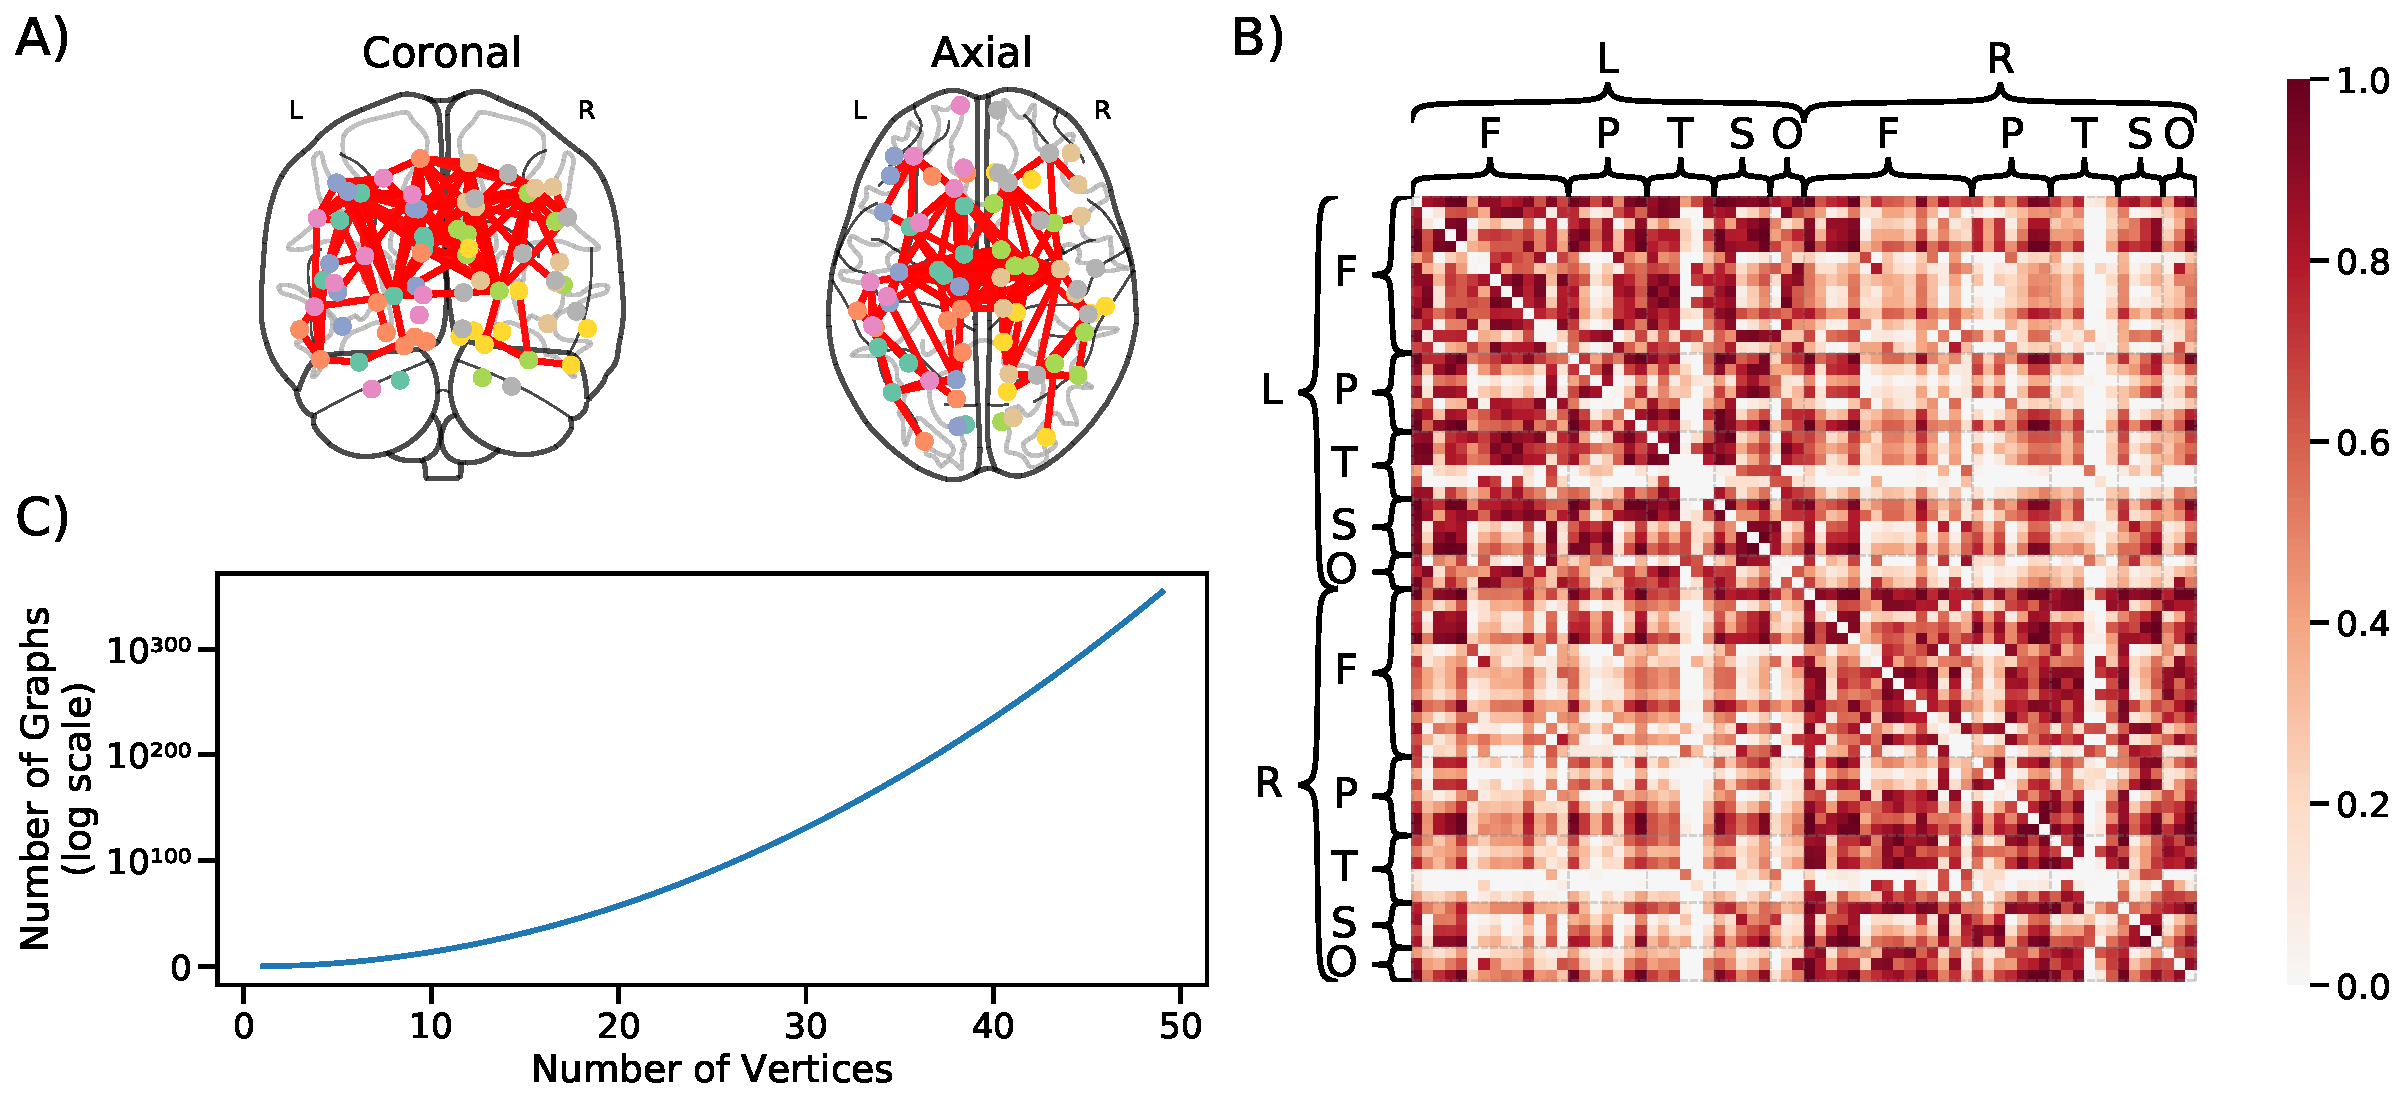
\includegraphics[width=\textwidth]{figures/dnd/intro}
    \caption{
    \textbf{Different Representations of a Connectome.} 
    Human structural connectome estimated from averaging 1059 human connectomes from the Human Connectome Project \citep{hcp1}.
    Vertices represent regions of the brain, and are assigned into right (R) and left (L) hemispheres and then further assigned into frontal (F), occipital (O), parietal (P), and temporal (T), and subcortical structures (S). 
    \textbf{a.} Connectivity shown in the coronal and axial views. Dots corresponds to the center-of-mass of the a region, lines correspond to connections, and line thickness corresponds to magnitude of the connection. Only the largest 5\% of edges are shown for visualization purposes. Note that infinitely many spatial arrangement of the vertices exist, and only one particular arrangement is being shown.
    \textbf{b.} Connectivity of the average structural connectome shown as an adjacency matrix, $\A$. The rows and columns are organized by hemisphere then further organized by sub-structures. However, given any permutation matrix $\Pbf$, the permuted adjacency matrix $\Pbf\A\Pbf^\top$ is still a valid matrix of original connectome. For a graph with $n$ vertices, there are $n^2$ permutations.
    \textbf{c.} The number of unique graphs grows exponentially as the number of vertices increases. The large number of graphs motivate statistical analysis to characterize and describe connectomes.
    } 
    \label{fig:intro_fig}
\end{figure}


\section{Representations}\label{sec:representations}
Due to the flexibility of networks, different representations of the connectomes can be studied, which we organize into four categories. In the following sections, we first formally define a network and then describe the four different frameworks of studying connectomics data. All frameworks provide complementary insights and understanding of the connectomes. 

\subsection{Graph/Network}
\label{sec:unwt_graph}
A graph, or network, $\mathcal{G}$, is defined as an ordered set of vertices and edges $(V, E)$ where $V$ is the vertex set, and $E$, the set of edges, is a subset of the Cartesian product of $V \times V$. That is, a graph has at most a single edge for each pair of unique vertices. A vertex set is represented as $V=\{1, 2, \ldots, n\}$ where $|V| = n$, and an edge exists between vertices $i$ and $j$ if $(i, j)\in E$. An unweighted graph is a graph in which we are only concerned with the presence (or absence) of an edge. Each graph has an associated adjacency matrix $\A \in \left\{0, 1\right\}^{n\times n}$ where $\A_{ij}$ represents the presence (or absence) of the edge between nodes $i$ and $j$. Note that $\A$ provides a unique representation of $\mathcal{G}$; that is, there exists a $1$-to-$1$ relationship between a graph and its adjacency matrix. 

The above definition can be further extended in two ways: 
\begin{enumerate}
    \item Weighted graphs - the edges can take on arbitrary values, typically a real number. For example, the edge weight in human structural connectomes are non-negative integers that represent the number of estimated neuronal fibers that traverse from one region of the brain to another. Thus, each weighted graph has an adjacency matrix $\A\in\RR^{n \times n}$ where $\A_{ij}$ represents the edge weight.
    \item Directed graphs - $E$ is now an \textit{ordered} set of edges. Each edge has an associated direction, and a directed edge exists between vertices $i$ and $j$ if $(i,j)\in E$. In undirected graphs, the associated adjacency matrix $\A$ is symmetric, but in directed graphs, $\A$ is not necessarily symmetric, that is, it is possible that $\A_{ij}\neq\A_{ji}$, for any $i, j\in V$.
\end{enumerate}

For the remainder of the paper, graphs are considered undirected and unweighted and with no self-loops, that is $\text{diag}(\A) = \Vec{0}$, unless specified otherwise.

\subsection{Bag of Features}\label{sec:bag-of-features}
Network statistics, or features, are abstract representations that capture either global or local structures of a network \citep{priebe_coppersmith_rukhin_2010,mhembere2013computing}. This method computes a set of network statistics for each network, and analyzes differences between, or among, populations. For example, when comparing populations of networks from healthy and individuals with depression, the difference in global clustering coefficient, which measures how likely vertices tend to cluster together, can be computed \citep{Bullmore2009-yj}. These network statistics have enjoyed applications in many connectomics studies that compare different populations of networks \citep{bullmore2011brain, ghoshdastidar2017two}. However, there are infinitely number of such statistics, and we lack general guidance in which statistics to compute. Furthermore, no set of network statistics can adequately characterize a network \citep{chen2018same,matejka2017same}. These considerable shortcomings further motivates the use of other representations of networks, and below examples demonstrate the shortcomings of studying bags of features.

\subsubsection{Non-identifiability of graph features}
Summary statistics, such as the mean, variance, and correlation, are often used to describe real valued datasets, which can be insightful in understanding the data. However, the Anscombe's quartet illustrates four drastically different distributions of eleven points that have the same summary statistics \citep{anscombe1973graphs}. This suggest that any small number of summary statistics can fail to meaningfully characterize the data. 

In network analysis, variety of network level statistics can be computed to summarize networks. Similar to the Anscombe's quartet, networks with different topologies can have the same network features as shown in Figure \ref{fig:exp5}. These four networks have the same number of vertices, edges, triangles, and global clustering coefficient, but have different properties such as connectedness and symmetry. Other works have also explored the distributions of network statistics \citep{chen2018same,matejka2017same}. 

\begin{figure}
    \centering
    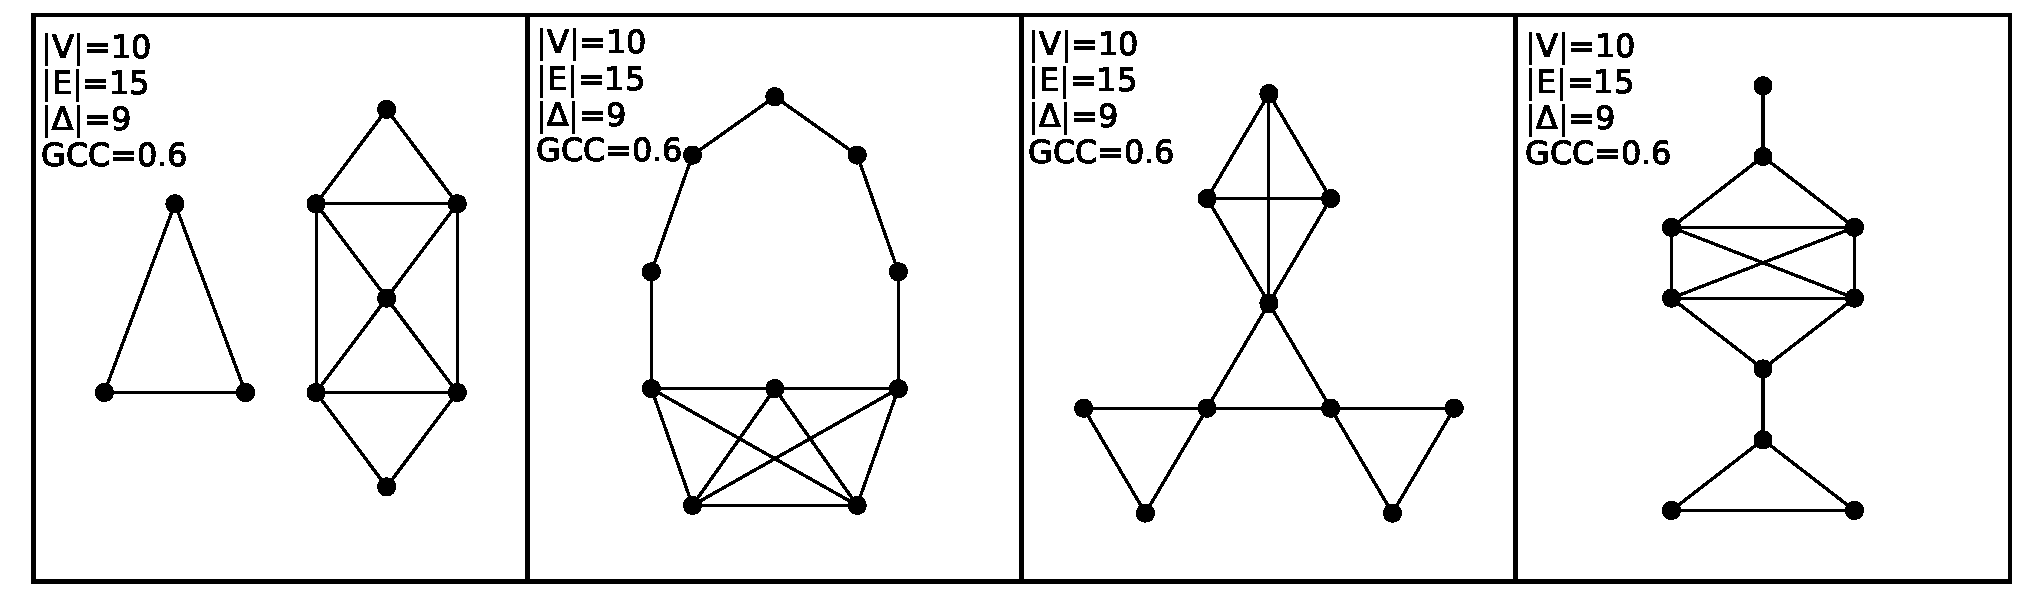
\includegraphics[width=.9\textwidth]{figures/dnd/exp5_10nodes_row}
    \caption{
    \textbf{Four Networks with Same Network Statistics.} Each network has 10 vertices ($\abs{V}$), 15 edges ($\abs{E}$), 9 triangles ($\abs{\Delta}$), and the global clustering coefficient (GCC) is 0.6. However these graphs have distinctive topologies. For example, the left-most network is disconnected, while others are connected. This suggest that given a small set of network statistics, one cannot identify from which network the features are computed.
    }
    \label{fig:exp5}
\end{figure}

\subsubsection{Network features are correlated and relatively uninformative}
We consider all non-isomorphic, undirected, binary networks with 10 vertices, which results in $\approx12$ million networks. Formally, $\mathcal{G}$ and $\mathcal{H}$ are isomorphic networks when there exists a vertex permutation function $f:V(\mathcal{G})\rightarrow V(\mathcal{H})$ such that if edge $(u,v)\in E(\mathcal{G})$, then $(f(u), f(v))\in E(\mathcal{H})$. Only non-isomorphic networks are considered since isomorphic networks have identical network features.

For each network, the following six graph network statistics are computed: 1) average path length (APL), 2) global clustering coefficient (GCC), 3) average clustering coefficient (ACC), 4) global efficiency (GE), 5) local efficiency (LE), and 6) modularity. These statistics are some of the most commonly computed statistics \citep{sporns2005human,Bullmore2009-yj}. The distribution of network statistics are plotted against modularity. 
The top row of Figure \ref{fig:exp6} shows that all of the network features are highly correlated with modularity.
We then constrain the networks in two different ways. First, we consider all networks with $20 \pm 2$ edges. Second, we choose a ``base'' network at random with 20 edges, and then identify all networks with no more than 3 edges different from the  base network. The distribution of each of the above network statistics on this subset of networks are computed for both constraints. The middle and bottom rows of Figure \ref{fig:exp6} show that constraining the networks in these ways hardly constrains the network features at all. Similar pattern is shown in the analysis of HCP data as shown in Supplemental Appendix \ref{sec:bag-of-features-hcp}. Changing only a few edges on a network can yield a network with almost any possible configuration according to these statistics, and therefore are inadequate to characterize these populations. Thus, when any given metric is correlated with a covariate of interest, so are many other metrics. Thus, claiming that a particular property of the brain ``explains'' a given phenotypic property of a person is spurious reasoning.

\begin{figure} 
    \centering
    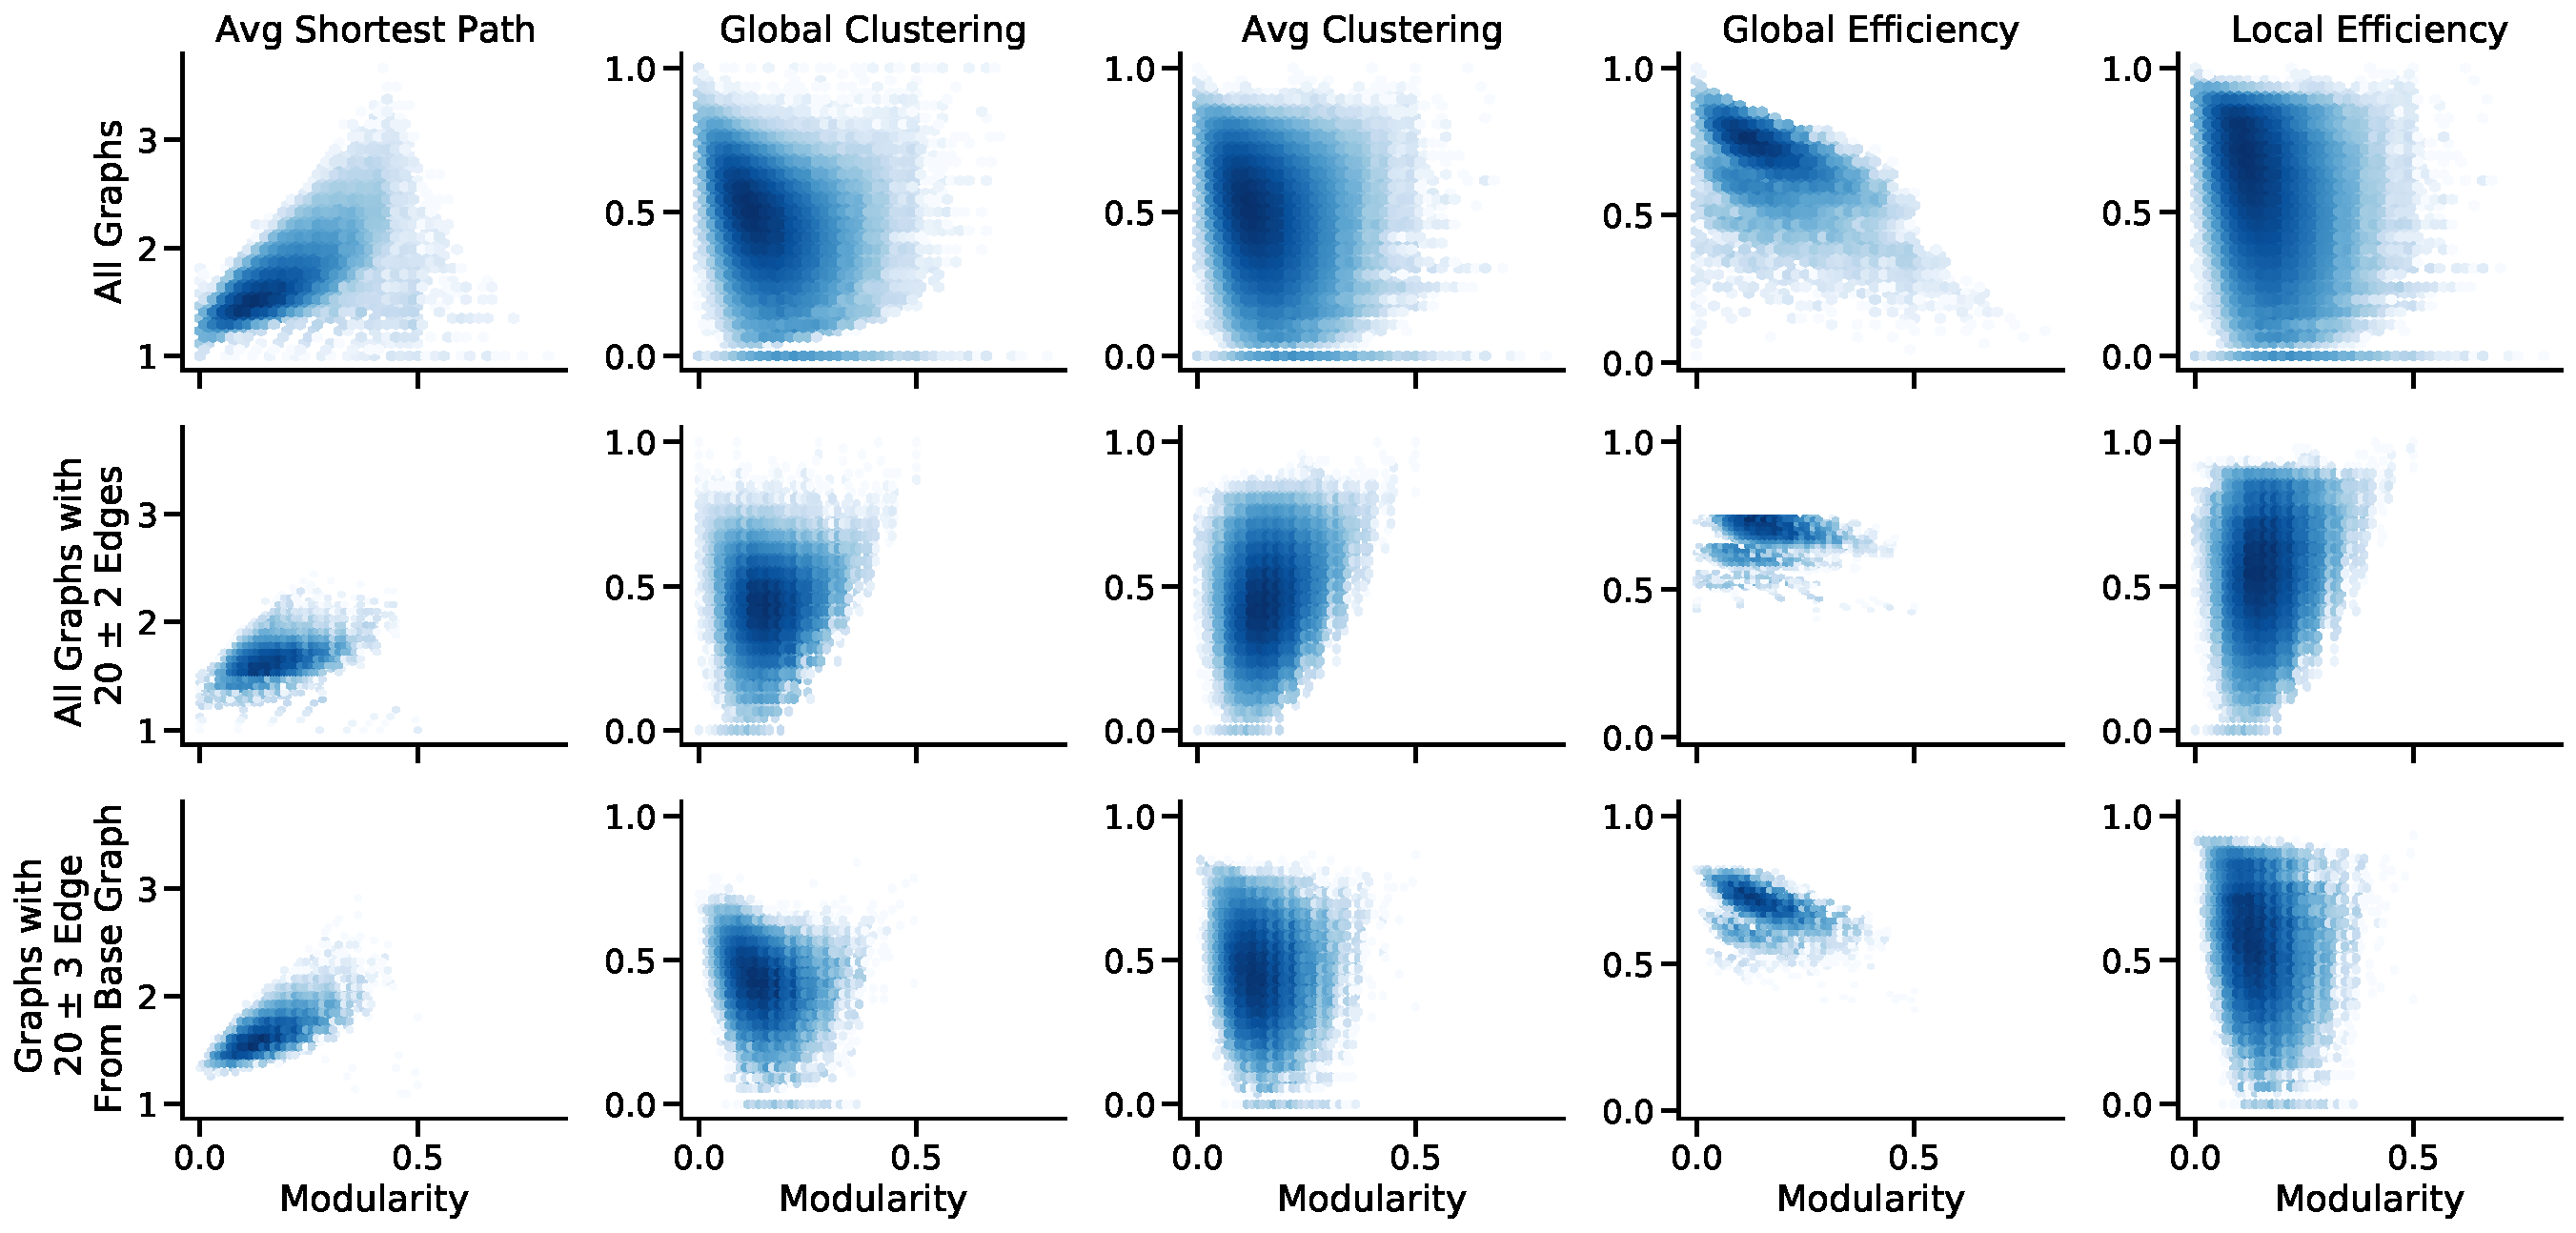
\includegraphics[width=\textwidth]{figures/dnd/density_num_edge_20_row}
    \caption{\textbf{Density plots of network statistics.} \textit{(Top Row)} The distributions of networks statistics for all possible 10-node networks are shown. \textit{(Middle Row)} Networks are constrained by only considering all networks with $20 \pm 2$ edges. \textit{(Bottom Row)} A base graph with $20$ edges is chosen at random, and only networks that have differences up to $3$ edges are considered. In both constrained set of networks, the distribution of these network statistics remains essentially unchanged. In other words, changing only a few edges on a network can yield a network with almost any possible configuration according to these statistics. }
    \label{fig:exp6}
\end{figure}

\subsection{Bag of Edges}\label{sec:bag_of_edges}
In this approach, the edges of connectomes are studied. Most commonly, each edge is studied independently, while ignoring any interactions between edges \citep{Craddock2013-qs,Varoquaux2013-hy,zhang2018mapping}. Univariate edge-wise testing can reveal easily interpretable relationships between specific edges and covariates through hypothesis testing. However, edge-wise testing requires performing multiple hypothesis tests, and multiple comparisons must be corrected to control the false positive rate \citep{Genovese2002-yq,Efron2008-zq}. While certain methods, such as Benjamini–Hochberg corrections, have strong theoretical guarantees, they require assumptions about the data, such as independence, that connectomics data do not satisfy \citep{Zalesky2010-ox,Benjamini1995-ij,Simes1986-gn}. On the other hand, Bonferroni corrections are considered too conservative, and, therefore, lack the sensitivity for connectomics \citep{Simes1986-gn}.

More intricate methods represent each connectome as a long vector containing all of its edges \citep{richiardi2011decoding, amico2017mapping}. Vector representations can allow for correlation of edges and direct application of common machine learning algorithms, but still discards the structural information in networks.

\subsection{Bag of Vertices}\label{sec:bag_of_nodes}
In this approach, the vertices of connectomes are analyzed while leveraging structural information, typically global structures, of the graphs. 
A common approach embeds the connectomes to learn a low-dimensional and Euclidean representation of the vertices \citep{grover2016node2vec, athreya2017statistical, arroyo2019inference}. Algorithms that operate on Euclidean data (e.g. Gaussian Mixture Model ($\gmm$) for clustering vertices, random forests for classifying vertices, multivariate hypothesis tests for testing for differences between vertices) can be employed for subsequent analysis \citep{priebe2017semiparametric, tang2018connectome}. 

\subsection{Bag of Communities}
Networks often contain structural information such as communities, which are subsets of vertices that behave similarly. For example, similar vertices can be defined by those that are more likely to be connected with each other than to other vertices.
The set of communities that comprise a network, called community structure, can describe both the local and global patterns of the network. At local-scale, we can examine the properties of vertices that are within the same community. At global-scale, we can measure associations between connectivity patterns of communities across groups or other covariates \citep{faskowitz2018weighted, kim2019graph, arroyo2020simultaneous}. Furthermore, the community structure in spatial resolution connectomes from human MRI can be used to delineate regions of the brain, called parcellations \citep{thirion2014fmri}.

Community detection in networks have been studied extensively \citep{newman2013spectral, fortunato2016community}. Typically, the community structure is identified by modularity optimization methods \citep{clauset2004finding, blondel2008fast}. In this paper, we present spectral methods that rely on statistical models for community detection, which have strong statistical guarantees for recovering true communities \citep{sussman2012consistent, lyzinski2016community, athreya2017statistical, arroyo2019inference}.
It is important to note that analysis of communities depends on the performance of the community detection algorithms.

\subsection{Bag of Networks}
In this approach, one or more groups of networks are studied in various settings, such as one- and two-sample hypothesis testing, and classification, using some representation of networks. For example, bag of vertices representation can be used to test whether two networks are different \citep{tang2017nonparametric, tang2017semiparametric}. For studying more than two networks, geometry in the space of the networks is defined and are represented in that geometry, which are then used for finding differences across groups \citep{ginestet2017hypothesis, xia2019matrix, arroyo2019inference}.

Another group of methods finds subsets of vertices, or a subgraph, that contain the most information about certain covariates \citep{vogelstein2012graph, wang2018signal,  relion2019network, wang2019symmetric, guha2020bayesian}. Estimating signal subgraphs is useful since networks can be extremely large (i.e. millions of vertices), which present computational challenges, and can potentially improve the performance of subsequent inference tasks, such as classification. 
Different approaches for finding the subgraph have been proposed, but all approaches leverage the network topologies inherent in connectomics data. 

\begin{table}
\caption{Notations and symbols used in this paper}\label{tab1}
\begin{center}
\begin{tabular}{|@{}l|c@{}|@{}l|c@{}|}
\hline
Symbols & Description & Symbols & Description\\
\hline
$[n]$ & $\{1, 2, \ldots, n\}$ & $\Pbf$ & Edge connectivity probability matrix\\
$\mathcal{G}$ & Graph & $\B$ & Block connectivity probability matrix\\
$n$ & Number of nodes & $\vec{\tau}$ & Vertex community assignment vector\\
$\A$ & Adjacency matrix & $\M$ & Edge community assignment matrix\\
$\A_i$ & $i$-th row of $\A$ & $\X$ & Latent position matrix\\
$\A_{ij}$ & $(i,j)$ entry of $\A$ & $\hat{\X}$ & Estimated latent position matrix\\
$\A^{(l)}$ & $l$-th element in sequence of $\A$ & &\\
\hline
\end{tabular}
\end{center}
\end{table}

\section{Statistical Models}\label{sec:models}
Connectomes can be modelled using statistical models designed for network data \citep{goldenberg2010survey, kolaczyk2014statistical}. Statistical models consider the entire network as a random variable, including the inherent structure, dependencies within networks, and the noise in observed data. 
Thus, statistical models can formalize detecting similarities or differences for each of the representations in Section \ref{sec:representations}.
This section provides an overview of many statistical models for network data, including those designed for representing single and multiple networks. 

Section \ref{sec:single_graph_models} provides an overview of single graph models that have been extensively studied as well as recently introduced models in the order of least to greatest complexity. Figure \ref{fig:models}a shows the relationship between all the single graph models presented in this paper. Section \ref{sec:multi_graph_models} provides an overview of some models for multiple networks. While other statistical models for multiple network data exist \citep{zhang2018network, wang2019joint, nielsen2018multiple, Durante2017-fz}, we focus on  some recent models that are used in spectral inference for connectomics data. In Appendix \ref{sec:model_extensions}, we describe some extensions to these models. 

\begin{figure}
    \centering
    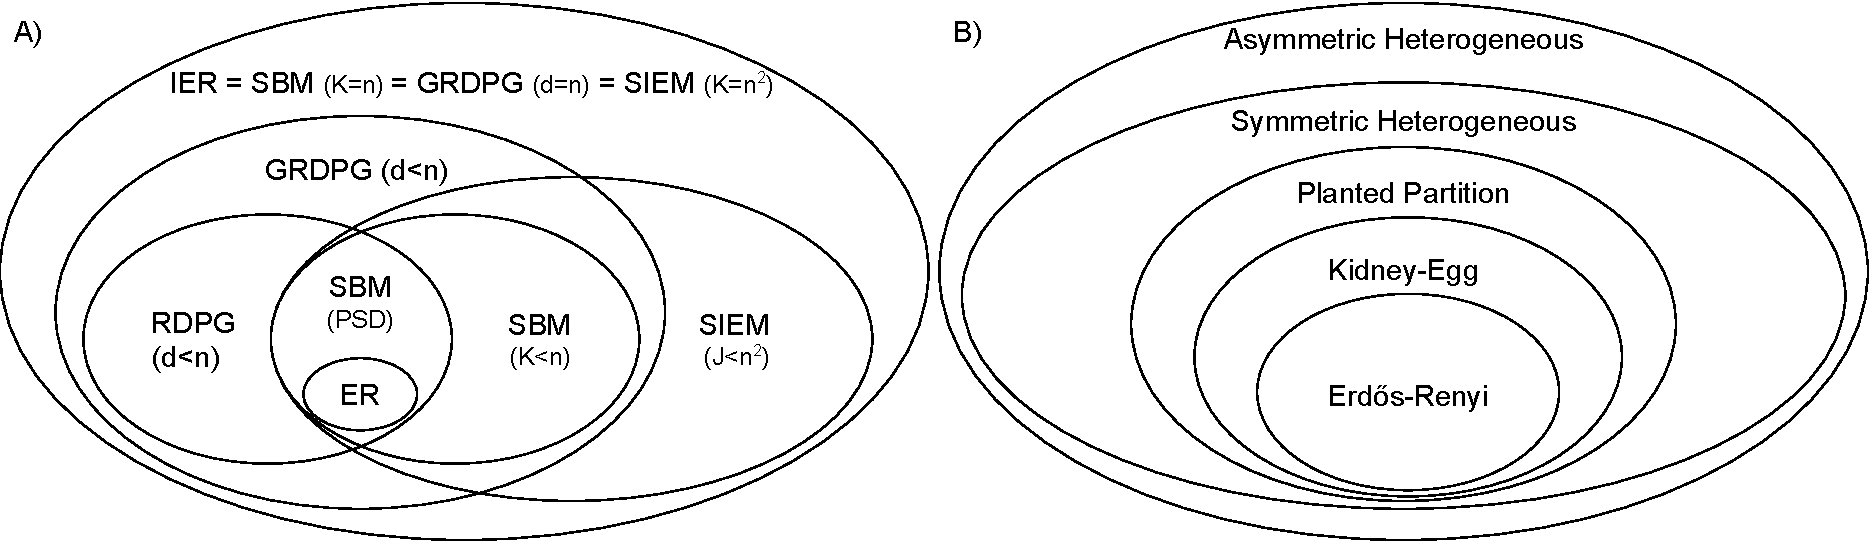
\includegraphics[width=\textwidth]{figures/dnd/models_combined}
    \caption{\textbf{Hierarchical Relationships of Statistical Models} 
    \textbf{(a)} Relationships among all the single-graph statistical models. Erd\H os-R\'enyi ($\er$) model is a stochastic block model ($\sbm$) with one community. $\sbm$ with a positive semidefinite block probability matrix $\B$ is also a random dot product graph ($\rdpg$). Any $\sbm$, $\rdpg$, and some structured independent edge model ($\siem$) can be represented as $d$-dimensional generalized random dot product graph ($\grdpg$) with $d$ less than number of vertices $n$. Inhomogenous Erd\H os-R\'enyi ($\ier$) model is equivalent to a $n$-block $\sbm$, $n$-dimensional $\grdpg$, and $n^2$-group $\siem$.
    \textbf{(b)} Relationships among the two-block $\sbm$ models. The most complex model is the asymmetric heterogeneous $\sbm$, and the simplest model is the $\er$, which is a degenerate case of 2-block $\sbm$.}
    \label{fig:models}
\end{figure}

\subsection{Single Graph Models}\label{sec:single_graph_models}
\subsubsection{Erd\H os-R\'enyi Random Graphs (ER)}\label{sec:uer}
The simplest random graph model is the $\mathsf{Erd\ddot{o}s-R\acute{e}nyi~(ER)}$ model \citep{Erdos1959-zf}. For a given set of $n$ vertices, each distinct pair of vertices are connected independently with probability $p \in [0, 1]$. Specifically, $\A \sim\er_n(p)$ if $\A$ has entries $\A_{ij}\sim\bern(p)$ for $i, j \in [n]$. While the $\er$ model is not representative of real data, it has been studied extensively since many of its properties can be solved exactly  \citep{newman2003random,Rukhin2010}.  

\subsubsection{Stochastic Block Model (SBM)}\label{sec:usbm}
First introduced in \cite{holland1983stochastic}, $\sbm$ is a model that can produce graphs with vertices grouped into $K$ communities \citep{Rohe2011-ha,sussman2012consistent,Wasserman1987-tw}. There are two simple variations of the $\sbm$ in which the vertex assignment vector $\vec \tau \in \left\{1, \hdots, K\right\}^n$ is known \textit{a priori}, and where $\vec \tau$ is not known. 
In both cases, a symmetric $K \times K$ block connectivity probability matrix $\B$ with entries in $[0,1]^{K \times K}$ governs the probability of an edge between vertices given their block memberships. 

If $\vec \tau \in \left\{1, \hdots, K\right\}^n$ is known \textit{a priori}, the \textit{a priori} $\sbm$ is parametrized only by the block connectivity matrix $\B$, and the model is $\A \sim \sbm_n(\vec \tau,\B)$ if $\A$ has entries $\A_{ij} \sim \bern(\B_{kl})$ where $\tau_i = k, \tau_j = l$, for $i, j \in [n]$, and $k, l \in [K]$. In the case where $\vec \tau$ is not known, the \textit{a posteriori} $\sbm$ is additionally parameterized by a block membership probability vector $\vec{\pi} = [\pi_1,\dots,\pi_K]^\top$ on the probability simplex.
The model is $\A \sim \sbm_n(\vec \pi,\B)$ if $\A$ has entries $\A_{ij} \big | k=\tau_i, l=\tau_j \sim \bern(\B_{kl})$, where $\tau_i {\sim} \multinomial(\vec \pi)$ for $i = 1, \hdots, n$. 

Throughout the context of this paper, we will focus particularly on a few variations of the two-block $\sbm$ ($K=2$) with block connectivity matrix $\B = \begin{bmatrix}a & b \\ c & d \end{bmatrix}$, abbreviated as $\B = [a, b; c, d]$. The common variants include:
\begin{enumerate}
    \item $\mathsf{Kidney-Egg}$: $b = c = d$. In this model, one of the blocks has edges with a different probability than the others, but the remaining blocks are homogeneous, where $a \neq b$. Furthermore, when $b > a$, the model is referred to as core-periphery $\sbm$.
    \item $\mathsf{Planted~Partition}$: $a = d$ and $b = c$. In this model, the within-block edges share a common probability $a$, and the between-block edges share a common probability $b$, where $a \neq b$.
    \item $\mathsf{Symmetric~ Heterogeneous}$: $b = c$. In this model, the between-block edges share a common probability $b$, but the within-block edges have a disparate probabilities, where $a \neq b \neq d$. 
    \item $\mathsf{Asymmetric~ Heterogeneous}$: $a \neq b \neq c \neq d$. In this directed model, every block has a unique probability.
    \item $\mathsf{Erd\ddot{o}s-R\acute{e}nyi}$: $a=b=c=d$. In this degenerate model, all blocks have a common probability, and the partitioning is irrelevant. 
    \item $\mathsf{Homophilic/Assortative/Affinity}$: $a, d > b, c$. In this model, the within-block probabilities are greater than cross-block probabilities.
    \item $\mathsf{Disassortative}$: $ b, c > a, d$. In this model, the cross-block probabilities are greater than the within-block probabilities.
\end{enumerate}
Figure \ref{fig:models}b summarizes the relationships of $\sbm$ models.

\subsubsection{Structured Independent Edge Model (SIEM)}\label{sec:usiem}
$\siem$ is a generalization of $\sbm$ that produces graphs in which edges are grouped into one of $K$ clusters. Analogous to the vertex assignment vector of the \textit{a priori} $\sbm$, the $\siem$ features an edge community assignment matrix $\M \in \left\{1, \hdots, K\right\}^{n \times n}$ which is known \textit{a priori}. Given the community assignment matrix $\M$, the $\siem$ is $\A \sim \siem_n(\M, \vec p)$ if $\A_{ij} {\sim}\bern(p_k)$ where $\M_{ij} = k$, for $i, j \in [n]$ and $k \in [K]$. $\vec p = [p_1, \hdots, p_K]^\top \in [0, 1]^K$ is the edge probability vector which governs the probability of an edge between vertices. 

The \textit{a priori} $\sbm$ is a special case of $\siem$ in which edges are assigned to blocks $\M$ which respect the vertex assignment vector $\vec \tau$. For the purposes of this paper, we will consider a case that frequently comes up in neuroimaging, the $\mathsf{Homotopic~ SIEM}$, in which each vertex has a matched ``pair'' amongst other vertices. The edges corresponding to a pair $\M_{ij} = 2$ where $(v_i, v_j)$ are a pair of vertices sharing a property, and the edges corresponding to a non-pair are $\M_{ij} = 1$. A matched pair of vertices, for instance, could be homotopic brain regions (two brain regions with similar function but in opposing hemispheres of the brain).

\subsubsection{Random Dot Product Graphs (RDPG)}\label{sec:rdpg}
$\rdpg$ belongs to the class of latent position random graphs \citep{hoff2002latent}. In a latent position graph, every vertex has associated to it a (typically unobserved) \textit{latent position} in some space $\mathcal{X}$, and the probability of connection between vertices $i$ and $j$ are given by a link function. In $\rdpg$, the space $\mathcal{X}$ is a constrained subspace of Euclidean space $\RR^d$ and the link function is the dot product \citep{Young2007-vu,scheinerman2010modeling,Sussman2014-zq}. Thus, in a $d-$dimensional $\rdpg$ with $n$ vertices, the matrix $\X\in \RR^{n\times d}$ whose rows are the latent positions, and the matrix of connection probabilities is given by $\Pbf=\X\X^\top$, which is positive semidefinite. The model is $\A\sim \rdpg_n(\X)$ if the adjacency matrix $\A$ has entries $\A_{ij} \sim \bern(\X_i\X_j^\top)$.
Subsequent inference tasks include community detection \cite{sussman2012consistent}, vertex classification \cite{tang2013}, or two-sample hypothesis testing for graphs with matched and non-matched vertices for a pair of graphs  \citep{priebe2019two,tang2017nonparametric,tang2017semiparametric}.

The $\rdpg$ is a flexible model, and other models of interest can be seen as special cases of the $\rdpg$. A $\sbm$ whose block connectivity matrix $\B$ is positive semi-definite is a $\rdpg$ with $K$ distinct latent positions. Thus, a $\sbm$ with $K$ blocks can be represented with a latent position matrix $\X\in\RR^{n\times d}$, with $d\leq K$, where there are only $K$ different rows of $\X$, and letting $\X_{\mathcal{U}}\in\RR^{K\times d}$ be the matrix with the subset of the rows $\mathcal{U}$ where each row is the latent position for a block, then the block connectivity matrix is $\B= \X_\mathcal{U}\X_\mathcal{U}^\top \in\RR^{K\times K}$. More generally, the $\rdpg$ can represent other models with more complex structures, such as mixed memberships \citep{Airoldi2008-tp} or hierarchical communities \citep{Lyzinski2017-cq}.

\subsubsection{Generalized Random Dot Product Graphs (GRDPG)}\label{sec:grdpg}
Unlike $\rdpg$ model, $\grdpg$ does not assume that $\Pbf$ is a positive semidefinite probability matrix  \citep{rubin2017statistical}. In this model, the edge probability matrix is given by $\Pbf=\X \I_{pq}\X^\top$, and $\A\sim\grdpg_n(
\X, p, q)$ if $\A_{ij}\sim\bern(\X_i\I_{pq}\X_j^\top)$ where $\I_{pq}=\textrm{diag}(1, \ldots, 1, -1, \ldots, -1)$  with $p$ ones followed by $q$ minus ones on its diagonal, and where $p \geq 1$ and $q \geq 0$ are two integers satisfying $p + q = d$.

The $\grdpg$ generalizes all of the previous models. When $q=0$, $\grdpg$ reduces to a $\rdpg$ model. To represent any $\sbm$ as $\grdpg$, let $p\geq 1, q\geq 0$ be the number of positive and negative eigenvalues of the block connectivity matrix $\B\in\RR^{K\times K}$, respectively. The block matrix can be represented as $\B = \X_\mathcal{U}\I_{pq}\X_\mathcal{U}^\top$.


\subsubsection{Inhomogenous Erd\H os-R\'enyi Random Graphs (IER)}\label{sec:uierrg}
The $\mathsf{Inhomogenous~Erd\ddot{o}s-R\acute{e}nyi~(IER)}$ is a model where each pair of nodes has a unique probability of an edge existing between the two, and is therefore the most general independent edge model. For a given set of $n$ vertices, the $\ier$ is parametrized by a matrix $\Pbf \in [0, 1]^{n \times n}$, where $\Pbf_{ij}$ is the probability of an edge connecting vertices $v_i, v_j$ where $i, j \in [n]$. That is, $\A \sim \ier_n(\Pbf)$ if $\A$ has entries $\A_{ij}\sim \bern(\Pbf_{ij})$ for $i, j \in [n]$. $\ier$ cannot be estimated from a single graph, as there are $n\choose 2$ unknowns (the probabilities) with $n\choose 2$ total observations (the edges).

Note that all single graph models are special cases of $\ier$. Additionally, $\sbm$ with $K=n$, $\siem$ with $K=n^2$, and $\grdpg$ with $d=n$ are equivalent to an $\ier$ model.

\subsection{Multiple Graph Models}\label{sec:multi_graph_models}

A common idea in statistical models for multiple graphs is a shared latent space that contain structural information common to all graphs. The two models presented in this section constrain the shared latent space in different ways to describe the heterogeneity in graphs, which results in sensitivity to different kinds of heterogeneity. The advantages and disadvantages of each model are highlighted in Section \ref{sec:multi_app}.

In the following models, consider a sample of $m$ observed graphs $\mathcal{G}^{(1)}, \mathcal{G}^{(2)}, \ldots, \mathcal{G}^{(m)}$  and their associated adjacency matrices, $\A^{(1)}, \A^{(2)}, \ldots, \A^{(m)}\in\RR^{n\times n}$ with $n$ vertices that are identical and shared across all graphs. 

\subsubsection{Joint Random Dot Product Graphs (JRDPG)}
In this model, we consider a collection of $m$ $\rdpg$s all with the same generating latent positions. Similar to a $\rdpg$, given an appropriately constrained Euclidean subspace $\RR^d$, the model is parameterized by a latent positions matrix $\X\in\RR^{n\times d}$ where $d \ll n$. The model is $\left(\A^{(1)}, \A^{(2)}, \ldots, \A^{(m)}\right)\sim \jrdpg(\X)$ where $\A_{ij}^{(l)}\sim \bern(\X_i\X_j^\top)$ for all $i, j \in [n]$ and $l\in [m]$. Each graph has marginal distribution $\A^{(l)}\sim\rdpg(\X)$ for all $l \in [m]$, meaning that the matrices $\A^{(1)}, \ldots,\A^{(m)}$ are conditionally independent given $\X$ \citep{athreya2017statistical,levin2017central}. While the model assumes that the latent positions for the graphs are the same, we note that this assumption is likely violated in heterogeneous networks, but still remains a very useful model as shown in Section \ref{sec:multi_app}.

\subsubsection{Common Subspace Independent-Edge Model (COSIE)} \label{sec:cosie}
In this model, the heterogeneous networks are described via a shared latent structure on the vertices, but also permits sufficient heterogeneity via individual matrices for each graph  \citep{arroyo2019inference}.
The model is parameterized by a  matrix $\V\in\RR^{n\times d}$ with orthonormal columns, 
where $n$ is the number of vertices and $d\ll n$, and  symmetric individual score matrices $\R^{(i)}\in\RR^{d\times d}$. The matrix $\V$ characterizes a low-rank common subspace, and is related to the latent positions for the vertices, and the score matrices incorporate individual differences to model the heterogeneity of the graphs. The model is denoted by $\left(\A^{(1)}, \ldots, \A^{(m)}\right)\sim \cosie(\V; \R^{(1)}, \ldots, \R^{(m)})$ where $\A_{ij}^{(l)} \sim \bern(\mathbf{P}^{(l)}_{ij})$ for all $i, j\in [n], i < j$, and $\mathbf{P}^{(l)}=\V\R^{(l)}\V^\top$. This factorization of the expected adjacency matrices is related to other decompositions for multiple matrices into population singular vectors or eigenvectors and individual parameters \citep{afshin2012enhancing,crainiceanu2011population,lock2013joint,wang2019common}.


\subsubsection{Correlated Models} \label{sec:correlated-graphs}


Finally, we are interested in graph models for a pair of graphs, $\mathcal{G}_1$ and $\mathcal{G}_2$, where the two graphs are said to be correlated; that is, the edges adjoining incident vertices have a non-zero correlation. Correlated graph models have numerous applications, such as when a graph is estimated repeatedly for the same source at different points in time.

\paragraph{Correlated $(\Pbf,\Q)$}
The $\mathbf{R}$-correlated $(\Pbf, \Q)$ model \citep{lyzinski2017matchability} with parameters $\mathbf{R}, \Pbf, \Q\in[0,1]^{n\times n}$, denoted as $\mathrm{CorrER}(\Pbf, \Q, \mathbf{R})$, produces two graphs $\mathcal{G}_1$ and $\mathcal{G}_2$ with adjacency matrices $\A^{(1)}, \A^{(2)}$ such that each graph is marginally an inhomogeneous Erd\H{o}s-R\'enyi with $\A^{(1)} \sim \ier(\Pbf)$, $\A^{(2)}\sim \ier(\Q)$, but the  pairs of corresponding edges have Pearson correlation  encoded in the matrix $\mathbf{R}$ such that 
$$\mathbf{R}_{ij} = \text{Corr}(\A^{(1)}, \A^{(2)})= \frac{\mathbb{P}(\A^{(1)}_{ij}=\A^{(2)}_{ij}=1)-\Pbf_{ij}\Q_{ij}}{\sqrt{\Pbf_{ij}(1-\Pbf_{ij}) \Q_{ij}(1-\Q_{ij})}}.$$
When $\Pbf$ and $\Q$ are different, there are restrictions in the values that the correlation matrix $\mathbf{R}$ can take. In particular, if $\Pbf_{ij}\neq\Q_{ij}$  and $\Pbf>\Q$, then $\mathbf{R}_{ij}\leq \sqrt{\frac{\Q_{ij}(1-\Q_{ij})}{\Pbf_{ij}(1-\Pbf_{ij})}}$ \citep{lyzinski2017matchability}.


We are interested particularly in two special cases of the $\mathrm{CorrER}(\Pbf, \pmb Q, \pmb R)$:
\begin{enumerate}
    \item The $\rho$-correlated $\rdpg$ model arises when $\Pbf = \Q=\X\X^\top$ for some latent position matrix $\X \in \RR^{n \times d}$  as in Section \ref{sec:rdpg}, and $\pmb R = \rho \pmb 1_{n \times n}$ (that is, the matrix of edge correlations $\pmb R$ has only a single unique entry $\rho\geq 0$). We say that $\A_1, \A_2 \sim \rho\rdpg(\X)$.
    \item The $\rho$-correlated $\er$ model arises in the case where $\Pbf = \Q = p\pmb 1_{n \times n}$ (i.e.,  the probability matrix has a single unique entry $p>0$), and $\pmb R = \rho\pmb 1_{n \times n}$ (as above, the matrix of correlations has a single unique entry). We say that $\A_1, \A_2 \sim \rho\er(p)$.
\end{enumerate} % review
\chapter[Two-Sample Graph Testing]{Valid Two-Sample Graph Testing via Optimal Transport Procrustes and Multiscale Graph Correlation with Applications in Connectomics} \label{chap:nonpar}

This chapter introduces
This chapter documents our first investigation into the alpha blocker treatment hypothesis in humans facing a severe respiratory illness. Importantly, this study leveraged large insurance claims databases and common health conditions during a period where the COVID-19 data environment was too immature to produce a sufficiently large and well-understood sample for this analysis. This chapter was originally published in Stat in October 2021 (DOI:  \url{https://doi.org/10.1002/sta4.429}) and is distributed under the terms of a Creative Commons Attribution License that permits unrestricted use and redistribution provided that the original author and source are credited.

\begin{singlespace}         % you can also use onehalfspace to relax the spacing
    \fullcite{chung2022valid} \mybibexclude{chung2022valid}
\end{singlespace} 

\pagebreak
\section*{Abstract}
Testing whether two graphs come from the same distribution is of interest in many real world scenarios, including brain network analysis.
Under the random dot product graph model, the nonparametric hypothesis testing framework consists of embedding the graphs using the adjacency spectral embedding (ASE), followed by  aligning the embeddings using the median flip heuristic, and finally applying the nonparametric maximum mean discrepancy (MMD) test to obtain a p-value.
Using synthetic data generated from \textit{Drosophila} brain networks, we show that the median flip heuristic results in an invalid test, and demonstrate that optimal transport Procrustes (OTP) for alignment resolves the invalidity.
We further demonstrate that substituting the MMD test with multiscale graph correlation (MGC) test leads to a more powerful test both in synthetic and in simulated data.
Lastly, we apply this powerful test to the right and left hemispheres of the larval \textit{Drosophila} mushroom body brain networks, and conclude that there is not sufficient evidence to reject the null hypothesis that the two hemispheres are equally distributed.

\pagebreak

\section{Introduction}\label{sec:introduction}
A network, or graph, is a data type which naturally encodes information about relationships between variables.
Statistical network analysis is becoming an increasingly important area \cite{goldenberg2010survey}, as it has applications in fields such as brain \cite{bullmore2009complex} and social sciences \cite{wasserman1994social}. Often, we encounter more than one graph observation, and it is  scientifically interesting to determine whether the two graphs come from the same distribution: the \textit{two-sample graph hypothesis testing} problem. 
When the two samples are real-valued scalars, procedures such as the $t$-test and Wilcoxon rank-sum test are available, but these methods do not generalize to more complex data types such as networks.

Recently, methods have been proposed for determining whether two graphs are statistically equivalent under different settings \cite{semipar, omni, tang2014nonparametric, graph-comparison-same-1, graph-comparison-same-3, graph-comparison-same-4, graph-comparison-other-1, graph-comparison-other-2, graph-comparison-other-5, graph-comparison-other-8, graph-comparison-other-9}.
Most of these methodologies are aimed for pairs of graphs with a known correspondence between their vertices, and thus the problem consist in finding significant differences on the corresponding edges or vertices. 
Here, we focus on the more general setting where this vertex correspondence is unknown or might not exist, for example when the graphs do not have the same number of vertices. 
In this setting, we are interested in identifying significant differences on some underlying structure of the vertices.
In particular, \cite{tang2014nonparametric} proposed a nonparametric approach that operates on pairs of graphs in which there is no known correspondence between their corresponding vertex sets using the distance between probability distributions on a vertex latent space. This method uses the maximum mean discrepancy (MMD) test to detect differences between  distributions of the estimated latent positions of the vertices.
In \cite{agterberg2020nonparametric}, the authors extend this procedure to resolve the inherent non-identifiabilities in the vertex latent space via an optimal transport solution that yields consistent nonparametric hypothesis test.
% study a similar test statistic when there is nonidentifiabilities between the estimated vertex latent space, 
% random graphs with both negative and repeated eigenvalues and sparsity, 
% and they show that properly aligning the respective latent space yields consistent nonparametric hypothesis testing. 

MMD has been shown to be equivalent to the Energy distance two-sample test, the Hilbert-Schmidt independence
criterion (HSic), and the distance correlation test for independence (DCorr) \cite{exact-equivalence-1, exact-equivalence-2}. 
HSic and DCorr, which are independence tests, are used as two-sample tests via first performing a \textit{k-sample transform}, which consists of concatenating the two samples, defining an auxiliary label vector, and subsequently testing for independence of the samples and label vector \cite{exact-equivalence-2}.
Multiscale graph correlation (MGC) is a recently proposed measure of dependence that
has shown an improved empirical power in many settings by intelligently selecting the appropriate
scale of the data \cite{mgc-0, mgc-1, mgc-2}. In this paper, we propose a new methodology for testing equivalence of distributions between networks using MGC as the test statistic. We demonstrate empirically in multiple simulation and synthetic data settings that
MGC outperforms other methods, and demonstrate its use on the problem of comparing the connectivity of the brain hemispheres of the \textit{Drosophila melanogaster}.

\section{Background}\label{sec:background}
\subsection{Graphs and Embeddings}
A graph $G = (\mathbb{V}, \mathbb{E})$ with $n$ vertices is composed of a vertex set $\mathbb{V} = \{v_1, \dots, v_n\}$ and an edge set $\mathbb{E} \subseteq \mathbb{V} \times \mathbb{V}$, where the edge $(v_i,v_j)\in\mathbb{E}$ connects vertices $i$ and $j$. Graphs can be represented by an adjacency matrix $A\in\{0,1\}^{n\times n}$, with rows and columns corresponding to vertices and matrix entries corresponding to edge values, so $A_{ij}=1$ whenever $(v_i,v_j)\in\mathbb{E}$.

The \textit{random dot product graph} (RDPG) model \cite{athreya2018rdpg} treats the entries of an adjacency matrix $A$ as independent Bernoulli random variables, where the probability of an edge is given by the dot product of pairs of latent positions $x_1,\ldots, x_n\in\mathbb{R}^d$ for each vertex, so $\mathbb{P}(A_{ij}=1) = x_i^\top x_j$. These latent positions are independent random variables sampled according to some distribution $F$. Writing $X = \left[x_1 \cdots x_n\right]^\top$ as the matrix of latent positions, we denote $(X,A)\sim\text{RDPG}_n(F)$ as a RDPG with adjacency matrix $A$ and (usually unobserved) latent positions $X$ sampled from $F$. With this notation, we have that $\mathbb{E}(A|X) = XX^{\top}$. 

The RDPG model provides a flexible framework for studying the statistical equivalence of a pair of graphs. Suppose that $(X,A)\sim\text{RDPG}_n(F_X)$ and $(Y,B)\sim\text{RDPG}_m(F_Y)$. 
Then, the two graphs $A$ and $B$ are said to have the same distribution if there exists an orthogonal matrix $W\in\mathbb{R}^{d\times d}$, $W^\top W = I$ that makes $X$ and $W^\top Y$ have the same distribution. 
The matrix $W$ accounts for the nonidentifiability inherent with inner products \cite{tang2014nonparametric}. 
Formally, this hypotheses test can be stated as 
  \begin{align*}
    &H_0 : F_X = F_Y \circ {W}
    && \text{for some orthogonal operator } {W},\\
       &H_A : F_X \neq F_Y \circ {W}
    && \text{for all orthogonal operators } {W}.
  \end{align*}
Here, $F_Y\circ W$ denotes the distribution of the random variable $W^\top Y$. 
The graphs $A$ and $B$ do not need to have a correspondence between their vertices, or even
the same number of vertices, because we are comparing distributions of latent
positions instead of the latent positions themselves. 
This work focuses on cases where the number of vertices are equal, or approximately equal, that is $n \approx m$. 

Latent positions are typically unobserved in practice and can be estimated via the \textit{adjacency spectral embedding} (ASE) \cite{ase-consistency-1}.
Suppose that $A= USV^\top + U_\perp S_\perp V^\top_\perp$ is the singular value decomposition of $A$, where $U,V\in\mathbb{R}^{n\times d}$, $U_\perp,V_\perp\in\mathbb{R}^{n\times(n-d)}$ are jointly orthogonal matrices
corresponding to the singular vectors of $A$, and $S\in\mathbb{R}^{d\times d}$,
$S_\perp\in\mathbb{R}^{(n-d)\times (n-d)}$ are diagonal matrices such that $S$
contains the $d$ largest singular values of $A$. 
Then, the ASE of $A$ is defined as $\hat{X}=US^{1/2}$. This simple and computationally efficient approach results in consistent estimates $\hat{X}$ and $\hat{Y}$ of the true latent positions $X$ and $Y$ \cite{ase-consistency-1,ase-consistency-2, ase-consistency-3}.
The ASE depends on a parameter $d$ that corresponds to the rank of the expected adjacency matrix conditional on the latent positions; in practice, we estimate this dimension, $\hat d$ via the scree plot of the eigenvalues of the adjacency matrix which can be done automatically via a likelihood profile approach \cite{zhu2006automatic}.

If the two networks have large difference in the number of vertices, the subsequent testing procedure might be invalid due to the finite-sample variances of the estimated latent positions, $\hat{X}$ and $\hat Y$, that depend on the number of vertices \cite{Athreya2015}. Thus, the distributions of the estimated latent positions may not be the same even if the true distributions are the same. The difference in variances can be corrected by adding scaled Gaussian noise to the estimated latent positions of larger network, which increases the variance of the larger network to be approximately the same as that of the smaller network \cite{correcting-nonpar}. This correction results in a valid test for the equivalence of the distributions of latent positions. 


\subsection{Orthogonal Nonidentifiabilities}
There are two sources of an orthogonal nonidentifiability associated with using the
ASE in RDPG \cite{on-two-sources}. The first is associated with the RDPG model itself, and can take a form of any orthogonal transformation, since for any
orthogonal matrix $W$, it holds that $(XW)(XW)^\top = X W W^\top X^\top = X X^\top$. When
using ASE, this orthogonal matrix converges to a population value at the rate 
$O_p \left(n^{-1/2}\right)$, and, thus, rarely has any inferential consequences \cite{tang2014nonparametric, on-two-sources}.

The second source, called subspace nonidentifiability, is associated with taking a singular value decomposition as a part of the ASE. 
Consider the singular value decomposition of the matrix $XX^\top$.
Since it is positive semidefinite, its eigendecomposition and singular value decomposition coincide.
If $XX^\top$ has no repeated singular (eigen) values, then each singular (eigen) vector is determined only up to a sign ambiguity.
However, if $XX^\top$ has repeated eigenvalues, then the singular (eigen) vectors corresponding to each repeated singular value are only unique up to an orthogonal transformation in the dimension of the corresponding subspace.
Since one only observes two different adjacency matrices, then the leading singular vectors may not be aligned \textit{a priori}.
If one assumes that $XX^\top$ has distinct eigenvalues, this sign ambiguity is often adjusted for by flipping the signs of each dimensions such that the medians have the same sign; that is for each embedding dimension, $\text{sign}(\text{median}(X_i)) = \text{sign}(\text{median}(Y_i))$ for all $i\in d$ \cite{tang2014nonparametric, correcting-nonpar}. 
This heuristic can perform poorly when the medians of the samples are too close to zero.
In addition, this approach falls short in the case of repeated eigenvalues of the matrix $XX^{\top}$ since the subspace associated with such values are only unique up to a more general rotation, and hence the leading singular vectors of each adjacency matrix may not be close, even if $n$ is large, since the leading singular values of the adjacency matrices will be perturbed versions of the singular values of $XX^\top$. For more details and discussion on this form of nonidentifiability, see \cite{on-two-sources}. 

If the two graphs had paired vertices, then the orthogonal misalignment between the two samples could be resolved by using a solution to
a well-known orthogonal Procrustes problem \cite{schonemann1966generalized}.
In unpaired graphs, there is no \textit{a priori} assignment between vertices, so we can employ an Optimal Transport Procrustes (OTP) algorithm \cite{agterberg2020nonparametric}, which simultaneously solves the alignment and the assignment problems. Formally, this algorithm minimizes the objective function
\begin{align}
    \min_{W,  \Pi} \langle \Pi, C_W \rangle
    \label{eq:2.1}
\end{align}
where the entries of the cost matrix $C_W$ are given by $\left(C_W\right)_{ij} =  ||\hat X_i - W\hat Y_j||^2$,  $\hat X \in \mathbb{R}^{n\times d}$ and $\hat Y \in \mathbb{R}^{m\times d}$ are estimated latent positions,  $\Pi = \frac{1}{nm} \mathbf{1} \mathbf{1}^\top$ is an assignment matrix that satisfies $\Pi \mathbf{1} = \frac{1}{n} \mathbf{1}$ and $\Pi^{\top} \mathbf{1} = \frac{1}{m} \mathbf{1}$, and $W$ is constrained to be orthogonal. Given an initial guess $W_0$, the algorithm iteratively updates $\Pi_{i+1} | W_{i}$
by via an optimal transport algorithm \cite{alvarez2019towards} and $W_{i+1} | \Pi_{i}$ using the solution to the Procrustes problem. In graph setting, the algorithm is initialized with all possible orthogonal diagonal matrices, i.e. the 
$2^d$ different diagonal matrices with $\pm{1}$ on the diagonal \cite{agterberg2020nonparametric}. In \cite{agterberg2020nonparametric}, the authors show that the orthogonal matrix that globally minimizes the objective function \eqref{eq:2.1} yields a consistent estimate of the orthogonal matrix approximately aligning the empirical distributions of the two ASEs, including when the corresponding graphs have (asymptotically) repeated singular (eigen) values.

\subsection{Distance Correlation}
Due to the equivalence between two-sample and independence testing \cite{exact-equivalence-2}, distance correlations (DCorr) can be used to test the equality of the distributions $F_X$ and $F_Y$. Define $Z=(X^\top, Y^\top)^\top\in\mathbb{R}^{N\times d}$ and $E=(0_n, 1_m)^\top\in\mathbb{R}^{N}$, where $N=n+m$. DCorr tests the independence of $Z$ and $E$ using some distance functions $\delta_Z:\mathbb{R}^{d}\times\mathbb{R}^{d}\rightarrow\mathbb{R}$ and $\delta_E:\mathbb{R}\times\mathbb{R}\rightarrow\mathbb{R}$. Here, $\delta_Z$ and $\delta_E$ denote the Euclidean norm in $\mathbb{R}^{d}$ and $\mathbb{R}$, respectively.

First, DCorr computes distance matrices $D^Z, D^E$ such that $D^Z_{i,j} = \delta_Z(Z_i, Z_j)$ and $D^E_{i,j} = \delta_E(E_i, E_j)$. The distance matrices are then doubly centered to $D^{Z'}, D^{E'}$, where $D^{Z'}_{i,j} = D^Z_{i,j} - \overline{D^Z}_{\cdot,j} - \overline{D^Z}_{i,\cdot} + \overline{D^Z}_{\cdot,\cdot}$, and similarly for $D^{E'}$. Here the column means, row means, and the grand mean are $\overline{D^Z}_{\cdot, j} = \frac{1}{N}\sum_{i=1}^N D^Z_{i,j}$, $\overline{D^Z}_{i, \cdot} = \frac{1}{N}\sum_{j=1}^N D^Z_{ij}$, and $\overline{D^Z}_{\cdot, \cdot} = \frac{1}{N^2}\sum_{i=1}^N\sum_{j=1}^N D^Z_{ij}$, respectively. The sample DCorr test statistic \cite{szekely2014dcorr} is defined as
\begin{align*}
    \operatorname{DCorr}(Z,E) = \frac{1}{N(N-3)\sigma_{D^{Z'}}\sigma_{D^{E'}}}\sum_{i,j} D^{Z'}_{i,j}D^{E'}_{i,j},
\end{align*}
where $\sigma_{D^{Z'}}$ and $\sigma_{D^{E'}}$ are the standard deviation of values in $D^{Z'}$ and $D^{E'}$, respectively. A null distribution of this test statistic
can be generated by permuting the indices of $E$ or approximated using an asymptotic result \cite{shen2019chi}.
% TODONE cite cencheng's fast approximate paper here.

The centered versions $D^{Z'}, D^{E'}$ have the property that all rows and columns sum to zero, but the test statistic is biased for finite samples. An unbiased version of DCorr modifies the centering method of the pairwise distance matrices \cite{szekely2014dcorr}. This method, called U-centering, generates a matrix $D^{Z''}$ that has the additional property that $E[D^{Z''}_{ij}] = 0, i, j = 1, \dots, N$. $D^{Z''}$ uses a slightly different form for the row means, column means, and grand mean, given by $\widetilde{D^{Z}}_{\cdot, j} = \frac{1}{N-2}\sum_{i=1}^N D^{Z}_{ij}$ (similarly for row means) and $\widetilde{D^{Z}}_{\cdot, \cdot} = \frac{1}{(N-2)(N-1)}\sum_{i,j} D^{Z}_{ij}$. The test statistic is defined analogously modulo these new definitions.

\subsection{Multiscale Graph Correlation}
An alternative method for approaching the hypothesis testing problem is MGC \cite{mgc-0, mgc-1, mgc-2}, which uses the distance-based methods in DCorr, but also considers the local scale of the data.
MGC is based on unbiased DCorr, resulting in it also being unbiased. MGC consists of the following steps.

\begin{enumerate}
	\item Compute the centered distance matrices $D^{Z''}$ and $D^{E''}$.
	\item For each $k,l$ in $1,\ldots, N$, compute the $k$ and $l$ nearest neighbors of each row of $D^{Z''}$ and $D^{E''}$, respectively, and denote the induced nearest neighbor graphs by $G^k\in\{0,1\}^{N\times N}$ and $H^l\in\{0,1\}^{N\times N}$.
	\item Estimate the local normalized correlations $c^{k,l}$ such that
	\begin{equation*}
	c^{kl} = \frac{\sum_{i,j}D^{Z''}_{ij}D^{E''}_{ij}G^k_{ij}H^{l}_{ij}}{\left(\sum_{i,j}(D^{Z''}_{ij})^2G^k_{ij}\right) \left(\sum_{ij}(D^{E''}_{ij})^2H^{l}_{ij}\right)}.
	\end{equation*}
	\item Using a smoothing parameter $\tau$, estimate the smoothed maximum of $c^{kl}$ over all possible values of $k$ and $l$, defined as
	\begin{align*}
	R &= \text{LCC}\{(k,l):c^{kl}>\max(\tau,c^{NN})\},\\
    c^\ast &= \max_{(k,l)\in R}c^{kl},
	\end{align*}
	where LCC denotes the largest connected component of the graph defined by a set of edges.
\end{enumerate} 

Similar to DCorr, the null distribution of the test statistic, $c^\ast$, is generated by permuting the indices of $E$.
When the relationship is nonlinear or non-monotonic, MGC tends to choose scales smaller than $n$, detecting relationships more often than DCorr, and thus, it can be considered a direct generalization to the above methods, with often large finite sample power gains, with a minor running time cost \cite{mgc-0}.

\section{Simulations}\label{sec:simulations}

The performance of DCorr and MGC is analyzed by simulating graphs with different distributions. The graphs are simulated according to the RDPG model, using different distributions (described below) to generate their univariate latent positions $X=(x_1,\ldots, x_n)^\top$ and $Y=(y_1,\ldots, y_n)^\top$, and the latent positions are estimated via ASE with embedding dimension $\hat d= 1$. 
% TODONE is d=1, or dhat, or both? please clarify.
The sign ambiguity is resolved via median flip since the graphs are embedded into one dimension. The estimates are then used to compute the corresponding test statistics, and calculate the $p$-value after estimating the null distribution via permutation test. The tests reject at a significance level $\alpha=0.05$, and the empirical power is based on 1000 Monte Carlo replicates. This process is repeated for increasing numbers of vertices in each graph. The graph generating mechanisms are described next.

\paragraph{Equal distribution of the latent positions}
First, we analyze the performance of the methods when the null hypothesis is true, so the latent positions $X$ and $Y$ have the same distribution: $x_i \overset{\text{iid}}{\sim} F_X$ and $y_i \overset{\text{iid}}{\sim} F_X$, $i=1,\ldots,n$,
with
$F_X = \operatorname{Unif}(.2,.7)$.
That is, these mutually independent sets of latent positions are uniformly distributed on the range $(.2, .7)$.
Figure \ref{fig:simulations_nonpar} (left) shows the empirical size of the tests for different numbers of vertices. The empirical power does not exceed $\alpha$, showing that both DCorr and MGC correctly control the type I error.
 
\paragraph{Linear difference in the distributions}
For this setting, we generate $x_i \overset{\text{iid}}{\sim} F_X$ and $y_i \overset{\text{iid}}{\sim} F_X + 0.1$ (Figure \ref{fig:simulations_nonpar}, middle).
As the number of vertices in each graph increases, the difference between the distributions becomes easier to detect, and both DCorr and MGC algorithms detect the differences, resulting in power increasing to unity at equal rate for both methods.

\paragraph{Nonlinear difference in the distributions}
Finally, set $x_i \overset{\text{iid}}{\sim} F_X$ and $y_i \overset{\text{iid}}{\sim} 0.5\operatorname{Beta}(.2, .2)+0.2$. Figure \ref{fig:simulations_nonpar} (right) shows  the power of both DCorr and MGC goes to 1, but MGC dominates DCorr at  all sample sizes sample sizes until both tests achieve power of one.

\begin{figure}[hbt!]
    \centering
    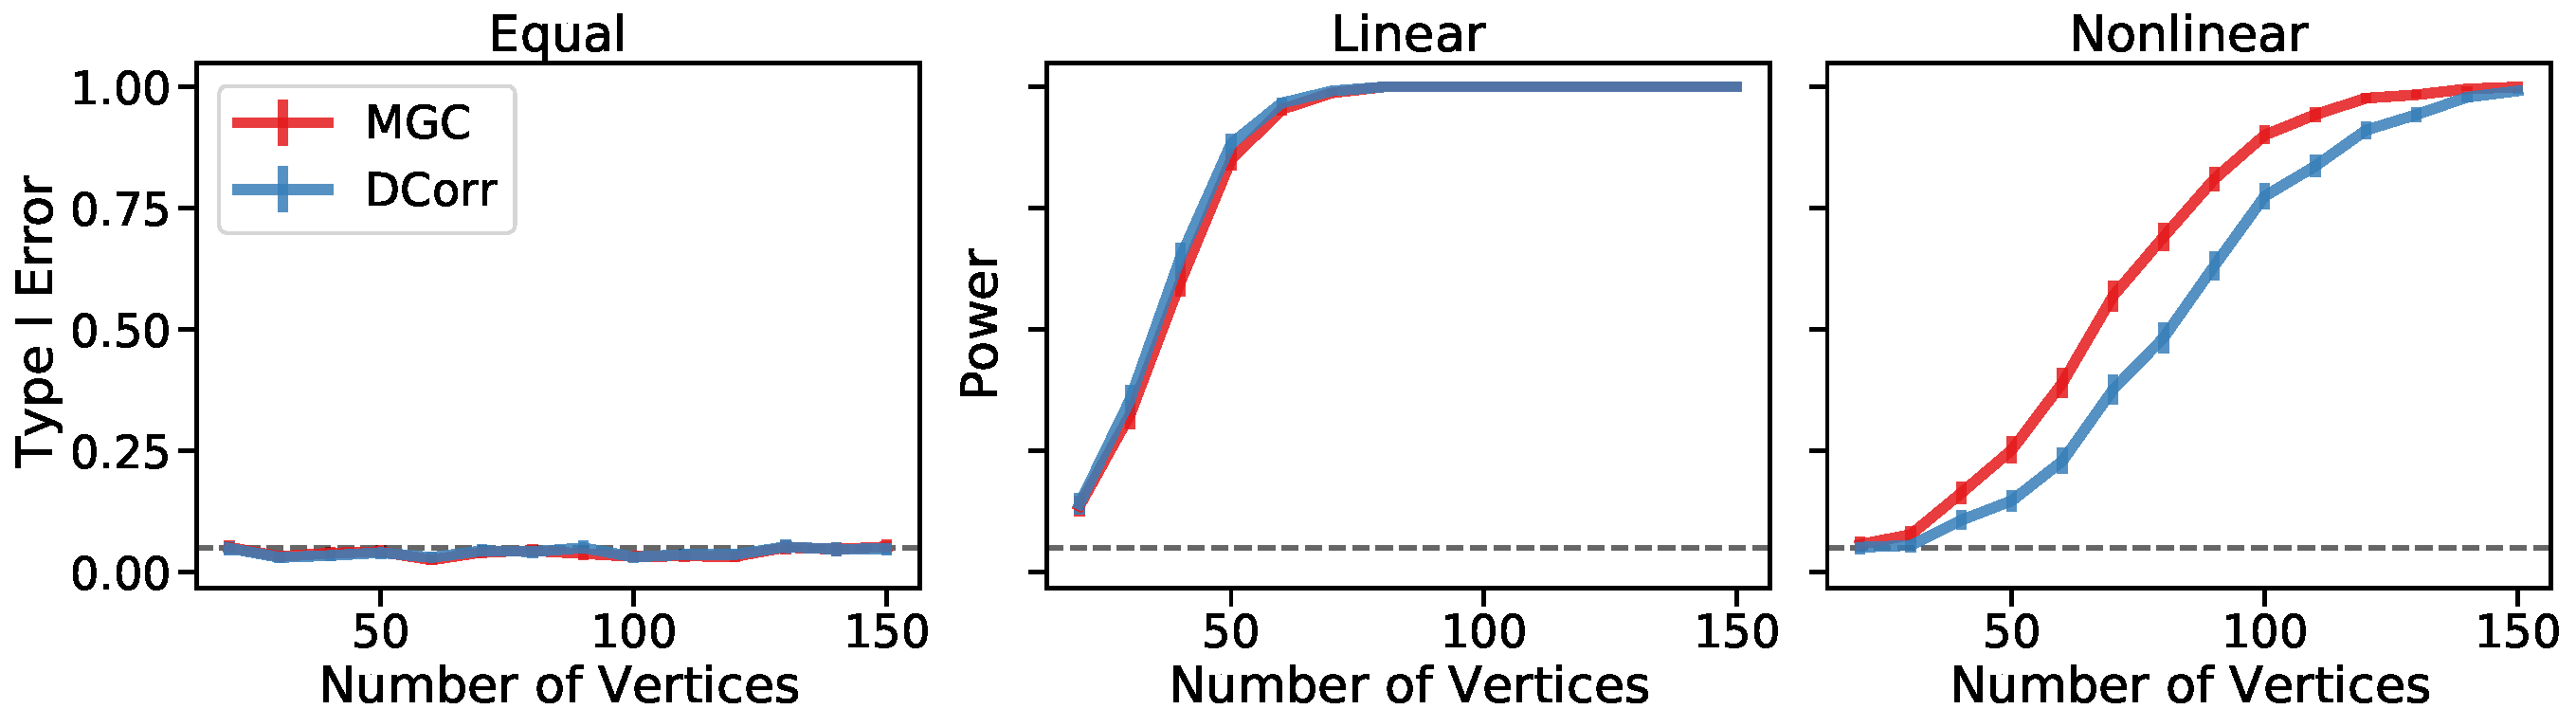
\includegraphics[width=\linewidth]{figures/nonpar/simulations.pdf}
    \caption
    [Type I error and power vs. number of vertices ($n$) for detecting differences in the distribution of latent positions using different methods (DCorr and MGC).]
    {Type I error and power vs. number of vertices ($n$) for detecting differences in the distribution of latent positions using different methods (DCorr and MGC). Dashed lines represent $\alpha=0.05$, and error bars represent $95\%$ confidence interval.
    \textit{(Left)} When the distributions of the latent positions are identical, both methods are valid as power is near or at $\alpha=0.05$. \textit{(Middle)} When the distributions are linearly dependent, both methods are equally powerful and consistent. \textit{(Right)} When the distributions are nonlinearly dependent, both methods are consistent, but MGC is more powerful than DCorr.}
    \label{fig:simulations_nonpar}
    % TODO figure captions always must say n & p, and refer to text where simulations are described. same comments for fig 2. 
\end{figure}

\section{Synthetic and Real Data Applications}
% In this section, we discuss applications to synthetic and real data using the \textit{Drosophila melanogaster} connectomes. 

\paragraph{\textit{Drosophila melanogaster} brain}
The connectomes, or brain graphs, of the \textit{Drosophila melanogaster} mushroom body was obtained in \cite{eichler2017complete}. The left brain graph ($A^L$) has $n=163$ neurons represented with the vertices, and the right brain graph ($A^R$) has $m=158$ neurons. Both graphs are binary with $A_{i j} \in \{0, 1\}$, symmetric with $A= A^\top$, and hollow with $\text{diag}(A) = \vec 0$. The edges of the data represent whether a synaptic connection exist between a pair of neurons or not.

\paragraph{Synthetic Data Analysis}
The performances of the two SVD alignment methods (median flipping and Optimal Transport Procrustes) and two hypothesis tests (DCorr and MGC) are analyzed by simulating synthetic data from the \textit{Drosophila} connectomes. Given an estimated latent position matrix $\hat X\in \mathbb{R}^{n\times d}$ obtained from one of the hemispheres (either $A^L$ or $A^R$), a pair of new latent position matrices are sampled, either with or without perturbation, to analyze the power and validity of various methods as a function of the number of vertices and the effect size. The latent position matrices, $\hat X$, are multivariate with $d=3$ for both hemispheres, which is given by the likelihood profile of eigenvalues \cite{zhu2006automatic}.

The first step in data generation is to sample with replacement a set of $m$ vertices from the original graph. Let $\mathcal{P}\subseteq [n]$ be the set of indices for the randomly selected vertices, where $|\mathcal{P}|=m$. For each $i\in\mathcal{P}$, a pair of $d$-dimensional random latent positions $Y_i$ and $Z_i$ are independently generated
via 
\[Y_i \sim \mathcal{MVN}(\hat X_i, \hat\Sigma(\hat X_i)), \quad\quad \quad Z_i \sim  \mathcal{MVN}(\hat X_i + \epsilon_i, \hat\Sigma(\hat X_i)),\]
where $\mathcal{MVN}(x, \Sigma)$  is a $d$-variate normal distribution with mean $x$ and covariance $\Sigma$, and $\hat\Sigma(\hat X_i)$ is the covariance matrix of the difference between $\hat{X}_i$ and  $X_i$ given by the central limit theorem in \cite{Athreya2015}, which is introduced to account for the fact that the true latent position $X_i$ is not observed. A random subset $\mathcal{O} \subseteq \mathcal{P}$ of the vertices are perturbed by adding $\epsilon_i$,  defined as 
\begin{align*}
\epsilon_j &\sim 
\begin{cases}
     \text{Unif}(\mathcal{S}^d_r), & \text{if}~j \in \mathcal{O}\\
    \vec 0, & \text{otherwise},\\
\end{cases}
\end{align*}
where $\text{Unif}(\mathcal{S}^d_r)$ is the uniform distribution on the surface of a $d$ dimensional sphere with radius $r$. Thus, $r$ represents the effect size, and $\rho = |\mathcal{O}| / m$ is the proportion of changed vertices. Given the new latent position matrices $Y$ and $Z$, a pair of undirected graphs $A$ and $B$ are generated by sampling the edges independently as $A_{ij}\sim\text{Bernoulli}(\min\{1, \max\{0, Y_i^\top Y_j\}\})$ and $B_{ij}\sim\text{Bernoulli}(\min\{1, \max\{0,Z_i^\top Z_j\}\})$, for $i>j$. $A$ and $B$ are symmetrized by setting $A_{ij} = A_{ji}$ and $B_{ij} = B_{ji}$.
% TODONE that is how we sample the upper triangle, but then we do stuff to make it symmetric, please clarify. 

\begin{figure}[b!]
    \centering
    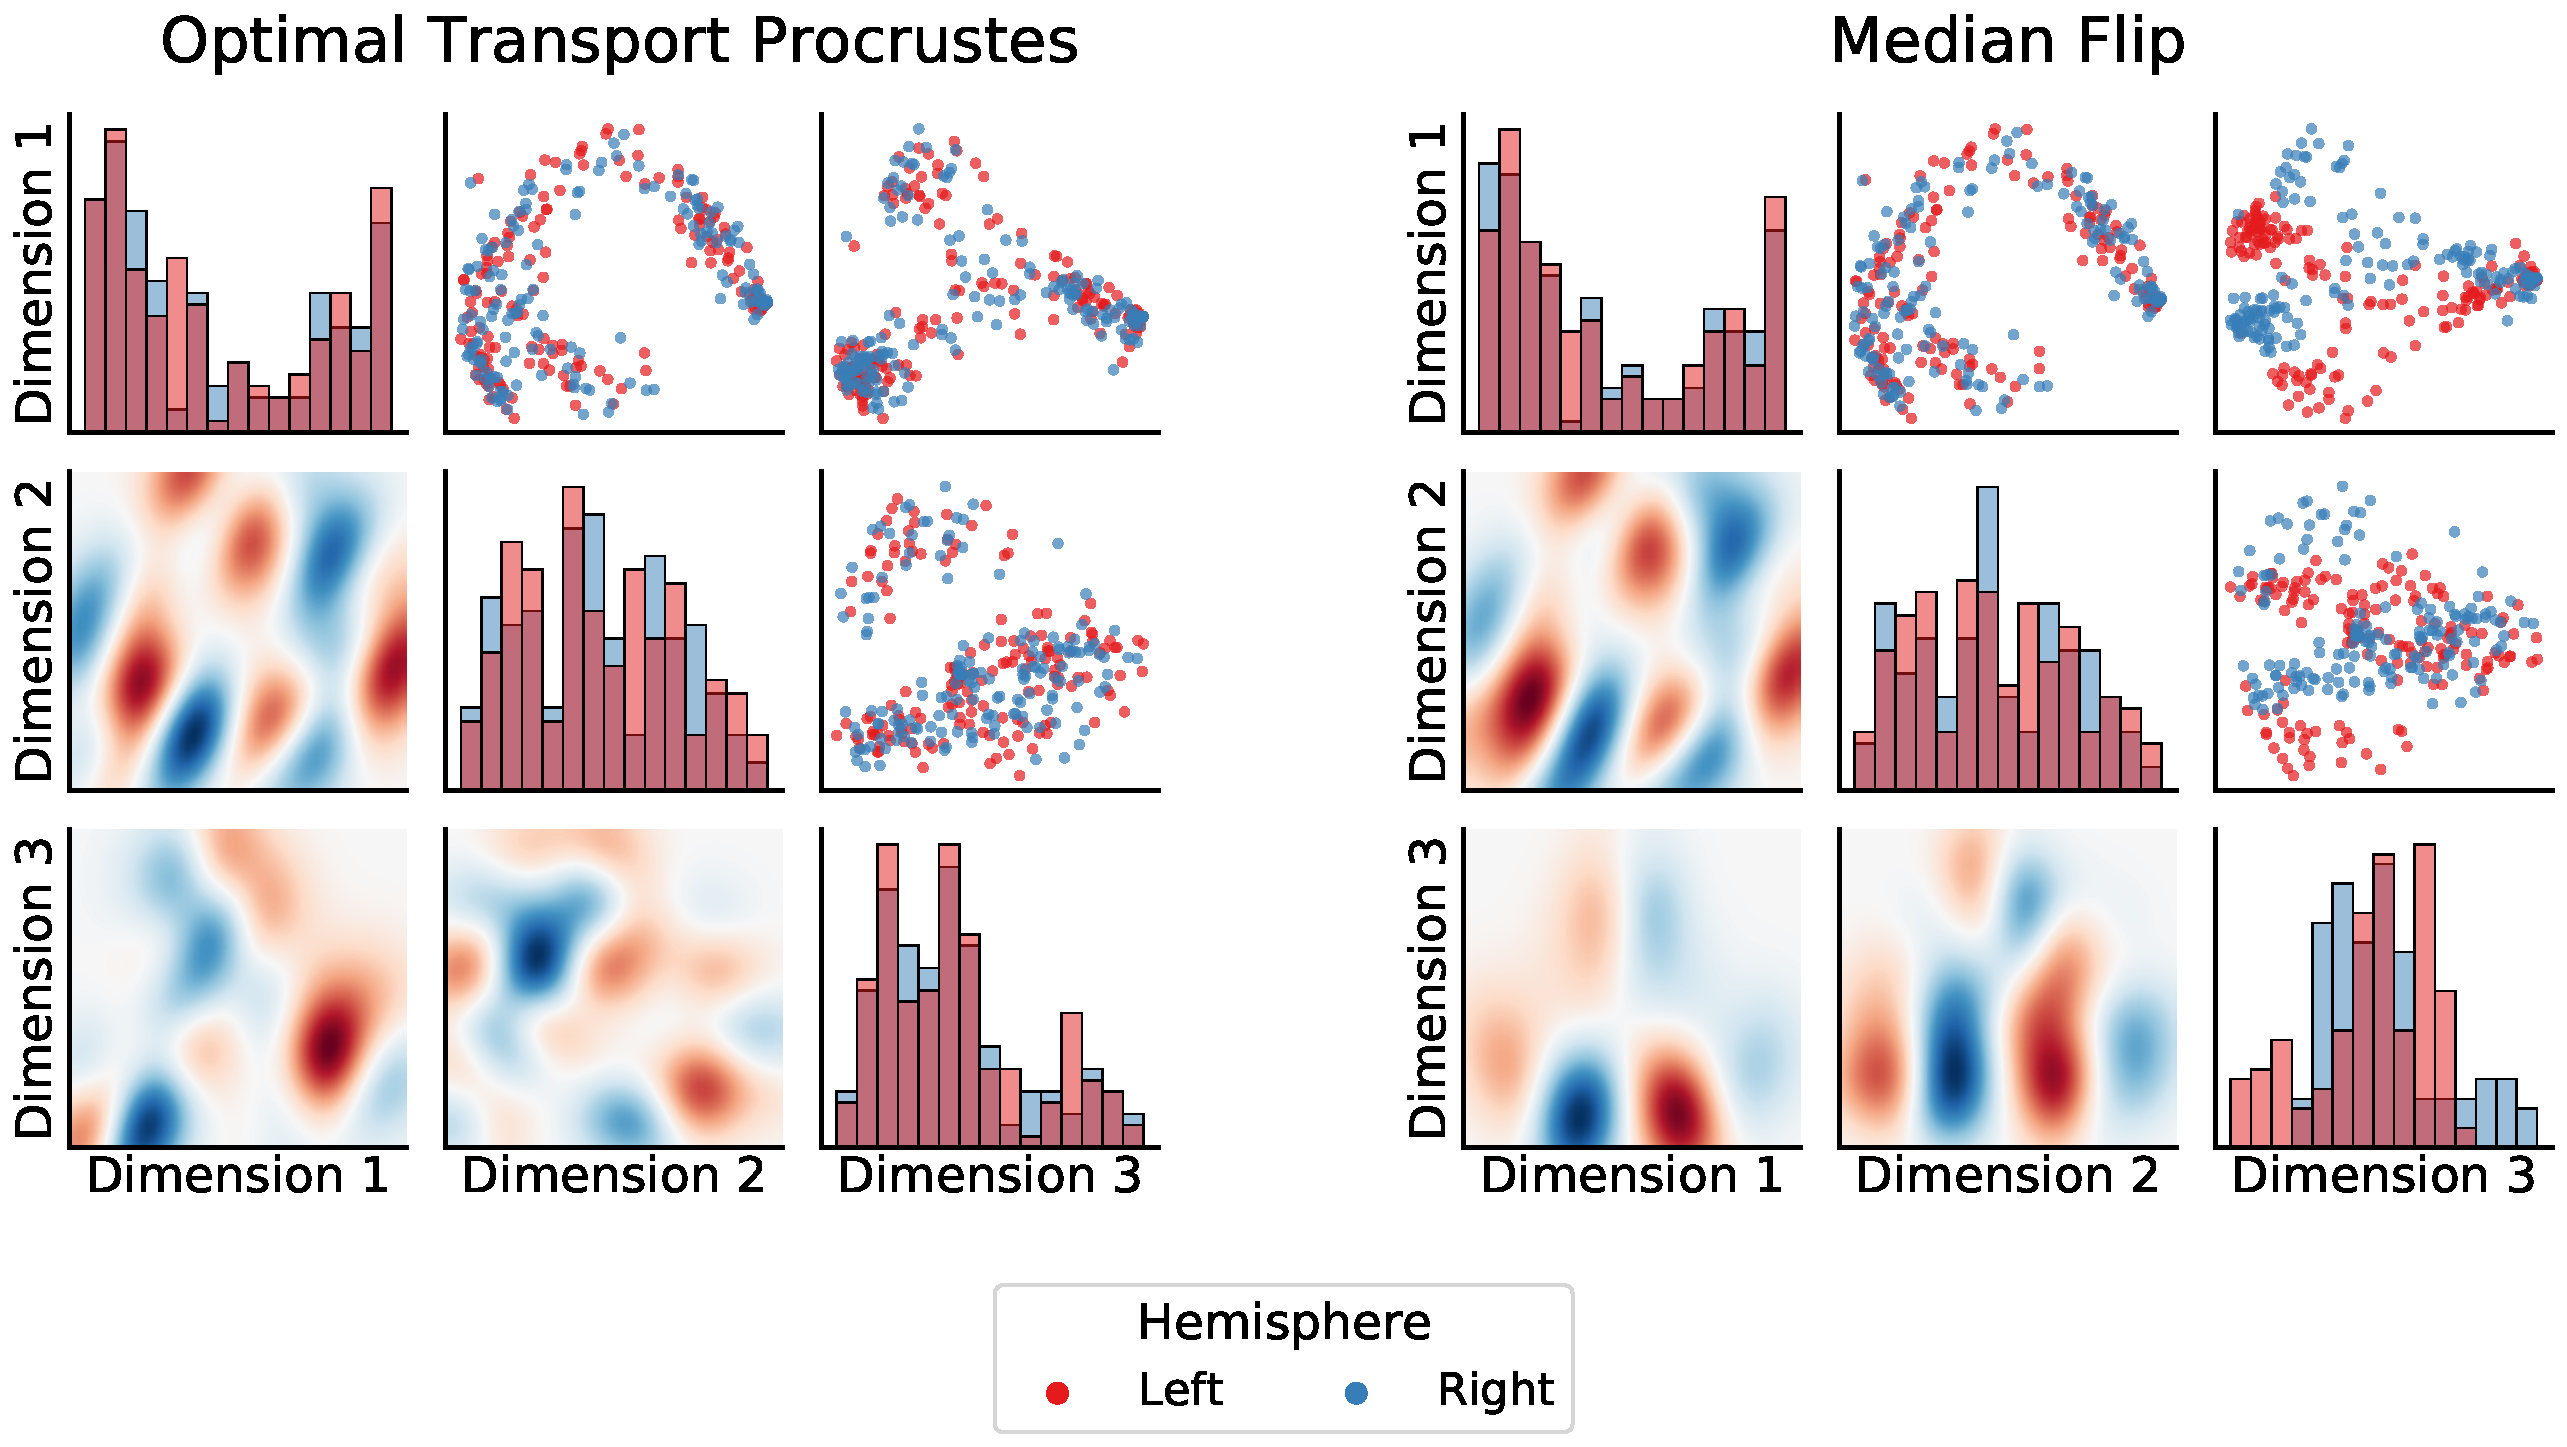
\includegraphics[width=1\linewidth]{figures/nonpar/figure3.pdf}
    \caption[Type I error and power vs. number of vertices ($n$) using synthetic data generated from \textit{Drosophila} connectomes.]
    {Type I error and power vs. number of vertices ($n$) using synthetic data generated from \textit{Drosophila} connectomes. The effect size, or the magnitude of the change in latent positions, is fixed at $r = 1$. The gray dashed line is $\alpha=0.05$.
    Each row represents right or left hemisphere of the brain, and each column represents different proportion of vertices changed. When $\rho = 0$, the latent position distributions $F_V$ and $F_W$ are the same. Latent position alignment via median flip is invalid as shown in first column ($\rho = 0$) as type I error is above $\alpha$ and increasing with the size of the graphs; OTP resolves the invalidity of median flip. 
    Testing via MGC is more powerful than testing via DCorr as shown in columns where $\rho = 0.5$ and $\rho = 1$.
    Curves for median flip testing are omitted in the middle and right panels since using median flip results in an invalid test. 
    }
    \label{fig:synthetic_power}
\end{figure}

Once the new adjacency matrices $A$ and $B$ are sampled, latent positions are estimated with embedding dimension $\hat{d} = 3$, and then we test the hypothesis that the distributions used to generate their latent positions are the same. % via $(V, A)\sim\text{RDPG}_m( F_{V})$ and $(W, B)\sim\text{RDPG}_m( F_{W})$. The hypothesis $H_0: F_{V} = F_{W}$ vs $F_{V} \neq F_{W}$ is tested by estimating the latent positions via ASE then using both alignment methods (median flip and OTP) and test methods (DCorr and MGC). 
The hypotheses are rejected at a significance level $\alpha=0.05$, and the empirical power based on 500 Monte Carlo replicates is reported. This process is repeated for increasing number of vertices with $m\in[20, 200]$, and proportion of changed vertices with $\rho \in \{0, 0.5, 1\}$, while keeping the effect size constant with $r = 1$ for both left and right \textit{Drosophila} mushroom body. The effect size is fixed because there is not enough influence on the power at smaller values of $r$.

Figure \ref{fig:synthetic_power} shows that aligning the latent positions via the median flip yields invalid results for both DCorr and MGC. 
Specifically, when $\rho=0$, both $Y$ and $Z$ are sampled from the same distribution, but both DCorr and MGC yield type I errors  greater than $0.05$ when testing via median flip. 
The OTP alignment resolves the invalidity of the median flip as type I error is near $\alpha = 0.05$ at all sample sizes. 
When $\rho>0$, the empirical power for both DCorr and MGC using OTP increases as the the sample size and proportion of vertices changed increases, showing that both methods are able to identify a significant difference between the distributions.
Lastly, the MGC test statistic is more powerful than the DCorr test statistic in all scenarios where $\rho >0$.


\paragraph{Left vs Right Larval \textit{Drosophila} Mushroom Body}

The left and right \textit{Drosophila} mushroom body are similar, but not identical. To compare  these hemispheres, we test the difference of the distributions of the graph of the left mushroom body ($L$) and the graph of the right mushroom body ($R$).
While the left and right mushroom body connectomes have different number of vertices, we did not correct the embeddings since the difference is small.
The ASE of left and right hemispheres are denoted by $\hat{X}_L$ and $\hat{X}_R$ with assumed distributions $F_L$ and $F_R$, respectively.
We test the hypothesis $H_0: F_L = F_R$ vs $H_1: F_L \neq F_R$ with various embedding dimensions, $\hat d \in \{1, 2, 3, 4, 5\}$. The $p$-values are shown in Table \ref{tab:pvals}.

At lower embedding dimensions ($\hat d \in \{1, 2\}$), testing via median flip and OPT for MGC and DCorr do not reject the null. 
However, at higher embedding dimensions ($\hat d \in \{3, 4, 5\}$), testing via median flip rejects the null, but testing via OPT does not for both MGC and DCorr. 
Figure \ref{fig:drosophila} shows that the estimated latent positions of both hemisphere are similar, suggesting there is no difference in the distributions, but median flip misaligns the third dimension. 
The misalignment causes MGC and DCorr to reject the null. 
Thus, the left and right \textit{Drosophila} mushroom body are not significantly different.


\begin{table}
\centering
\begin{tabular}{llllll}
\toprule
\textbf{Algorithm} &       \multicolumn{5}{c}{\textbf{$p$-value}}      \\
\cmidrule(lr){2-6} 
  &      $\hat d = 1$ &    $\hat d = 2$ &  $\hat d = 3$ & $\hat d = 4$ & $\hat d = 5$ \\
\midrule
MGC+OPT      &  \textcolor{ForestGreen}{0.986} &  \textcolor{ForestGreen}{1} &  \textcolor{ForestGreen}{1} &  \textcolor{ForestGreen}{0.999} &  \textcolor{ForestGreen}{0.952} \\
DCorr+OPT    &  \textcolor{ForestGreen}{0.985} &  \textcolor{ForestGreen}{1} &  \textcolor{ForestGreen}{0.997} &  \textcolor{ForestGreen}{0.998} &  \textcolor{ForestGreen}{0.951} \\
MGC+Median   &  \textcolor{ForestGreen}{0.993} &  \textcolor{ForestGreen}{1} &  \textcolor{Red}{0.001} &  \textcolor{Red}{0.001} &  \textcolor{Red}{0.001} \\
DCorr+Median &  \textcolor{ForestGreen}{0.986} &  \textcolor{ForestGreen}{1} &  \textcolor{Red}{0.005} &  \textcolor{Red}{0.007} &  \textcolor{Red}{0.038} \\
\bottomrule
\end{tabular}
\caption
[P-values from testing for differences in distribution of the left and right \textit{Drosophila} mushroom body, specifically $H_0: F_L = F_R$ vs $H_1: F_L \neq F_R$ at various values of embedding dimension, $\hat d$.]
{P-values from testing for differences in distribution of the left and right \textit{Drosophila} mushroom body, specifically $H_0: F_L = F_R$ vs $H_1: F_L \neq F_R$ at various values of embedding dimension, $\hat d$. With $\alpha=0.05$, testing via optimal transport Procrustes and median flip do not reject the null hypothesis when $\hat d \in \{1, 2\}$. However, when $\hat d \geq 3$, testing via optimal transport Procrustes does not reject the null hypothesis, but testing via median flip does reject the null hypothesis when it should not. The green $p$-values correspond to successful alignment of latent positions, while red $p$-values correspond to misalignment of latent positions.}
\label{tab:pvals}
\end{table}


\begin{figure}[t!]
    \centering
    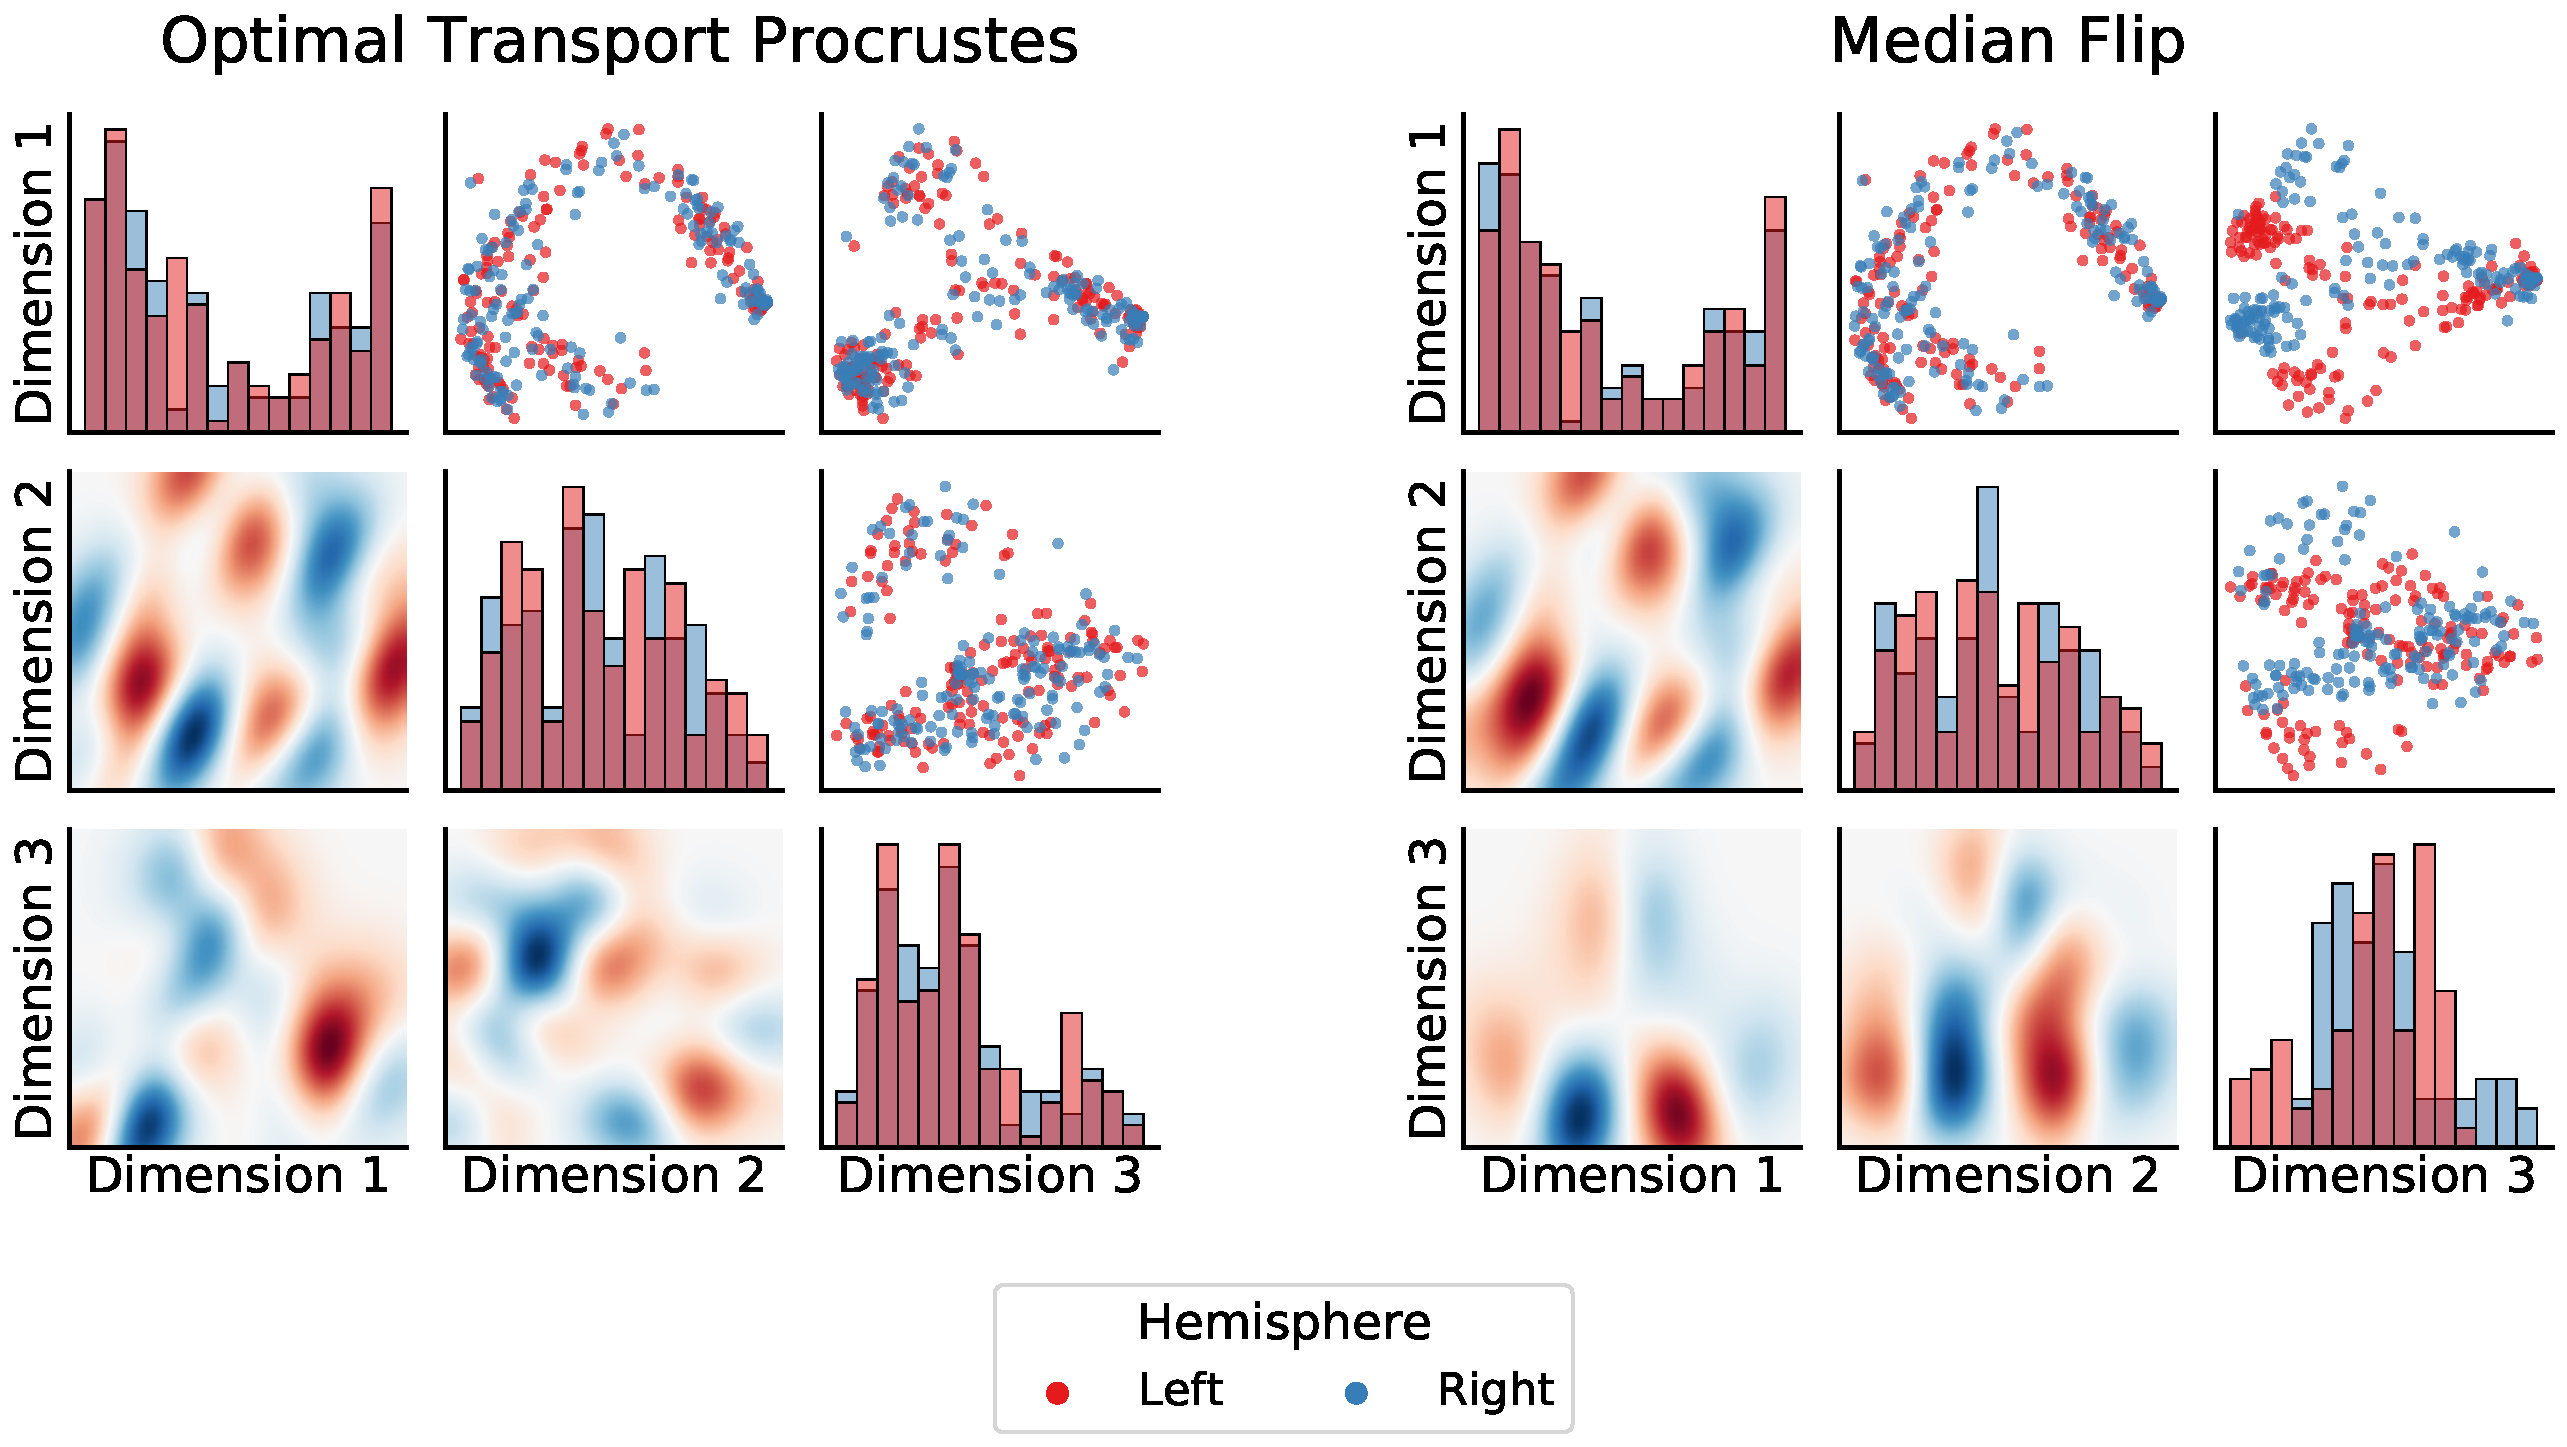
\includegraphics[width=\linewidth]{figures/nonpar/figure3.pdf}
    \caption[Embeddings for the \textit{Drosophila} connectomes after alignment with Optimal Transport Procrustes (left) and median flip (right) with embedding dimension $\hat d =3$]
    {Embeddings for the \textit{Drosophila} connectomes after alignment with Optimal Transport Procrustes (left) and median flip (right) with embedding dimension $\hat d =3$. The diagonals are histograms of each dimension, upper off-diagonals are pairwise scatter plots, and lower off-diagonals are the difference of the kernel density estimates of the two embeddings. 
    \textit{(Left)} OTP properly aligns all three dimensions. 
    \textit{(Right)} Median flips results in misalignment in dimension 3 of the left hemisphere embedding. 
    }
    \label{fig:drosophila}
\end{figure}


\section{Discussion}

The results presented herein demonstrate the improvement of the nonparametric two-sample graph testing presented in \cite{tang2014nonparametric} by aligning estimated latent positions via Optimal Transport Procrustes (OTP) and testing via multiscale graph correlation. For applications in connectomics, we show that the orthogonal nonidentifiabilities that arise from adjacency spectral embedding can significantly impacts the results. Specifically, the synthetic data experiments show that median flip can invalidate DCorr and MGC, but OTP resolves the inadequacy of median flip. Both simulated and synthetic experiments show that MGC is more powerful than DCorr when testing via OTP.  Thus, testing via OTP and MGC is not only more powerful, but also more trustworthy. While this work focuses on cases where the two graphs have the same number of vertices, the testing procedure can be extended to cases where the two networks have different number of vertices by correcting the variance of the estimated latent positions \cite{correcting-nonpar}.


\section{Code}
All code and data used in the analysis are available at \url{https://github.com/neurodata/improving-latent-distribution-test}. 
The analysis were performed using the \texttt{graspologic} (\url{https://github.com/microsoft/graspologic}) and \texttt{hyppo} (\url{https://github.com/neurodata/hyppo})  Python packages  \cite{chung2019graspy, panda2021hyppo}. 
The methods described herein are implemented in \texttt{graspologic}.
 % nonpar
\chapter[The Heritability of Human Connectomes]{The Heritability of Human Connectomes: a Causal Modeling Analysis} \label{chap:heritability}

This chapter documents our investigations into the heritability of structural connectomes in humans. %Importantly, this study approached the heritability problem from a causal perspective and leveraged statistical network models 
This chapter is currently in review at Imaging Neuroscience, and a preprint is available at bioRxiv (DOI: \url{https://doi.org/10.1101/2023.04.02.532875}) and is distributed under the terms of a Creative Commons Attribution License that permits unrestricted use and redistribution provided that the original author and source are credited.

\begin{singlespace}         % you can also use onehalfspace to relax the spacing
    \fullcite{chung2023heritability} \mybibexclude{chung2023heritability}
\end{singlespace} 

\pagebreak
\section*{Abstract}
The heritability of human connectomes - the maps of brain connectivity - is crucial for understanding the influence of genetic and environmental factors on variability in connectomes and their implications for behavior and disease. Unfortunately, current heritability methods can mistake correlation for causation or use models that oversimplify the intricate nature of brain networks, which risks misinterpreting the influence of genetics on brain connectivity patterns. To address these limitations, we propose a new approach that combines causal inference techniques to control for potential confounding with statistical models designed to capture the complex dependencies within brain networks. This allows us to explore more nuanced concepts of connectome heritability by systematically removing shared network structures. Applying our methods to diffusion connectomes derived from the Human Connectome Project, we show that brain connectivity is heritable heritability, even after adjustments for factors like neuroanatomy, age, and sex. However, once we address for common network between connectomes, our causal tests are no longer significant. These results suggest that previous conclusions on connectome heritability may be driven by the shared network structures. Thus, this work highlights the importance for future works to continue to develop data-driven heritability models which faithfully reflect potential confounders and network structures.
\pagebreak


\section{Introduction}
Many common human traits and diseases cluster in families, and are believed to be influenced by several genetic and environmental effects. Heritability quantifies the total variability in a given trait or disease and is attributable to genetic factors and not environmental or stochastic events \cite{tomasetti2015variation}. Thus, heritability is a key factor in predicting disease risk from an individual's history \cite{wray2010genetic}, setting bounds on the ability of genetics to predict disease \cite{wray2010genetic}, providing justifications for further genetic studies, and developing genetic treatments for heritable diseases, such as sickle cell anemia \cite{steinberg2012genetic, xu2021crispr, bennett2018gene, malik2020gene, lukacs2019gene}. 
%There are two main definitions of heritability; narrow-sense heritability $\parens{h^2}$ and broad-sense heritability $\parens{H^2}$ \cite{falconer1996introduction}. Narrow-sense heritability measures only the additive genetic effects, and broad-sense heritability measures all possible genetic effects, such as additive, dominance, and epistasis (i.e. the interaction of multiple genes contributing to a phenotype). In typical human twin studies, narrow-sense heritability is most commonly studied because there is insufficient information to estimate the dominant genetic effects and epistasis.

Numerous methods of estimating heritability, that is, partitioning phenotypic variance into genetic and environmental components, have been applied to various ``simple'' traits in twin studies. The intraclass correlation (ICC) \cite{fisher1992statistical}, which estimates the amount of variation that is common to the group as a proportion of variation in the population, and Falconer's method \cite{falconer1996introduction}, which is the difference in ICC in identical and fraternal twins of a given trait, have been used to show significant heritability in human personalities \cite{gottesman1963heritability, floderus1980assessment, vukasovic2015heritability}, anatomy \cite{russell1998heritability, christian1989heritability, post1997heritability, michalowicz1991twin}, and intelligence \cite{eaves1972insignificance, vernon1989heritability}.
Structural equation models (SEMs) have also been used to estimate the heritability of phenotypically complex diseases such as schizophrenia and Alzheimer's \cite{cannon1998genetic, foote2021genetic}. SEMs, in contrast to ICC,  can incorporate multivariate inputs, account for covariates such as sex and age, incorporate familial relationships such as step siblings and parents, and provide more accurate estimates of heritability \cite{j2017assessing}. Although SEMs are extremely useful in human genetics \cite{neale2013methodology}, they exhibit several limitations. For example, phenotypic data are typically assumed to be normally distributed, which is often violated in complex traits, and phenotypic variance can only be modeled as a linear relationship among its variance components. 

Recent advances in neuroimaging have enabled the investigation of heritability in complex neural traits, particularly brain connectivity \cite{dmri_schizo1, dmri_schizo2, dmri_schizo_overview, dmri_heritability1,Sinclair2015-so}. 
Connectomes, which model functional and/or structural connections between brain regions, provide a powerful framework for representing brain connectivity topology through graph theory \cite{bullmore2009complex, galantucci2017structural, aerts2016brain}. 
% \citet{bohlken2014heritability}, for example, employed SEM using simple graph metrics to study the heritability of white-matter brain network topology in whole-brain structural connectomes, which were derived using diffusion magnetic resonance imaging (dMRI) data. The authors showed that both average path length (APL) and clustering coefficient (CC) were substantially heritable. 
% \citet{reineberg2020genetic} similarly used SEM to study the heritability of cortical network co-activation patterns in whole-brain functional connectomes derived from functional MRI (fMRI) data. The authors observed that the brain's genetic functional network organization is diverse, whereby <5\% of functional links were significantly heritable across both datasets. 
However, these earlier studies faced limitations that can hinder clear interpretations. For instance, conclusions about heritability between network metrics (e.g., average path length vs. clustering coefficient) are obscured by the inherent correlations between these measures  \cite{chung2021statistical}.
% It remains unclear, for instance, how to interpret a finding such as greater heritability of APL relative to CC given that both are highly correlated \cite{chung2021statistical}. 
% Another limitation alludes to open statistical questions at the intersection of graph theory and connectomics -- given that a wide variety graph metrics are available for studying connectomes, how does one select the most appropriate metrics to accurately assess the heritability of brain connectivity, and do so without inflating the risk of false discoveries due to multiple comparisons? Although graph theoretic features are often intuitive and logical descriptors of individual connectomes, no set of graph statistics can fully describe the network topology \cite{chung2021statistical}. Finally, connectomes are inherently non-Euclidean and non-Gaussian data, and current methods, such as SEMs that assume Euclidean and Gaussian data, are inadequate and cannot be applied directly to connectomes. Violating model assumptions can lead to invalid inferences and failure to reproduce. 
Furthermore, the extensive array of graph-theoretical metrics available for connectome analysis raises statistical challenges. Selecting the most appropriate metrics to accurately assess brain connectivity heritability, while mitigating the risk of false discoveries from multiple comparisons, remains an open question. Though graph-theoretical features offer intuitive characterizations of individual connectomes, no single set can fully encapsulates network topology \cite{chung2021statistical}. Finally, the non-Euclidean and non-Gaussian nature of connectome data motivates specialized analytical approaches. Traditional methods like SEMs, which rely on Euclidean and Gaussian assumptions, are inappropriate.  Violating these assumptions risks erroneous inferences and compromises scientific reproducibility.

% In this work, we investigate the heritability of human structural connectomes by framing heritability as a causal question; do changes in genetics cause changes in connectomes?  We first present and define heritability in a causal model, and present a method to detect and estimate heritability based on distance correlations, which measures linear and non-linear dependence between genetics and connectomes (Figure \ref{fig:framework}). We then define three models for comparing connectomes based on the statistical modeling of connectomes, which considers the inherent structure and dependencies within networks. Moreover, by explicitly stating the model assumptions, we reveal several possible notions of connectome heritability. For example, we remove common structures with increasing complexity across connectomes and test whether heritability exists beyond these commonalities. Using data from the Human Connectome Project, we demonstrate that structural connectomes are indeed heritable, even after accounting for observed confounding (e.g. age, neuroanatomy, sex). Following the proposed methodology, our findings provide much needed groundwork for future investigations studying the effects of distal genetic influences on complex neurophenotypic traits. Furthermore, our study underscores the importance of considering the inherent structure and dependencies within networks when assessing heritability, as well as the need for methods that can account for non-Euclidean and non-Gaussian data.
In this work, we frame the question of human structural connectome heritability as a causal inference problem: do genetic changes directly influence connectome variations? To address this, we introduce a causal framework for defining connectome heritability and propose a novel method using distance correlations to detect and estimate this heritability. This approach accommodates both linear and non-linear dependencies between genetics and connectomes (Figure \ref{fig:framework}). Furthermore, we offer three models for connectome comparison, each with distinct assumptions that reveal different potential aspects of heritability. These models systematically remove common network structures with increasing complexity, allowing us to isolate heritable effects beyond these shared patterns. 

Using Human Connectome Project data, we demonstrate that structural connectomes are indeed heritable only up to some connectome model commonalities, even when rigorously controlling for potential confounders (e.g., age, neuroanatomy, sex) 
%TODO add sentence about it disappearing after controlling for structures
Our methodology lays the foundation for future research on how genetic factors influence complex brain phenotypes. Crucially, it highlights the importance of modeling the inherent structure of connectomes and the need for specialized analytical methods that respect the non-Euclidean and non-Gaussian nature of brain connectivity data.

\begin{figure}%[t!]
  \centering
  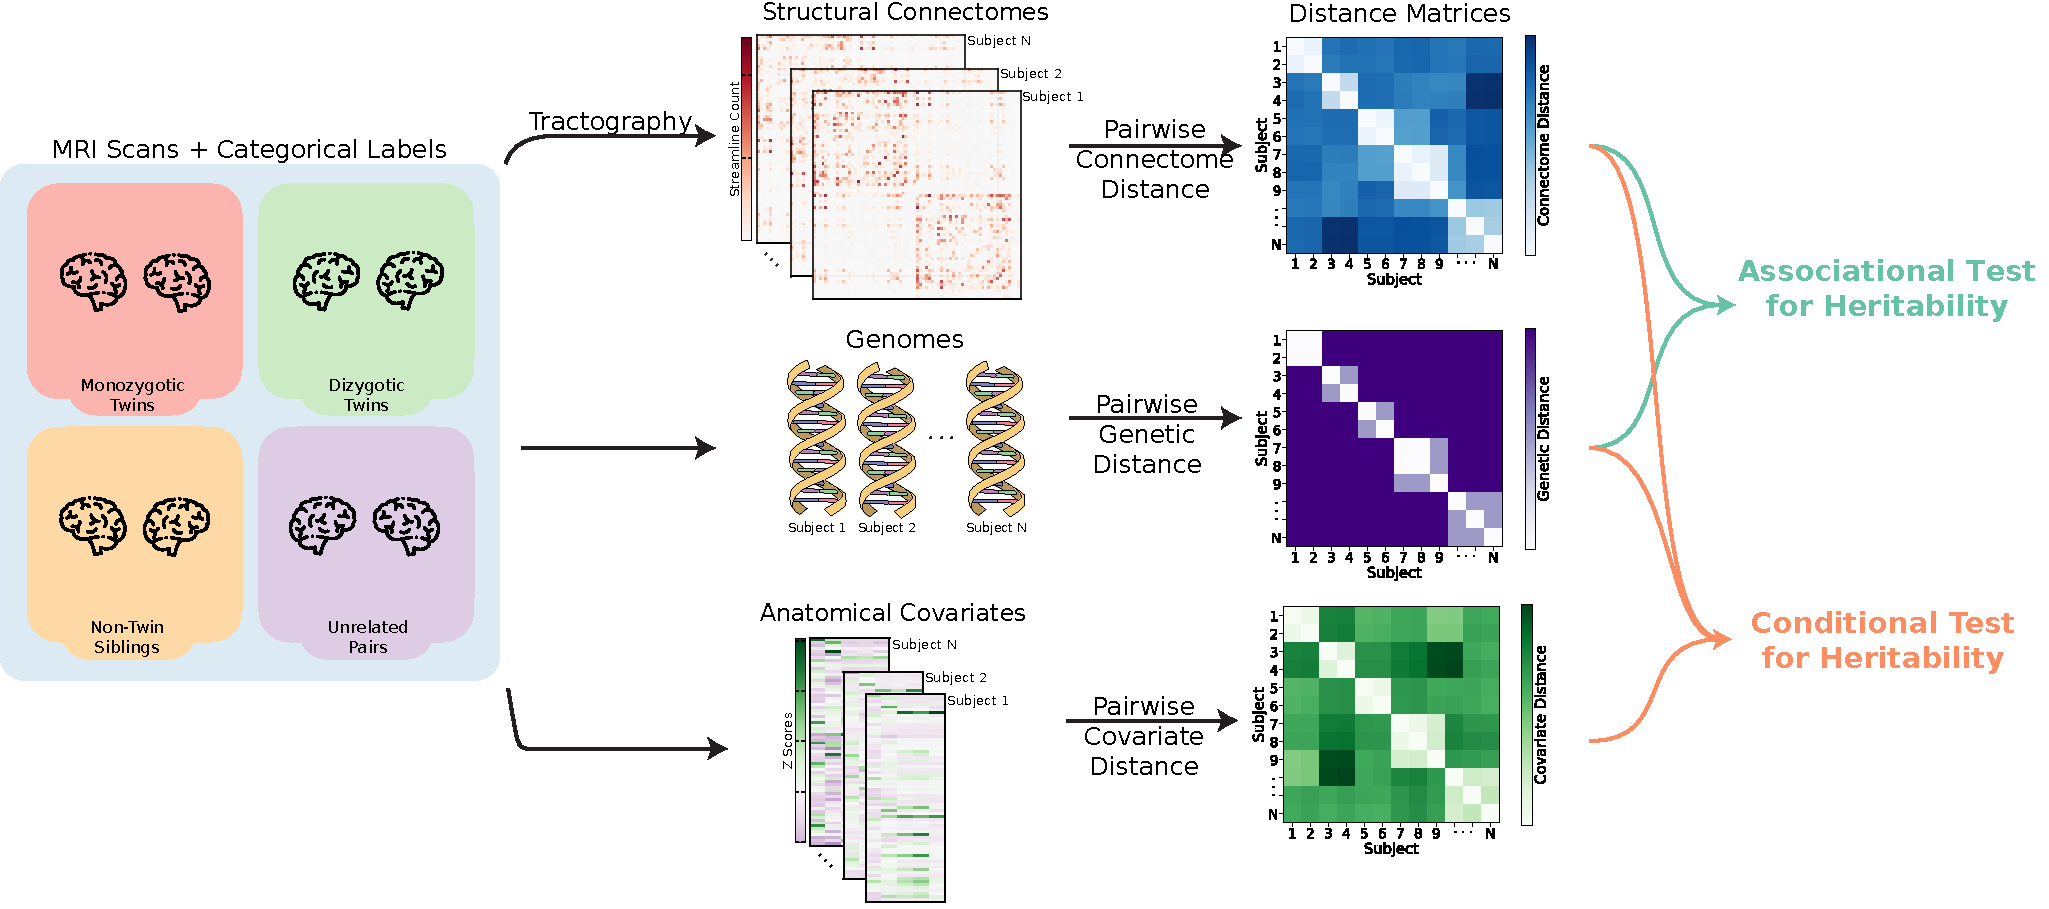
\includegraphics[width=1\linewidth]{figures/herit/framework.pdf}
  \caption{
  \textbf{Overview of the framework for measuring heritability of connectomes.} (\textit{Left}) Diffusion and structural magnetic resonance images (dMRI and sMRI) are processed to generate connectomes. Connectomes are defined on a common set of vertices using brain parcellations. Each pair of individuals has a label corresponding to whether the pair is a monozygotic twin, dizygotic twin, non-twin siblings, or unrelated (e.g. not sharing both mother and father).
  (\textit{Center left}) For each subject, connectomes and covariates are estimated from MRI scans and phenotypic data.
  (\textit{Center right}) For each modality (e.g. connectomes, genomes, and covariates), distances are computed between all possible pairs of subjects using the corresponding distance function. This results in distance matrices that are input to subsequent hypothesis tests.
  (\textit{Right}) Associational effect for connectomic heritability is measured using distance correlation ($\dcorr$). Conditional effect for connectomic heritability is measured using conditional distance correlation ($\cdcorr$). Significance tests provide evidence to reject the null that genomes and connectomes are not related.}
\label{fig:framework}
\end{figure}

\section{Causal Framework for Discovering Heritability in Connectomes} 
\subsection{Heritability in Twin Datasets}
We focus on demonstrating the presence of heritability for structural connectomes in a twin neuroimaging study (see Figure \ref{fig:framework} for an overview). Figure \ref{fig:dag} illustrates a directed acyclic graph (DAG) representing a twin study, where measurements are obtained from individuals across multiple families. In the DAG, the directionality of arrows (e.g. $Z\rightarrow Y$)  indicates a potential causal influence of variable $Z$ on variable $Y$. Ideally, we aim to estimate the causal effect of genetic variation on structural connectome variation while controlling for all possible covariates, observed or unobserved. However, a key limitation is that estimating this pure causal effect is infeasible in practice, as it requires knowledge of both measured and unmeasured confounders.

Given the data available from twin neuroimaging studies, what models can help us provide evidence of heritability?
\begin{enumerate}
    \item \textbf{Associational Heritability:} The simplest model examines whether the genome is associated with connectomes. However, in real studies, both genome and connectomes are often influenced by other covariates. This makes estimated associational effects potentially unreliable, as they may conflate true genetic effects with those of correlated factors. For instance, if brain size relates to both genetics and structural connectomes, we cannot easily distinguish whether observed associations are due to genetics or neuroanatomy.
    \item \textbf{Conditional Heritability:} This model addresses the limitations of associational heritability. It asks whether differences in the outcome (structural connectomes) are associated with differences in genetic exposure, after conditioning on measured covariates. Observing such differences strengthens the argument for causal genetic influence.
\end{enumerate}

Conditional heritability can be considered equivalent to causal heritability under a sufficient condition: the strong ignorability assumption \cite{rosenbaum1983central}.  In twin studies, a simplifying assumption often made is the "equal environment assumption", that monozygotic (MZ) and dizygotic (DZ) twins share environmental factors to a similar degree by virtue of their study design. Additionally, in non-twin siblings, some overlap in covariate distributions is likely (e.g., if siblings share a household). Assuming that other experimental design considerations ensure overlap in covariates such as age, we can posit that neuroanatomy, sex, and age close all possible non-causal pathways that can create spurious correlations (e.g. close potential backdoor paths). If these conditions hold, the conditional heritability in our study can be interpreted as causal. 

% The genome that an individual inherits from his or her parents is the exposure, and the connectomes are the outcomes. We seek to estimate the causal estimand, which is the causal effect of the genome on the connectome. Both measured and unmeasured covariates can introduce confounding biases that affect both the exposure and the outcome. Unmeasured variables that affect the genome, such as race, fall under the category of \textbf{Nature}; unmeasured variables specific to life experiences, including both shared and unshared environmental influences, that affect the connectomes are classified as \textbf{Nurture}. Measured covariates, such as \textbf{Neuroanatomy}, \textbf{Sex}, and \textbf{Age}, also have an impact on the connectomes. 

\begin{figure}
\centering
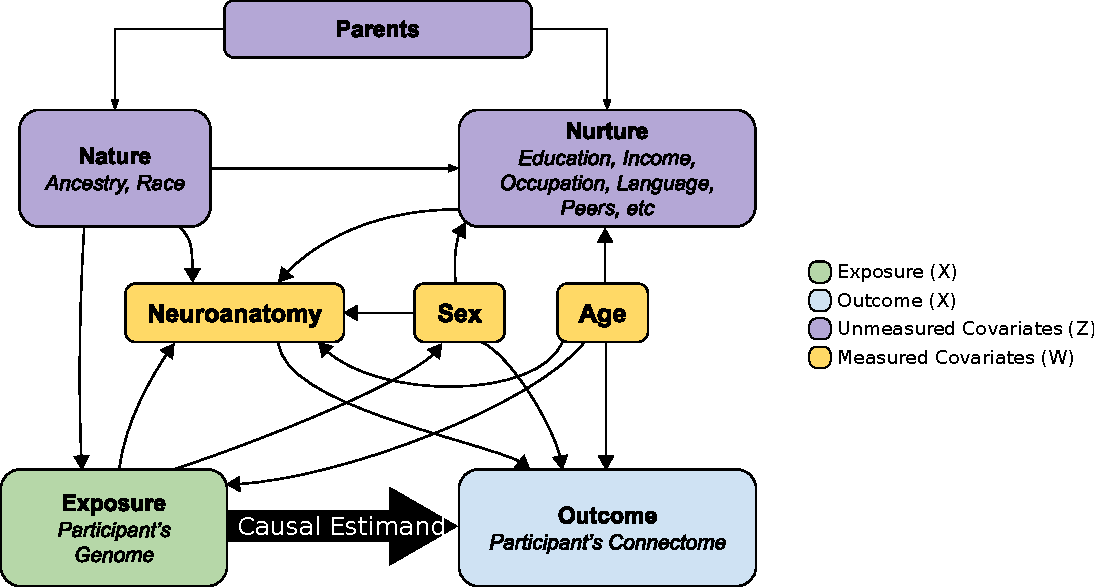
\includegraphics[width=0.8\linewidth]{figures/herit/dag.pdf}
\caption
[Causal Graph of Study Covariates.]
{\textbf{Causal Graph of Study Covariates.} Causal directed acyclic graph (DAG) presents a visual representation of the potential relationships between the genome and connectome, in the context of a twin study. The descriptions depict the various attributes that may be considered as exposures, outcomes, and covariates in such a study. In the absence of confounding, associational effects can be considered as causal effects. However, conditional effects can only be considered as causal when the covariates measured are sufficient to close all backdoor paths.}
\label{fig:dag}
\end{figure}

% The first step in \dcorr\ and \cdcorr\ is to compute the distance matrices, which encode the distances between all pairs of observations. Figure \ref{fig:framework} \textit{(center right)} shows examples of connectome and genome distance matrices. However, computing distances between connectomes is not straightforward because connectomes are high-dimensional and non-Euclidean data. In the following section, we present models and methods of computing distances between a pair of connectomes. 

\subsection{Twin Dataset for Discovering Connectomic Heritability}
We used an open access human brain diffusion (dMRI) and structural magnetic resonance imaging (sMRI) data set from the Human Connectome Project (HCP) Young Adult study, acquired by Washington University in St. Louis (WUSTL) and the University of Minnesota (Minn) \cite{hcp1, hcp2}. Out of the 1206 participants, a total of 1024 participant brain images were processed. Families with only one subject were discarded, and half-siblings were discarded. The data set includes 322 ($196$ females; ages $22-36$ years old, mean = $29.6$ and SD = $3.3$) monozygotic twins, $212$ ($125$ females; ages $22-36$ years old, mean = $28.6$ and SD = $3.4$) dizygotic twins, and $490$ ($237$ females; ages $22-37$ years old, mean = $28.3$ and SD = $3.9$) non-twin siblings. Structural connectomes were derived based on various parcellations. See \ref{sec:network_construction} for more details on network construction. Figure \ref{fig:data} shows visualizations of the average connectome and the difference in two most different subjects for the Desikan parcellation. 

\begin{figure}
    \centering
    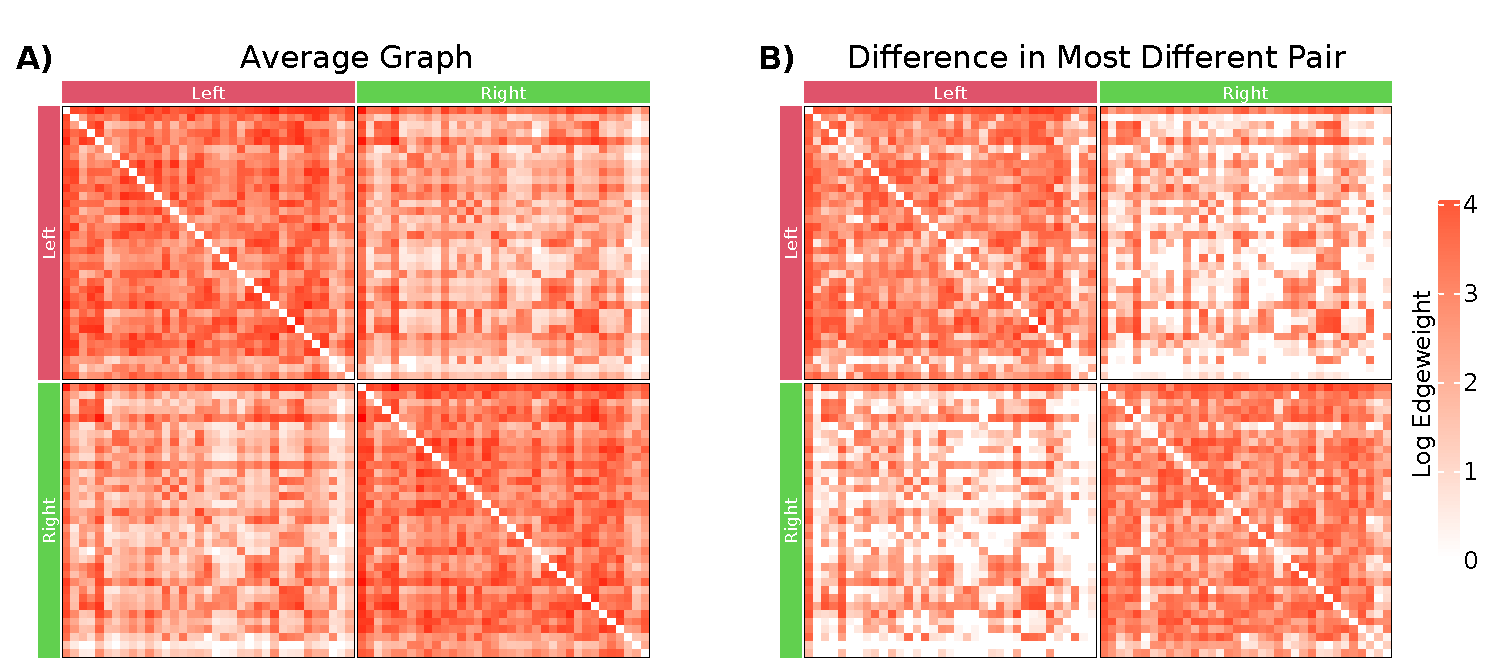
\includegraphics[width=\linewidth]{figures/herit/3-composite.pdf}
    \caption
    [Visualization of connectomes as adjacency matrices using the projected Desikan parcellation with hemispheric labels.]
    {\textbf{Visualization of connectomes as adjacency matrices using the projected Desikan parcellation with hemispheric labels.}  The projected Deskian parcellation was chosen for visualization purposes due to the low number of vertices ($n=70$). 
    \textbf{(A)} Average connectome of all subjects with log-transformed edge weights. 
    \textbf{(B)} Absolute difference of connectomes from the most different pair of subjects with log-transformed edge weights.}
    \label{fig:data}
\end{figure}

\subsection{Illustration of the Value of Statistical Models for Connectomes} \label{sec:heritability_models}
% Sentence about why statistical models for networks
% Dont mention rdpg, but a model where region has an latent vector
% We can estimate these vectors - mention methods for details
% Given these estimates for a pair of connectomes, we have three ways to compute differences between them - mention methods for mathematical details
% mention the three 

1. Networks inherently contain dependencies 
Networks inherently 
(refer to Section \ref{sec:statistical-models} for more details).
The random dot product graph ($\rdpg$) model provides a way to model weighted networks and compute differences between them using statistically principled procedures \cite{Young_Scheinerman_2007, sussman2012consistent, tang2017, tang2017nonparametric}. In this model, a vertex is a region-of-interest (ROI) in the brain, which is represented as a low-dimensional vector called a latent position. The probability of one ROI connecting to another is determined by the dot product of the corresponding latent positions. In other words, a matrix containing the latent positions of all ROIs is a representation of the underlying distribution of the connectome. Given these representations, we propose three different models for computing distances between connectomes (see Section \ref{sec:method-connectome-models} for more details):
\begin{enumerate}[leftmargin=*]
    \item \textbf{Exact model}: This model measures all differences between latent positions, with differences in the latent positions implying differences in the connectomes themselves. Consequently, a hypothesis test based on an exact model aims to test whether there is a correlation between the actual differences in connectomes and the differences in the genomes. 
    \item \textbf{Global model}: This model examines whether the latent positions of one connectome are a scaled version of the other. For example, if the number of edges in male connectomes are consistently larger than those in females, we have no way of differentiating whether significant findings from the exact model are a result of differences in scaling or differences in the fundamental structure of the connectomes themselves. Thus, hypothesis tests based on global model test whether differences in connectomes after adjusting for scaling differences correlate with differences in genomes. The global model assumes that the scaling factor is the same across all regions, meaning that any differences in scaling are not region-specific.
    \item \textbf{Vertex model}: This model is similar to the global model, but it allows for each vertex to be scaled differently. The idea behind this approach is that some vertices may have a greater impact on the overall network than others, so scaling them differently can provide a more accurate representation of the network. Consider the examples of how brain regions connect with each other. Regions in the same hemisphere are more likely to be connected than across hemispheres. Even within the same hemisphere, different regions may have distinct preferences for forming connections with other specific regions. Thus, hypothesis tests based on the vertex model aim to determine whether there are significant differences in connectomes after accounting for differences in vertex-wise scaling. 
    %Note that if the scaling is the same for all vertices, then the {vertex model} is equivalent to the {global model}.
\end{enumerate}

To demonstrate the differences in the connectome models, we simulated connectomes with various latent positions (Figure \ref{fig:simulations}). 
Columns I and II display four pairs of connectomes, each with specific latent position models. Rows (A-C) share the same underlying latent positions, while row (D) has different latent positions. When the connectome model can account for the differences in latent positions between the subjects, we observe a ``uniform'' structure in the differences, with no visible pattern. For the exact model (column III), distances increase as we move down the rows because it cannot account for any scaling, whether global or vertex-wise. We observe patterns in the differences, where red indicates edges in which subject $1$ tended to have more edges, while blue shows edges where subject $1$ tended to have fewer edges. For instance, for each simulation, when subject $1$ tended to have more edges (row B.I-II), we observe uniform red coloring in the differences (row B.III). Similarly, for the global model, we only see patterns in differences when the differences in latent positions are due to vertex scaling, as shown by the gradients of red and blue (C.IV and D.IV). The main takeaway is that any hypothesis tests based on these models can only make claims within the limits of their ability to explain the differences in the pairs of connectomes.

\begin{figure}
    \centering
    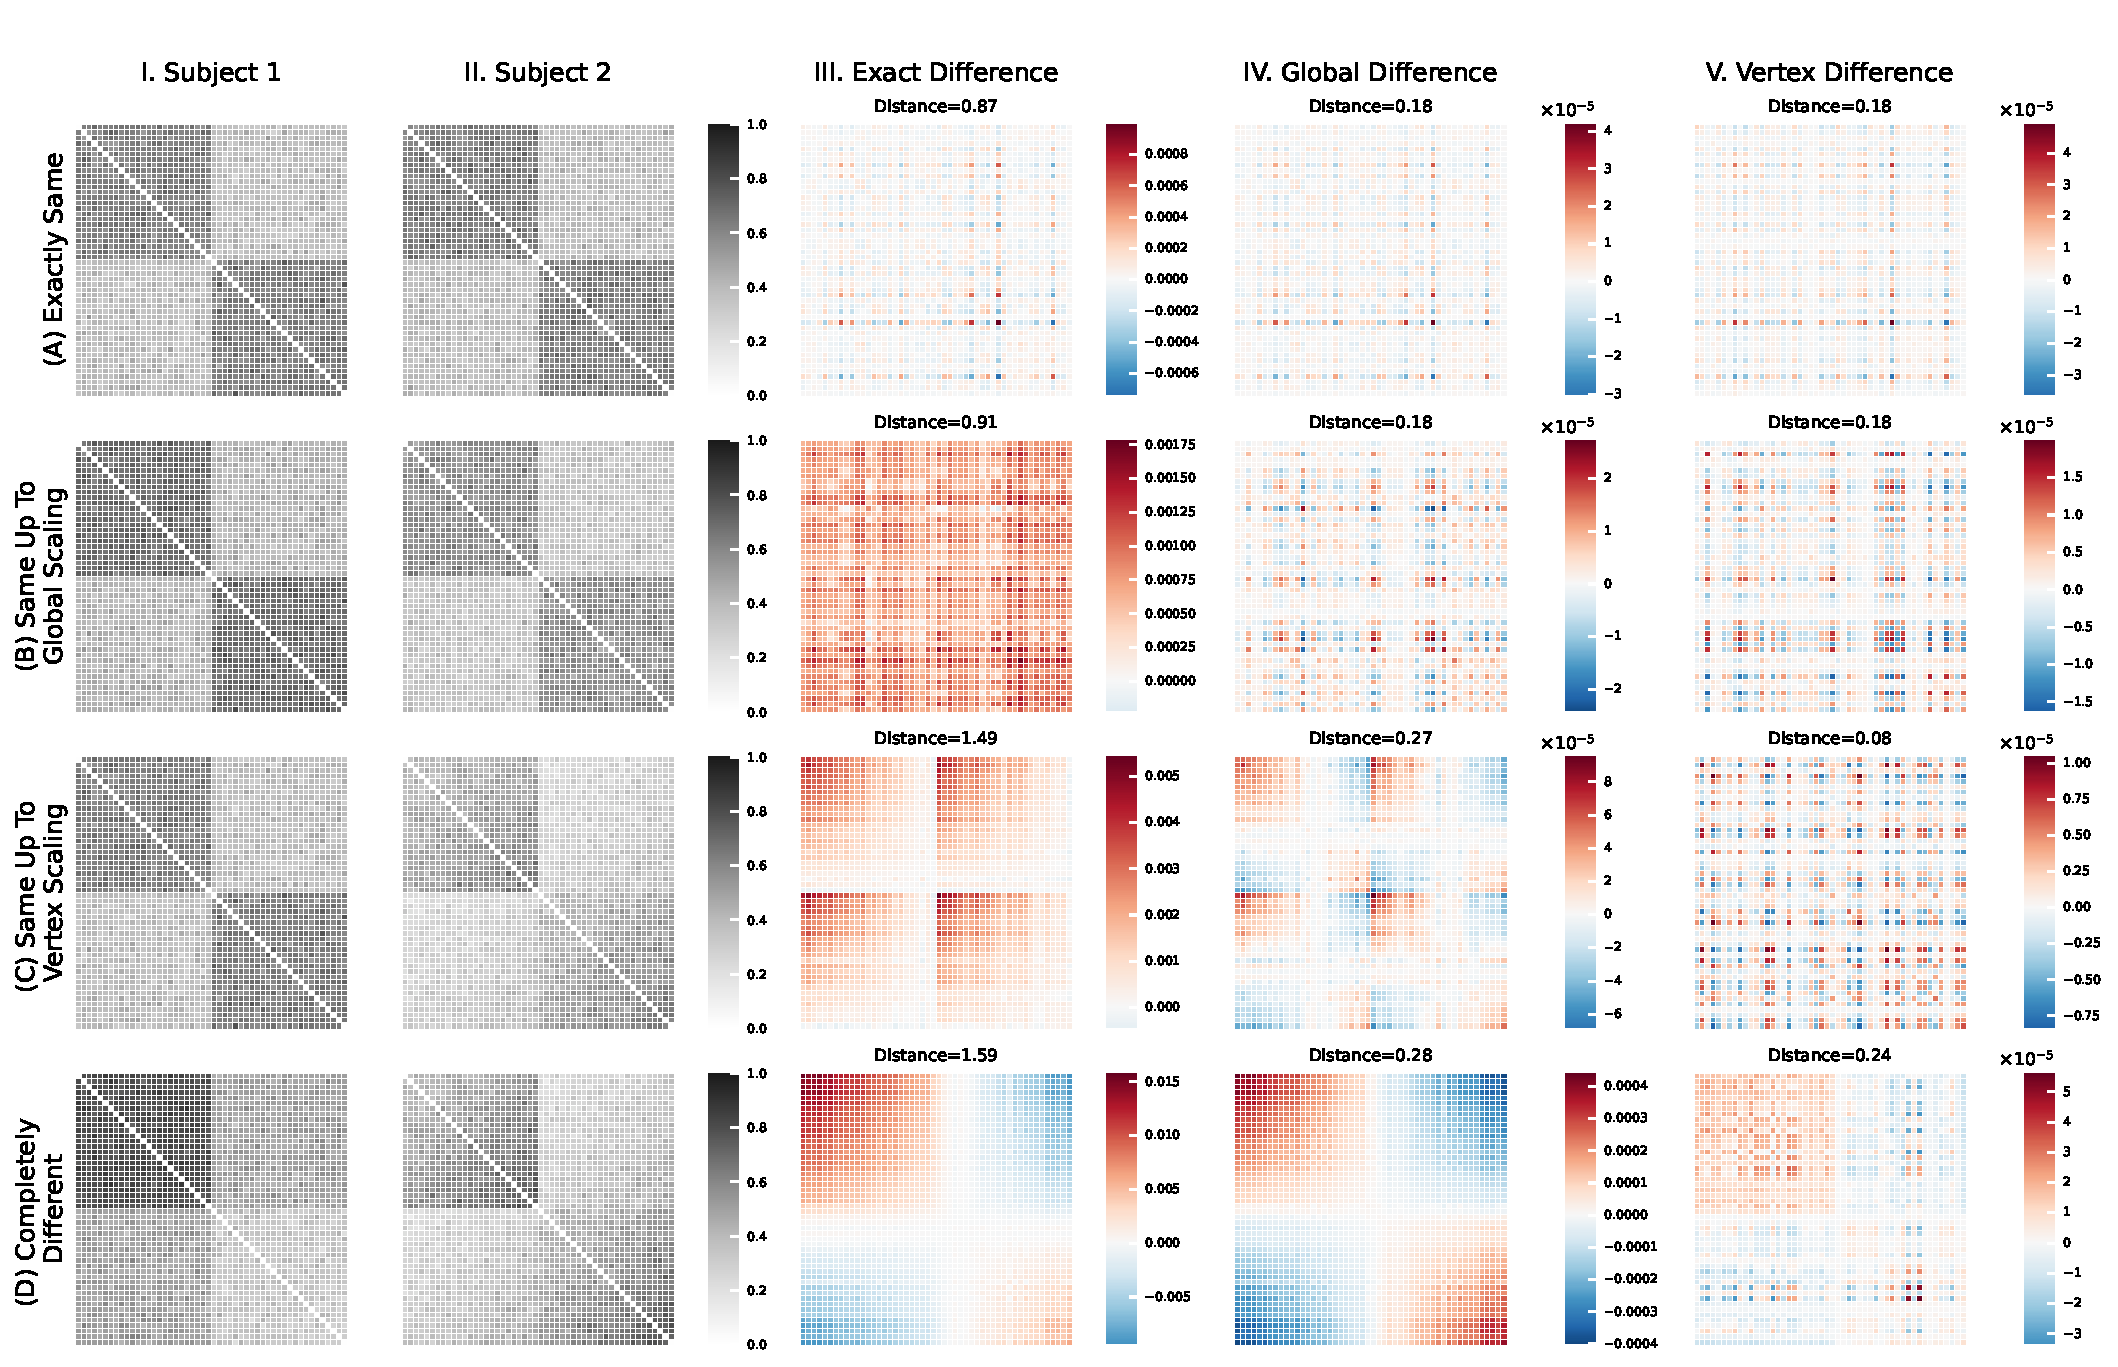
\includegraphics[width=\linewidth]{figures/herit/3-simulations.pdf}
    \caption
    [Simulations demonstrate the utility of connectome models.]
    {\textbf{Simulations demonstrate the utility of connectome models.} Connectomes with $50$ vertices were simulated $100$ times. Columns (I-II) display the average simulated connectomes, while columns {(III-V)} illustrate the differences in latent positions averaged over these simulations. In columns (III-V), red corresponds to when subject $1$ had more edges than subject $2$, while blue corresponds to when subject $1$ had fewer edges. Rows (A-D) correspond to various parameters used to generate the connectomes. Connectomes in rows (A-C) share the same latent positions, subject to scaling transformations, whereas connectomes in row (D) have distinct latent positions, conditional on scaling transformations. When the connectome models accurately represent the generative process, the difference matrix displays a "uniform" structure without discernible patterns (A.III-V, B.IV-V, C.V). However, when connectome models are not appropriate, patterns emerge, as indicated by the increased distance values (B.III, C.III-VI, D.III-V).
    For further technical details of these simulations, see Appendix \ref{sup:simulations}.}
    \label{fig:simulations}
\end{figure} 

\section{Results}

\subsection{Associational Tests for Connectomic Heritability} 

We begin the examination of heritability by first comparing connectomes from monozygotic and same-sex dizygotic twins. By limiting the comparison to these two groups, we minimized the impact of environmental factors (e.g. Nurture in Figure \ref{fig:dag}) on the connectomes and assessed the ability of connectomes to capture variations in the genome. Shared and non-shared environmental influences may arise due to differences in age or sex, which can lead to differences in upbringing or educational experiences. By controlling for such factors, we could reasonably attribute any differences in connectomes to variations in genomes rather than environmental factors. Moreover, if the differences in connectomes between monozygotic twins were ''smaller`` than those between dizygotic twins, it would suggest that connectomes can indeed capture variations in genomes. 
% This would support the idea that variations in the genome can manifest as differences in the connectomes, and thus provide insights into the genetic basis of brain connectivity. 

The distribution of connectome distances is shown in Figure \ref{fig:main-results}A.I-III by the blue and yellow rows, revealing that the medians of monozygotic twins ($N=127$) are smaller than those of same-sex dizygotic twins ($N=75$) for all three connectome models. To determine the significance of this difference, we perform a test for an associational effect using $\dcorr$, yielding $p <10^{-3}$ for all models (Figure \ref{fig:main-results}B.I). These results provide our first evidence for the heritability of connectomes. We then expanded our examination to include non-twin siblings and unrelated subjects (Figure \ref{fig:main-results}A.I-III green and red rows) and observed that the medians grow larger as the familial relationships grow distant. Based on these observations, we tested for associational heritability across all familial relationships, yielding p-values of $<1\times 10^{-3}$ for males and females under all three heritability models (Figure \ref{fig:main-results}B.II). All of these tests indicate a strong associational effect of the genome on connectomes.

\begin{figure}[htp]
\centering
\includegraphics[width=\linewidth]{figures/herit/Desikan-composite.pdf}
\caption
[Testing associational and causal effect of genome on connectomes and neuroanatomy.]
{\textbf{Testing associational and causal effect of genome on connectomes and neuroanatomy.}
\textbf{(A)} Each point represents the pairwise distance between pairs of participants; diamond markers represent the median distance, colors are familial relationships, and rows are sex. 
\textbf{(A.i-iii)} The median distances revealed that MZ twins exhibited smaller distances compared to DZ twins, siblings, and unrelated pairs, whereas the unrelated pairs showed larger distances. DZ twins displayed smaller distances compared to siblings and unrelated pairs, but larger than those of MZ twins. These findings provide qualitative evidence of heritability of connectomes. 
\textbf{(A.iv)} The median distances of neuroanatomy also show qualitative evidence of heritability. 
\textbf{(B)} Colors of heatmaps represent p-values, rows are gender groups, and columns are connectome models. (B.I-II) Associational test for connectome heritability. In (B.I), we only compare MZ and DZ twins, and the significance tests provide evidence of heritability as shown in (A.I-III). In (B.II), we conduct tests across all three familial relationships and observe significant effects, providing further evidence for connectomic heritability. In contrast, in (B.III), we observe significant effects for neuroanatomy, suggesting that the results in (B.I-II) may be confounded by an effect mediator. Subsequently, in (B.IV-V), we perform causal tests for connectome heritability. In (B.IV), we observe significant results only for the exact and global models, indicating that the connectomes remain heritable even after conditioning on the anatomical covariates, age, and sex. This suggests that the results in (B.I-II) cannot be entirely explained by neuroanatomy. The non-significant tests using the vertex model suggest that when we control for covariates and vertex-wise scaling, we can no longer detect heritability. In (B.V), we define a non-heritable subgraph as a collection of vertices that are not heritable by the causal test. We still observe several significant tests, suggesting heritability remains even after discarding vertices.
} 
\label{fig:main-results}
\end{figure}
 
\subsection{Associational Test for Neuroanatomic Heritability} \label{sec:neuroanatomy-dcorr}
Multiple studies have investigated the heritability of human brain anatomy \cite{blokland2012genetic, ge2016multidimensional, brouwer2014heritability, thompson2001genetic, lee2016partitioning, den2013heritability}. 
Structural MRI studies on adults have shown that genetic and environmental factors have a significant impact on brain properties such as volume, shape, and both cortical and subcortical structures.  This suggests that neuroanatomy could be an effect mediator (Figure \ref{fig:dag}).
 To assess if neuroanatomy could be a mediator, several features such as brain volume, axial diffusivity (AD), radial diffusivity (RD), and fractional anisotropy (FA) were computed for each region of the brain. Refer to Section \ref{methods:covariates} for more details. 

We used $\dcorr$~to test for the associational effect of the genome on anatomical covariates. This test assumes that if the covariates and genetics are independent, then brain anatomy is not heritable and has no effect on connectomes. Conversely, if the alternative is true, the associational effects of heritability of connectomes may be partially explained by the heritability of the anatomy itself, making the brain anatomy an effect mediator. Figure \ref{fig:main-results}A.IV illustrates that similar to connectome distances, the median distances increase as familial relationships become more distant. Furthermore, we find that the tests showed $p<10^{-3}$ for all three gender groups under all three connectome models (Figure \ref{fig:main-results}B.III). The significance suggest that the associational heritability of connectomes may partly be due to the effect of anatomy on connectomes. 

\subsection{Causal test for connectomic heritability}
\label{sec:conditional_dcorr}
To account for the dependence of neuroanatomy on genetics, we utilized conditional distance correlation ($\cdcorr$) to estimate the conditional effect of genome on connectomes (Eq. \ref{eq:conditional-hypothesis}). The covariate set also included age, which is a confounder. 
% If the null hypothesis result implies that similarities in brain connectivity are completely explained by similarities in brain anatomy and age, whereas a significant result suggests that the connectomes contain information on brain connectivity beyond anatomy and age, which is still heritable. 
Our results showed $p<10^{-2}$ for exact and global models, but showed $p>.1$ for the vertex model. This indicates that while connectomes are heritable and not entirely influenced by anatomy and age, there is no significant underlying structure beyond the vertex-wise scaling. This contrasts with the results shown in Figure \ref{fig:main-results}B.I-II, highlighting the importance of causal modeling in this study.

\subsection{Non-heritable Subgraphs are also Heritable} \label{sec:subgraphs}
In this section, we consider the possibility that heritability effects detected in Section \ref{sec:conditional_dcorr} are driven by a subset of vertices rather than the entire connectome. That is, it is possible that the connectivity of a subset of brain regions may be highly similar in twins but highly different in non-twin siblings or unrelated individuals. To investigate this, we test for causal heritability by examining the \textit{non-heritable subgraphs}, which are subgraphs induced by the vertices in which no heritable effect can be detected. See Section \ref{sec:cond-effect-vert} for more details on the hypothesis.

The outcomes presented in Figure \ref{fig:main-results}B.V display significant p-values for both the exact and global models across all genders, with only the exact model presenting significant p-values in males. These results suggest that for females, heritability can be fully accounted for by the heritable vertices, while in males, the non-heritable vertices still demonstrate heritability. Nevertheless, when controlling for scaling, the significance observed in the exact model for males is eliminated, indicating that differences in the scaling of the subgraphs explain the observed significance. These findings suggest the presence of an underlying structure in the non-heritable subgraph that cannot be detected at the level of individual vertices and highlights the necessity of statistical modeling of networks.
\section{Discussion} 
\subsection{Summary} \label{discussion:summary}
In this study, we presented the first examination of the heritability of human connectomes using causal modeling and statistical modeling of connectomes. Our investigations into the heritability of connectomes provides strong evidence that the structural connectivity patterns within them are highly influenced by genetics by leveraging causal models and developing a test procedure to detect heritability. To establish this, we first compared the connectomes of monozygotic twins with same-sex dizygotic twins, which allowed us to account for shared environmental factors. Our results demonstrated that not only are connectomes reliable and meaningful, but they are also significantly influenced by genetics. We then extended our analysis to include monozygotic, dizygotic, and non-twin siblings, which further confirmed that connectomes are heritable. However, these results may be confounded by both observed and unobserved covariates. Therefore, we define a set of covariates, which we believe can account for all possible other unobserved covariates. Given this, we found that connectomes remained heritable even after controlling for age and the mediating effect of neuroanatomy. Finally, we demonstrated that the subgraphs formed by sets of brain regions that are not heritable within connectomes are also heritable. This suggests that there is an underlying structure within these subgraphs that is not evident in individual vertices. 
%By uncovering the heritable nature of connectomes, our findings contribute to the broader understanding of genetic influences on brain connectivity and could potentially aid in uncovering new insights into the genetic basis of neurological disorders and cognitive traits.

A key innovation in this study is the utilization of statistical models, specifically the random dot product graphs, for connectomes, which introduces a new representation called latent positions. The models allow us to compare connectomes in various ways and explore different aspects of heritability. The simplest model we use is the exact model, which assesses any differences in the latent positions of connectomes. The global model, on the other hand, accounts for the possibility that connectomes may have different scales, such as variations in edge weights or more connections in general. Therefore, this model quantifies the differences in latent positions after removing the effect of global scaling. The vertex model allows for both global and vertex-wise scaling, enabling the three models to account for increasingly complex structures in connectomes as we move from the exact model to the vertex model. Our findings, as presented in Section \ref{sec:conditional_dcorr}, indicate that genetics play a crucial role in the differences of vertex scaling. However, when addressing vertex scaling of connectomes, heritability becomes undetectable, suggesting that heritability is only due to vertex scaling and not other underlying structures present in the connectomes. These results imply that previous conclusions on connectomic heritability may be influenced by vertex scaling and emphasize the need for further research into the relationship between vertex scaling in RDPG and network statistics, such as clustering coefficients and average path lengths.

There are several other open questions and opportunities for future research on the heritability of connectomes. One potential direction involves studying heritability in different neuroimaging modalities. Although our focus was on human connectomes estimated from diffusion MRI, the methods presented here can be applied to study heritability in connectomes obtained from other modalities, such as functional MRI, magnetoencephalography (MEG), and electroencephalography (EEG), or even in other species, like mice. Another potential direction is incorporating more detailed genetic data, including GWAS, to identify specific genetic variants associated with brain connectivity patterns. This would enable more direct and meaningful comparisons of genomes between subjects and could be readily integrated into the testing procedure presented here.

The findings on heritability in connectome analysis have significant implications for understanding the genetic basis of various neurological and psychiatric disorders. Disruptions in brain connectivity have been implicated in numerous conditions, such as autism spectrum disorder, schizophrenia, and Alzheimer's disease \cite{van2019cross, fornito2015connectomics}. By revealing the heritable components of brain connectivity, researchers can start to pinpoint specific genetic factors that contribute to the development of these disorders. This knowledge could inform the creation of novel diagnostic tools, treatment strategies, and targeted interventions, ultimately enhancing the prognosis and quality of life for individuals affected by these disorders.

% Our main contribution is introducing a novel way to conceptualize heritability as causal effects.  and proposing non-parametric tests to quantify it. Moreover, we employ statistical models for connectomes that introduce a new representation of connectomes called latent positions. This representation enables us to compare connectomes in different ways, resulting in various notions of heritability. The simplest model we use is the exact model, which assesses any differences in the latent positions of connectomes. The global model, on the other hand, accounts for the possibility that connectomes may have different scales, such as variations in edge weights or more connections in general. Therefore, this model quantifies the differences in latent positions after removing the effect of global scaling. The vertex model allows for both global and vertex-wise scaling, enabling the three models to account for increasingly complex structures in connectomes as we move from the exact model to the vertex model.

\subsection{Limitations} \label{discussion:limitations}
\subsubsection{Estimating Heritability}
Heritability is typically defined as the relative contribution of genetic variations as opposed to environmental variations in phenotypic traits, and tests whether the heritability estimate is statistically significant, meaning if heritability exists or not. Numerous methods have been developed to partition phenotypic variation into genetic and environmental components, including techniques such as structural equation modeling (SEM). However, the causal approach presented in this study is distinct from these methods, as it does not aim to estimate heritability in a quantitative manner. Instead, our approach focuses on identifying the presence or absence of heritability by examining causal relationships between genetic factors and phenotypic traits.

The causal approach presented in this study offers a complementary perspective that can contribute to resolving the missing heritability problem. The missing heritability problem arises when the estimated heritability from genetic markers, such as those identified in genome-wide association studies (GWAS), accounts for only a small fraction of the heritability inferred from twin studies using SEMs or similar methods. This discrepancy between the observed and expected heritability is a major challenge in genetic research, as it limits our understanding of the genetic architecture underlying complex traits and diseases. By focusing on the presence or absence of causal relationships between genetic factors and phenotypic traits, this approach can help to identify previously unexplored genetic influences that might not be captured by traditional heritability estimation methods.

\subsubsection{Choice of Model}
We utilized the random dot product graph ($\rdpg$) model in our analysis, which provided a unified framework for analyzing connectomes at both the network and individual vertex levels. However, it is important to acknowledge that every model has its limitations. The $\rdpg$\ model can only represent a subset of all possible stochastic block models, and may not be able to capture certain patterns in connectivity. For example, if human brains were characterized by more connections between hemispheres than within hemispheres, the $\rdpg$\ model will not be able to capture these patterns. To address these limitations, other models have been developed, such as the generalized random dot product graph, which can represent a broader range of stochastic block models and other network models. Additionally, there are models that are designed to analyze populations of networks, such as the common subspace independent edge model and joint random dot product graph model. Choosing any of these models enables one to define a valid distance metric for comparing connectomes. It is worth noting that there is currently no consensus on which model is best suited for modeling the human brain. Therefore, researchers must carefully consider the advantages and limitations of each model when selecting the appropriate one for their analysis. Ultimately, the choice of model will depend on the research question, the data available, and the assumptions that are deemed reasonable for the specific context.
\section{Methods}\label{sec:methods}
\subsection{Causal Analysis for Heritability} %from batch effects
Throughout this paper, we use $P_X$ to denote a generic distribution function and $f_X$ to denote a generic probability density or mass function for a random variable $X$, which we abbreviate $P$ and $f$ for simplicity. We use $P_{X|y}$ to denote the conditional distribution function of the random variable $X$ conditioned on $Y=y$. The corresponding conditional density/mass function is $f(Y=y|X=x)$, which we abbreviate $f(y|x)$. We let $X$ denote the $x\in\mathcal{X}$-valued random variable denoting the exposure, $Y$ denote the $y\in\mathcal{Y}$-valued random variable denoting the outcome, $Z$ denote the $z\in\mathcal{Z}$-valued random variable denoting the unmeasured covariates, and $W$ denote the $w\in\mathcal{W}$-valued random variable denoting the measured covariates. 
Throughout, we assume that $(X, Y, Z, W)$ are sampled identically and independently from some true but unknown distribution (which implies exchangeability). In our investigation, the exposure $X$ is the genome conferred to an individual, the outcome $Y$ is an observed trait, such as the structural connectome, and $W$ are covariates regarding the individual which are known (sex, neuroanatomy, and age). For more details on definitions, please see \cite{bridgeford2023learning}.

We are interested in estimating the effect of different exposures on the outcome of interest, which can be quantified using the backdoor formula under the assumption that $W$ and $Z$ close all backdoor paths
\begin{align}
    f_{w, z}(y|x) &= \int_{\mathcal{W}\times\mathcal{Z}}
    f(y|x, w, z)f(w, z)\mathrm{d}(w, z) \label{eqn:backdoor}
\end{align}
Note that the above equation integrates over the \textit{unconditional} distribution of $W$ and $Z$, $f(w, z)$. This quantity can therefore be thought of as the distribution of the true outcome averaged over \textit{all} measured and unmeasured covariates. This contrasts from the notationally similar, but practically distinct, quantity $f(y|x)$, e.g.:
\begin{align*}
    f(y | x) &= \int_{\mathcal W \times \mathcal Z}{f(y | x, w, z) f(w, z | x)}\mathrm{d}{(w, z)}.     
\end{align*}
The key difference is that unlike Equation \eqref{eqn:backdoor}, $f(y | x)$ averages the true outcome distribution, $f(y | x, w, z)$, over the \textit{conditional} distribution of the measured and unmeasured covariates, $f(w, z | x)$. This has the implication that if $f(w, z|x)$ is not the same as $f(w,z|x')$, $f(y|x)$ represents an average over a different covariate distribution than $f(y|x')$.

\subsubsection{Idealized Causal Heritability}
Given the setup above, we say that \textit{causal heritability} of a trait exists if and only if:
\begin{align}
    f_{w, z}(y|x) &\neq f_{w, z}(y)\label{defn:causal_heritability}
\end{align}
and we can construct a hypothesis as follows:
\begin{align}
    H_0: f_{w, z}(y|x) = f_{w, z}(y) \quad &\text{vs} \quad 
    H_A: f_{w, z}(y|x) \neq f_{w, z}(y).
    \label{eq:causal-hypothesis}
\end{align}
The null hypothesis states that there is no average causal effect; that is, the genome (exposure) has no effect on the connectomes, and this test can be formalized as an independence test.
The key limitation of this characterization of heritability is that the estimand of interest $f_{w, z}(y|x)$ requires an integration over the unconditional distribution of the measured and unmeasured covariates, $f(w, z)$, which we will not have in practice due to the fact that the covariates $Z$ are unknown. Therefore, the above hypothesis test is not feasible since it would not be possible to formulate principled estimators of the estimand $f_{w, z}(y|x)$. In the following sections, we establish a series of related effects while establishing the specific conditions under which the existence of causal heritability effect can be inferred from the effect of interest. It is important to note that the validity of any causal assertions is contingent upon the extent to which these underlying assumptions accurately represent the data.

\subsubsection{Associational Heritability} \label{sec:ass-effect}
We only observe the pairs $(x_i, y_i)$ for $i \in [n]$. Therefore we will only be able estimate functions of $(X,Y)$. We say that \textit{associational heritability} of a trait exists if:
\begin{align*} \label{eq:ass}
    f(y|x) &\neq f(y)
\end{align*}
and we can construct a hypothesis as follows:
\begin{align}
    H_0: f(y|x) = f(y) \quad &\text{vs} \quad 
    H_A: f(y|x) \neq f(y).\label{eq:ass_hypothesis}
\end{align}

Under what circumstances can associational heritability be considered equal to causal heritability? A sufficient assumption for the equivalence of these two effects is that the measured and unmeasured covariates $(W,Z)$ are non-confounding, which is the case when $(X, Y)$ is independent of $(W, Z)$. However, this assumption is often not reasonable. For example, if the size of human brains is associated with structural connectomes, then differences in $f(y|x)$ and $f(y)$ could be due to genetics or neuroanatomy, making it challenging to differentiate between causal and associational effects. This motivates the following approach.

\subsubsection{Conditional Heritability} \label{sec:cond-effect}
We observe the triples $(x_i, y_i, w_i)$ for $i\in[n]$. Thus, we will only be able to estimate the functions of $(X, Y, W)$. Thus, a \textit{conditional heritability} of a trait exists if:% and the hypothesis test proposed in Equation \ref{eq:hypothesis} can be redefined as
\begin{align*} 
    f(y|x, w) \neq f(y|w)
\end{align*}
and we can construct a hypothesis as follows:
\begin{align}
    H_0: f(y|x, w) = f(y|w) \quad &\text{vs} \quad 
    H_A: f(y|x, w) \neq f(y|w).
    \label{eq:conditional-hypothesis}
\end{align}

Under what circumstances can conditional heritability be considered equal to causal heritability? A sufficient condition for these two effects to be equivalent is that the strong ignorability assumption is satisfied \cite{rosenbaum1983central}. Strong ignorability consists of two conditions:
\begin{enumerate}[leftmargin=*]
    \item The exposure is independent of the potential outcomes, conditioned on the observed and unobserved covariates $(W,Z)$: $X\perp Y|  W, Z$.
    \item The distributions of the observed and unobserved covariates have sufficient overlap among the exposure. Specifically, for all $(w, z) \in \mathcal{X} \times \mathcal{Z}$, $0 < \PP(X=x | W=w, Z=z) < 1$.
\end{enumerate}
The first condition of strong ignorability can be specified in terms of backdoor paths, which are a set of paths between the exposure and the outcome that are not part of the causal pathway. These paths can create a spurious correlation between exposure and outcome if they are not properly controlled for. Therefore, if all backdoor paths between the exposure and outcome are blocked by conditioning on a set of observed covariates, then the exposure is rendered independent of potential outcomes. In other words, the observed covariates are assumed to be sufficient to control for all confounding variables, including unmeasured covariates,  that could influence exposure and outcome. Thus, the main limitation of the conditional effect is that there must be no unmeasured confounding, which is an untestable assumption.

In the context of backdoor paths, the covariate overlap condition ensures that there is adequate variation in the covariates to block all the backdoor paths between the exposures and the outcomes. For example, if there is a subset of the population with extreme values of the covariates where no one is given a particular exposure, then it will be impossible to estimate the effect of the exposure in that subgroup. 

\subsubsection{Conditional Heritability for Vertices} \label{sec:cond-effect-vert}
Here 
We observe the triples $(x_i, y_i, w_i)$ for $i\in[n]$, but instead consider each individual vertex, or a region of the brain. Thus, condiTo identify the non-heritable subgraphs, we modify the hypothesis in Eq. \ref{eq:conditional-hypothesis} to allow for vertex-wise testing:
\begin{align}
    H_0: f(y^k|x^k, w^k) = f(y^k|w^k) \quad &\text{vs} \quad 
    H_A: f(y^k|x^k, w^k) \neq f(y^k|w^k).
    \label{eq:vertex-wise-conditional-hypothesis}
\end{align}
where $k$ indexes a particular vertex, and $y^k$ is a matrix of latent positions from all connectomes for vertex $k$. After computing a p-value for each vertex, those with p-values less than $\alpha=0.05$ after multiple hypothesis correction were discarded. The remaining set of vertices induces the non-heritable subgraphs. We then tested for conditional heritability of the non-heritable subgraphs as in Eq. \ref{eq:conditional-hypothesis}. 

\subsubsection{Hypothesis Tests for Discovering Heritability} \label{sec:method-dcorr}
Classical statistical tests such as Student's t-test, one-way analysis of variance ($\anova$), and their multivariate counterparts, such as Hotelling's $T^2$ test and multivariate analysis of variance (\texttt{MANOVA}), are not well-suited for testing heritability in twin studies due to the inherent structure of the data. Specifically, the familial relationships (e.g. monozygotic twins, dizygotic twins) depend on which pair of subjects being examined rather than the individuals. For instance, consider two families, each with a set of monozygotic twins. Within families, the subjects are considered as monozygotic twins, but when compared across families, they are considered as unrelated subjects. Consequently, although both pairs are classified as monozygotic twins, they cannot be combined into a group for subsequent analysis. To address this issue, some studies examine within family pair differences rather than individual observations. However, this approach introduces another challenge: the pairwise differences are not independent. For example, in a family with one monozygotic twin pair and a non-twin sibling, there are three possible pairings (one twin pair and two non-twin sibling pairs). When comparing the connectomes of all possible pairs among the three individuals, the twins would be used for comparison in both the monozygotic and sibling groups.

Distance correlation ($\dcorr$) is a non-parametric test that can detect linear and non-linear dependency between two multivariate variables, and resolves the issue of pairwise dependence \cite{szekely2007measuring, szekely2014partial}. The first step in $\dcorr$\ is to compute the distance matrices for the variables being compared. These matrices represent the distances, or differences, between all possible pairs of observations in the dataset. By working with distance matrices, $\dcorr$\ inherently takes into account the relationships between pairs of observations. Therefore, we used distance correlation to test the hypothesis of associational effect (Eq. \ref{eq:ass_hypothesis}). To test the hypothesis of causal effect (Eq. \ref{eq:conditional-hypothesis}), we use the conditional distance correlation ($\cdcorr$), which augments the $\dcorr$\ procedure by conditioning on the kernel of third variable \cite{wang2015conditional}. In the following section, we present models and methods of computing distances between a pair of connectomes. 

\subsection{Network Construction} \label{sec:network_construction}
Connectomes were estimated using the \texttt{ndmg} pipeline \cite{Kiar188706}, which is designed to process and generate connectomes from human dMRI and sMRI that minimizes batch effects across datasets. We note that higher b-values than $1000$ were discarded prior to preprocessing. The dMRI scans were first denoised from Gibbs ringing using DiPy's \texttt{gibbs-removal}, and then were pre-processed for eddy currents using FSL's \texttt{eddy-correct} \cite{fsl1}. The results were denoised using DiPy's \texttt{Local PCA}. FSL's ``standard'' linear registration pipeline was used to register the sMRI and dMRI images to the MNI152 atlas \cite{fsl1,fsl2,fsl3,mni152}. A constant solid angle orientation distribution function (CSA-ODF) model is fit using DiPy \cite{dipy} to obtain an estimated tensor at each voxel. A local deterministic tractography algorithm is applied using DiPy's \cite{dipy} to obtain streamlines, which indicate the voxels connected by an axonal fiber tract. Given a parcellation with vertices $V$ and a corresponding mapping $P(v_i)$ indicating the voxels within a region $i$, we contract our fiber streamlines as follows. $w(v_i, v_j) = \sum_{u \in P(v_i)}\sum_{w \in P(v_j)} \mathbb{I}\left\{ F_{u, w} \right\}$ where $F_{u, w}$ is true if a fiber tract exists between voxels $u$ and $w$, and false if there is no fiber tract between voxels $u$ and $w$. Several parcellations were used to generate connectomes, such as the Schaefer \cite{schaefer2018local}, AAL \cite{tzourio2002automated}, Glasser \cite{glasser2016multi} and a projection of the Desikan parcellation \cite{desikan2006automated} to sub-cortical white-matter structures \cite{Lawrence2021Mar}.

\subsection{Network Preliminaries} \label{sec:graph}
Networks (or graphs) are convenient mathematical objects for representing connectomes. A network $G$ consists of an ordered set $(V, E)$ where $V$ is the vertex set, and $E$ is the set of edges. The set of vertices is represented as $V=\{1, 2, \ldots, n\}$ where $|V| = n$. The set of edges is a subset of all possible edges (e.g. $E\subset V\times V$). An edge exists between vertex $i$ and $j$ if $(i, j)\in E$. A network can also be represented by its adjacency matrix $\A \in \mathbb R^{n\times n}$ where each element, $\A_{ij}$, represents the edge between vertices $i$ and $j$. In many connectomics datasets, edges have associated weights that represents some notion of strength of connections between two vertices. For example, edge weights from structural connectomes are non-negative integers that represent the number of estimated fiber tracts between two brain regions. 

\subsection{Statistical Model for Connectomes} \label{sec:statistical-models}
Connectomes can be modeled using statistical models designed for network data. These statistical models consider the entire network as a random variable, including the inherent structure, dependencies within networks, and the noise in observed data \cite{goldenberg2010survey, kolaczyk2014statistical, chung2021statistical}. In the following sections, we define the \textit{random dot product graph} ($\rdpg$) \cite{athreya2018, sussman2012consistent}, how the parameters can be estimated from observed data, and then define the testing procedure. 

\subsubsection{Random Dot Product Graph Model}  \label{sec:rdpg}
The Random Dot Product Graph ($\rdpg$) is a type of independent edge model. In this model, each element of an adjacency matrix is sampled independently from a Bernoulli distribution:
\begin{align*}
    \A_{ij} \sim \bern(\P_{ij})
\end{align*}
Given the number of vertices $n$, the matrix $\P$ is a $n\times n$ matrix of edge-wise connection probabilities with elements in $[0, 1]$. We can construct various models depending on the constraints imposed on $\P$. Note that we assume that $\P$ has no self-loops (i.e. $\text{diag}(\P) = \vec 0$) and is undirected (i.e. $\P^\top = \P$). 

In the random dot product graph ($\rdpg$), the probability of a connection $\P_{ij}$ is determined by the vertices. Each vertex $i\in V$ is associated with a low-dimensional \textit{latent position} vector, $\X_i$, in the Euclidean space $\RR^d$. The probability of connection between vertices $i$ and $j$ is given by the dot product (i.e $\P_{ij} = \X_i \X_j^\top$). Thus, in a $d$ -- dimensional $\rdpg$\ with $n$ vertices, the rows of the matrix $\X\in\RR^{n\times n}$ are the latent positions of each vertex, and the matrix of edge-wise connection probabilities is given by $\P=\X\X^\top$. Each element of the adjacency matrix is then independently modelled as
\begin{align*}
    \A_{ij} &= \bern(\X_i \X_j^\top)
\end{align*}
where $\X_i$ and $\X_j$ are latent positions for vertices $i$ and $j$, respectively.

We acknowledge that the original intention of $\rdpg$\ is to model binary networks, although the model can be naturally extended to handle weighted networks. However, the weighted $\rdpg$\ models are not well studied, and as such does not enjoy the same statistical guarantees. In the subsequent section, we present an algorithm for estimating latent positions from observed data and describe methods for preprocessing the data to enable interpretation of results within the context of binary networks while still utilizing weighted network data.

\subsubsection{Adjacency Spectral Embedding}
The modeling assumptions of the $\rdpg$\ make the estimation of latent positions, which are usually unobserved in practice, analytically tractable. The estimation procedure we use is \textit{adjacency spectral embedding} ($\ase$) \cite{ase-consistency-1}. The $\ase$~ of an adjacency matrix $\A$ into $d$-dimensions is $\hatX = \hatU|{\hatS}|^{1/2}$, where $|\hatS|$ is a diagonal $d \times d$ matrix containing on the main diagonal the absolute value of the top-$d$ eigenvalues of $\A$ in magnitude, in decreasing order, and $\hatU$ is an $n\times d$ matrix containing the corresponding orthonormal eigenvectors. This simple and computationally efficient approach results in consistent estimates $\hatX$  of the true latent positions $\X$ \cite{ase-consistency-1,ase-consistency-2, ase-consistency-3}. The $\ase$\ depends on a parameter $d$ that corresponds to the rank of the expected adjacency matrix conditional on the latent positions; in practice, we estimate this dimension, $\hat d$, via the scree plot of the eigenvalues of the adjacency matrix which can be done automatically via a likelihood profile approach \cite{zhu2006automatic}.

Structural connectomes have weighted edges (i.e. non-negative integers) and have no self-loops. To improve estimation of latent positions via $\ase$, we implement two preprocessing steps in order: 1) \textit{pass-to-ranks} ($\ptr$), and 2) \textit{diagonal augmentation} ($\daug$). $\ptr$\ is a method for rescaling the \textit{positive} edge weights such that all edge weights are in $[0, 1]$. The motivation of $\ptr$\ is to convert the edge weights such that its distribution is uniform \cite{Kiar188706, tang2018connectome}. Given an adjacency matrix $\A \in \Real^{n\times n}$, let $R(\A_{ij})$ be the ``rank'' of $\A_{ij}$, that is, $R(\A_{ij}) = k$ if $\A_{ij}$ is the $k^{th}$ smallest element in $\A$. The rescaled adjacency matrix, $\widetilde{\A}$, is:
\begin{align*}
    \widetilde{\A}_{ij} &= \begin{cases}
    \frac{R(\A_{ij})}{|E|} & \text{if $\A_{ij} > 0$}\\
    0 & \text{otherwise}
    \end{cases}
\end{align*}
where $|E|$ is the number of non-zero edges. Ties in rank are broken by averaging the ranks. $\daug$\ is a method for augmenting the diagonal of an adjacency matrix. Given an adjacency matrix $\A \in \Real^{n\times n}$, the diagonal augmented matrix $\bar\A=\A + \D$  where $\D\in\Real^{n\times n}$ is a diagonal matrix with entries $\D_{ii} = \sum_{j=0}^n \A_{ij}$.

\subsection{Distance Measures for Distance Correlation and Conditional Distance Correlation} 
The hypothesis testing procedures in Section \ref{sec:method-dcorr} require functions to quantify dissimilarity (distances) or similarities between pairs of observations. In the following sections, we detail the functions used to compute the distance matrices for connectomes and genomes, and the kernel matrix for covariates. 

\subsubsection{Distances of Connectomes}\label{sec:method-connectome-models}
In \cite{tang2017}, the authors proposed three methods for calculating the distance between two networks under the $\rdpg$\ model. Rather than comparing the high-dimensional connectomes directly, we first obtain low-dimensional latent positions of the connectomes via $\ase$\ and then compared these new representations. Each method makes different assumptions about the structure of the connectomes, providing different interpretations of the results.

Let $\A^{(1)}$ and $\A^{(2)}$ be $n\times n$ adjacency matrices, and let $\hatX$ and $\hatY$ be  $n \times d$ latent position matrices from their respective $\ase$. The distance metrics are defined as:
\begin{enumerate}[leftmargin=*]
    \item \textbf{Exact Model}:
    \begin{align}
    d(\hatX, \hatY) &= \min_{\W } \|\hatX\W-\hatY\|_F \label{eq:exact}
    \end{align}
    where $\W$ is a $d \times d$ orthogonal matrix that is estimated by solving the orthogonal Procrustes problem. 
    \item \textbf{Global Model}:
    \begin{align}
    % d(\hatX, \hatY) &= \min_{c,\W } \|\hatX\W-c\hatY\|_F \label{eq:global}
    d(\hatX, \hatY) &= \min_{\W }
    \frac{\norm{\hatX \W/\norm{\hatX}_F - \hatY /\norm{\hatY}_F }_F}
    {1/\norm{\hatX}_F + 1/\norm{\hatY}_F}
    \end{align}
    Note that a scaling constant is not estimated directly but the effect of scaling is removed by ensuring all latent position matrices have the same scale by normalizing by their respective Frobenius norms.
    \item \textbf{Vertex Model}: 
    For any matrix $\mathbf Z$ with shape $n\times d$, we define the $\mathcal{D}(\mathbf{Z})$ as a diagonal $n\times n$ matrix whose main diagonal entries are the Euclidean norm of the rows of $\mathbf{Z}$. Let $\mathcal{D}^{-1}(\mathbf Z)$ be defined as $1/(\min_i \norm{\mathbf Z_i})$, and let $\mathcal{P}(\mathbf{Z})$ be the matrix whose rows are the projection of the rows of $\mathbf{Z}$ onto the unit sphere. Then the distance is defined as:
    \begin{align}
    % d(\hatX, \hatY) &=  \min_{\D,\W} \|\hatX\W-\D\hatY\|_F \label{eq:vertex}
    d(\hatX, \hatY) &=\min_{\W} \frac{\norm{\mathcal{P}({\hatX}) \W - \mathcal{P}(\hatY)}_F}{\norm{\mathcal{D}^{-1}(\hatX)}_2 + \norm{\mathcal{D}^{-1}(\hatY)}_2}
    \end{align}
     % Note that if the scaling matrix $\D$ contains on the main diagonal the same constant $c$, then the {vertex model} is equivalent to the {global model}.
\end{enumerate}

\subsubsection{Distances of Genomes}
Genomes are costly and challenging to measure, but their similarity can be estimated even without measurements by making strong assumptions. The coefficient of kinship ($\phi_{ij}$) is commonly used, which represents the probability that two individuals (subjects $i$ and $j$) have the same allele or a DNA sequence at a random position in the genome \cite{speed2012improved}. For instance, monozygotic twins have an identical genome but two possible alleles since humans have two copies of a gene, resulting in a coefficient of $\phi_{ij}=1/2$. On the other hand, dizygotic twins and siblings share 50\% of the genome on average, resulting in a coefficient of $\phi_{ij}=1/4$. Therefore, the distance between two genomes $G_i$ and $G_j$ is defined as:
\begin{align*}
    d(G_i, G_j) &= 1- 2\phi_{ij}
\end{align*}
Table \ref{tab:genetic-distances} enumerates all the possible distances. In the context of distance correlations, we note that any monotonic transformations of the values given to the genetic distance are equivalent as long as the ordinality remains.

\begin{table}[h]
\centering
\begin{tabular}{l|ll}
Relationship & $\phi_{ij}$   & $1-2\phi_{ij}$ \\\hline
Monozygotic  & $\frac{1}{2}$ & $0$            \\
Dizygotic    & $\frac{1}{4}$ & $\frac{1}{2}$  \\
Siblings     & $\frac{1}{4}$ & $\frac{1}{2}$  \\
Unrelated   & $0$ & $1$
\end{tabular}
\caption{Genomic distances given by coefficient of kinships.}
\label{tab:genetic-distances}
\end{table}

\subsubsection{Similarity/Distances of Covariates} \label{methods:covariates}
In Section \ref{sec:neuroanatomy-dcorr}, we explored how genomes influence neuroanatomy by measuring brain volume, radial diffusivity (RD), axial diffusivity (AD), and fractional anisotropy (FA). These features were estimated per region of interest (ROI) defined by a parcellation, using the processed images obtained during network construction. RD is a measure of diffusion perpendicular to the axonal fibers, and it reflects the degree of damage or demyelination in the white matter. AD, on the other hand, is a measure of diffusion parallel to the axonal fibers and reflects the integrity and density of the axonal fibers. FA is a measure of the degree of anisotropy or directionality of water diffusion and reflects the coherence and organization of the white matter. We computed the average of these features across all regions, and we normalized the data by dividing each feature by its maximum value.

In order to perform the hypothesis test using $\dcorr$\ in Section \ref{sec:neuroanatomy-dcorr}, we first compute the distance matrix for neuroanatomy. Let $w_i, w_j \in \RR^d$ be measurements of observed covariates from subject $i$ and $j$ with dimensionality $d$. Then the distance function is simply given by the Euclidean norm:
 \begin{align*}
     d(w_i, w_j) &= \norm{w_i- w_j}_2
 \end{align*}

On the other hand, $\cdcorr$\ requires a similarity matrix of the conditioning covariates, which includes the four neuroanatomy features and age. Age is normalized by dividing by the maximum age of the dataset. As before, let $w_i, w_j \in \RR^d$ be measurements of observed covariates from subject $i$ and $j$ with dimensionality $d$. The kernel function is
\begin{align*}
    K(w_i, w_j) &= \parens{2\pi}^{\frac{1}{d}}\abs{\mathbf{H}}^{\frac{1}{2}}\exp\parens{\frac{1}{2}(w_i - w_j)^\top \mathbf H^{-2}(w_i - w_j)}
\end{align*}
where $\mathbf H$ is a $d \times d$ diagonal matrix containing on the main diagonal the kernel bandwidth $(h_1, \ldots, h_d)$. While many methods exist for estimating the bandwidth, we chose a plug-in rule given by \cite{scott2015multivariate}:

\begin{align*}
    h_i &= n^{-1/(d+4)} \hat\sigma_i
\end{align*}
where $n$ is the number of observations, $d$ is the dimensionality of each observation, and $\hat\sigma_i$ is the estimated standard deviation for dimension $i$. 

\subsection{$p$ - values and Multiple Hypothesis Correction}
All $p$-values from $\dcorr$\ and $\cdcorr$\ tests are estimated using $N=25$,$000$ permutations. Across all figures and tables associated with this work, we are concerned with obtaining a proper estimate of the rate at which we detect effects (\textit{discoveries}). Therefore, we control the false discovery rate (FDR) with the Benjamini-Hochberg Correction \cite{benjamini1995controlling}. 


\section{Data and Code Availability Statement}
Analyses relied on 
\href{https://github.com/microsoft/graspologic}{graspologic} \cite{chung2019graspy}, 
\href{https://github.com/neurodata/hyppo}{hyppo} \cite{panda2021hyppo}, 
\href{https://github.com/numpy/numpy}{NumPy} \cite{harris_array_2020}, 
\href{https://github.com/scipy/scipy}{SciPy} \cite{virtanen_scipy_2020}, 
\href{https://github.com/pandas-dev/pandas}{Pandas} \cite{mckinney_pandas_2011},  
and \href{https://github.com/networkx/networkx}{NetworkX} \cite{hagberg_exploring_2008}. Plotting was performed using \href{https://github.com/matplotlib/matplotlib}{matplotlib} 
\cite{hunter_matplotlib_2007} 
and \href{https://github.com/mwaskom/seaborn}{Seaborn} \cite{seaborn}. 
Processed connectomes can be found at \url{s3://open-neurodata/hcp1200/}.
The data that support the findings of this study are available on request from the corresponding author JC. The data regarding subject-level data (e.g. age, family identifiers, sibling relationship identifiers) are restricted and not publicly available because the data might allow identification of individuals. 
All code used for this paper can be found at \url{https://github.com/neurodata/connectomic-heritability} and viewed as a \href{https://jupyterbook.org/}{JupyterBook} \cite{executable_books_community_2020_4539666} at \url{http://docs.neurodata.io/connectomic-heritability}.

\section{Supplementary Materials}
\subsection{Simulated Connectomes}\label{sup:simulations}
In this section, we describe the parameters that were used to generate the simulated connectomes in Section \ref{sec:heritability_models}. In the following sections, we describe the formulation of an $\sbm$~as an $\rdpg$~and introduce the parameters used to generate simulated connectomes. 

\subsection{Stochastic Block Model} \label{sec:sbm}
\textit{Stochastic block model }($\sbm$) is a popular statistical model for networks \cite{holland1983stochastic}. In this model, the connection probability between vertex $i$ and $j$ is solely determined by which community $i$ and $j$ belong to. For $K$ communities, the vertices are divided into blocks, which is either deterministic or random, by the community membership indicators $\vec\tau = (\tau_1, \ldots, \tau_n)\in \set{1, \ldots, K}^n$. The matrix of probabilities is given by a $K\times K$ matrix $\Bmod$ with entries in $[0, 1]$. Each element of the adjacency matrix is then independently modelled as
\begin{align*}
    \A_{ij} &= \bern(B_{\tau_i\tau_j}).
\end{align*}
An \sbm\ can be also be parameterized as an $\rdpg$. In this case, community $l\in [K]$ has a $d$-dimensional latent vector $x_l$, and $\X=[x_{\tau_1}, \ldots, x_{\tau_n}]$ is an $n \times d$ matrix of latent positions where each row corresponds to the community latent position vertex $i$. We note that $d$ is at most $K$. Therefore, the adjacency matrix is modelled as
\begin{align*}
    \A_{ij} &= \bern(x_{\tau_i} x_{\tau_j}^\top).
\end{align*}

\subsubsection{Simulation Parameters}
For all of the following simulations, we let the number of vertices $n=50$ and the number of communities $K=2$ with equal community sizes (e.g. $25$ vertices per community). The communities in the simulated connectomes can be thought of as a hemisphere (e.g. left and right) of the brain, and each vertex is a region within one of the two hemispheres. For each set of simulation parameters, we generated $100$ simulations. The average connectomes for simulated subjects $1$ and $2$ are shown in Figure \ref{fig:simulations}(i) and (ii) columns. We then computed the difference in their estimated positions based on the three models of connectomes, which are also averaged. The resulting average differences are shown in Figure \ref{fig:simulations}(iii-v) columns.  

\paragraph{Exactly Same}
 The latent position for vertices belonging to community $1$ is $x_1 = [1/4, 3/4]$ and those belonging to community $2$ is $x_2 = [3/4, 1/4]$. This results in the following block probability matrix:
\begin{align*}
    \Bmod = 
    \begin{bmatrix}
        0.625 & 0.375 \\
        0.375 & 0.625
    \end{bmatrix}
\end{align*}
These parameters simulate a simplified brain; that is, the number of connections within each hemisphere is larger than across hemispheres \cite{catani2012atlas}. If $U$ and $V$ denote adjacency matrices of subjects $1$ and $2$, then 
\begin{align*}
    U_{ij} \sim \bern(x_{\tau_i} x_{\tau_j}^\top), \quad & V_{ij} \sim \bern(x_{\tau_i} x_{\tau_j}^\top)
\end{align*}
where $\tau_i$ represents the community assignment for vertex $i$. In this case, the parameters of the two subjects are exactly the same.

\paragraph{Same up to Global Scaling}
Here, we introduce a global scale constant $c > 0$. The constant scales the connection probabilities of one subject. Then the adjacency matrices are sampled as:
\begin{align*}
    U_{ij} \sim \bern(x_{\tau_i} x_{\tau_j}^\top), \quad & V_{ij} \sim \bern(cx_{\tau_i} x_{\tau_j}^\top)
\end{align*}
with the same latent position vectors as above. We set $c=1.2$. Therefore, the two subjects have the same probability matrix conditioned on $c$.

\paragraph{Same up to Vertex Scaling}
Here, we introduce a degree-correction parameter that controls the expected degree of a vertex (e.g. number of edges that connect to a vertex) $\theta_i \in[0, 1]$. This model is known as the degree-corrected stochastic block model ($\dcsbm$). The degree correction parameters are defined as $\vec\theta = [1/25, 2/25, \ldots, 25/25, 1/25, 2/25, \ldots, 25/25]$, forming a vector with length $n$. Given the degree corrections, the adjacency matrices are sampled as:
\begin{align*}
    U_{ij} \sim \bern( x_{\tau_i} x_{\tau_j}^\top), \quad & V_{ij} \sim \bern(\delta_i\delta_j x_{\tau_i} x_{\tau_j}^\top)
\end{align*}
Therefore, the two subjects have the same probability matrix conditioned on $\vec\theta$. 

\paragraph{Parameters for Different Connectomes}
Here we introduce a different set of latent position for one of the subjects: $y_1 = [4/5, 2/5]$ and $y_2 = [2/5, 2/5]$. Given the same degree correction $\theta_i$ and $x_1, x_2$ as above, the adjacency matrices are sampled as:
\begin{align*}
    U_{ij} \sim \bern( y_{\tau_i} y_{\tau_j}^\top), \quad & V_{ij} \sim \bern(\delta_i\delta_j x_{\tau_i} x_{\tau_j}^\top)
\end{align*}
Therefore, the two subjects do not have the same probability matrix even after controlling for degree correction. % heritability
% \chapter{Independence Testing for Temporal Data} \label{chap:mgcx}

This chapter introduces an algorithm for testing whether two temporal data are independent with applications in functional connectomics. This chapter was originally published in Transactions on Machine Learning Research in April 2024 (DOI: \url{https://doi.org/10.48550/arXiv.1908.06486}) and is distributed under the terms of a Creative Commons Attribution License that permits unrestricted use and redistribution provided that the original author and source are credited.

\pagebreak 
\section*{Abstract}
Temporal data are increasingly prevalent in modern data science. A fundamental question is whether two time series are related or not. Existing approaches often have limitations, such as relying on parametric assumptions, detecting only linear associations, and requiring multiple tests and corrections. While many non-parametric and universally consistent dependence measures have recently been proposed, directly applying them to temporal data can inflate the p-value and result in an invalid test. To address these challenges, this paper introduces the temporal dependence statistic with block permutation to test independence between temporal data. Under proper assumptions, the proposed procedure is asymptotically valid and universally consistent for testing independence between stationary time series, and capable of estimating the optimal dependence lag that maximizes the dependence. Moreover, it is compatible with a rich family of distance and kernel based dependence measures, eliminates the need for multiple testing, and exhibits excellent testing power in various simulation settings.
\pagebreak

\section{Introduction}\label{sec:intro}
Temporal data, often referred to as time series, finds wide applications across diverse domains, such as functional magnetic resonance imaging (fMRI) in neuroscience, dynamic social networks in sociology, financial indices, etc. In a broader context, temporal data can be seen as a type of structural data characterized by inherent underlying patterns. When dealing with temporal data, a fundamental problem is to determine the presence of a relationship between two jointly observed time series. 

In the context of standard independent and identically distributed (i.i.d.)~data, where observations $(X_1, Y_1), (X_2, Y_2), \ldots, (X_n, Y_n)$ are drawn independently and identically from the joint distribution $F_{XY}$, the question simplifies to whether the underlying random variables $X$ and $Y$ are independent, i.e., $F_{XY}=F_{X}F_{Y}$. Many recent dependence measures have been proposed to tackle this problem, aiming to achieve valid and universally consistent independence testing. These methods include distance correlation \cite{szekely2007,SzekelyRizzo2009, SzekelyRizzo2014}, Hilbert-Schmidt independence criterion \cite{hsic,GrettonGyorfi2010,GrettonEtAl2012}, multiscale graph correlation \cite{mgc-elife, mgc-jasa,mgc3}, and many others \cite{HellerGorfine2013,Zhu2017,Pan2020}. 

However, the standard testing framework is not applicable to structured data such as time series, because the i.i.d.~assumption often does not hold. As a result, standard testing procedures like the permutation test are known to produce inflated p-values and are thus unsuitable for testing structured data \cite{Mantel2013, DiCiccio2017}. Existing research on testing independence for temporal data is limited, often relying on linear measures such as autocorrelation and cross-correlation, which may overlook potential nonlinear relationships \cite{hsicts}. A commonly made assumption is to consider the sample data as stationary, meaning that the joint distribution of $(X_t, Y_{t-l})$ depends only on the lag $l$ and not on any specific time index $t$. Approaches for addressing the instantaneous time problem, where the goal is to detect whether $X_t$ and $Y_t$ are independent, have been explored in \cite{shifthsic}. Moreover, \cite{wildhsic} investigates the problem of testing between $X_t$ and $Y_{t-l}$ for each lag $l$ separately, employing multiple testing techniques.

In this paper, we propose an aggregated temporal statistic and utilize a block permutation procedure to extend the scope of independence testing beyond the i.i.d.~assumption. Given a standard dependence measure such as distance correlation, our method first calculates a set of cross dependence statistics. These statistics not only facilitate the estimation of the optimal dependence lag, but also enable the computation of the temporal dependence statistic as a weighted aggregation of all cross dependence statistics. Subsequently, we employ a block permutation procedure to derive a p-value for hypothesis testing. Under proper assumptions regarding the choice of the dependence measure, the joint distribution of the temporal data, and the parameters of the block permutation, we establish the asymptotic properties of the temporal dependence, and prove the asymptotic validity and universal consistency of our method. Notably, the proposed temporal dependence method is non-parametric and does not require multiple testing.

Numerically, we show that the proposed approach yields satisfactory testing power when applied to simulated time series with small sample sizes. It is compatible with various dependence measure choices, and numerically superior and more versatile than previously proposed time series testing procedures. Additionally, we present the results of a real-data experiment that utilizes the proposed method to analyze neural connectivity based on fMRI data. 

\section{Method}
% \label{sec:methods}

\subsection{Hypothesis for Testing Temporal Dependence}
Given the joint sample data $\{(X_1,Y_1),...,(X_n,Y_n)\}$, let $\vec{X}=\{X_1, \ldots, X_n\} \in \mathbb{R}^{p \times n}$ and $\vec{Y}=\{Y_1, \ldots, Y_n\} \in \mathbb{R}^{q \times n}$ represent each individual sample data. Here, $p$ and $q$ denote the dimensions and are positive integers, and $n$ is the sample size.

Suppose $(\vec{X},\vec{Y})$ is strictly stationary, meaning the distribution at any set of indices remains the same. We can represent the distributions of $X_t$ and $Y_t$ at any point $t$ as $F_{X}$ and $F_{Y}$, and represent the distribution of $(X_{t}, Y_{t-l})$ as $F_{XY_{-l}}$ for each lag $l \geq 0$.

We aim to test the following independence hypothesis between $\vec{X}$ and $\vec{Y}$:
\begin{align*}
    H_0: F_{XY_{-l}} &= F_{X} F_{Y} \text{ for each } l \in \{0, 1, ..., L\}\\
    H_A: F_{XY_{-l}} &\neq F_{X} F_{Y} \text{ for some } l \in \{0, 1, ..., L\},
\end{align*}
Here, $L$ is a non-negative integer denoting the maximum lag under consideration. Essentially, the null hypothesis states that $X_t$ is independent of present and past values of $Y_{t-l}$ for all of $l=0,\ldots,L$. In contrast, the alternative hypothesis suggests $(\vec{X}, \vec{Y}_{-l})$ are dependent for at least one $l$ in the range of $[0, L]$. 

This setting is, in fact, a generalization of the standard i.i.d.~setting, where it was assumed that $(X_1,Y_1), (X_2, Y_2),\ldots, (X_n, Y_n) \stackrel{i.i.d.}{\sim} F_{XY}$, and the null hypothesis simplifies to $F_{XY} = F_{X} F_{Y}$ because there is no possible dependence other than $l=0$. Hence, our subsequent method and theory for testing two time series are also applicable when only one of them is time series or when both are standard i.i.d.~data. Moreover, they are applicable to any general structured data that can be assumed stationary.

\subsection{Main Algorithm}
The proposed method consists of four steps: computation of the cross-lag dependence statistics, estimation of the optimal dependence lag, computation of temporal dependence statistic, and block permutation to obtain the p-value for testing purposes. Details regarding the choice of the dependence measure, block permutation, and computational complexity are discussed in the following subsections.

\begin{itemize}
\item[\textbf{Input:}] Two jointly-sampled datasets represented as $\vec{X} \in \mathbb{R}^{p \times n}$ and $\vec{Y} \in \mathbb{R}^{q \times n}$, a given choice of sample dependence measure $\TDCor_{n}(\cdot,\cdot): \mathbb{R}^{p \times n} \times \mathbb{R}^{q \times n} \rightarrow \mathbb{R}$, and three positive integers: the lag limit $L$, the number of blocks $B$, and the number of random permutations $R$.
\item[\textbf{Step 1:}] Compute the set of cross dependence sample statistics $\{\TDCor_{n}(\vec{X}, \vec{Y}_{-l}), l=0,\ldots,L\}$. Here, $(\vec{X}, \vec{Y}_{-l})$ denotes the sample data with $l$ lags apart, which consists of $(n-l)$ pairs of observations:
\begin{align*}
    (\vec{X}, \vec{Y}_{-l}) = \{(X_{1+l},Y_{1}),(X_{2+l},Y_{2}),\ldots,(X_{n},Y_{n-l})\}.
\end{align*}
\item[\textbf{Step 2:}] Estimate the optimal dependence lag:
\begin{align*}
    \hat{L}^{*} &= \arg\max_{l \in [0,L]} \left(\frac{n-l}{n}\right) \cdot \TDCor_{n}(\vec{X}, \vec{Y}_{-l}).
\end{align*}
Here, the weight $\left(\frac{n-l}{n}\right)$ simply weights each cross dependence statistic based on the number of observations it uses.
\item[\textbf{Step 3:}] Compute the temporal dependence sample statistic:
\begin{align*}
    \TDCorX_{n}(\vec{X}, \vec{Y}) &= \sum_{l=0}^{L} \left(\frac{n-l}{n}\right) \cdot \TDCor_{n}(\vec{X}, \vec{Y}_{-l}).
\end{align*}
\item[\textbf{Step 4:}] Compute the p-value using block permutation:
    \begin{align*}
    \mbox{p-val} = \sum_{r=1}^{R}\mbox{I}(\TDCorX_{n}(\vec{X}, \vec{Y}) > \TDCorX_{n}(\vec{X}, \vec{Y}_{\pi_{B}})) / R,
    \end{align*} 
    where $\mbox{I}(\cdot)$ is the 0-1 indicator function, and $\pi_{B}$ is a randomly generated block permutation for each $r$.
\item[\textbf{Output:}] The temporal dependence statistic $\TDCorX$, the corresponding p-value, and the estimated optimal dependence lag $\hat{L}^{*}$.
\end{itemize}

The null hypothesis is rejected if the p-value is less than a pre-specified Type 1 error level, such as $0.05$.
    
\subsection{Choice of Dependence Measure}

While the algorithm can accommodate any dependence measure as the choice of $\TDCor_{n}(\cdot,\cdot)$, it is essential for the chosen measure to be well-behaved and satisfy the required assumptions outlined in Section~\ref{sec:assump}. This ensures consistency in detecting dependence between temporal data, both in terms of performance and subsequent theory. In our experiments, we employed distance correlation, Hilbert-Schmidt independence criterion, and multiscale graph correlation. All of these measures meet the necessary assumptions, and the resulting tests appear valid and consistent in our numerical experiments.

As the proposed temporal statistic is essentially an aggregation of the underlying dependence measure, its effectiveness in capturing dependence is contingent upon the choice of dependence measure. It is well known that each dependence measure has its own unique strengths. Therefore, our usage of distance and kernel based statistics in this paper should be viewed as an illustration of the validity and consistency properties of the proposed temporal test. 

Some examples of other dependence measures include correlation coefficients \cite{Fukumizu2007,Bießmann2010}, Chatterjee’s rank correlation \cite{Chatterjee2021, shi2021, shi2022}, the HHG method \cite{HellerGorfine2013,heller2016consistent}, projection correlation \cite{Zhu2017}, ball covariance \cite{Pan2020}, as well as recent high-dimensional dependence statistics \cite{Shao2019, Huo2022, DcorHD, Xu2024, Zhou2024}. All of these dependence measures can be directly incorporated into our temporal testing framework by simply modifying the cross-dependence statistics in Step 1. Such adaptations may offer better testing power for certain dependence structures.

For instance, using the correlation coefficient with block permutation will only detect linear associations in temporal data, while a universally consistent dependence measure can detect all possible dependencies with a sufficiently large sample size; dependence measures that are better at detecting nonlinear or high-dimensional dependencies in standard i.i.d.~data will also perform better under such dependencies in the case of temporal data, requiring a smaller sample size to achieve perfect testing power; rank-based dependence measures can be more robust against data noise. 

\subsection{The Block Permutation Test}
The standard permutation test is widely used for independence testing \cite{GoodPermutationBook}. In a standard permutation, $\pi(\cdot)$ randomly permutes the indices $1, 2, \ldots, n$, resulting in $\vec{Y}_{\pi}$ and $\vec{X}$ that are mostly independent (except for a few indices that do not change position, which are asymptotically negligible as $n$ increases). Given sufficiently many random permutations, this process allows the permuted test statistics to estimate the true null distribution. 

However, the above is only true under the standard i.i.d.~setting, and it no longer holds when there exists structural dependence within the sample sequence, such as when $(X_t, Y_t)$ are dependent with $(X_{t-1}, Y_{t-1})$. Specifically, the permuted statistics would under-estimate the true null distribution, leading to an inflation of the testing power. This issue has been noted in \cite{Mantel2013,DiCiccio2017}, which can affect any dependence measure that relies on the standard permutation test.

To ensure validity of the test, we employ a block permutation procedure \cite{politis2003} denoted as $\pi_{B}(\cdot)$, where $B$ denotes the number of blocks. The construction of $\pi_{B}(\cdot)$ proceeds as follows: 

We partition the index list into $B$ consecutive blocks. For $j=1,\ldots,B$, block $j$ consists of indices
    \begin{align*}
        B_j=(\lceil \frac{n}{B} \rceil * (j-1)+1, \lceil \frac{n}{B} \rceil * (j-1)+2,\ldots, \lceil \frac{n}{B} \rceil * j -1).
    \end{align*}
Note that for the last block, the last few indices may exceed $n$, in which case the indices wrap around and restart from $1$. 

As an example, consider a sample size of $n = 100$ and $B = 20$ blocks, with each block containing $5$ indices. Then the first block would be $(Y_{1}, Y_{2}, ..., Y_{5})$, the second block would be $(Y_{6}, Y_{7}, ..., Y_{10})$, etc. During the block permutation process, each block is shifted to another position. For instance, the first block might be permuted to the fourth block, resulting in $\pi_{B}(1)=16,\pi_{B}(2)=17,\pi_{B}(3)=18,\pi_{B}(1)=19,\pi_{B}(1)=20$. This shuffling of blocks ensures a randomized distribution of data while maintaining the block structure.

\subsection{Parameter Choice and Computational Complexity}

The choice of the maximum lag, denoted as $L$, is typically determined based on subject matter considerations. For example, if the signal from one region of the brain can only influence another region within a range of $20$ time steps, then setting $L = 20$ would be appropriate. Similarly, when collecting daily stock trading data for two stocks, choosing $L = 30$ indicates that we are examining the dependence structure within the past month. 

As for the number of blocks, we used $B = 20$ in our experiments, which is sufficient for our purposes. For the number of permutation, we used $R = 1000$ replicates. Assuming that the dependence measure can be computed in $O(n^2)$ time complexity (which is the case for distance correlation), the temporal independence test has a time complexity of $O(n^2 RL)$.

\section{Supporting Theory}
\label{sec:theory}

In this section, we establish the asymptotic properties of the test statistics and the resulting tests, which include asymptotic convergence, validity, and consistency. All the proofs can be found in the appendix. We begin by outlining the necessary assumptions for the theoretical results, followed by detailed elaborations on each assumption.

\subsection{Assumptions}
\label{sec:assump}
\begin{itemize}
\item The observed data $\{(X_t, Y_t)\}_{t=1}^{n}$ is strictly stationary, non-constant, and the underlying distribution $F_{XY_{-l}}$ has finite moments for any lag $l \geq 0$. 
\item There exists a maximum dependence lag $M$ such that for all $l \geq M$, the two time series are almost independent for large $n$, so are each time series within itself:
    \begin{align*}
        \sup|F_{X Y_{-l}} - F_{X}F_{Y}| &= O(\frac{1}{n}) ,\\
        \sup|F_{X X_{-l}} - F_{X}F_{X}| &= O(\frac{1}{n}) ,\\
        \sup|F_{Y Y_{-l}} - F_{Y}F_{Y}| &= O(\frac{1}{n}) .
    \end{align*}
\item The maximum dependence lag $M$ and the maximum lag under consideration $L$ are non-negative integers that satisfies $L \geq M$ and $L=o(n)$, i.e., they may increase together with $n$ but at a slower pace.
\item As the sample size $n$ increases, both the number of blocks $B$ and the number of observations per block $\frac{n}{B}$ increase to infinity. Moreover, $\frac{n}{B} \geq M$ for sufficiently large $n$.
\item The sample dependence measure has the following form:
\begin{align*}
        \TDCor_{n}(\vec{X},\vec{Y}) &=\frac{\sum_{i=1}^{n}\sum_{j=1}^{n} \gamma_{n}(i,j)}{n^2},
    \end{align*} 
    where each $\gamma_{n}(i,j)$ is a function of $(X_i,X_j, Y_i,Y_j)$, and remaining sample pairs may also be used but with a weight of $O(1/n)$.
\item In the standard i.i.d.~setting where $(X_1,Y_1), (X_2, Y_2),\ldots, (X_n, Y_n) \stackrel{i.i.d.}{\sim} F_{XY}$, there exists a population statistic $\TDCor(X, Y)$ defined solely based on the joint distribution $F_{XY}$. When $i \neq j$, each term in the sample statistic satisfies:
\begin{align*}
        \EE(\gamma_{n}(i,j)) &= \TDCor(X, Y) + o(1).
    \end{align*} 
    Moreover, the population statistic $\TDCor(X, Y)$ is non-negative and equals $0$ if and only if $X$ and $Y$ are independent, i.e., $F_{XY}=F_{X} F_{Y}$.
\end{itemize}

The first assumption is a common one in time series research. The key distinction from the standard i.i.d.~setting is that the samples are no longer independent, but remain identically distributed. For non-stationary data, there exist many common techniques to remove trends and process them into approximately stationary processes \cite{cleveland1990stl,hastie2009elements,enders2010applied,shumway2010time,box2015time}. Some examples include differencing, where one computes the difference between consecutive observations; detrending via linear regression or polynomial fitting and subtracting the trend component from the original series; seasonal adjustment by decomposition; log / square root / Box-Cox transformation to stabilize variance; smoothing via moving averages to reduce noise and short-term fluctuations; filtering to remove specific frequencies from the data. 

The second and third assumptions require that the time series exhibit independence for sufficiently large lags beyond $M$, and that the maximum lag to be examined, $L$, must be no less than $M$. Such an assumption shares similarity with the mixing property, where a stochastic process is mixing if its values at widely-separated times are asymptotically independent \cite{Tran1985,McDonald11a,Ziemann2022}. Hence, our results can also be considered approximately true for mixing time series.

The fourth assumption imposes a regularity condition on block permutation. In theory, choices for $B$ can be $log(n)$ or $\sqrt{n}$, while a practical choice like $B=20$ is sufficient for our simulations. This resembles the Bayes optimal condition for K-nearest-neighbor, where $K$ is required to increase to infinity but slower than $n$.

The remaining assumptions regarding the dependence measure are satisfied by a variety of distance and kernel measures that have been recently proposed. For example, distance covariance satisfies the two assumptions, with
\begin{align*}
    \gamma_{n}(i,j) = \{d(X_i, X_j) - \mu_{X_i} - \mu_{X_j} + \mu_{X}\}\{d(Y_i, Y_j) - \mu_{Y_i} - \mu_{Y_j} + \mu_{Y}\}.
\end{align*} 
Here, $d(\cdot, \cdot)$ is the Euclidean distance, $\mu_{X_i}$ denotes the mean of all distance pairs relative to $X_i$ within $\vec{X}$, and $\mu_{X}$ is the mean of the whole pairwise distance matrices of $\vec{X}$. Furthermore, the population distance covariance is defined in terms of characteristic functions and equals $0$ if and only if $F_{XY}=F_{X} F_{Y}$ in the standard i.i.d.~settings. Indeed, many dependence measures that are universal consistent in the standard i.i.d.~setting satisfy this assumption. For example, the Hilbert-Schmidt independence criterion utilizes the same formulation \cite{exact2,dino2013} on the Gaussian kernel. Additionally, the unbiased distance covariance and distance correlation, as well as the multiscale graph correlation -- a truncated version of distance correlation where large distance pairs may be unused -- also satisfy this assumption.

\subsection{Convergence of the Sample Statistics}

We begin by proving the convergence of the sample cross dependence to the population cross dependence:
\begin{theorem}
    \label{thm:sampling_dist}
     The cross dependence sample statistic satisfies:
    \begin{align*}
     \EE(\TDCor_{n}(\vec{X}, \vec{Y}_{-l})) - \TDCor(X, Y_{-l}) = o(1),\\
     \text{Var}(\TDCor_{n}(\vec{X}, \vec{Y}_{-l})))  = O(\frac{1}{n-l}).
     \end{align*}

     Therefore, for each $l \in \{0,...,L\}$, we have
     \begin{align*}
     \TDCor_{n}(\vec{X}, \vec{Y}_{-l}) \stackrel{n \rightarrow \infty}{\rightarrow} \TDCor(X, Y_{-l})
     \end{align*}
     in probability.
\end{theorem}
Theorem \ref{thm:sampling_dist} shows that both the bias and variance of the cross dependence statistic diminish to $0$ as the sample size $n$ increases. Consequently, this guarantees that the aggregated temporal dependence statistic and the estimated optimal lag also converge to their corresponding population forms in probability.
\begin{theorem}
    \label{thm:optlag}  
    The temporal dependence sample statistic satisfies:
    \begin{align*}
     \TDCorX_{n}(\vec{X}, \vec{Y}) \stackrel{n \rightarrow \infty}{\rightarrow} \sum_{l=0}^{L}\TDCor(X, Y_{-l}).
     \end{align*}
     The estimated optimal dependence lag satisfies:
     \begin{align*}
     \hat{L}^{*} \stackrel{n \rightarrow \infty}{\rightarrow} \arg\max_{l \in [0,L]} \TDCor(X, Y_{-l}).
     \end{align*}
\end{theorem}

\subsection{Validity and Consistency for Testing Temporal Independence}
In this subsection we establish the validity and consistency of the method. Specifically, if $\vec{X}$ and $\vec{Y}$ are independent, the power of the test equals the Type 1 error level $\alpha$. Conversely, if $\vec{X}$ and $\vec{Y}$ are dependent, the power of the test converges to $1$, and the method can consistently detect any dependence. 

Given $\TDCorX_{n}(\vec{X}, \vec{Y})$ as the observed test statistic, let $F_{T_{n}^{B}}(z)$ be the empirical distribution of the block-permuted statistics $\{\TDCorX_{n}(\vec{X}, \vec{Y}_{\pi_{B}})\}$, and denote $z_{n, \alpha}$ as the critical value where:
\begin{align*}
F_{T_{n}^{B}}(z)(z_{n,\alpha})=1-\alpha.
\end{align*}
The following theorem establishes the asymptotic validity of our block permutation test:
\begin{theorem}[Asymptotic Validity]
    \label{thm:valid}
    Under the null hypothesis that $\vec{X}$ and $\vec{Y}$ are independent for all lags $l \in [0,L]$, the test statistic satisfies:
    \begin{align*}
       \TDCorX_{n}(\vec{X}, \vec{Y}) \stackrel{n\rightarrow \infty}{\rightarrow} 0.
       \end{align*}
    Moreover, the block-permutation test is asymptotically valid, i.e., 
    \begin{align*}
       Prob(\TDCorX_{n}(\vec{X}, \vec{Y}) \geq z_{n,\alpha}) \stackrel{n\rightarrow \infty}{\rightarrow} \alpha.
       \end{align*}
\end{theorem}

The next theorem proves that the method is universally consistent against any alternative.

\begin{theorem}[Testing Consistency]
    \label{thm:consistent}
     Under the alternative hypothesis that $\vec{X}$ and $\vec{Y}$ are dependent for some lag $l \in [0,L]$, the test statistic satisfies 
    \begin{align*}
       \TDCorX_{n}(\vec{X}, \vec{Y}) \stackrel{n\rightarrow \infty}{\rightarrow} c>0.
       \end{align*}
    Moreover, the block-permutation test is asymptotically consistent, i.e., 
    \begin{align*}
       Prob(\TDCorX_{n}(\vec{X}, \vec{Y}) \geq z_{n,\alpha}) \stackrel{n\rightarrow \infty}{\rightarrow} 1.
       \end{align*}
\end{theorem}

\section{Simulations}
\label{sec:sims}

We estimated the testing power of the proposed approach through simulations on various temporal dependence structures. Specifically, we considered three different implementations of the proposed temporal dependence statistic, which utilized distance correlation ($\dcorr$), Hilbert-Schmidt independence criterion ($\hsic$), and multiscale graph correlation ($\Mgc$). For comparison, we included \shift{} \cite{shifthsic}, \wild{} \cite{wildhsic}, and the widely recognized \texttt{\LB{}} test \cite{LB} using traditional cross-correlations. Each simulation was repeated $300$ times, with $1000$ permutations and a Type 1 error level of $\alpha=0.05$ used to compute the $p$-values. The testing power is measured by how often the p-value is lower than $0.05$ out of the $300$ Monte-Carlo simulations. Analysis of \shift{} and \wild{} was performed using MATLAB code\footnote{\url{https://github.com/kacperChwialkowski/HSIC/}} and \texttt{wildBootstrap}\footnote{\url{https://github.com/kacperChwialkowski/wildBootstrap}}.

\subsection{Testing Power Evaluation}
 \paragraph{Independence}
 First, we check the validity of the tests by generating two independent, stationary autoregressive time series with a lag of one:
 \begin{equation*}
     \begin{bmatrix}
     X_t\\
    Y_t
    \end{bmatrix}
     =
     \begin{bmatrix}
     \phi & 0\\
     0 & \phi
     \end{bmatrix}
     \begin{bmatrix}
     X_{t-1}\\
     Y_{t-1}
     \end{bmatrix}
     +
     \begin{bmatrix}
     \epsilon_t\\
     \eta_t
     \end{bmatrix}.
 \end{equation*}
 Here, $(\epsilon_t,\eta_t)$ are standard normal noise terms. As shown in Figure \ref{fig:indep}, the proposed methods maintain a testing power close to $\alpha=0.05$ across varying $n$ and $\phi$, regardless of the statistic used.

\begin{figure}[ht]
    \centering
    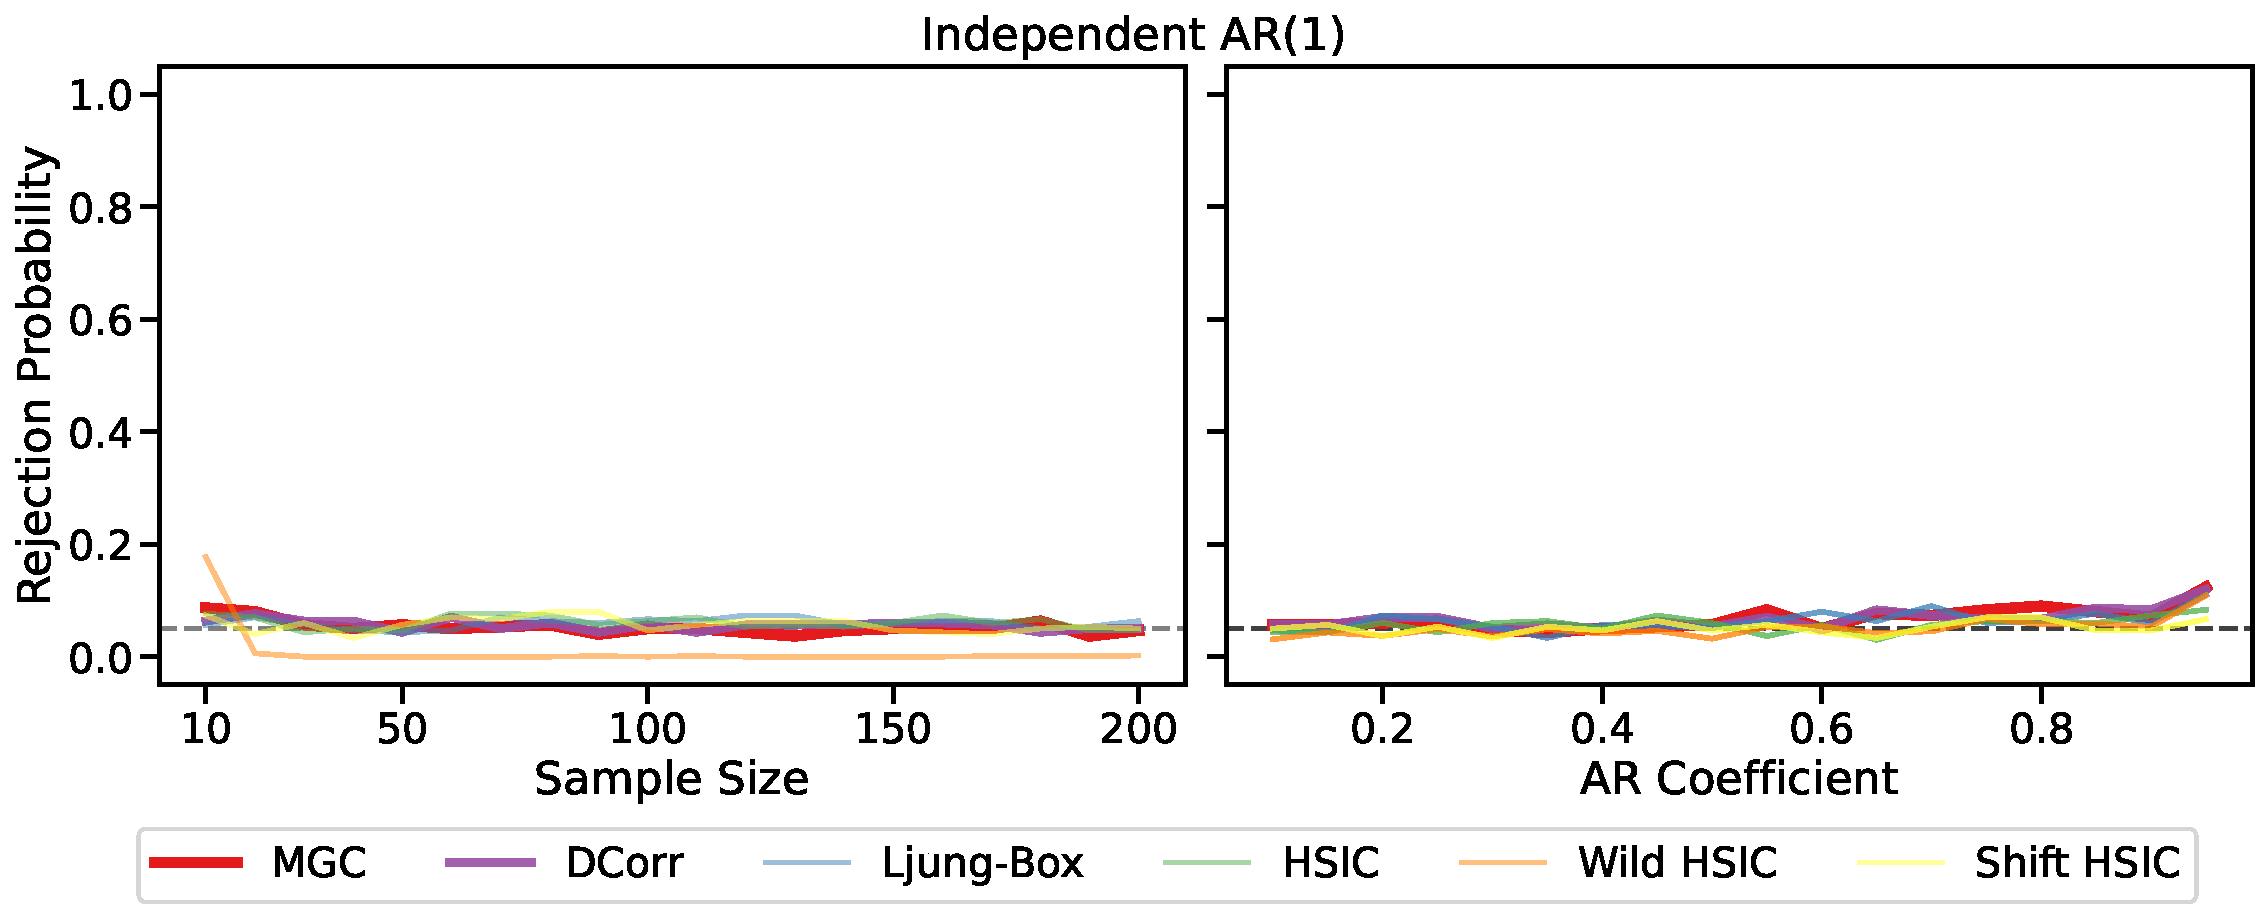
\includegraphics[width=0.9\textwidth]{figures/mgcx/figure1}
    \caption{This figure illustrates the validity of the tests using two independent time series. In the left panel, the testing power is computed as the sample size increases, with an AR coefficient of $\phi=0.5$. The right panel keeps the sample size at $n=1200$ while varying the AR coefficient $\phi$, with the noise variance appropriately adjusted by $(1 - \phi^2)$, based on the same simulation as in \cite{shifthsic}. The dashed black line represents the significance level $\alpha=0.05$. 
    } \label{fig:indep}
\end{figure}

\paragraph{Linear Dependence}
Next, we assess our methods' ability to capture linear relationships in the following simulation:
\begin{equation*}
    \begin{bmatrix}
    X_t\\
    Y_t
    \end{bmatrix}
    =
    \begin{bmatrix}
    0 & \phi\\
    \phi & 0
    \end{bmatrix}
    \begin{bmatrix}
    X_{t-1}\\
    Y_{t-1}
    \end{bmatrix}
    +
    \begin{bmatrix}
    \epsilon_t\\
    \eta_t
    \end{bmatrix}.
\end{equation*}
As this represents a straightforward linear relationship, the \texttt{\LB{}} test, based on auto-correlation, is expected to perform best. This is indeed the case in the left panel of Figure~\ref{fig:const}. Our proposed methods using $\dcorr${}, $\Mgc${}, and \hsic{} follow closely, quickly converging to perfect power around $n=100$. In contrast, the other competitors do not perform well in this scenario. This is not surprising, as the \shift~method is designed to detect whether $X_t$ and $Y_t$ are dependent at lag $0$, whereas the linear dependence here is of lag $1$. The \wild~method used a wild bootstrap method to estimate the null distribution, which can be inaccurate at small sample size.

\paragraph{Nonlinear Dependence}
The next simulation considers a nonlinear dependent model: 
\begin{equation*}
    \begin{bmatrix}
    X_t\\
    Y_t
    \end{bmatrix}
    =
    \begin{bmatrix}
    \epsilon_t Y_{t-1}\\
    \eta_t
    \end{bmatrix}.
\end{equation*}
In the right panel of Figure~\ref{fig:const}, our proposed methods utilizing $\dcorr${}, $\Mgc${}, and \hsic{} demonstrate superior performance compared to other competing methods. Notably, the \hsic{} and $\Mgc${} implementations exhibit better finite-sample power, as these two dependence measures are better at identifying nonlinear relationships than $\dcorr${}. In contrast, all other tests fail to detect dependence in this scenario. %It is worth noting that despite \wild~and \shift~performing poorly in the linear and nonlinear cases, their flaw comes from the test procedure and not the kernel dependence measure. Specifically,  when we use the kernel dependence measure in our proposed test, its performance aligns with that of the \dcorr~and$\Mgc$~implementations.

\begin{figure}[ht]
    \centering
    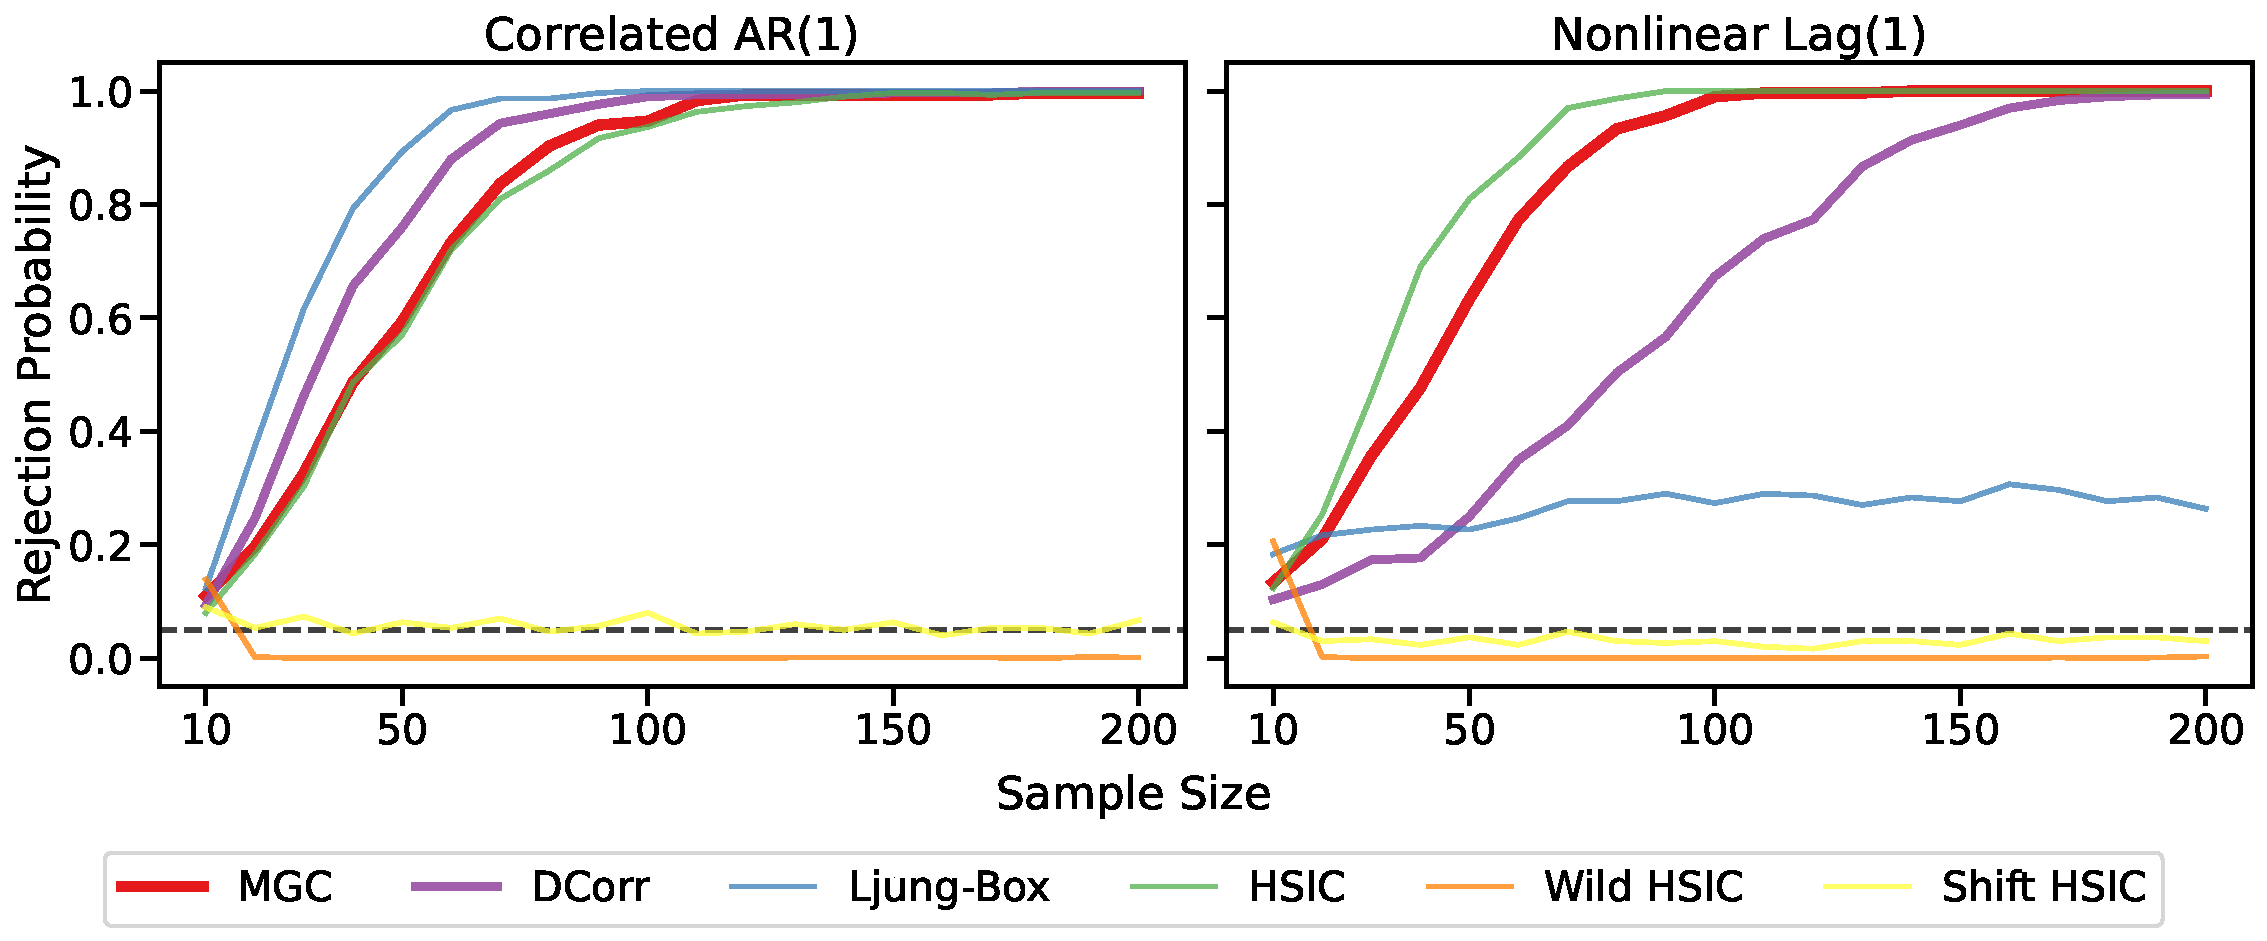
\includegraphics[width=0.9\textwidth]{figures/mgcx/figure2.pdf}
    \caption{The testing power for linear (left panel) and nonlinear (right panel) simulations based on $300$ replicates. } \label{fig:const}
\end{figure}

\paragraph{Extinct Gaussian} 
This simulation uses the same extinct Gaussian process from \cite{shifthsic}, where
\begin{equation*}
    \begin{bmatrix}
    X_t\\
    Y_t
    \end{bmatrix}
    =
    \begin{bmatrix}
    \phi & 0\\
    0 & \phi
    \end{bmatrix}
    \begin{bmatrix}
    X_{t-1}\\
    Y_{t-1}
    \end{bmatrix}
    +
    \begin{bmatrix}
    \epsilon_t\\
    \eta_t
    \end{bmatrix},
\end{equation*}
and we set $n=1200$. Here, the $(\epsilon_t, \eta_t)$ pair are dependent and drawn from an Extinct Gaussian distribution with two additional parameters: $e$ (extinction rate) and $r$ (radius). Both variables are initially drawn from independent standard normal, and $U$ is sampled from standard uniform. If either $\epsilon_t^2 + \eta_t^2 > r$ or $U > e$ holds, then $(\epsilon_t, \eta_t)$ are returned; otherwise, they are discarded and the process is repeated. In this process, the dependence between $\epsilon_t$ and $\eta_t$ increases with extinction rate $e$. Therefore, we expect power to increase with the extinction rate, which is indeed the case as shown in Figure \ref{fig:extinct}. While all methods, except \LB, are consistent and eventually achieve perfect power, our proposed method using $\Mgc${} stands out as the best performer.

\begin{figure}[ht]
    \centering
    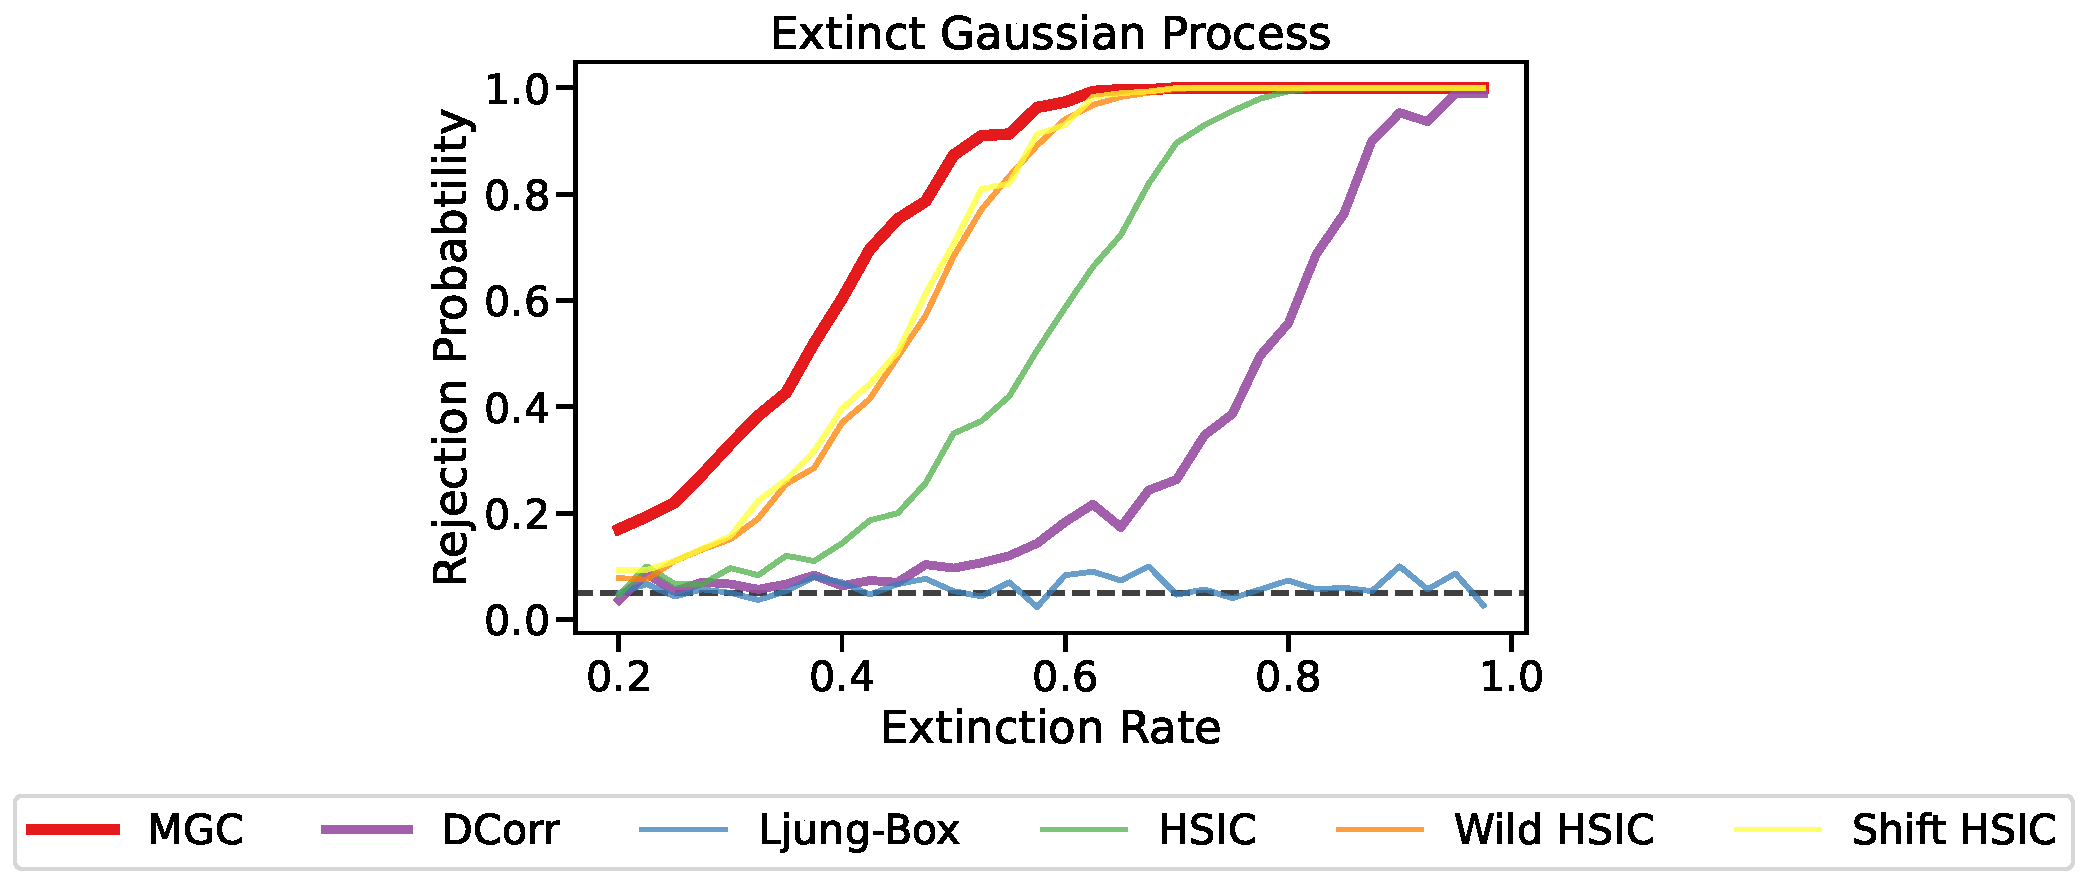
\includegraphics[width=1.0\textwidth]{figures/mgcx/figure3}
    \caption{The testing power for the extinct gaussian simulation based on $300$ replicates.} \label{fig:extinct}
\end{figure}

\subsection{Optimal Dependence Lag Estimation}
\label{sim2}
In this subsection, we evaluate the method's performance in estimating the optimal dependence lag in both linear and nonlinear settings. The linear setting is
\begin{equation*}
    \begin{bmatrix}
    X_t\\
    Y_t
    \end{bmatrix}
    =
    \begin{bmatrix}
    0 & \phi_1\\
    \phi_1 & 0
    \end{bmatrix}
    \begin{bmatrix}
    X_{t-1}\\
    Y_{t-1}
    \end{bmatrix}
    +
    \begin{bmatrix}
    0 & \phi_3\\
    \phi_3 & 0
    \end{bmatrix}
    \begin{bmatrix}
    X_{t-3}\\
    Y_{t-3}
    \end{bmatrix}
    +
    \begin{bmatrix}
    \epsilon_t\\
    \eta_t
    \end{bmatrix},
\end{equation*}
where we set $\phi_3=0.8  > \phi_1=0.1$ such that the true optimal dependence lag equals $3$.
The nonlinear simulation is
\begin{equation*}
    \begin{bmatrix}
    X_t\\
    Y_t
    \end{bmatrix}
    =
    \begin{bmatrix}
    \epsilon_t Y_{t-3}\\
    \eta_t
    \end{bmatrix}.
\end{equation*}
% 
In both simulations, the true optimal dependence lag equals $3$. Figure \ref{fig:lag} shows that the proposed method using either $\dcorr${} or $\Mgc${} consistently estimates the optimal dependence lag as the sample size increases, and $\Mgc$~outperforms $\dcorr$~in the nonlinear setting. 

\begin{figure}
    \centering
    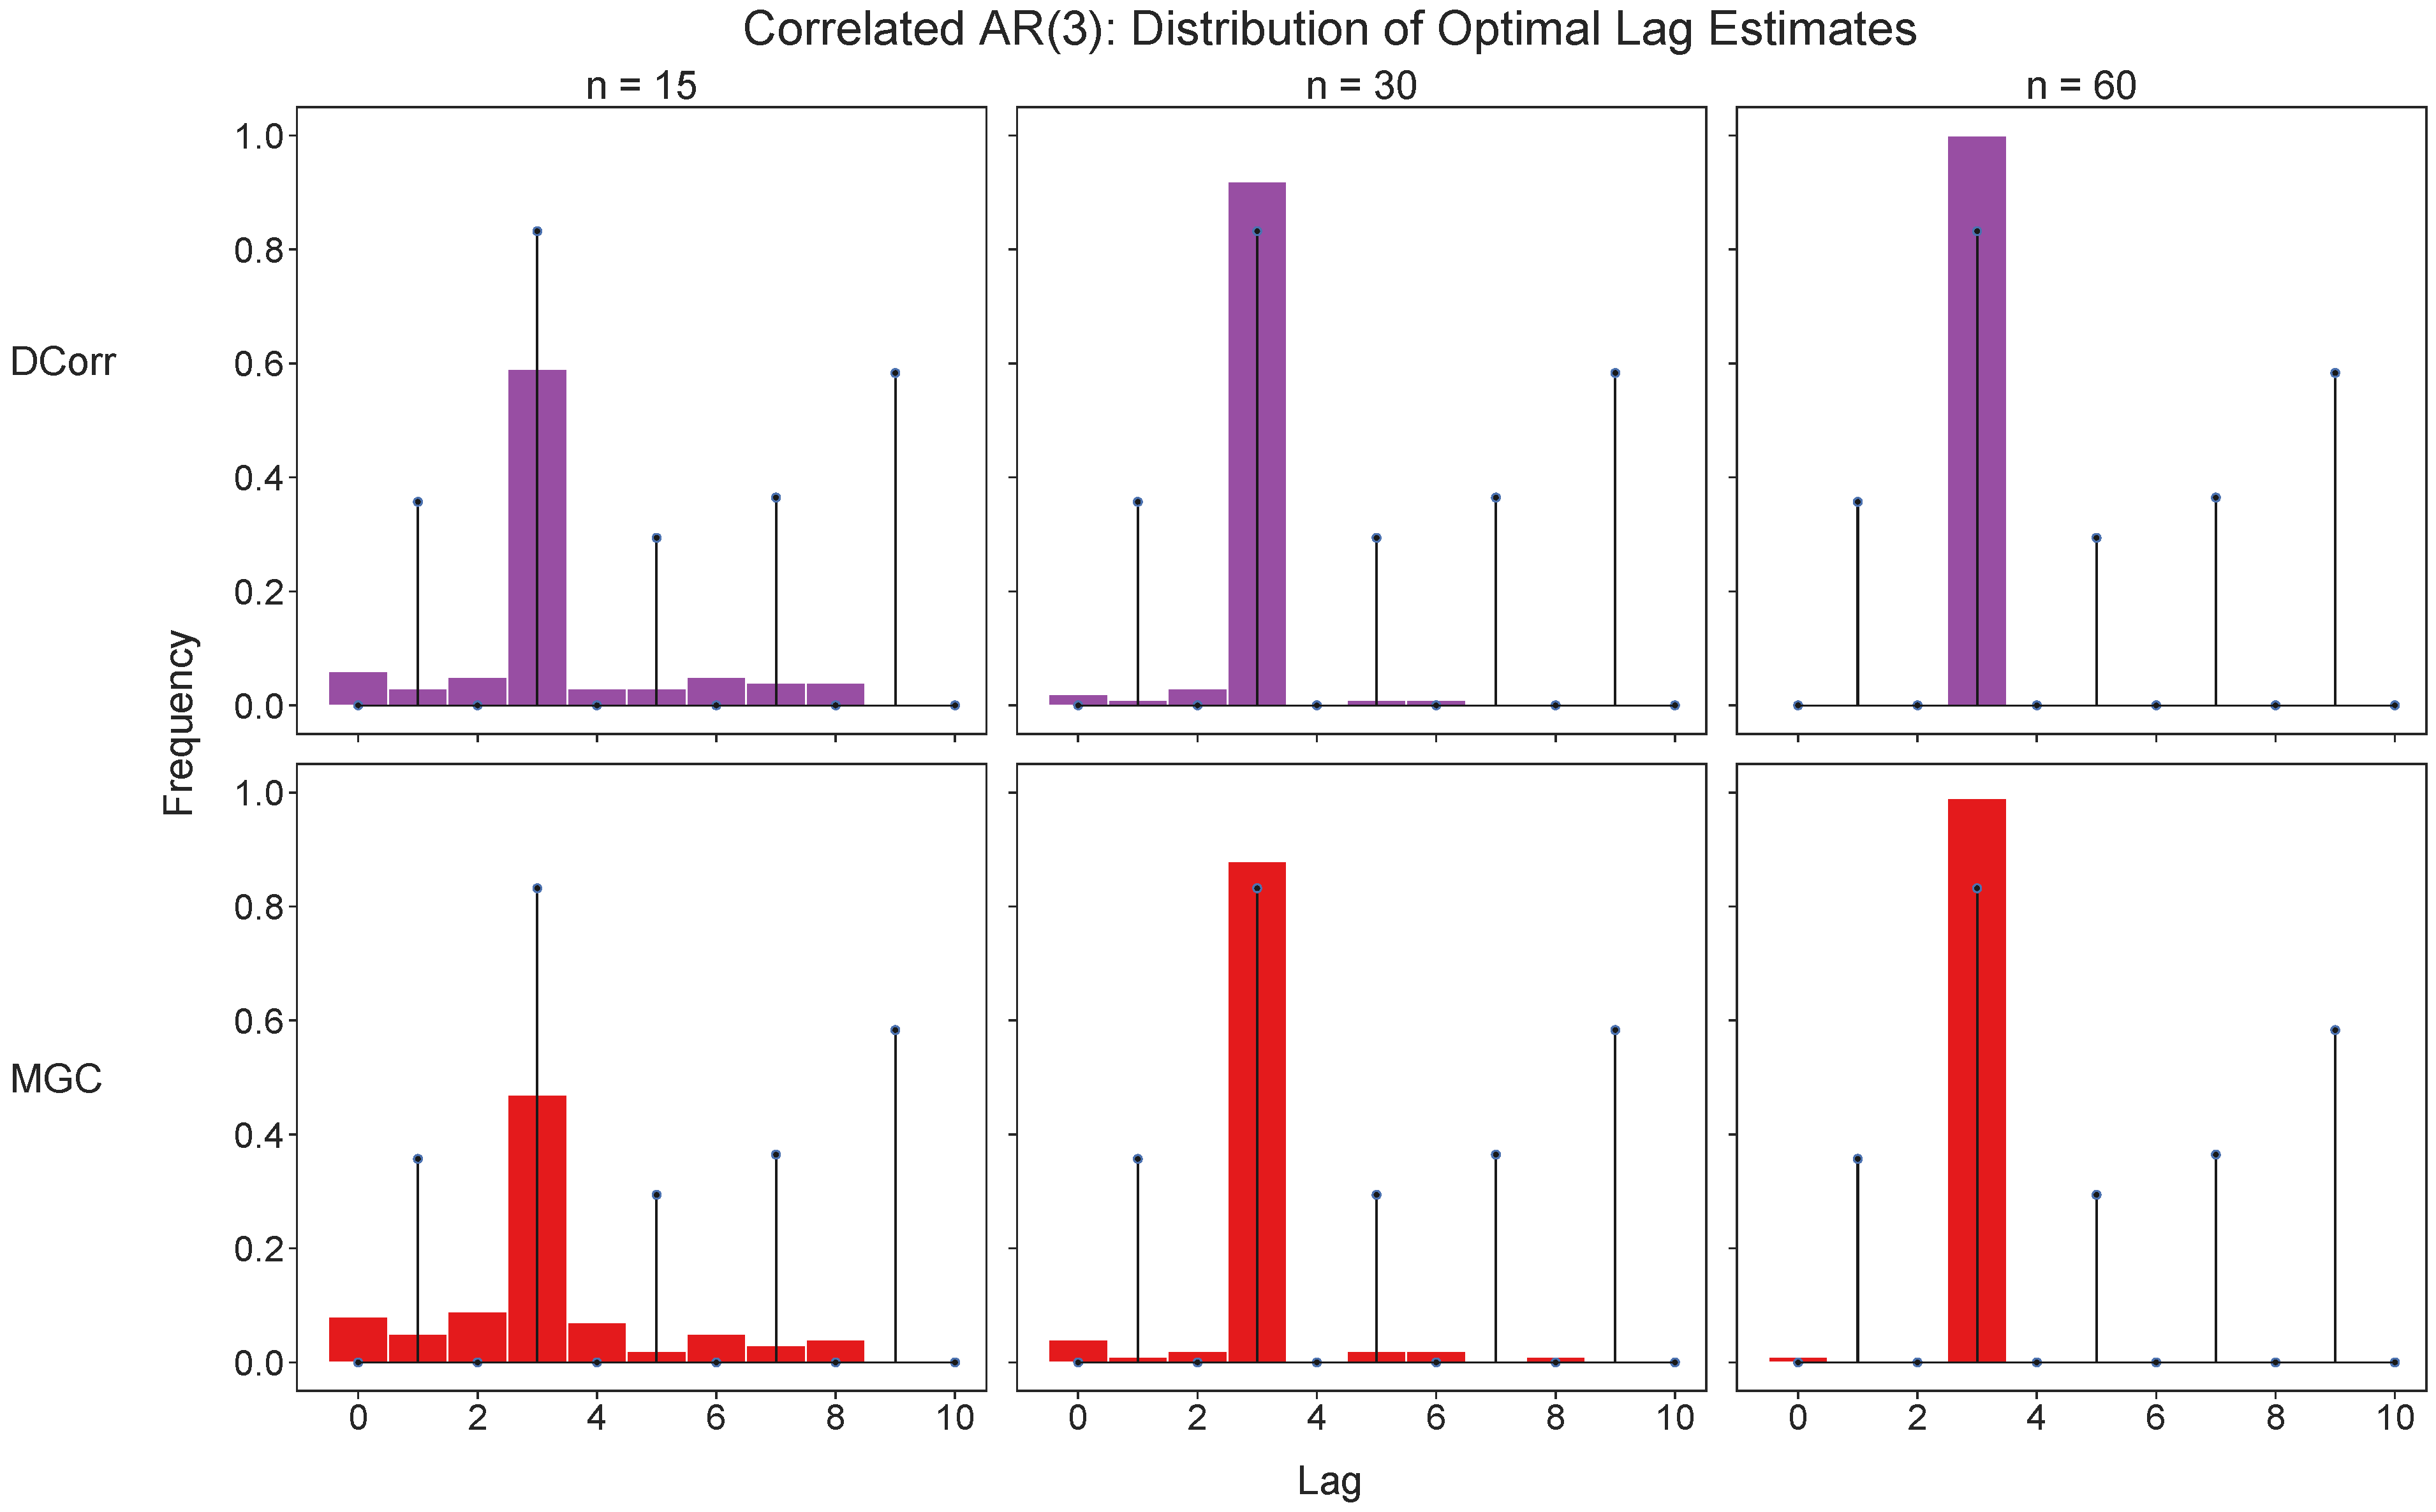
\includegraphics[width=0.9\textwidth]{figures/mgcx/opt_lag_sim_corr_ar3.pdf}
    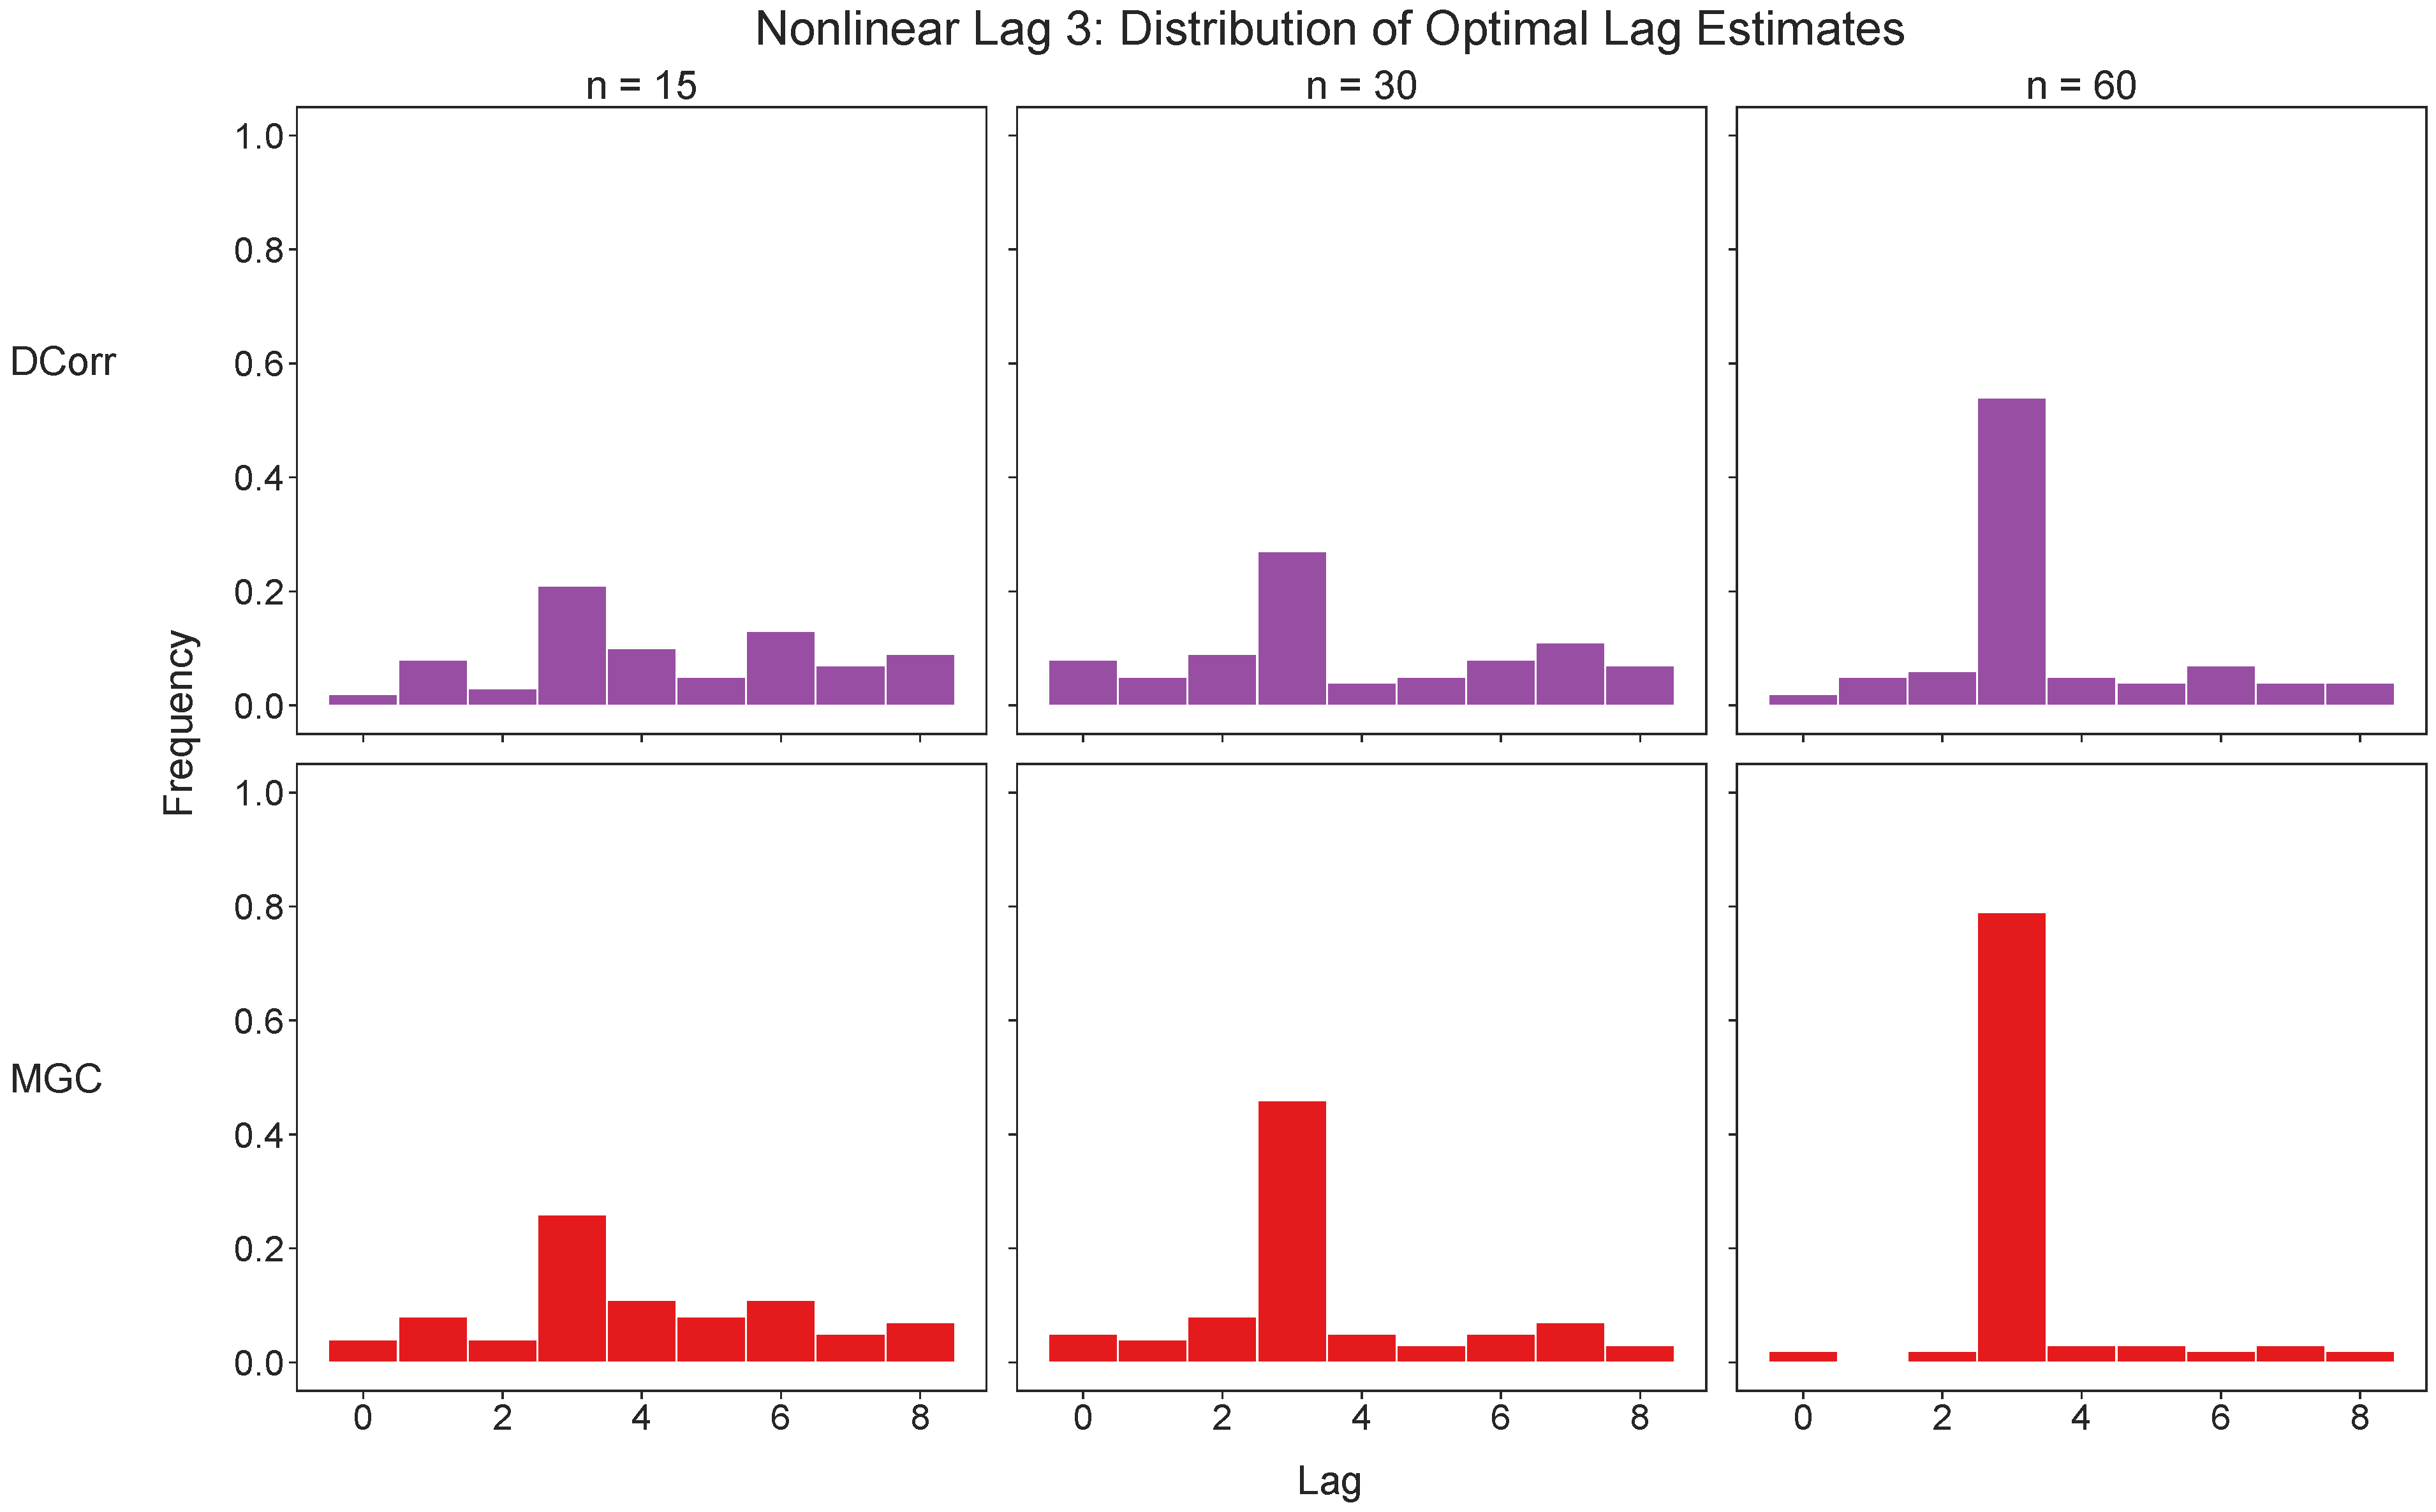
\includegraphics[width=0.9\textwidth]{figures/mgcx/opt_lag_sim_nonlin_lag3.pdf}
    \caption{This figure displays the performance of our proposed method using both $\Mgc$ and $\dcorr$ for estimating the optimal dependence lag $\hat{L}^{*}$ in linear and nonlinear relationships. The colored bar above lag $l$ shows the empirical frequency of $\hat{L}^{*}=j$, with red representing $\Mgc$ and purple representing $\dcorr$. The probability is estimated based on $100$ trials. The first row shows $\dcorr$ estimation performance at sample sizes $n=15, 30, 60$ for linear relationships, while the second row shows the $\Mgc$ performance on the same data. The third row displays $\dcorr$ estimation for nonlinear relationships, and the last row presents the same for $\Mgc$.
    } \label{fig:lag}
\end{figure}

\subsection{Multivariate Simulations}
In this subsection, we revisit the testing power and dependence lag estimation in both linear and nonlinear settings, maintaining a fixed sample size of $n=100$ and increasing the dimensionality $p$, to evaluate performance for multivariate data.

For testing power evaluation, we use the following multivariate linear setting:
\begin{equation*}
    \begin{bmatrix}
    X_t\\
    Y_t
    \end{bmatrix}
    =
    \begin{bmatrix}
    0 & \phi D\\
    \phi D & 0
    \end{bmatrix}
    \begin{bmatrix}
    X_{t-1}\\
    Y_{t-1}
    \end{bmatrix}
    +
    \begin{bmatrix}
    \epsilon_t\\
    \eta_t
    \end{bmatrix},
\end{equation*}
where $\phi = 0.65$, $D\in \mathbb{R}^{p\times p}$ is a diagonal matrix where the elements are $D_{ii} = 1 / i$, and $\epsilon_t, \eta_t$ are standard normal of dimension $p$. In a similar manner, we use the following multivariate nonlinear setting:
\begin{equation*}
    \begin{bmatrix}
    X_t\\
    Y_t
    \end{bmatrix}
    =
    \begin{bmatrix}
    D (\epsilon_t \odot Y_{t-1})\\ 
    \eta_t
    \end{bmatrix},
\end{equation*}
where $\odot$ denotes element-wise multiplication. We intentionally design the matrix $D$ as a decaying weight, reflecting a meaningful multivariate simulation where additional dimensions contain weaker dependence signals.

Figure~\ref{fig:multivariate1} illustrates the testing power as dimensionality increases. At a fixed sample size, all testing powers gradually decrease as $p$ increases. The proposed method using any of $\Mgc$, $\dcorr$, or \hsic~maintains relatively stable power with slow degradation in the case of linear dependence. The same trend is observed for nonlinear dependence, although the degradation is faster, with the $\Mgc$~statistic performing the best. It is worth emphasizing that due to the consistent property, if we fix $p$ and let $n$ increase, the testing power for our method shall increase to $1$. 

\begin{figure}
    \centering
    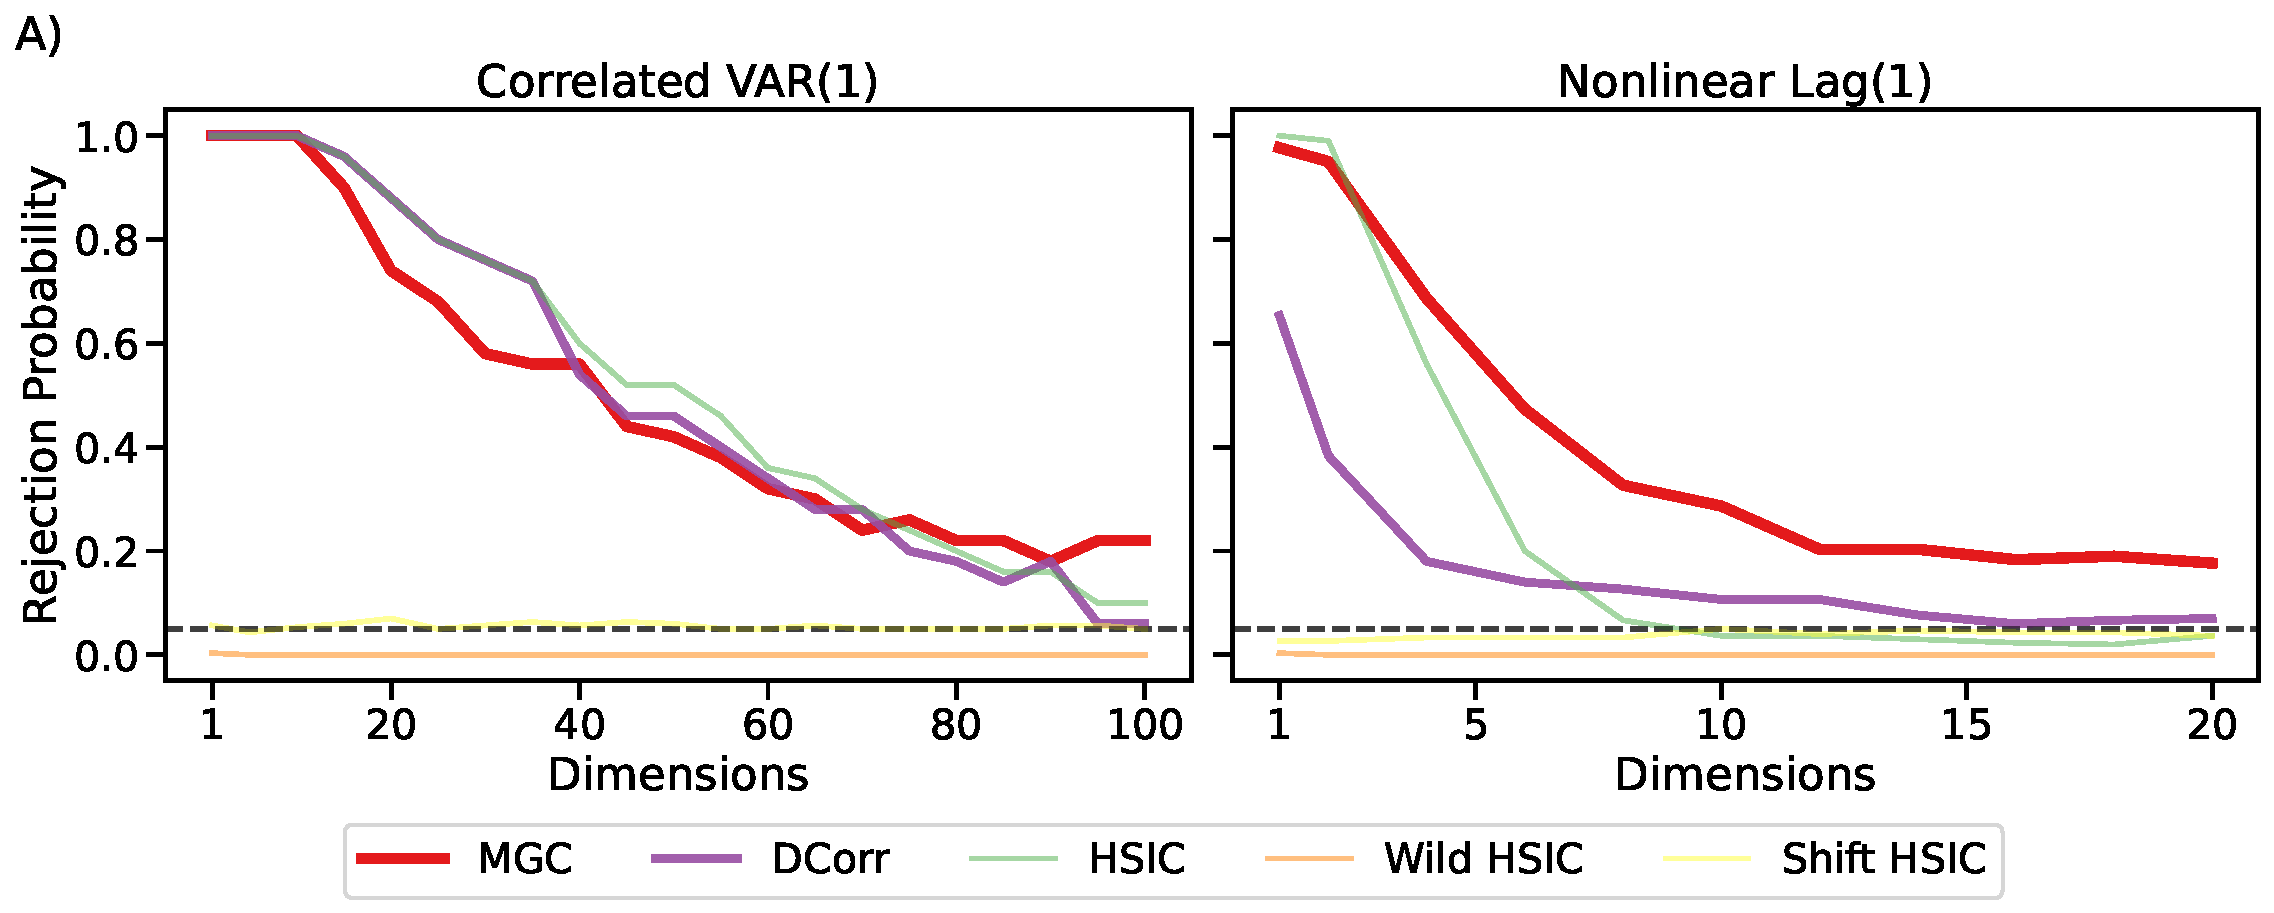
\includegraphics[width=0.9\textwidth]{figures/mgcx/multivariate_power.pdf}
    \caption{This figure shows the testing power for multivariate simulations, with a constant sample size of $n=100$ while increasing the dimensionality.
    } \label{fig:multivariate1}
\end{figure}

Similarly, we extend the optimal lag estimation into the following two multivariate settings: 
\begin{align*}
    \begin{bmatrix}
    X_t\\
    Y_t
    \end{bmatrix}
    &=
    \begin{bmatrix}
    0 & \phi_1 D\\
    \phi_1 D & 0
    \end{bmatrix}
    \begin{bmatrix}
    X_{t-1}\\
    Y_{t-1}
    \end{bmatrix}
    + 
    \begin{bmatrix}
    0 & \phi_3 D\\
    \phi_3 D & 0
    \end{bmatrix}
    \begin{bmatrix}
    X_{t-3}\\
    Y_{t-3}
    \end{bmatrix}
    +
    \begin{bmatrix}
    \epsilon_t\\
    \eta_t
    \end{bmatrix}.\\
    \begin{bmatrix}
    X_t\\
    Y_t
    \end{bmatrix}
    &=
    \begin{bmatrix}
    D (\epsilon_t \odot Y_{t-3})\\
    \eta_t
    \end{bmatrix},
\end{align*}
where $\phi_1 = 0.1$ and $\phi_3= 0.65$. These settings are similar to those in Section~\ref{sim2}, with the addition of increasing dimension and $D$. The true optimal lag remains $3$. The estimation accuracy, as shown in Figure~\ref{fig:multivariate2}, demonstrates successful detection at small $p$, with accuracy gradually degrading as $p$ increases.

\begin{figure}
    \centering
    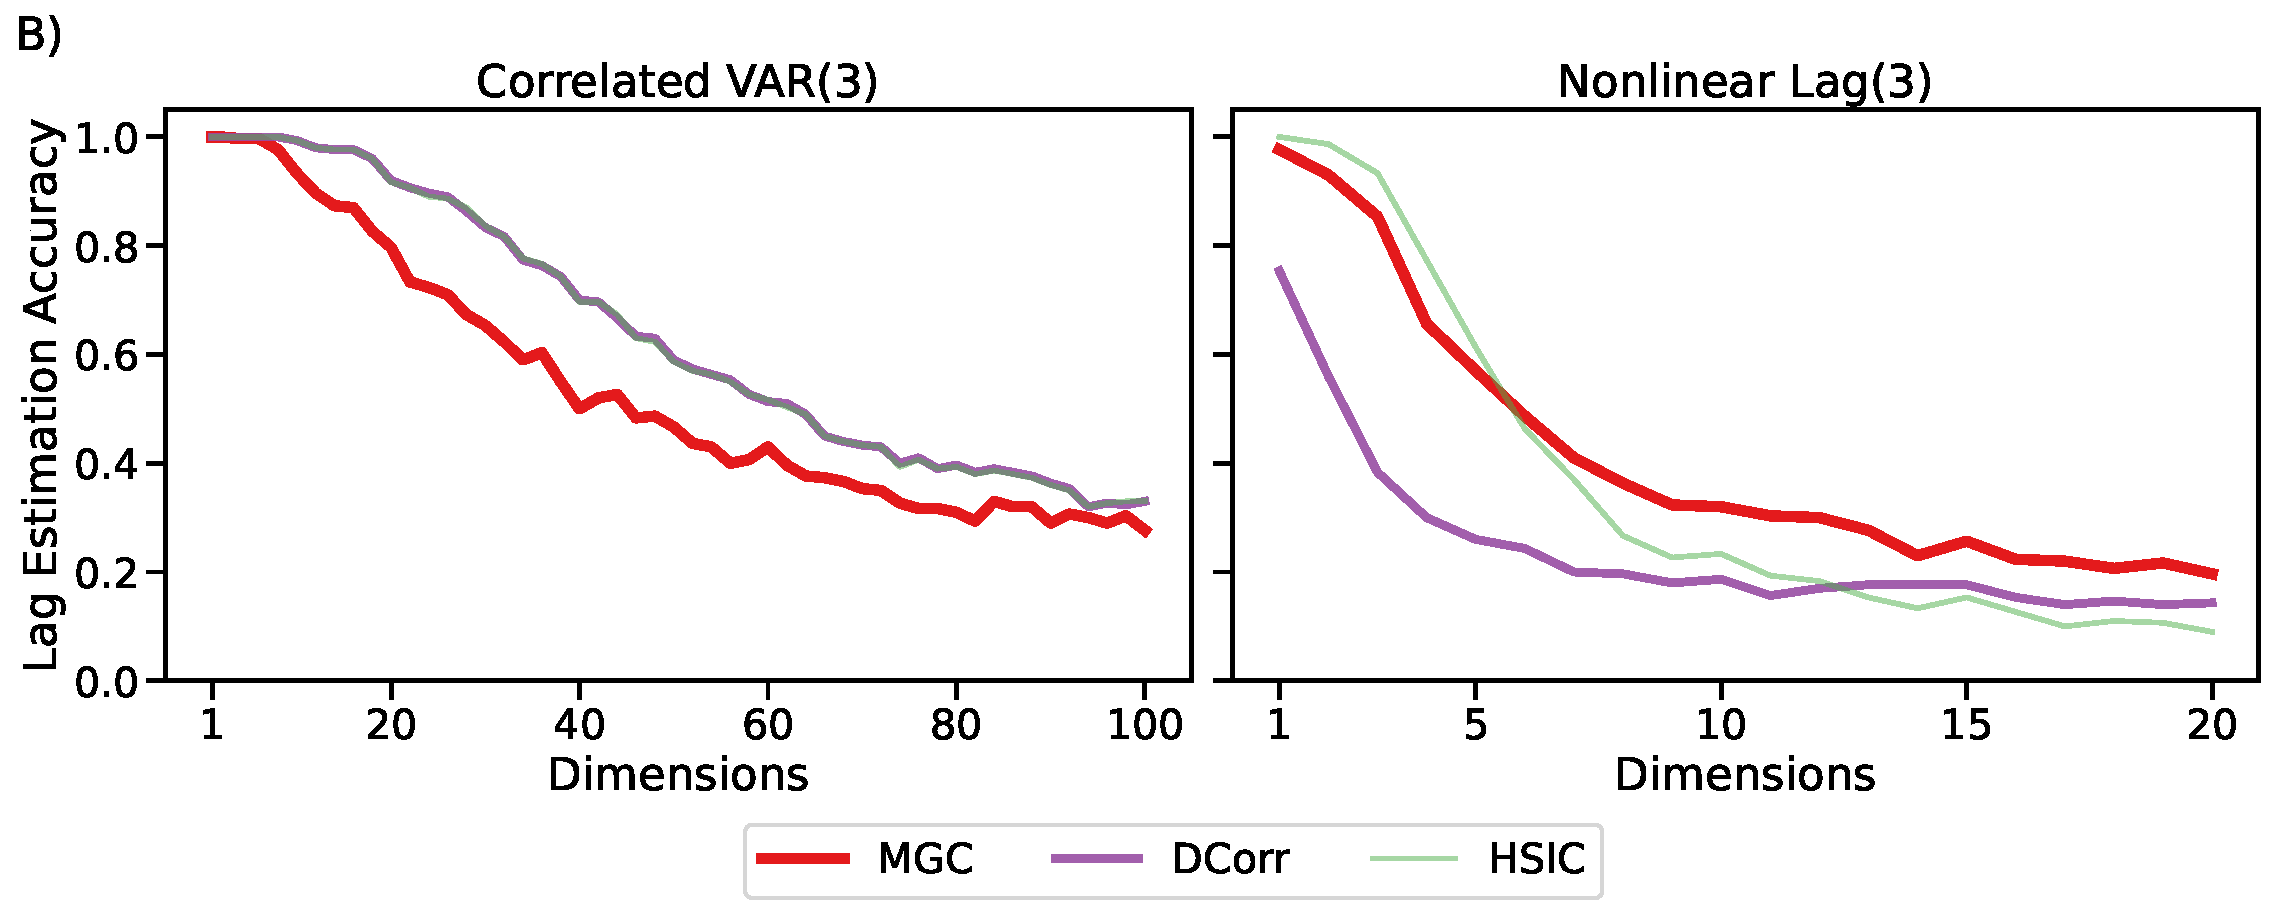
\includegraphics[width=0.9\textwidth]{figures/mgcx/multivariate_lag.pdf}
    \caption{This figure shows the accuracy of estimating the true optimal lag in multivariate simulations, maintaining a constant sample size of $n=100$ while increasing the dimensionality. Note that in the left panel, the lines representing $\dcorr$~ and \hsic~ overlap due to their almost identical performance.
    } \label{fig:multivariate2}
\end{figure}

\section{Analyzing Connectivity in the Human Brain}
\label{sec:app}

This study is based on data from an individual (Subject ID: 100307) of the Human Connectome Project (HCP), which can be downloaded online\footnote{\url{https://www.humanconnectome.org/study/hcp-young-adult/data-releases}}. The human cortex is parcellated into 180 parcels per hemisphere using the HCP multi-modal parcellation atlas \cite{glasser}. For this study, 22 parcels were selected as regions of interest (ROIs), representing various locations across the cortex. These parcels are denoted as $X^{(1)}, \dots, X^{(22)}$. Each parcel consists of a contiguous set of vertices whose fMRI signal is projected on the cortical surface. Averaging the vertices within a parcel yields a univariate time series $X^{(u)} = (X^{(u)}_1, \dots, X^{(u)}_n)$, where $n = 1200$ in this particular case.
The selected ROIs, their parcel number in the HCP multi-modal parcellation \cite{glasser}, and assigned network are listed in Table \ref{fig:roi}. 
\begin{table}[ht]
    \centering
    \begin{tabular}{ l | l | l | l | l}
     ROI ID & Network & Shorthand & Parcel Key & Parcel Name\\ 
     \hline
     1 & Visual Network & Visual & 1 & V1\\
     2 & Visual Network & Visual	& 23 & MT\\
     3 & Visual Network & Visual	& 18 & FFC\\
     4 & Somatomotor Network & SM	& 53 & 3a\\
     5 & Somatomotor Network & SM	& 24 & A1\\
     6 & Dorsal Attention Network & dAtt & 96 & 6a\\
     7 & Dorsal Attention Network & dAtt & 117 & API\\
     8 & Dorsal Attention Network & dAtt & 50 & MIP\\
     9 & Dorsal Attention Network & dAtt & 143 & PGp\\
     10 & Ventral Attention Network & vAtt & 109 & MI\\
     11 & Ventral Attention Network & vAtt & 148 & PF\\
     12 & Ventral Attention Network & vAtt & 60 & p32pr\\
     13 & Ventral Attention Network & vAtt & 38 & 23c\\
     14 & Limbic Network & Limbic & 135 & TF\\
     15 & Limbic Network & Limbic & 93 & OFC\\
     16 & FrontoParietal Network & FP & 83 & p9-46v\\
     17 & FrontoParietal Network & FP & 149 & PFm\\
     18 & Default Mode Network & DMN & 150 & PGi\\
     19 & Default Mode Network & DMN & 65 & p32pr\\
     20 & Default Mode Network & DMN & 161 & 32pd\\
     21 & Default Mode Network & DMN & 132 & TE1a\\
     22 & Default Mode Network & DMN & 71 & 9p
    \end{tabular}
    \caption{This table displays the parcellation information for the parcels used in our analysis. The first column shows the numeric order of the parcels as they appear in the following figures. The second and third columns show the shorthand and full names, respectively, of the network to which each parcel belongs. The last two columns display the parcel number and name according to the \cite{glasser} parcellation.}
    \label{fig:roi}
\end{table}

As the temporal dependence method using $\Mgc$~performed well in our simulations, we simply use the $\Mgc$~implementation in this analysis. In the left panel of Figure \ref{fig:app}, we present the optimal dependence lag for each interdependency, ranging up to $L=10$. Meanwhile, the right panel of Figure \ref{fig:app} displays the log-scale $p$-values of temporal dependence for each pair of parcels. Generally, we observe strong relationships with small lags within the same region, such as an optimal lag of usually $0$ within the "DMN" region with significant p-values. In contrast, inter-region dependencies are less significant and typically exist at longer lags.
% 

\begin{figure}
    \centering
    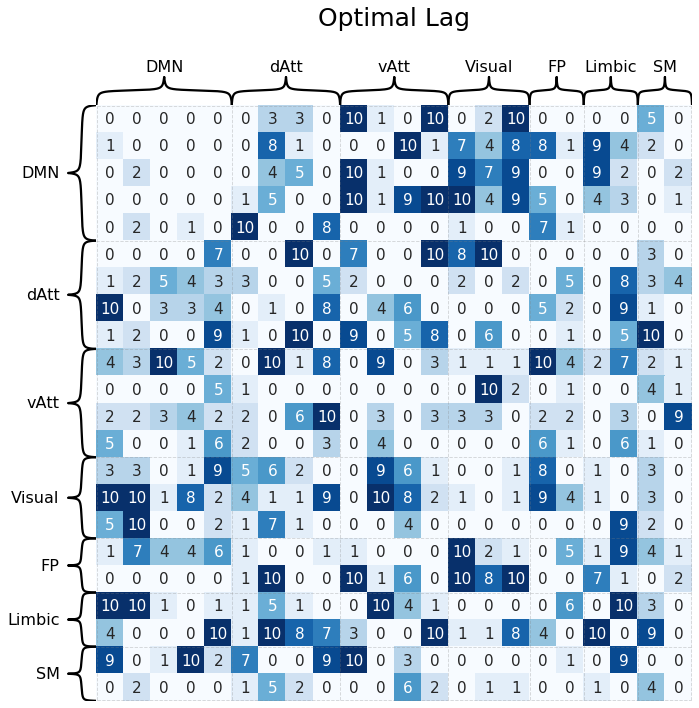
\includegraphics[width=0.42\linewidth]{figures/mgcx/optimal_lag.png}
    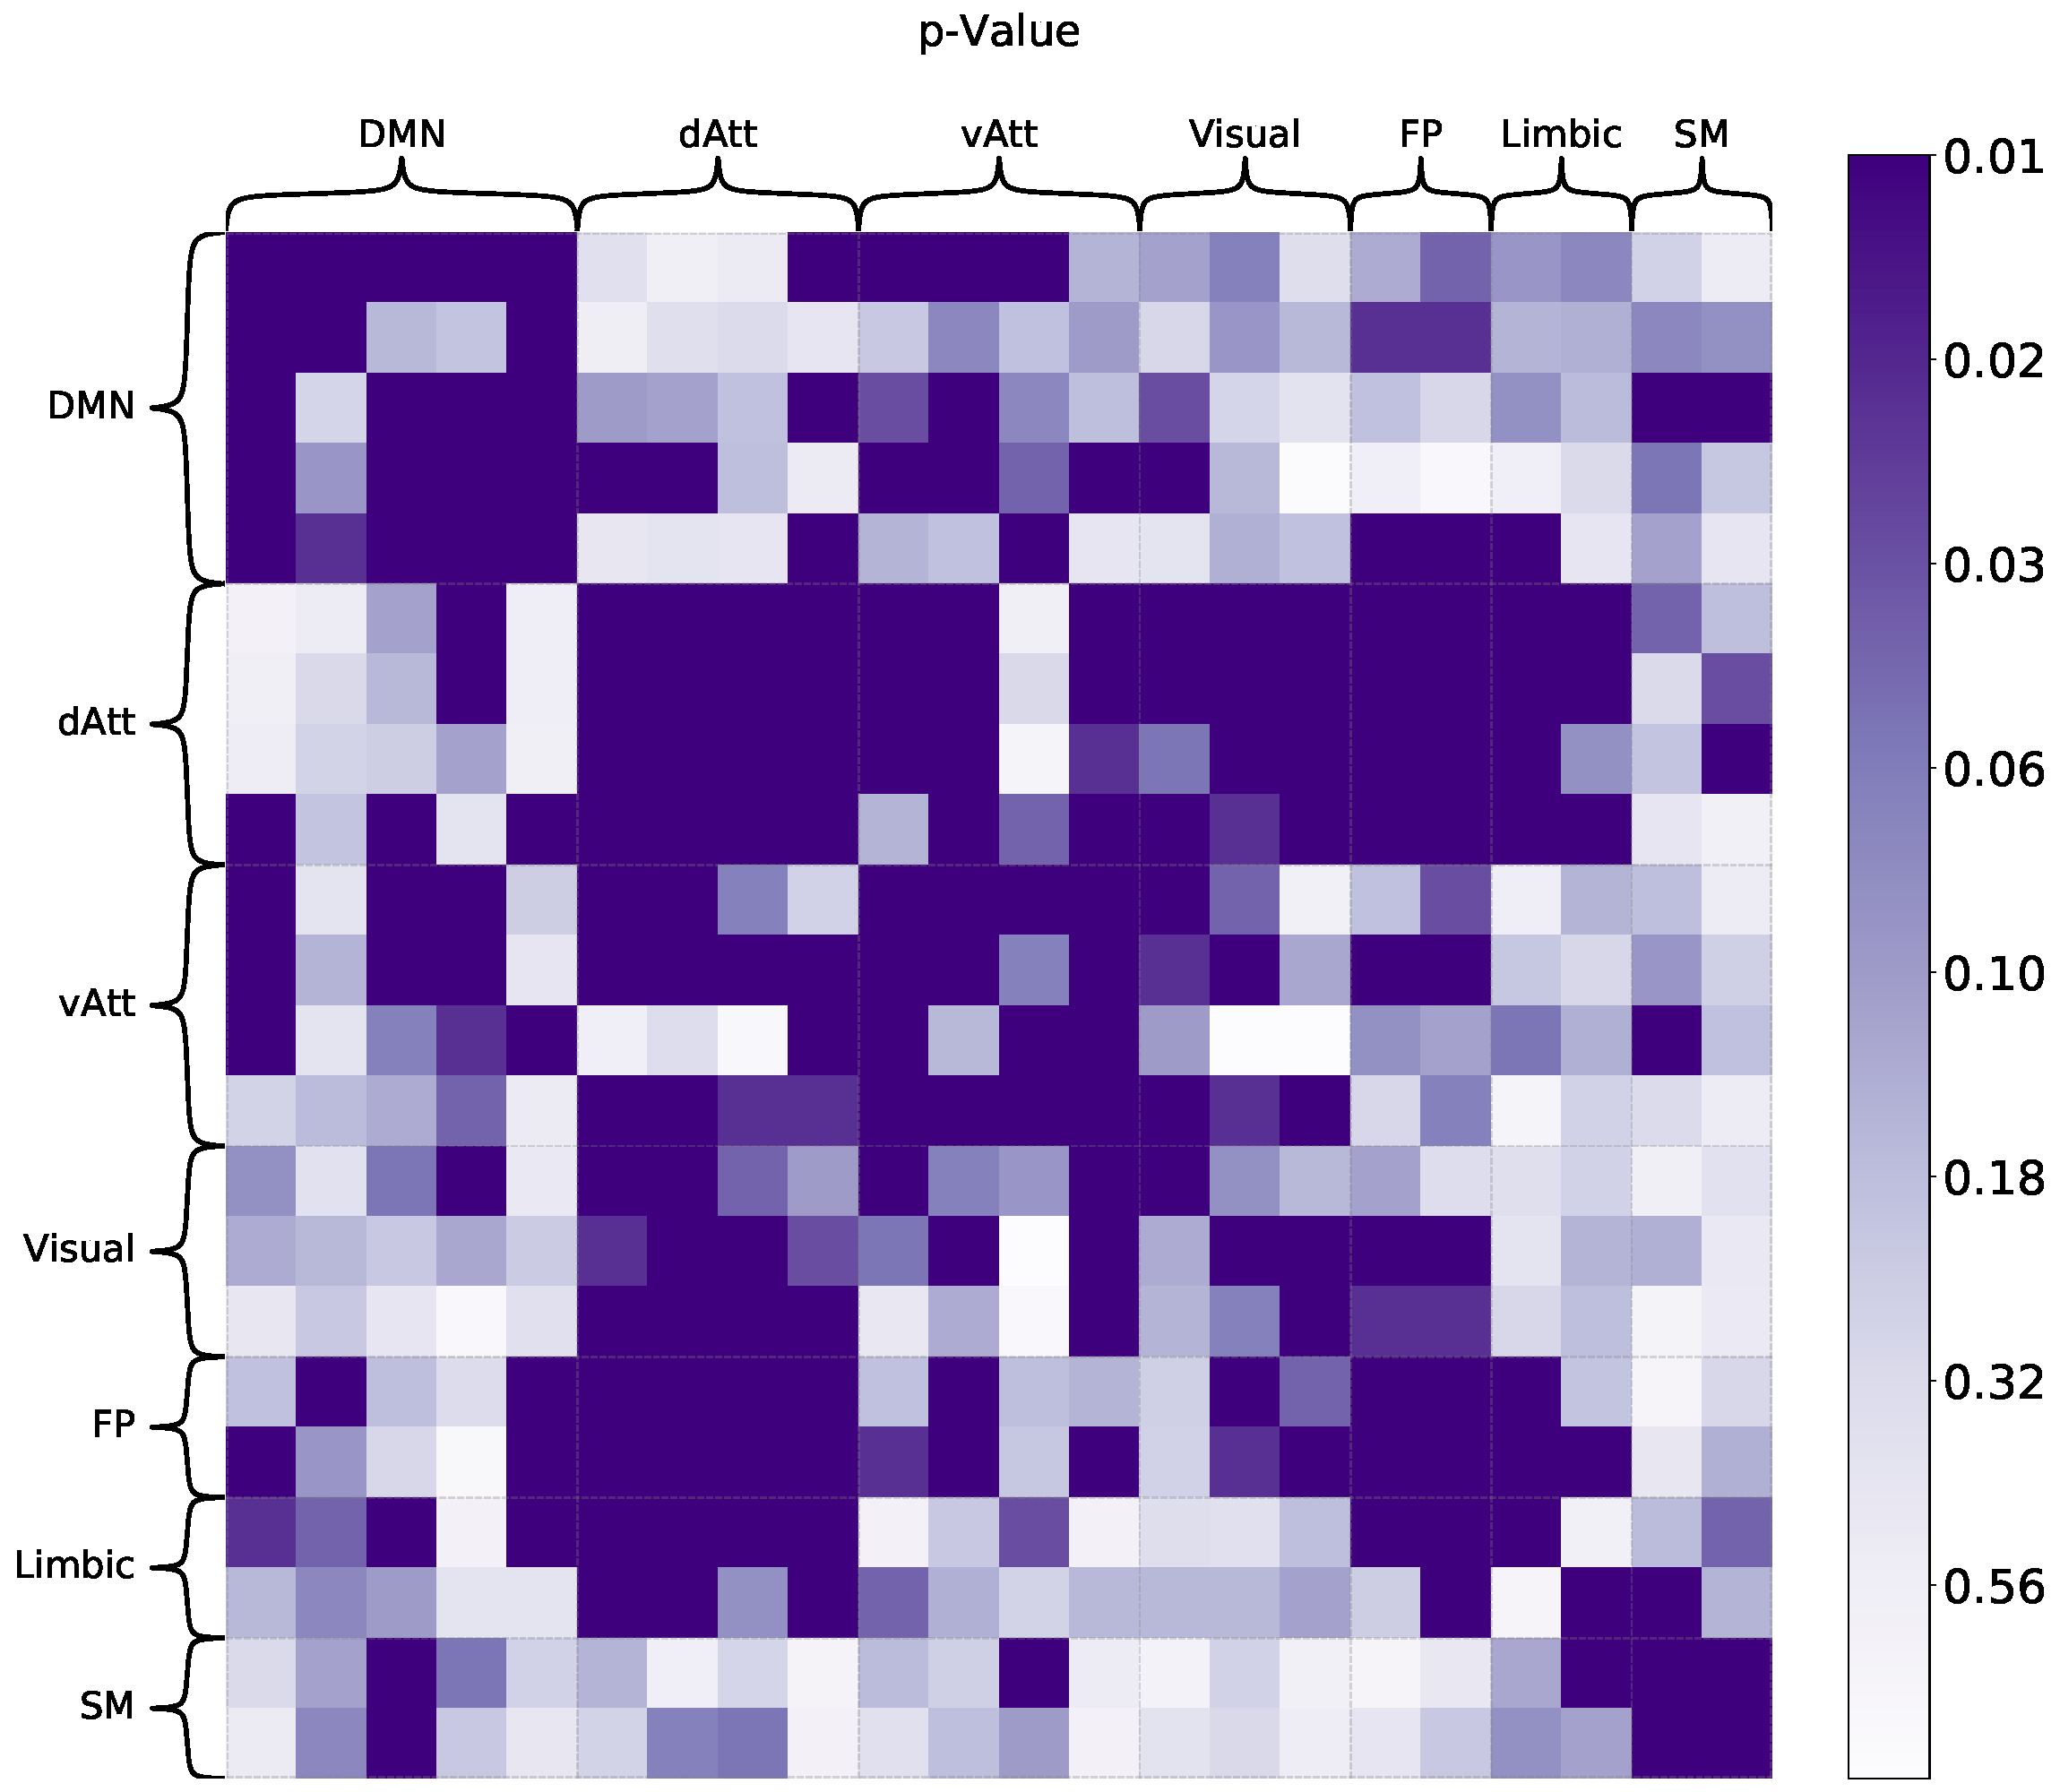
\includegraphics[width=0.48\linewidth]{figures/mgcx/pval.pdf}
    %\includegraphics[width=0.95\linewidth]{optimal_scale.png}
    \caption{This displays the results of applying the temporal dependence method using $\Mgc$ to resting-state fMRI data. 
    }
    \label{fig:app}
\end{figure}

%n addition, Figure \ref{fig:app} (bottom) presents the optimal scale at which the local correlation is maximized. 
%for pairs of time series ${X^{(u)}_t}$ and ${X^{(v)}_t}$. 
%Many of the time series pairs within the default mode and visual networks exhibit a normalized optimal scale of (1,1), suggesting a linear dependence between the signals in these regions. In contrast, nonlinear dependencies are observed among pairs of signals in many other networks.


\section{Conclusion}
\label{sec:discussion}
This paper introduces a new independence testing procedure for temporal data. The method combined the strengths of nonparametric dependence measures, the specialized cross-lag statistic for time series, and the block permutation procedure. As a result, it provides an asymptotically valid and universally consistent approach with outstanding numerical performance. While the exposition of this manuscript is focused on time series data, this work marks an important step in extending independence testing to structural data beyond the realm of standard i.i.d.~data, making them more attractive and broadly applicable.

There are several avenues for future research that warrant exploration. Firstly, although we have demonstrated the asymptotic validity of the block permutation test, its computational efficiency remains a challenge when dealing with large sample sizes. Recent studies \cite{zhang2018,fast1} have investigated faster testing procedures by approximating the null distribution of distance and kernel correlations under the standard i.i.d.~setting. Extending such approaches to structural data could significantly enhance computational scalability.

Secondly, dependence measures are commonly employed in dimension reduction techniques, such as screening \cite{FanLv2008,LiZhongZhu2012}, especially in high-dimensional data settings. However, little attention has been given to the temporal domain. While it is straightforward to utilize dependence measures for dimension reduction in multivariate time series, delving into their theoretical properties and their relationships with other standard tools, such as independence component analysis, could provide valuable insights.

Thirdly, causal inference in time series data is an important task \cite{haufe2010sparse,winkler2016validity}. While it is widely recognized that correlation does not imply causality, recent research has demonstrated the utility of dependence and conditional dependence tests in causal inference \cite{cai2022distribution,laumann2023kernel}. Therefore, extending this framework to encompass conditional independence and causal inference may significantly advance the understanding of causal inference in time series data.

\section{Supplemental Materials}
\subsection{Assumptions}
We begin by revisiting the theoretical assumptions listed in the main paper:
\begin{itemize}
\item The observed data $\{(X_t, Y_t)\}_{t=1}^{n}$ is strictly stationary, non-constant, and the underlying distribution $F_{XY_{-l}}$ has finite moments for any lag $l \geq 0$. 
\item There exists a maximum dependence lag $M$ such that for all $l \geq M$, the two time series are almost independent for large $n$, so are each time series within itself:
    \begin{align*}
        \sup|F_{X Y_{-l}} - F_{X}F_{Y}| &= O(\frac{1}{n}) ,\\
        \sup|F_{X X_{-l}} - F_{X}F_{X}| &= O(\frac{1}{n}) ,\\
        \sup|F_{Y Y_{-l}} - F_{Y}F_{Y}| &= O(\frac{1}{n}) .
    \end{align*}
\item The maximum dependence lag $M$ and the maximum lag under consideration $L$ are non-negative integers that satisfies $L \geq M$ and $L=o(n)$, i.e., they may increase together with $n$ but at a slower pace.
\item As the sample size $n$ increases, both the number of blocks $B$ and the number of observations per block $\frac{n}{B}$ increase to infinity. Moreover, $\frac{n}{B} \geq M$ for sufficiently large $n$.
\item The sample dependence measure has the following form:
\begin{align*}
        \TDCor_{n}(\vec{X},\vec{Y}) &=\frac{\sum_{i=1}^{n}\sum_{j=1}^{n} \gamma_{n}(i,j)}{n^2},
    \end{align*} 
    where each $\gamma_{n}(i,j)$ is a function of $(X_i,X_j, Y_i,Y_j)$, and remaining sample pairs may also be used but with a weight of $O(1/n)$.
\item In the standard i.i.d.~setting where $(X_1,Y_1), (X_2, Y_2),\ldots, (X_n, Y_n) \stackrel{i.i.d.}{\sim} F_{XY}$, there exists a population statistic $\TDCor(X, Y)$ defined solely based on the joint distribution $F_{XY}$. Each term in the sample statistic satisfies:
\begin{align*}
        \EE(\gamma_{n}(i,j)) &= \TDCor(X, Y) + o(1).
    \end{align*} 
    Moreover, the population statistic $\TDCor(X, Y)$ is non-negative and equals $0$ if and only if $X$ and $Y$ are independent, i.e., $F_{XY}=F_{X} F_{Y}$.
\end{itemize}

\subsection{Theorem Proofs}
\begin{theorem}
     The cross dependence sample statistic satisfies:
    \begin{align*}
     \\EE(\TDCor_{n}(\vec{X}, \vec{Y}_{-l})) - \TDCor(X, Y_{-l}) = o(1),\\
     \text{Var}(\TDCor_{n}(\vec{X}, \vec{Y}_{-l}))  = O(\frac{1}{n-l}).
     \end{align*}

     Therefore, for each $l \in \{0,...,L\}$, we have
     \begin{align*}
     \TDCor_{n}(\vec{X}, \vec{Y}_{-l}) \stackrel{n \rightarrow \infty}{\rightarrow} \TDCor(X, Y_{-l})
     \end{align*}
     in probability.
\end{theorem}
\begin{proof}
First, applying the assumptions on the dependence measure to the cross dependence statistics yields:
\begin{align*}
\TDCor_{n}(\vec{X}, \vec{Y}_{-l}) &=\frac{\sum_{i=l+1}^{n}\sum_{j=l+1}^{n} \gamma_{n-l}(i,j)}{(n-l)^2}, \\
\EE(\gamma_{n-l}(i,j)) &= \TDCor(X, Y_{-l}) + o(1).
\end{align*}
Here, each $\gamma_{n-l}(i,j)$ is a function of $(X_i,X_j, Y_{i-l},Y_{j-l})$, and remaining sample pairs like $(X_u,X_v, Y_{w},Y_{z})$ may also be used but with a weight of $O(1/n)$.

As expectations are additive, it immediately follows that 
\begin{align*}
\EE(\TDCor_{n}(\vec{X}, \vec{Y}_{-l})) &= \frac{\sum_{i=l+1}^{n}\sum_{j=l+1}^{n} \EE(\gamma_{n-l}(i,j))}{(n-l)^2}\\
&= \frac{\sum_{i=l+1}^{n}\sum_{j=l+1}^{n} \{\TDCor(X, Y_{-l}) + o(1)\}}{(n-l)^2} \\
&= \TDCor(X, Y_{-l}) + o(1).
\end{align*}
Next, the variance equals
\begin{align*}
\text{Var}(\TDCor_{n}(\vec{X}, \vec{Y}_{-l})) &= \frac{Cov(\sum_{i=l+1}^{n}\sum_{j=l+1}^{n} \gamma_{n-l}(i,j), \sum_{u=l+1}^{n}\sum_{v=l+1}^{n} \gamma_{n-l}(u,v))}{(n-l)^4}.
\end{align*}
Therefore, it suffices to consider each covariance term $Cov(\gamma_{n-l}(i,j),\gamma_{n-l}(u,v))$, and there are $(n-l)^4$ such terms. 

When both $|u-i|>M$ and $|v-j|>M$, the maximum dependent lag possible, we have
\begin{align*}
Cov(\gamma_{n-l}(i,j),\gamma_{n-l}(u,v)) =  O(\frac{1}{n-l}).
\end{align*}
Otherwise it is
\begin{align*}
Cov(\gamma_{n-l}(i,j),\gamma_{n-l}(u,v))=  O(1).
\end{align*}
There are a total of $O((n-l)^2(n-M)^2)$ covariance terms of magnitude $O(\frac{1}{n-l})$, while the remaining $O((n-l)^3)$ covariance terms are of magnitude $O(1)$. Consequently, as $M=o(n)$, we have
\begin{align*}
\text{Var}(\TDCor_{n}(\vec{X}, \vec{Y}_{-l})) &= \frac{O((n-l)^2(n-M)^2) * O(\frac{1}{n-l}) + O((n-l)^3) * O(1)}{(n-l)^4}\\
&= O(\frac{1}{n-l}),
\end{align*}
which converges to $0$ as $n$ increases.

With the expectation converging to the population statistic and the variance approaching $0$, we can conclude that
\begin{align*}
     \TDCor_{n}(\vec{X}, \vec{Y}_{-l}) \stackrel{n \rightarrow \infty}{\rightarrow} \TDCor(X, Y_{-l})
     \end{align*}
     in probability.
\end{proof}

\begin{theorem}
    The temporal dependence sample statistic satisfies:
    \begin{align*}
     \TDCorX_{n}(\vec{X}, \vec{Y}) \stackrel{n \rightarrow \infty}{\rightarrow} \sum_{l=0}^{L}\TDCor(X, Y_{-l}).
     \end{align*}
     The estimated optimal dependence lag satisfies:
     \begin{align*}
     \hat{L}^{*} \stackrel{n \rightarrow \infty}{\rightarrow} \arg\max_{l \in [0,L]} \TDCor(X, Y_{-l}).
     \end{align*}
\end{theorem}
\begin{proof}
By Theorem~\ref{thm:sampling_dist}, each $\TDCor_{n}(\vec{X}, \vec{Y}_{-l})$ converges to $\TDCor(X, Y_{-l})$ with a variance of $O(\frac{1}{n-l})$.

Recall the definition of the temporal dependence statistic $\TDCorX_{n}(\vec{X}, \vec{Y})$ as
\begin{align*}
\TDCorX_{n}(\vec{X}, \vec{Y}) &= \sum_{l=0}^{L} \left(\frac{n-l}{n}\right) \cdot \TDCor_{n}(\vec{X}, \vec{Y}_{-l}).
\end{align*}
Then the expectation satisfies
\begin{align*}
\EE(\TDCorX_{n}(\vec{X}, \vec{Y})) &= \sum_{l=0}^{L} \left(\frac{n-l}{n}\right) \cdot \TDCor(X, Y_{-l}) + o(L)\\
&\stackrel{n\rightarrow \infty} \rightarrow \sum_{l=0}^{L} \TDCor_{n}(\vec{X}, \vec{Y}_{-l})
\end{align*}
by noting that $L$ is fixed and the weight $\frac{n-l}{n}$ converges to $1$. Moreover, the variance satisfies
\begin{align*}
Var(\TDCorX_{n}(\vec{X}, \vec{Y})) = O(\frac{L^2}{n-L}),
\end{align*}
which also converges to $0$. Consequently,
\begin{align*}
     \TDCorX_{n}(\vec{X}, \vec{Y}) \stackrel{n \rightarrow \infty}{\rightarrow} \sum_{l=0}^{L}\TDCor(X, Y_{-l})
     \end{align*}
     in probability.
     
Similarly, the estimated optimal dependence lag satisfies 
\begin{align*}
    \hat{L}^{*} &= \arg\max_{l \in [0,L]} \left(\frac{n-l}{n}\right) \cdot \TDCor_{n}(\vec{X}, \vec{Y}_{-l}) \\
    &\stackrel{n\rightarrow \infty}{\rightarrow} \arg\max_{l \in [0,L]} \TDCor(X, Y_{-l})
\end{align*}
in probability.
\end{proof}

\begin{theorem}[Asymptotic Validity]
    Under the null hypothesis that $\vec{X}$ and $\vec{Y}$ are independent for all lags $l \in [0,L]$, the test statistic satisfies:
    \begin{align*}
       \TDCorX_{n}(\vec{X}, \vec{Y}) \stackrel{n\rightarrow \infty}{\rightarrow} 0.
       \end{align*}
    Moreover, the block-permutation test is asymptotically valid, i.e., 
    \begin{align*}
       Prob(\TDCorX_{n}(\vec{X}, \vec{Y}) \geq z_{n,\alpha}) \stackrel{n\rightarrow \infty}{\rightarrow} \alpha.
       \end{align*}
\end{theorem}
\begin{proof}
By Theorem~\ref{thm:optlag}, we have
\begin{align*}
\TDCorX_{n}(\vec{X}, \vec{Y}) \stackrel{n \rightarrow \infty}{\rightarrow} \sum_{l=0}^{L}\TDCor(X, Y_{-l}).
\end{align*}
From the assumption of the population measure, when $X_t$ and $Y_t$ are independent for all lags $l \in [0,L]$, we must have
\begin{align*}
\TDCor(X, Y_{-l}) =0
\end{align*}
for all $l \in [0,L]$. As a result, 
\begin{align*}
\TDCorX_{n}(\vec{X}, \vec{Y}) \stackrel{n \rightarrow \infty}{\rightarrow}  0
\end{align*}

To establish the asymptotic validity of the block permutation test, it suffices to prove that when $\vec{X}$ and $\vec{Y}$ are independent, we have:
\begin{align*}
\mbox{sup} |F_{T_{n}(\vec{X}, \vec{Y})} - F_{T_{n}^{b}} | \stackrel{n\rightarrow \infty}{\rightarrow} 0.
\end{align*}
In other words, if the true null distribution and the permuted distribution is asymptotically the same, then it follows that under the null hypothesis:
\begin{align*}
       Prob(\TDCorX_{n}(\vec{X}, \vec{Y}) \geq z_{n,\alpha}) \stackrel{n\rightarrow \infty}{\rightarrow} \alpha.
       \end{align*}

Here, $\TDCorX_{n}(\vec{X},\vec{Y})$ is a function of $(X_i,X_j, Y_u,Y_v)$ for $i,j,u,v=1,2,\ldots,n$, and the permuted statistic $\TDCorX_{n}(\vec{X},\vec{Y}_{\pi_{B}})$ is the same function but on $(X_i,X_j, Y_{u'},Y_{v'})$, where $u'$ and $v'$ represent the permuted indices of $u$ and $v$. Therefore, it suffices to prove that under the null hypothesis, the distribution of $(X_i,X_j, Y_{u'},Y_{v'})$ converges to the distribution of $(X_i,X_j, Y_u,Y_v)$ for sufficiently large $n$. Note that under the standard i.i.d.~setting, these two distributions are identical under the null hypothesis where $X$ and $Y$ are independent.

We first consider the case where both $u$ and $v$ belong to the same block. In this case, $u'$ and $v'$ will also be in the same block and differ by the same lag difference. Furthermore, due to the stationary assumption, $F_{Y_u,Y_v} = F_{Y_{u'},Y_{v'}}$. Now, as we are examining the null distribution where $\vec{X}$ and $\vec{Y}$ are independent, it follows that
    \begin{align*}
        F_{X_i,X_j, Y_u,Y_v} = F_{X_i,X_j}F_{Y_u,Y_v} = F_{X_i,X_j}F_{Y_{u'},Y_{v'}} =F_{X_i,X_j, Y_{u'},Y_{v'}}.
    \end{align*}
Namely, $(X_i,X_j, Y_u,Y_v)$ and $(X_i,X_j, Y_{u'},Y_{v'})$ are identically distributed in this case.

Next we examine the case where $u$ and $v$ belong to different blocks. Given our assumption of a maximum dependence lag $M$, if $|u-v| > M$ and $|u'-v'| > M$ for the permuted indices, we can establish the following:
    \begin{align*}
       & \mbox{sup} |F_{X_i,X_j,Y_u,Y_v} - F_{X_i,X_j, Y_{u'},Y_{v'}} |\\
        =& \mbox{sup} |F_{X_i,X_j}F_{Y_u,Y_v} - F_{X_i,X_j} F_{Y_{u'},Y_{v'}} |\\
        \leq & \mbox{sup} |F_{X_i,X_j}(F_{Y_u,Y_v} - F_{Y_{u}}F_{Y_{v}}) |+\mbox{sup} |F_{X_i,X_j}(F_{Y_{u}}F_{Y_{v}} - F_{Y_{u'}}F_{Y_{v'}} )|\\
        &+\mbox{sup} |F_{X_i,X_j}(F_{Y_{u'}}F_{Y_{v'}} - F_{Y_{u'},Y_{v'}})  |\\
        &=o(1)
    \end{align*}
Here, the first and third terms are $o(1)$ as per our maximum dependence lag assumption, while the second term is exactly $0$ because the marginals within the brackets remain identical before and after permutation. Consequently, in this case, $(X_i,X_j, Y_u,Y_v)$ is asymptotically equivalent in distribution to $(X_i,X_j, Y_{u'},Y_{v'})$.

Finally, in the case where $u$ and $v$ belong to different blocks, there are two additional possibilities: either $|u-v| \leq M$ or $|u-v| \leq M$. In either case, we no longer have exact distribution equivalence nor asymptotic equivalence. The number of instances where $(X_i,X_j, Y_u,Y_v)$ does not match $(X_i,X_j, Y_{u'},Y_{v'})$ in distribution is at most $O(MB)$, which equals $o(n^2)$ by our assumption on $M$ and $B$.

Therefore, taking all the above arguments together, as the sample size $n$ goes to infinity, we have:
\begin{align*}
Prob(  \mbox{sup} |F_{X_i,X_j,Y_u,Y_v} - F_{X_i,X_j, Y_{u'},Y_{v'}} | \rightarrow 0) \rightarrow 1
\end{align*}
for any random block permutation $\pi_{B}$ satisfying our assumption. As the result,
\begin{align*}
Prob(  \mbox{sup} |F_{\TDCorX_{n}(\vec{X},\vec{Y})} - F_{\TDCorX_{n}(\vec{X},\vec{Y}_{\pi_{B}})} | \rightarrow 0) \rightarrow 1.
\end{align*}
Namely, the sample statistic and the block-permuted statistic have asymptotically the same distribution, and the test is asymptotically valid.
\end{proof}

\begin{theorem}[Testing Consistency]
     Under the alternative hypothesis that $\vec{X}$ and $\vec{Y}$ are dependent for some lag $l \in [0,L]$, the test statistic satisfies 
    \begin{align*}
       \TDCorX_{n}(\vec{X}, \vec{Y}) \stackrel{n\rightarrow \infty}{\rightarrow} c>0.
       \end{align*}
    Moreover, the block-permutation test is asymptotically consistent, i.e., 
    \begin{align*}
       Prob(\TDCorX_{n}(\vec{X}, \vec{Y}) \geq z_{n,\alpha}) \stackrel{n\rightarrow \infty}{\rightarrow} 1.
       \end{align*}
\end{theorem}
\begin{proof}
From the assumption on the dependence measure, when there exists at least one lag $l$ such that the two time series are dependent, we must have:
\begin{align*}
\TDCor(X, Y_{-l}) = c_{-l} >0.
\end{align*}
As all other cross dependence sample statistics are non-negative, it follows that
\begin{align*}
\TDCorX_{n}(\vec{X}, \vec{Y}) \stackrel{n \rightarrow \infty}{\rightarrow} \sum_{l=0}^{L}c_{-l} > 0
\end{align*}

To prove consistency under the permutation test, it suffices to show that at any type $1$ error level $\alpha$, when the two time series are dependent for some lag, the p-value of sample dependence measure is less than $\alpha$ as the sample size approaches infinity. Note that Theorem 8 in \cite{mgc-jasa} proved consistency of standard permutation test between two i.i.d.~sample data, and the follow-on proof has similar steps but with significant adjustment for the block permutation procedure.

In the block permutation test, the p-value can be expressed as follows:
\begin{align*}
& Prob(\TDCorX_{n}(\vec{X}, \vec{Y}_{\pi_B}) > \TDCorX_{n}(\vec{X}, \vec{Y})) \\
= &\ \sum_{w=0}^{B} Prob(\TDCorX_{n}(\vec{X}, \vec{Y}_{\pi_B}) > \TDCorX_{n}(\vec{X}, \vec{Y}) | \pi_B \mbox{ is a partial derangement of size $w$})\\
& \times Prob(\mbox{partial derangement of size $w$}).
\end{align*}
This expression conditions on the block permutation being a partial derangement of size $w \in [0,B]$, where $w=0$ implies that $\pi_{B}$ is a derangement where no two blocks remain in their original positions, and $w=B$ means that $\pi_{B}$ does not permute any blocks.

As $B \rightarrow \infty$, from the basic property of derangement\footnote{\url{https://en.wikipedia.org/wiki/Rencontres_numbers}} we have
\begin{align*}
&Prob(\mbox{partial derangement of size $w$}) \rightarrow e^{-1} / w!. 
\end{align*}
Because $\TDCorX_{n}(\vec{X}, \vec{Y}) \rightarrow c >0$ under dependence, it suffices to prove that for any $c >0$,
\begin{align}
\label{eq:permconsistency}
\lim_{n\rightarrow \infty} e^{-1}\sum_{w=0}^{B} Prob(\TDCorX_{n}(\vec{X}, \vec{Y}_{\pi_B})  > c | \mbox{ partial derangement of size $w$}) / w! \rightarrow 0.
\end{align}
%\url{https://en.wikipedia.org/wiki/Rencontres_numbers}.
We decompose the above summations into two different cases. The first case is when $w$ is of fixed size, then $\vec{X}$ and $\vec{Y}_{\pi_B}$ are asymptotically independent. This is because, for fixed $w$, the number of observations that are not moved is fixed and asymptotically goes to $0$, and all remaining blocks are shifted to different positions. By the maximum dependence lag $M$, which is $o(n)$, and the number of samples per block being larger than $M$, the block permutation makes all other observation pairs asymptotically independent. Therefore, given $i,j$, and $i',j'$ being their block-permuted indices, we must have 
\begin{align*}
       & \mbox{sup} | F_{X_i,X_j, Y_{i'}, Y_{j'}} - F_{X_i,X_j}F_{Y_{i'},Y_{j'}}|=o(1)
    \end{align*}
so long $|i'-i|>M$ and $|j'-j|>M$, which asymptotically holds for all blocks who moved the block position. Therefore, when $w$ is a fixed size, $\vec{X}$ and $\vec{Y}_{\pi_B}$ are asymptotically independent, and we have
\begin{align*}
       & \TDCorX_{n}(\vec{X}, \vec{Y}_{\pi_B}) \rightarrow 0
    \end{align*}
as the sample statistic converges to the population, and the population statistic equals $0$ under independence.

The other case is the remaining partial derangements $\pi_{B}$ of increasing size $w$, but these partial derangements occur with probability converging to $0$. Formally, for any $\alpha > 0$, there exists $B_{1}$ such that 
\begin{align*}
e^{-1} \sum_{w=B_{1}+1}^{+\infty} 1/w! < \alpha / 2.
\end{align*}
This is because $\sum\limits_{w=0}^{B} 1/w!$ is bounded above and converges to $e$. Then back to the first case, we can find $B_{2}>B_{1}$ such that for any $w\leq B_{1}$ and all $B > B_{2}$,
\begin{align*}
 Prob(\TDCorX_{n}(\vec{X}, \vec{Y}_{\pi_B})  > c | \mbox{ partial derangement of size $w$}) < \alpha / 2.
\end{align*}
Therefore, for all $B > B_{2}$:
\begin{align*}
& e^{-1} \sum_{w=0}^{B} Prob(\TDCorX_{n}(\vec{X}, \vec{Y}_{\pi_B})  > c | \mbox{ partial derangement of size $w$}) /w!\\
< &\ e^{-1} \sum_{w=0}^{B_{1}} \alpha / 2 w! + e^{-1} \sum_{w=B_{1}+1}^{B} 1 / w!\\
< &\ \alpha.
\end{align*}
Thus the convergence in Equation~\ref{eq:permconsistency} holds.

In conclusion, at any type $1$ error level $\alpha>0$, the p-value of the temporal dependence sample statistic under the block permutation test will eventually be less than $\alpha$ as $n$ increases. Therefore, the proposed test is consistent against all dependencies with finite second moments, and its testing power converges to $1$ when the time series $\vec{X}$ and $\vec{Y}$ are dependent.
\end{proof}
 %mgcx
\chapter[MRI to Connectomes]{A low-resource reliable pipeline to democratize multi-modal connectome estimation and analysis} \label{chap:m2g}

This chapter introduces an end-to-end pipeline for estimating connectomes from diffusion and functional magnetic resonance images. This chapter is currently in review at Nature Methods, and a preprint is available at bioRxiv (DOI: \url{}) and is distributed under the terms of a Creative Commons Attribution License that permits unrestricted use and redistribution provided that the original author and source are credited.

\pagebreak 
\section*{Abstract}
Connectomics---the study of brain networks---provides a unique and valuable opportunity to study the brain. Research in human connectomics, leveraging functional and diffusion Magnetic Resonance Imaging (MRI), is a resource-intensive practice. Typical analysis routines require significant computational capabilities and subject matter expertise. Establishing a pipeline that is low-resource, easy to use, and off-the-shelf  (can be applied across multifarious datasets without parameter tuning to reliably estimate plausible connectomes), would significantly lower the barrier to entry into connectomics, thereby democratizing the field by empowering a more diverse and inclusive community of connectomists. We therefore introduce `MRI to Graphs' (\texttt{m2g}). To illustrate its properties, we used \texttt{m2g} to process MRI data from 35 different studies ($\approx$ 6,000 scans) from 15 sites without any manual intervention or parameter tuning. Every single scan yielded an estimated connectome that adhered to established properties, such as  stronger ipsilateral than contralateral connections in structural connectomes, and stronger homotopic than heterotopic correlations in functional connectomes. Moreover, the connectomes estimated by \texttt{m2g} are more similar within individuals than between them, suggesting that \texttt{m2g} preserves biological variability. \texttt{m2g} is portable, and can run on a single CPU with 16 GB of RAM in less than a couple hours, or be deployed on the cloud using its docker container. All code is available on \url{https://github.com/neurodata/m2g} and documentation is available on \url{docs.neurodata.io/m2g}.
\pagebreak

\section{Introduction}
Human brain imaging, especially Magnetic Resonance Imaging (MRI), has become a vital tool in both basic and clinical brain science~\cite{mrivalue}, with new analysis techniques being developed frequently. One group of techniques concerns itself with estimation and analysis of connectomes from MRI data, allowing for the use of graph theoretic mathematics and statistics to discern both functional and structural relationships. A connectome is a comprehensive map of relationships present in the brain at a given scale and time. The estimation of a connectome revolves around the number of connections, or edges, between different areas of the brain called regions of interest (ROIs). Where the boundaries lie for each of these regions of interest depends on the parcellation method used, as there are many different ways to group regions of the brain. Edges can represent a number of relationships between ROIs. For estimated structural connectomes, which are generated using diffusion-weighted MRI scans, edges represent the quantity of white-matter tracks that connect ROIs. For functional connectomes, which are estimated from blood oxygenation level dependent (BOLD) images, edges represent the correlation in activation between pairs of regions, as neuronal firing is shortly followed by a depletion of oxygen in surrounding capillaries as neurons prepare to fire again.

The process of estimating a connectome from MRI data involves multiple steps, each with different inputs and outputs, and can be performed with a variety of parameters. There are two main approaches that can be taken in the design of a pipeline for estimating connectomes: (1) optimize the pipeline for each dataset you wish to analyze or (2) design a ``general'' pipeline that can be used on a variety of data. While creating an optimized pipeline for each dataset results in the "most accurate" connectomes for the data, it also limits the ability for the pipeline to be used with new data and for comparisons between datasets. Alternatively, the creation of a "standard" pipeline which can adequately estimate connectomes from a wide collection of datasets will allow for more confident comparison at the expense of potentially sub-optimal connectome estimation.  While there exist multiple pipelines which perform part or all of the processes required to estimate a connectome from MRI data, few exist which are easily accessible for individuals new to the field. Both \texttt{fmriprep} \cite{fmriprep} and \texttt{dmriprep} \cite{dmriprep} do not estimate a connectome from provided data: rather, they serve to preprocess data for further analysis by other software. Other MRI connectome estimation pipelines often require significant background knowledge or computational resources in order to be utilized effectively. For example, while the Human Connectome Pipeline (HCP) \cite{hcp} does have a docker container allowing for easy use, their structural connectome generation can take over 24 hours and require up to 24 GB while their functional connectome generation can take over 36 hours and require up to 24 GB depending on the duration of the fMRI scan.

In hopes to expand the study of connectomes to a larger group of individuals, we developed a pipeline, called ''MRI to Graphs'' (\texttt{m2g}), which utilizes accepted approaches for connectome generation along with multiple open-source tools. The \texttt{m2g} pipeline serves to streamline the process of estimating connectomes for both functional and structural MRI data through handling the required preprocessing, graph generation, and quality assurance from one function call. Rather than providing bespoke analyses for each unique dataset, limiting their generalizability and likely increasing computational cost, \texttt{m2g} harmonizes processing to produce highly reliable data-derived quantities across a wide variety of datasets. To further the goal of a pipeline accessible to everyone, \texttt{m2g} also provides extensive quality assurance at each data processing stage in the form of easy to understand images, using widely accepted visualization formats.

During development and testing, we used \texttt{m2g} to process 13 diffusion-weighted MRI (dMRI) studies comprising $\approx$720 individuals with $\approx$1,400 scans, and 30 functional MRI (fMRI) studies comprising $\approx$1,400 individuals with $\approx$3,500 scans---each of which was estimated using 35 different parcellation methods from the neuroparc repository~\cite{neuroparc}. Estimation of each of these connectomes was performed with one command line call, 3 CPUs, and $\approx$ 16 GB of RAM, in under an hour and a half from raw data to connectome. Due to the robustness of \texttt{m2g}, each connectome was estimated without issue and passed our surrogate metrics for plausibility. These connectomes, in addition to code and other data derivatives, are publicly available at \url{https://neurodata.io/mri/}.


% These connectomes provided the data that led us to develop statistical connectomics methods to quantify various connectome properties, such as the relative probability of ipsilateral vs.~contralateral connections and homotopic vs.~heterotopic connections. While these properties have been previously noted in single studies~\cite{Stark2008,Zuo2010,Gee2011}, this work demonstrates that aspects of these properties are preserved both across individuals and studies upon optimizing and harmonizing the pipeline. Nonetheless, within session, site, study, and demographic cohorts, substantial variability remained in the \emph{magnitude} of these properties. 


\section{Results}
\begin{figure*}[t!]
	\centering
	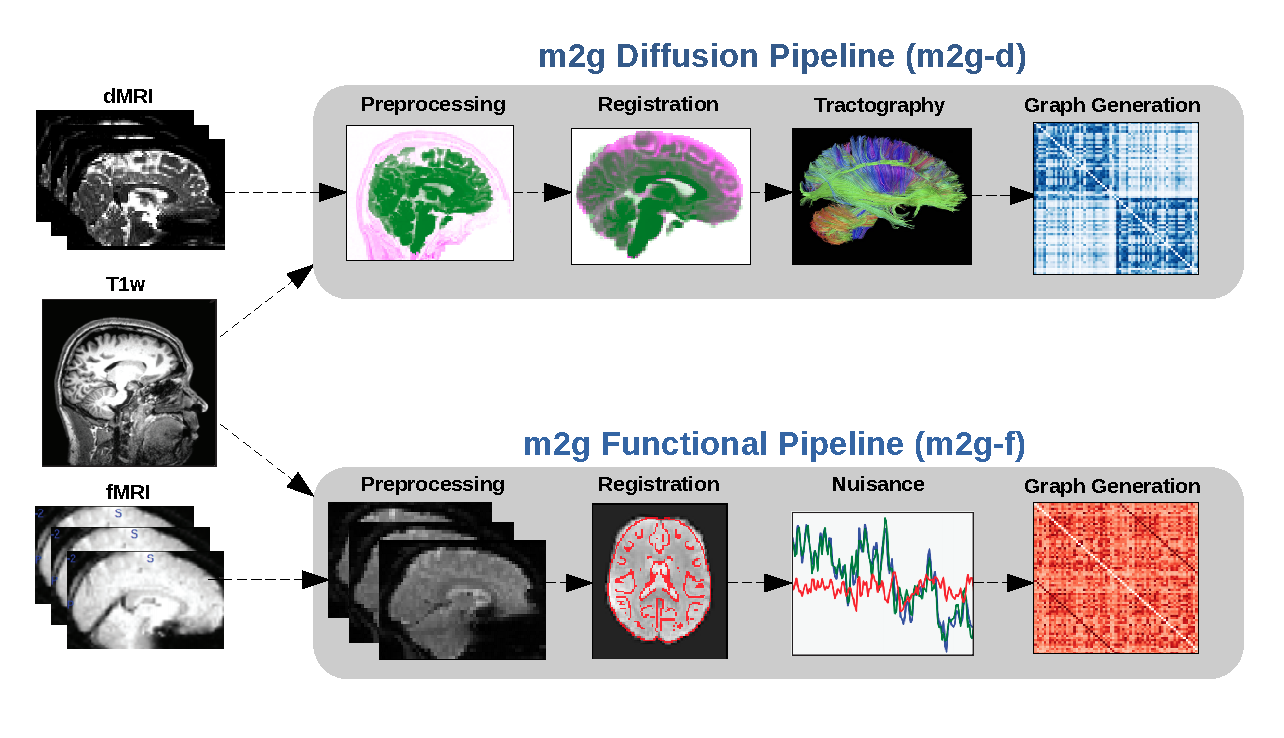
\includegraphics[width=1\textwidth]{figures/m2g/m2g_pipeline.pdf}
    \caption[The \texttt{m2g} pipeline has two sub-pipelines: \texttt{m2g-d} transforms Nifti-formatted dMRI data into sparse structural connectomes, and \texttt{m2g-f} organizes the data for processing by CPAC's functional pipeline that we developed here.]
    {\textbf{Individual Level Pipeline}
  The \texttt{m2g} pipeline has two sub-pipelines: \texttt{m2g-d} transforms Nifti-formatted dMRI data into sparse structural connectomes, and \texttt{m2g-f} organizes the data for processing by CPAC's functional pipeline that we developed here. Each sub-pipeline consists of four key steps, and each step generates both data derivatives and quality assurance figures to enable both qualitative assessments and quantitative comparisons. Detailed descriptions of the processes involved in each step can be found in the m2g Diffusion Workflow and m2g Functional Workflow sections.
}
	\label{fig:ndmgpipeline}
\end{figure*}


\subsection{The m2g Pipeline}

The \texttt{m2g} pipeline consists of two separate sub-pipelines: \texttt{m2g-d}, which processes diffusion-weighted MRI scans to estimate structural connectomes, and \texttt{m2g-f}, which processes BOLD functional MRI scans to estimate functional connectomes. While the \texttt{m2g-d} sub-pipeline is locally contained in \texttt{m2g}, \texttt{m2g-f} has been integrated into CPAC \cite{cpac} as a Nipype pipeline, \cite{nypipe} which is called during the processing of functional MRI data. While the code itself was developed by our group, and the performance is monitored for consistency between updates, the \texttt{m2g-f} sub-pipeline is hosted and maintained by the FCP-INDI organization. The steps involved in each of these sub-pipelines are further discussed in the Methods section. Due to the focus on ease of use and generalizability, \texttt{m2g} only requires the path of the BIDs ~\cite{bidspec} organized input directory, the output directory, and which of the pipelines is to be run (with other parameters able to be specified by the user). Through calling \texttt{m2g} with the simplest parameters:
\begin{verbatim}
                m2g --<type> <input_directory> <output_directory>
\end{verbatim}
where  \texttt{<type>} is either \texttt{dwi} for the diffusion pipeline, \texttt{func} for the functional pipeline, or \texttt{both} for when both pipelines should be run, \texttt{m2g} is able to estimate connectomes. We used the \texttt{m2g} pipeline to successfully estimate all of the connectomes used in this manuscript with data consisting of both functional and diffusion MRI nifti files of varying voxel resolutions and acquisition methods (see \texttt{DatasetInfo.pdf} in the Supporting Materials for further details). 
\texttt{m2g} is also able to process scans with non-isotropic voxels without issue due to the reslicing performed in both the \texttt{m2g-d} and \texttt{m2g-f} pipelines utilizing Dipy's reslice function with tri-linear interpolation ~\cite{dipy}. As reslicing an image to a different resolution results in the creation of new voxels with different intensity values, it may cause concern that there is significant change to  the information contained within the images and by extension the connectomes. However, it has been shown that such processing does not significantly change the information for both diffusion and functional MRI ~\cite{trilin1,trilin2}.

In addition to visual inspection of quality assurance (QA) figures generated after each step in the pipeline, we used the discriminability metric, which evaluates the fraction of measurements from the same individual that are closer to one another than they are to the measurement of any other individual~\cite{discriminability}, as a benchmark to the performance of \texttt{m2g} during development. The \texttt{m2g-d} pipeline was optimized on the Kirby21 dataset \cite{Kirby21}, while the \texttt{m2g-f} pipeline was optimized on both the Kirby21 and IBATRT \cite{ibatrt} datasets because they are commonly used for test-retest analysis. Both pipelines were then validated using data from the Consortium of Reliability and Reproducibility (CoRR), consisting of 35 different studies from nearly 20 different institutions around the world, spanning the Americas, Europe, and Asia~\cite{corr}. The CoRR data collection efforts were not harmonized, and all data (regardless of quality) were requested to be shared. This data repository was thus well-suited to test the robustness of our pipeline. Several additional open-access datasets from other repositories with different acquisition details, such as ABIDE~\cite{abide1, abide2}, were also processed with \texttt{m2g}.

The neuroparc repository of atlases, which we cultivated alongside \texttt{m2g}, was used as the main resource for the standardized parcellations used in \texttt{m2g}'s development ~\cite{neuroparc}. This repository served to consolidate atlases from a multitude of sources, each registered to MNI152 space at 1, 2, and 4 mm$^3$ voxel sizes~\cite{mni152}. Of the atlases listed there, 35 were used during the development of \texttt{m2g}. While neuroparc was developed in unison with \texttt{m2g}, the \texttt{m2g} pipeline is capable of utilizing any parcellation atlases provided by the user, provided it has been registered into MNI152 space~\cite{mni152}.

Due to the lack of gold standards to determine the accuracy of an estimated connectome, % meaning whether the relationships estimated from the MRI data are representative of the "ground truth" of the connections present in an individual's brain, 
certain forms of validation of the \texttt{m2g} pipeline are impossible. 
However, we have used surrogate metrics for QA to increase confidence in the outputs. For each MRI, \texttt{m2g} ran to completion while passing a basic QA metric consisting of (1) each connectome is a single connected component% edge values associated with every ROI
, (2) for all applicable datasets, discriminability values are above 0.7, (3) QA figures were generated successfully, (4) homophyly and homotopy observations are in agreement with literature. \texttt{m2g}'s ability to pass these metrics for validation shows its ability to be used widely, across a variety of datasets, including those leveraging older MRI technology.

To visually inspect consistency in estimated connectomes across the datasets, a distance-dependent group consensus structural connectivity graph was created. This method serves to prevent the observed trend of down-weighting long-range connections ~\cite{struct_consensus} in conventional averaging of connectomes and preserves the network properties seen in individuals. A similar graph was created for the functional MRI data, called a group-averaged functional connectivity matrix \cite{func_consensus}, which serves to minimize the effect of inconsistent correlations (Figure~\ref{fig:meancon}). The reproducibility of the estimated connectomes was tested using discriminability~\cite{discriminability}, and network statistics to determine that biological diversity, i.e. structural or functional properties unique to each subjects, and connectome plausibility were maintained.

%include something about passing to ranks?

\begin{figure*}%[t!]
	\centering
	%\includegraphics[width=0.74\textwidth]{./figs/dwi_func_connectome2.pdf}
	\includegraphics[width=.7\textwidth]{figures/m2g/figure2.pdf}
    \caption[Group consensus structural connectome from  \texttt{m2g-d} (blue) and group consensus functional  connectomes from \texttt{m2g-f} (red).]
    {\textbf{Group Consensus Connectomes}
  Group consensus structural connectome from  \texttt{m2g-d} (blue) and group consensus functional  connectomes from \texttt{m2g-f} (red), using the DKT parcellation method \cite{desikan2006automated}. Structural connectomes of the datasets appear qualitatively similar, with minor deviations particularly visible in the contralateral regions of the connectomes (nodes 0-40 and 41-80). Ipsilateral connectivity is consistently more dense than contralateral connectivity in structural connectomes \cite{ipsi-struct}. The functional connectomes appear qualitatively similar to one another. Homotopic correlation is consistently higher than ipsilateral and contralateral connectivity, which agrees with existing knowledge about functional correlation in the brain~\cite{Stark-ipsi,Biswal-ipsi,Zuo-ipsi}.
  }
	\label{fig:meancon}
\end{figure*}


\subsection{Validated Connectomes}
Connectomes were estimated by both \texttt{m2g-d} and \texttt{m2g-f} for 35 parcellations from the Neuroparc repository~\cite{neuroparc} (see \texttt{Parcellations.pdf} in Supporting Materials). As mentioned before, the "true" accuracy of estimated connectomes compared to the true functional and structural properties of individuals' brains is impossible to measure. Instead, we measure the reliability of the  \texttt{m2g} pipelines through the discriminability of each dataset (Figure \ref{fig:func_discrim}),  and evaluate validity through various proxies, including the amount of homophyly and homotopy between regions of interest (Figure \ref{fig:ipsi}), and manual inspection of extensive QA images generated during each major step of the pipelines (see Appendix for example Figures \ref{fig:diff_skull}-\ref{fig:func_motion}). The connectomes estimated by \texttt{m2g} consistently, regardless of parcellation method/dataset, had corresponding discriminability metrics above random chance and in certain conditions achieving optimal results. Analysis of the homophyly and homotopy from connectomes estimated by \texttt{m2g} were found to agree with well documented phenomena~\cite{ipsi-struct,Stark-ipsi,Biswal-ipsi,Zuo-ipsi}, and manual inspection of a random sampling of QA images found no major errors.

\begin{figure*}%[t!]
    \centering \offinterlineskip
    % \includegraphics[width=1\textwidth]{./figs/disc_heatmap_vert.pdf}
    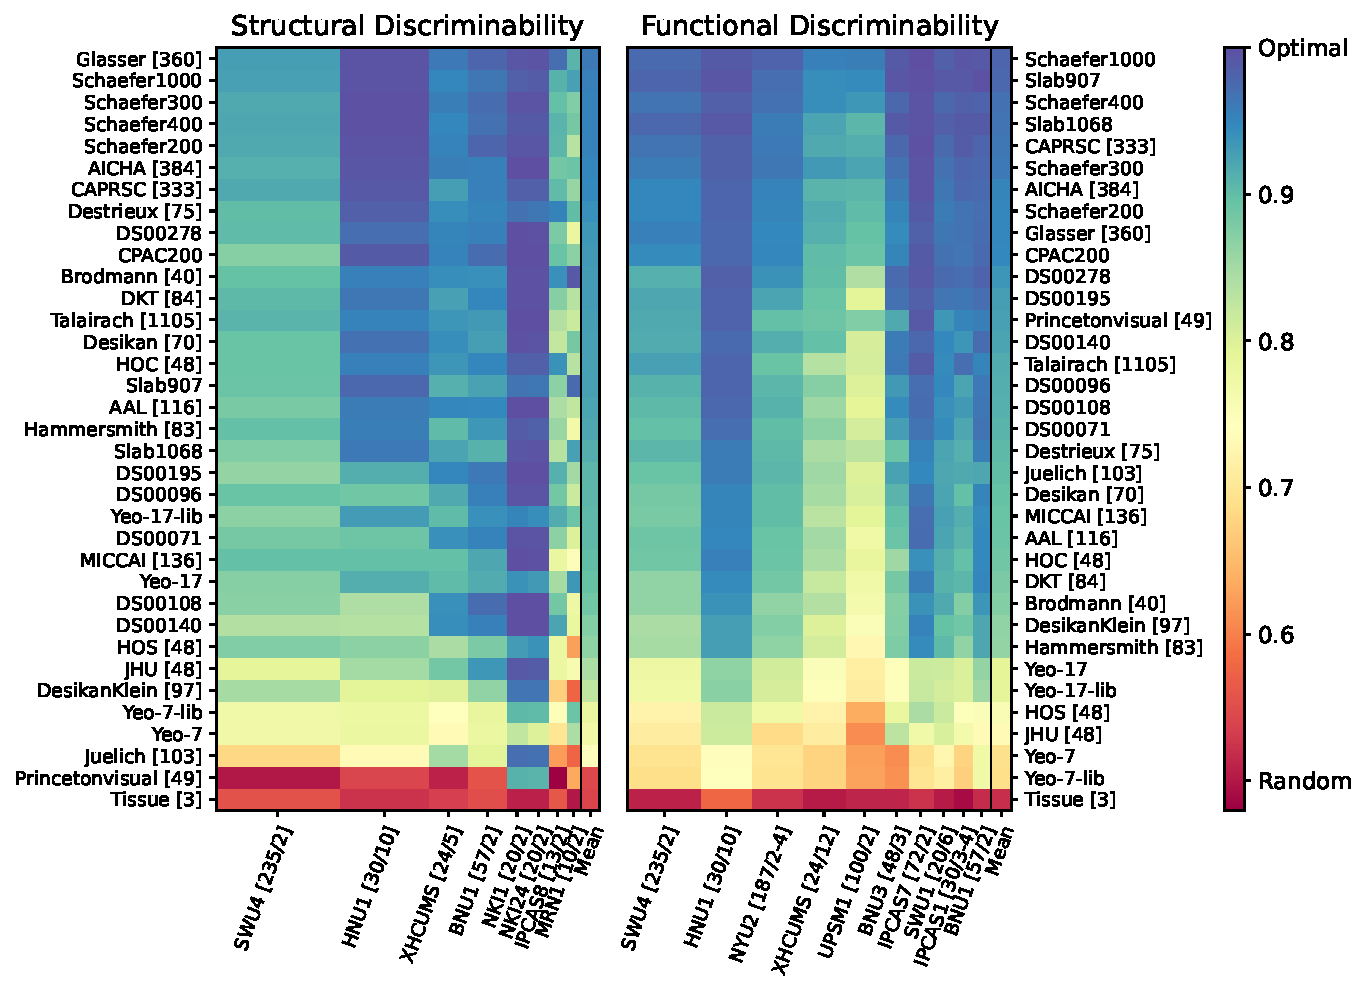
\includegraphics[width=1\textwidth]{figures/m2g/figure3.pdf}
    %\centering \includegraphics[width=0.85\textwidth]{./figs/func_heatmap_roi.pdf}
    \caption[Discriminability values from each applicable diffusion (left) and functional (right) MRI dataset.]{\textbf{Discriminability Results}
    Discriminability values from each applicable diffusion (left) and functional (right) MRI dataset. Relative row height denotes the relative size of the dataset. Rows, each representing a different parcellation, are organized from top to bottom by highest to lowest mean discriminability value. The mean discriminability value for each parcellation is displayed in the last column of both plots. The number of subjects/sessions is displayed next to the datasets' names in brackets and the number of ROI's in a given parcellation are shown in brackets if not mentioned in the parcellation name. Discriminability values for the structural connectomes was greater than 0.7 for the 32 of the 35 parcellations, while being robust to the number of scans per subject. Functional connectomes rarely had discriminability values lower than 0.7.}
    \label{fig:func_discrim}
\end{figure*}


\subsubsection{Discriminability}
Discriminability~\cite{discriminability}  was estimated for every dataset with multiple scans per subject (as reported in the Supporting Materials, which gives all of the individual numeric values). The closer to 1 the discriminability value of a processed dataset is, the more distinct the connectomes estimated from one individual's scans are from the connectomes of others. A discriminability value of one supports the estimated connectome capturing some unique functional or structural property for each of the subjects. The \texttt{m2g-d} pipeline estimated connectomes with discriminability values  greater than 0.7 for the 33 of the 35 parcellations (Figure~\ref{fig:func_discrim}, top). The discriminability measurements appear to be robust to the number of scans per subject, as can be seen with the SWU4 and HNU1 datasets (two scans per subject and ten scans per subject, respectively). In addition, \texttt{m2g-f} rarely estimated connectomes with discriminability values lower than 0.7 (Figure~\ref{fig:func_discrim}, bottom).


\subsubsection{Connectome Connectivity}
Because discriminability assesses the uniqueness of each individual's connectome, it does not guarantee that the connectome itself is biologically meaningful. 
To address this issue, we analyzed the prominence of  different categories of connections---ipsilateral versus contralateral and   homotopic versus heterotopic---using the connectomes estimated from three unique parcellations. To analyze homotopic connections, we chose the DKT~\cite{desikan2006automated}, AAL~\cite{AAL}, and Hammersmith~\cite{Hammersmith} parcellations, due to their symmetric ROI placement (i.e. each ROI on the left hemisphere had a matching ROI on the right). For the structural connectomes, the percentage of total edges which belonged to each network were analyzed, while the absolute Pearson's correlation value~\cite{pearson} calculated by CPAC was used for the functional connectomes. The results coincided with well-documented phenomena regarding structural and functional relationships \cite{ipsi-struct,Stark-ipsi,Biswal-ipsi,Zuo-ipsi}. Namely, structural connectomes had significantly more ipsilateral than contralateral connections, while functional connectomes had significantly stronger homotropic correlations than heterotropic, either ipsilaterally or contralaterally (Figure \ref{fig:ipsi}). 
% The results coincided with well documented  phenomena regarding structural and functional relationships \cite{ipsi-struct,Stark-ipsi,Biswal-ipsi,Zuo-ipsi}.

\begin{figure}
    \centering
    %\includegraphics[width=1\textwidth]{figs/connectome_connect.pdf}
    %\includegraphics[width=1\textwidth]{figs/connectome_connect3.pdf}
    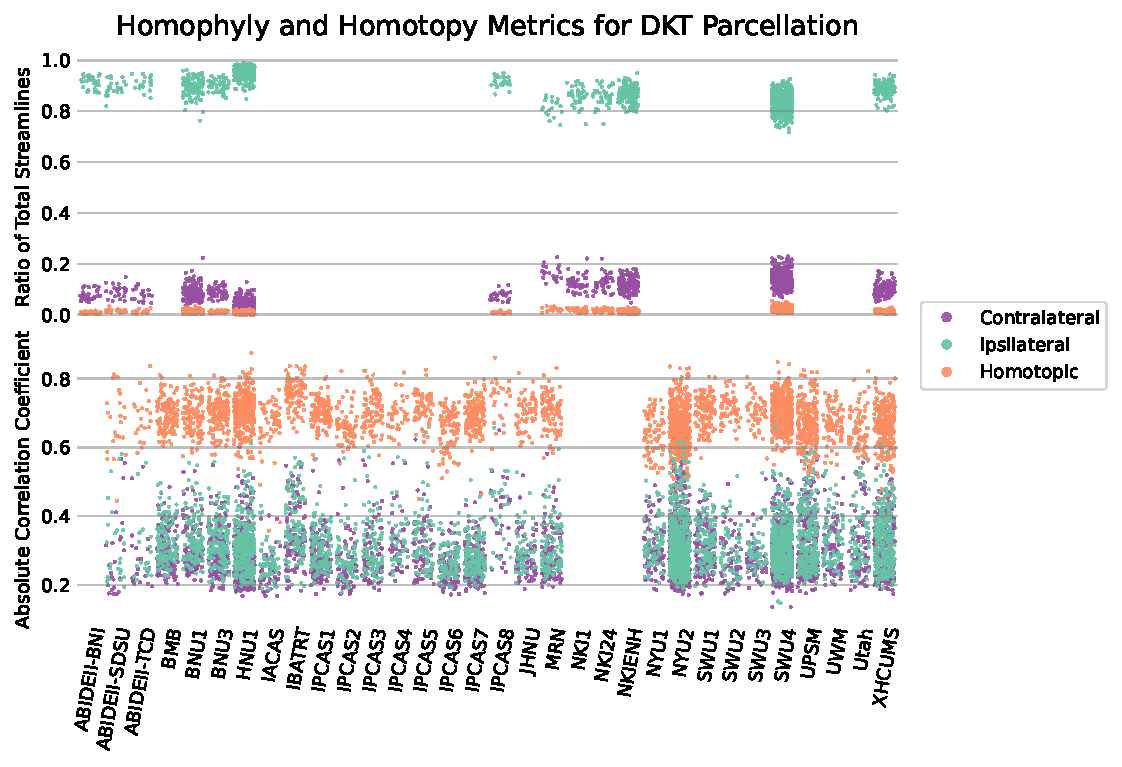
\includegraphics[width=1\textwidth]{figures/m2g/figure4.pdf}
    \caption[Analysis of the edge weights of both structural (top) and functional (bottom) connectomes estimated using the DKT parcellation method.]{\textbf{Connectome biological plausibility results} Analysis of the edge weights of both structural (top) and functional (bottom) connectomes estimated using the DKT parcellation method. For the structural connectomes, the mean of the percentage of streamlines observed between ipsilateral, contralateral, and homotopic ROIs was recorded and plotted for each scan. Mean Pearson correlation coefficients between ipsilateral, contralateral, and homotopic ROIs was plotted for functional connectomes. A consistent significantly higher ratio of ipsilateral connections was observed across parcellation methods for structural connectomes, as well as a higher correlation between homotopic ROIs across parcellation methods in functional connectomes.}
    %Put in mean and standard deviation for each of these statements.
    \label{fig:ipsi}
\end{figure}


\subsubsection{Reproducibility}
In the \texttt{m2g} pipeline, each processing procedure may introduce bias or noise in the estimated connectome. The randomized seed placement which takes place in the tractography step of the \texttt{m2g-d} pipeline, and the registration of the functional MRI data onto the T1-weighted image and the T1-weighted image onto the diffusion MRI data for \texttt{m2g-f} and \texttt{m2g-d}, respectively, serve as potential vectors for noise. To test the reproduciblity of \texttt{m2g}, we estimated connectomes for a subset of scans multiple times. Using a subset of five scans from each dataset, we used \texttt{m2g} to estimated connectomes five times per scan, using the same default parameters. The resulting connectomes were then treated as unique, with each set belonging to the same subject. Discriminability metrics were then calculated to determine whether the unique qualities of the individual scan were preserved. For all subsets, discriminability values of 1 were recorded for all parcellations for both the functional and structural connectomes. This supports the robustness of \texttt{m2g} to any bias or noise, as the unique properties of each subject are significant enough not to be altered. Additional testing using Spearman's rank correlation found that the repeated connectomes had a coefficient greater than 0.98 for all parcellations.

%With respect to programmatic reproducibility, m2g fully supports execution via the Docker container platform. Container images are generated and uploaded to a public repository for each new version of m2g. These containers are released with version-controlled libraries for m2g and all its dependencies, maximizing run-to-run reproducibility in an easy way. This helps to address the widespread lack of reporting of specific software versions and the large variability of software, which threaten the reproducibility of MRI analyses \cite{}. The Docker image for m2g can be found at \url{https://neurodata.io/m2g/}%\url{https://hub.docker.com/r/neurodata/m2g}.

\subsubsection{Quality Assurance Outputs}
Quality assurance images were created by \texttt{m2g} at each of the significant steps in both the \texttt{m2g-d} and \texttt{m2g-f} pipelines (Figure \ref{fig:ndmgpipeline}) for easy determination of erroneous results. The QA figure formats were chosen for clarity and minimal image analysis expertise requirements in order to detect any potential errors. A random sample of the QA images from 15 estimated connectomes per dataset were visually inspected and found no significant issues. Samples of the output QA images can be found in the Appendix. Documentation for each of the QA figures generated by \texttt{m2g} can be found at \url{https://neurodata.io/mri/}. %\url{https://github.com/neurodata/m2g}.

\subsection{Low Resource and Time Requirement}
\begin{figure*}%[t!]
	\centering
    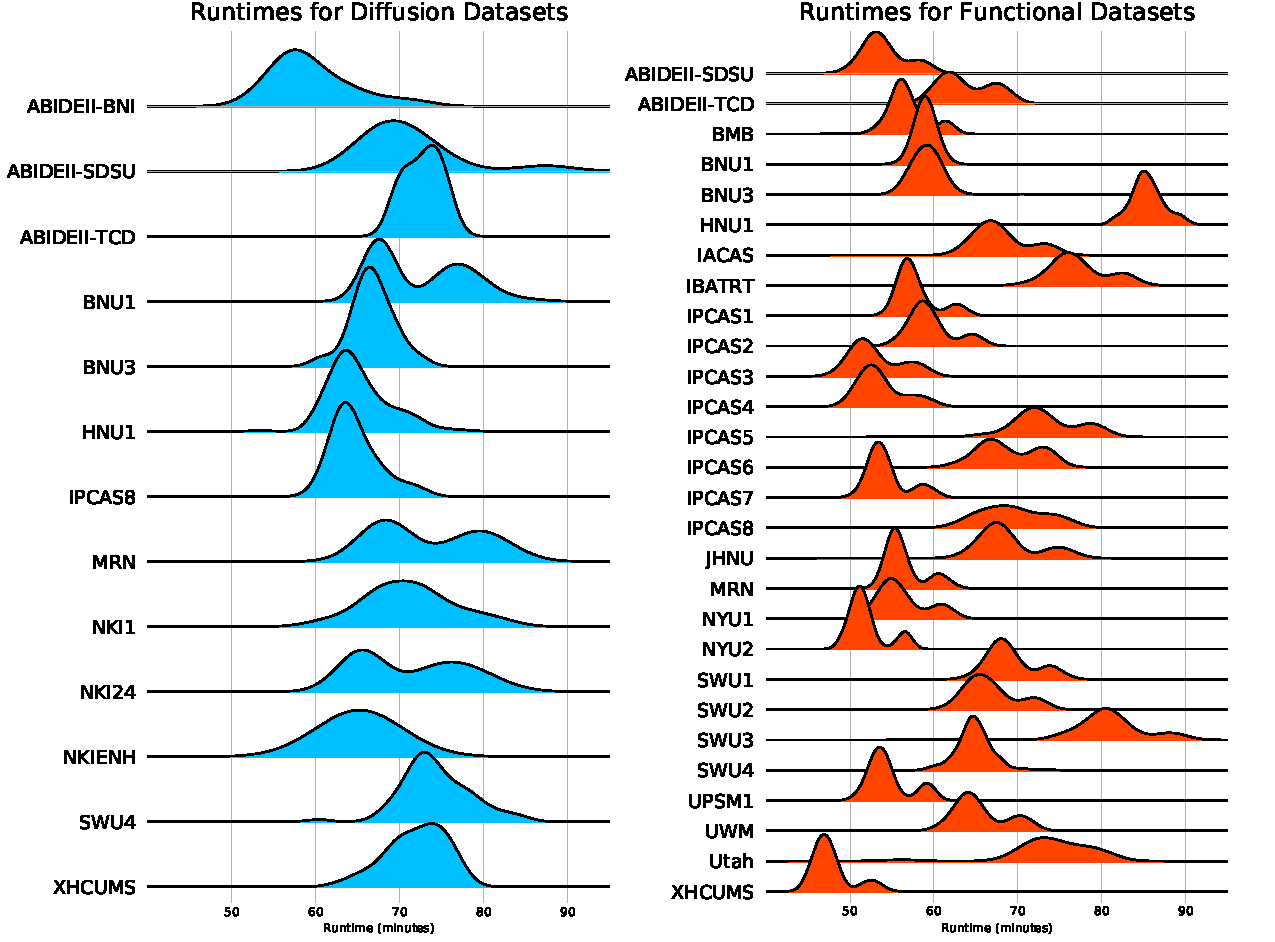
\includegraphics[width=0.9\textwidth]{figures/m2g/seperated_joyplot.pdf}
    \caption{\textbf{Runtimes for Diffusion and Functional datasets}
    Amount of time, in minutes, it took for \texttt{m2g} to generate a connectome for each of the scans in the datasets using the 35 brain parcellations. Computation time for diffusion datasets (blue) and functional datasets (red) varied based off of size and resolution of the input MRI files. In these time estimates, \texttt{m2g} was run utilizing 3 CPUs in parallel and at least 16 GB of RAM available.
    }
	\label{fig:runtime}
\end{figure*}
Computational expediency and resource efficiency were two key reasons we developed \texttt{m2g}. While the required resources for running \texttt{m2g} varies according to the data, the datasets mentioned in this paper could be processed by \texttt{m2g} with approximately 16 GB of RAM and 1 CPU core. If more resources are available, \texttt{m2g} is capable of utilizing multiple CPUs at the same at various points throughout the pipeline, such as registration and graph generation, to reduce runtime. While estimating the connectomes used in this manuscript, we recorded the time required for \texttt{m2g} to successfully analyze each of the scans used in the discriminability calculations (Figure \ref{fig:runtime}). The optimal configuration of resources for our purposes required 3 CPUs and 16 GB of RAM. When tested using 1 CPU, \texttt{m2g-d} took less than 120 minutes to complete the connectome creation using 35 parcellations for a given dMRI scan. The \texttt{m2g-f} pipeline likewise took less than 110 minutes to generate the set of connectomes. Additional CPUs were found to significantly increase the RAM requirements of the \texttt{m2g-f} pipeline, due to the configuration of CPAC.

%Computational expediency and resource efficiency were  key  reasons to develop m2g. While the required resources for running m2g varies according to the data, the datasets mentioned in this paper could be  processed by m2g with approximately 16 GB of RAM and 1 CPU core. If more resources are available, m2g is capable of utilizing multi-threading at various points throughout the pipeline to reduce run-time at the cost of increased RAM requirements. Runtimes for the files of each dataset when m2g was used with 3 CPUs and 16 GB of RAM (Figure \ref{fig:runtime}).

\section{Discussion}
The \texttt{m2g} processing pipeline was created to both efficiently analyze diffusion and functional MRI scans and lower the barrier for entry to connectomics. It was developed to excel at three key aspects: ease of use, biological veracity, and computational reproducibility. We believe \texttt{m2g} to be a success with respect to these three aspects.

Attesting to its ease of use, all datasets referenced in this manuscript were run through \texttt{m2g} with the default parameters and minimal user input, resulting in the successful generation of connectomes for each scan. This was true across a range of acquisition properties of the MR images and with modest computational resources: less than two hours for each scan using 16 GB of RAM and 3 CPUs and no intra-pipeline additional parallel processing steps. In addition, \texttt{m2g} requires very minimal user input: only the input/output locations, pipeline type, and acquisition method (for fMRI data).  As such, the pipeline is an easy tool for researchers and clinicians without extensive computer science experience or resources. Also, \texttt{m2g} produces comprehensive visual reports to analyze processing output: we designed the QA figures to easily visually determine whether the pipeline has successfully processed the provided data. With the emphasis on color coordination and concise figure generation, many issues in the preprocessing and registration process is easily visible. All QA figures are clearly labeled and placed in the same directory location relative to the output, regardless of pipeline being used, with detailed explanations found at \url{http://m2g.io}.

%Preservation of Biological Veracity
We assessed \texttt{m2g}'s ability to produce biologically plausible and realistic data using multiple approaches.  First, and most simply, we determined that there was a path from each ROI to each other ROI, i.e., that the brain was connected, which we know to be generally true. Second, our visual inspection of output QA figures showed no obvious abnormalities that would negatively effect the accuracy of the connectome. Third, we computed the discriminability for each dataset. Discriminability surpassed statistical tests of random chance for essentially all parcellations across datasets. In fact, the majority of the 35 parcellation methods used in this analysis resulted in discriminability values above 0.8 (Figure \ref{fig:func_discrim}). Fourth, we assessed the relative fraction of ipsilateral versus contralateral, and homotopic versus heterotopic connections. 
% Analysis of the connection ratios in the generated connectomes also supported the biological "truth" of the connectomes. 
Results were consistent with current knowledge about the anatomical and functional realities of neuro-typical brains~\cite{ipsi-struct,Stark-ipsi,Biswal-ipsi,Zuo-ipsi}. More specifically, the prominence of ipsilateral connections in structural connectomes, and the prominence of homotopic correlations in functional connectomes (Figure \ref{fig:ipsi}).

%Transparency of Results
Our focus on computational reproducibility manifested through \texttt{m2g} being open source and fully supporting execution via the Docker container platform. From version to version of \texttt{m2g}, prospective users do not need to worry about reproducibility issues due to dependency issues as container images are generated and uploaded to a public repository for each new version of m2g. These containers are released with version-controlled libraries for m2g and all its dependencies, maximizing run-to-run reproducibility in an easy way. The Docker image for m2g can be found at \url{https://neurodata.io/mri/}. We also confirmed within version computational reproducibility for \texttt{m2g} through the re-estimation of connectomes, which showed optimal discriminability values and Spearman's rank correlation greater than 0.98 for essentially all parcellations across datasets.


%Vectors for Improvement
The design criteria for \texttt{m2g} required certain trade-offs in performance to increase the generalizability of input data. With the strength of pipeline flexibility and minimal required user input still being paramount, \texttt{m2g} could be improved along several dimensions. First, recent advances in registration \cite{lddmm} and tractography \cite{probtrackx} could be incorporated. Second, several more sophisticated batch effect strategies have been successfully employed in dMRI data \cite{Fortin2017-dm,bridgeford_batch_paper}. Such strategies could possibly help here as well, especially if they are modified appropriately to work on binary graphs \cite{Leek2007}. Third, \texttt{m2g} may under-perform for particular populations (e.g., infants), for brains that show nonstandard structures such as tumors, resected regions, lesions, or other species (e.g., non-human primates~\cite{xu2020cross}).  Inclusion of the ability to supplement the standard MNI152 reference images and parcellations with ones relevant to nonstandard brain structures could drastically expand the populations \texttt{m2g} could process. This would be particularly interesting as a means to adapt the workflow to data collected from rodents and nonhuman primates in the future.

%Future
Because the methods developed during the creation of \texttt{m2g} are open-source and easy to use, and the data are open-access, the continual development of the pipeline and assessment of the connectomes generated is ready for outside collaboration. Due to the well-commented and modular code, modification is straightforward for python users. Along with the ease of use, a boon for the wider adoption of \texttt{m2g} is the plethora of connectomes created as a byproduct of its development. These connectomes are open-access and available from our website, \url{https://neurodata.io/mri/}.

\section{Methods}
\subsection{Data}
The \texttt{m2g} pipelines were validated through the processing of the majority of data from the Consortium of Reliability and Reproducibility (CoRR). The CoRR data consists of 36 different studies from nearly 20 different institutions around the world, spanning the Americas, Europe, and Asia \cite{corr}. The CoRR data collection efforts were not harmonized, and all data (regardless of quality) were shared. Thus, these collections are well-suited to test the robustness of any pipeline. In addition to the CoRR data, we also used \texttt{m2g} to process several additional open-access data collections with complementary acquisition parameters (see Supporting Material \texttt{DatasetInfo.pdf}).
Using this collection of MRI data, \texttt{m2g} pipeline development and parameter selection prioritized the maximization of discriminability scores across all datasets, while also focusing on limiting resource requirements.

\subsection{m2g Input}
The input required to run the \texttt{m2g} pipeline depends on whether functional and/or diffusion MRI data is being analyzed. The required inputs for either pipeline are:
\begin{itemize}
    \item A T1-weighted anatomical scan, either an uncompressed or gzipped nifti file
    \item \textbf{\texttt{m2g-d}:} 
    \begin{itemize}
        \item A diffusion-weighted MRI file, either an uncompressed or gzipped nifti file
        \item b-value and b-vector parameter files (.bval and .bvec file types)
    \end{itemize}
    \item \textbf{\texttt{m2g-f}:} \begin{itemize}
        \item A functional MRI file, either an uncompressed or gzipped nifti file
        \item The TR value (in seconds) and acquisition method used for the functional scan
    \end{itemize}
\end{itemize}
The directory containing the input data must be BIDS formatted \cite{bidspec}. Both the \texttt{m2g-d} and \texttt{m2g-f} pipelines can be run independently or on the same dataset, provided the required data files are available. Which parcellation(s) to be used in the connectome creation can be specified by the user, whether they be unique files stored locally or from the neuroparc repository~\cite{neuroparc}. If no parcellations are present, then \texttt{m2g} will pull from the neuroparc repository and run all available parcellations.

\subsection{m2g Diffusion Workflow}
The \texttt{m2g} diffusion pipeline leverages existing open source tools, including the fMRI Software Library (FSL) ~\cite{fsl1, fsl2, fsl3}, Dipy~\cite{dipy}, the MNI152 atlas~\cite{mni152}, and a variety of parcellations defined in the MNI152 space~\cite{neuroparc}. The pipeline consists of five major steps: (1) Preprocessing, (2) Registration, (3) Tensor estimation, (4) Tractography, and (5) Graph generation.
All algorithms used throughout the pipeline requiring hyper-parameter selection were initially set to the suggested parameters, and optimized on the subset of CoRR datasets. The output of each processing stage includes data derivatives and QA figures to enable individualized accuracy assessments. The QA figures at each major step include cross-sectional images at different depths in the three canonical planes (sagittal, coronal, and axial) of images or overlays. Figure~\ref{fig:ndmgpipeline} provides a schematic of the individual-level analysis.

\subsubsection{Preprocessing}
The input diffusion MRI data is first eddy-corrected using FSL's eddy\_correct \cite{dipy} program with the default parameters. This program was chosen as newer eddy functions either require substantially longer to run or rely on GPU acceleration, an additional resource requirement which would reduce the accessibility of \texttt{m2g}. The associated bvec and bval files are then checked for any errors and, if necessary, corrected using Dipy's read\_bvals\_bvecs function \cite{dipy} into a usable format. The b-vectors are then normalized, making sure to not alter the b-vector if its associated b-value is 0.

The eddy-corrected dMRI file then has its orientation checked, and if not already oriented in RAS+ coordinate space, nibabel's as\_closest\_canonical ~\cite{nibable} is used for the reorientation. The b-vectors are also reoriented to RAS+ if necessary using default parameters. The dMRI file is then resliced to the desired voxel size (specified by the user, with a reasonable default of 2mm$^3$ if not specified) using Dipy's reslice function with trilinear interpolation\cite{dipy}.

The T1 weighted MRI file (T1w) is also reoriented into RAS+ format using as\_closest\_canonical and similarly resliced, if necessary, into the desired voxel size using Dipy's reslice function \cite{dipy} with default parameters. The resulting image is then skull-stripped using AFNI's 3dSkullStrip function ~\cite{AFNI} with the surface density parameter set to 30, resulting in an anatomical image with all non-neuronal structures removed.

\subsubsection{Registration}
From the skull-stripped T1w anatomical file, three probability masks are generated for the grey matter, white matter, and cerebral spinal fluid regions of the brain using FSL's fast function \cite{fsl1, fsl2, fsl3} using default parameters. The white matter mask is then used to create another mask of just the outer edge of the white matter area using FSL's fslmaths \cite{fsl1, fsl2, fsl3}. Using FSL's flirt function \cite{fsl1, fsl2, fsl3}, an initial linear registration is made for the anatomical image to the reference MNI152 template in MNI space. An initial attempt is made for non-linear registration of the T1w image to the MNI template, using the affine transformation matrix previously created by the linear registration as a starting configuration. If it is not successful and throws an error, linear registration is used. Using FSL's fnirt function \cite{fsl1, fsl2, fsl3}, the nonlinear warp coefficients/field is generated to register the T1w image onto the reference MNI image. FSL's invwarp function \cite{fsl1, fsl2, fsl3} is then used on the coefficients/field to get the field for registering the reference MNI image onto the T1w image. However, if the nonlinear registration fails, then the linear registration affine transformation matrix for T1w to MNI is used and inverted using FSL's convert\_xfm \cite{fsl1, fsl2, fsl3}.

FSL's flirt is then used for calculating the boundary-based registration (BBR) of the dwi image onto the T1w image, using 256 bins and 7 degrees of freedom. The resulting transformation matrix is inverted and used with a mutual information cost function in flirt to generate an image of the anatomical image registered to the dwi image. Using fslmaths, binary ventricle and corpus callosum masks in MNI space are generated. Along with the previously generated grey matter, white matter, and cerebral spinal fluid masks, flirt is used to register the masks to dwi space. A grey matter/white matter boundary binary mask is then made using fslmaths, which denotes the approximated boundary between the two tissue types across the entire brain, for later seed propagation in the tractography stage of the pipeline.

Finally, the parcellation files to be used in the graph generation are reoriented using nibabel's as\_closest\_canonical function into RAS+, where they are resliced to the desired voxel size using Dipy's reslice function. They are then registered from MNI to dwi space using the previously calculated transformation matrices, utilizing FSL's flirt function and the ''nearest neighbor'' cost function.

\subsubsection{Tractography}
Seeds are generated along the grey matter/white matter boundary mask of the registered brain using a custom python script, where the number of seeds per voxel on the mask can be specified by the user. The seed locations and dwi image are then used in conjunction with Dipy tractography functions \cite{dipy} in order to generate a series of non-directional streamlines spanning the image. \texttt{m2g} offers deterministic or probabilistic tractography, Constrained Spherical Deconvolution (CSD) or Constant Solid Angle (CSA) reconstruction methods, and particle filter or local tracking. Regardless of the tractography settings specified, the resulting series of streamlines is output and saved to a trk file for use in graph generation.

\subsubsection{Graph Generation}
For each parcellation being analyzed, each streamline is converted into voxel coordinates and analyzed for overlap with any of the regions specified by the parcellation. \texttt{m2g} does not determine the direction of a given streamline, making its connectome and resulting graph undirected. If a streamline overlaps with a given region for more than 2mm, it is considered an intersection. The number of streamlines intersecting a given region and the other regions they also intersect with are recorded and tabulated in the form of a weighted edgelist. In this edgelist format each unique region of interest on the parcellation, marked by a unique intensity value, is considered a node whose edge weight is the number of streamlines that connect it to another region. For example, if a streamline intersects two or more regions in the parcellation (region A, region B, and region C) the weight of the edges AB, AC, and BC is increased by one. In this sense, the order through which the streamline intersects is not important. The resulting edgelist is saved in the form of a csv file, and an accompanying adjacency matrix of the normalized edgelist is also saved. A unique edgelist will be made for each parcellation specified by the user.

\subsection{m2g Functional Workflow}
The \texttt{m2g-f} pipeline was constructed starting with the optimal processing pipeline identified in Wang et. al~\cite{discriminability} using CPAC~\cite{cpac}. The CPAC pipeline utilizes existing open source tools, including FSL~\cite{fsl1,fsl2,fsl3}, the MNI152 atlas~\cite{mni152}, and a variety of parcellations defined in the MNI152 space \cite{neuroparc}. The functional pipeline consists of four major steps: (1) Preprocessing, (2) Registration, (3) Nuisance correction, and (4) Graph generation.

\subsubsection{Preprocessing}
The \texttt{m2g-f} pipeline in CPAC uses AFNI's SkullStripping function \cite{AFNI} with a variable shrink factor between 0.4 and 0.6 over 250 iterations with nearest neighbor interpolation to eliminate all non-neuronal structures from the anatomical image. The resulting anatomical file is resampled to the desired resolution voxel size using FSL's FNIRT \cite{fsl1, fsl2, fsl3}. Slice timing correction is then performed using AFNI's 3dTshift \cite{AFNI}, utilizing the TR value and scan acquisition method provided by the user. The resulting image is then motion corrected using AFNI's 3dvolreg, aligning all images to the first image in the functional MRI's timeseries.

\subsubsection{Registration}
Nonlinear boundary based registration of the preprocessed fMRI and anatomical images are performed in order to transform them into MNI152 space. The MNI152 6th generation anatomical reference image \cite{mni152} is used in this registration process, as it is FSL's preferred image. The functional image is then registered to the anatomical scan using FSL bet \cite{fsl1, fsl2, fsl3} with BBR. FSL's standard white matter, grey matter, and cerebral spinal fluid masks are then registered onto the functional image using FSL's FAST thresholding, resulting in segmentation tissue masks. The specified atlases that are going to be used in the connectome generation are also registered to the functional space using FSL's FLIRT function.

\subsubsection{Nuisance Correction}
Nuisance correction of the functional image is performed using the component based noise correction (CompCor) method. Using ''noise ROIs'', or areas of white matter and cerebral spinal fluid whose intensity values are unlikely to be modulated by neural activity, physiological noise can be isolated\cite{compcor}.Based on this assumption, physiological noise in gray matter regions can be corrected for by regressing out principal components from noise ROIs. CompCor uses the previously registered white matter and cerebral spinal fluid masks (csf) in order to determine noise ROIs. A principal component analysis is applied using the top five components of the white matter and csf to characterize the times series data from the noise ROIs. Significant principal components are then introduced as covariates in a general linear model as an estimate for the physiological noise single space. Polynomial Detrending is also performed to remove linear or quadratic trends in the timeseries, likely from changes in scanner heat or subject movement. After nuisance regression, frequency filtering occurs on the functional data using a bandpass filter from 0.01 Hz to 0.1 Hz to account for low-frequency drift and high-frequency noise.

\subsubsection{Graph Generation}
With the anatomical files and atlases registered to the functional image, the estimation of the functional connectomes for each atlas can occur. For each ROI, the timeseries of the average of all voxels within the ROI at each collection time point is calculated. This timeseries is then used to calculate the Pearson's correlation coefficient \cite{pearson} between each pair of ROIs. The functional connectome is then rank-transformed by replacing the magnitude of the correlation with its relative rank, from smallest to largest \cite{discriminability}. The resulting adjacency matrix of correlations is then saved, along with an edgelist file containing the same information.

\subsection{Validation of m2g on Diverse Data}
\subsubsection{Discriminability}
To evaluate a method’s reliability, Wang et al. \cite{discriminability} developed a metric called “discriminability” that quantifies the fraction of measurements from the same individual that are closer to one another than they are to the measurement of any other individual. Discriminability, as seen in Equation (4.1), describes the probability that two observations within the same class are more similar to one another than two observations belonging to a different class:
\begin{equation}
D=P(||a_{ij}-a_{ij'}|| \leq ||a_{ij}-a_{i'j'}||)
\end{equation}
In the context of validation of \texttt{m2g}, each connectome is converted into a ranked vector, assigning each edge a weight between 0 and 1 from smallest to largest, and compared. This means that each connectome $a_{ij}$, in a test-retest dataset is first compared to other connectomes belonging to the same subject, $a_{ij'}$, and then to all connectomes belonging to other subjects, $a_{i'j'}$. A perfect discriminability score is 1, meaning that for all observations within the dataset, each connectome is more alike to connectomes from the same subject than to others. Optimizing \texttt{m2g} with respect to discriminability enables us to minimize the upper-bound on error for any general downstream inference task.
The discriminability score for the multitude of datasets run through the default settings of \texttt{m2g} were recorded (see Supporting Material \texttt{DiscrimNumbers.xlsx}). 
The average discriminability over all scans was approximately 0.85 for dMRI data and approximately 0.8 for fMRI data.

\subsubsection{Connectome Connectivity}
While discriminability may determine the extent that \texttt{m2g} preserves the unique properties of a given MRI scan, additional care must be taken to determine whether the connectomes generated by \texttt{m2g} conform with basic neurological phenomena. One way to do this involves observation of either the physical or functional connections between different regions of the brain. Three simple categories for these regions are ipsilateral (connections that stay within the left or right hemispheres), contralateral (across hemispheres), or homotopic (from one region of the brain to the same region on the other hemisphere).
Using the edge weights from the structural connectomes generated by \texttt{m2g}, the percentage of edges that fell into each of the three connection types was calculated, and the mean and standard deviation were found for each dataset. This process was performed for three parcellations which had clearly-defined homotopic regions of interest, namely the DKT, Hammersmith, and AAL atlases. For the functional connectomes generated, the Pearson's correlation between regions of interest was used as a metric. The mean and standard deviation of each of the three connection types was found for each dataset (Figure \ref{fig:ipsi}). 

%\subsubsection{Reproducibility}
%In order to measure the extent to which m2g's repeated processing of data resulted in similar results, a subset of scans selected for repeated analysis. A total of 5 functional/diffusion weighted scans from each dataset was selected. Connectomes were estimated from each of the scans 5 times. Each connectome was then converted into a vector of edgeweights or Pearson correlations. To determine the consistency, the Spearman correlation between the connectomes from each scan was then calculated using the equation:
%For a sample size $n$, the $n$ raw scores $X_i,Y_i$ are converted to ranks $rg_{X_i}$, $rg_{Y_i}$, and $r_s$ is computed as:
%\begin{equation}
%    r_s = \rho_{rg_X,rg_Y} = \frac{cov(rg_X,rg_Y)}{\sigma_{rg_X}\sigma_{rg_Y}}
%\end{equation}
%where $\rho$ denotes the usual Pearson correlation coefficient, but applied to the rank variables. $cov(rg_X,rg_Y)$ is the covariance of the rank variables, and $\sigma_{rg_X}$ and $\sigma_{rg_Y}$ are the standard deviations of the rank variables.


\section{Ethical Compliance}
We complied with all relevant ethical regulations. This study reused publicly available data acquired at many different institutions. Protocols for all of the original studies were approved by the corresponding ethical boards.

\section{Software Availability}
All of our processed data is available from our website, \url{http://m2g.io}, and has been deposited into our public github repository, \url{https://github.com/neurodata/m2g}, and published with a DOI, \url{https://doi.org/10.5281/zenodo.1161284}, under the Polyform License. Detailed documentation can be found at \url{https://docs.neurodata.io/m2g/}.

\section{Data Availability}
The data derivatives that support the findings of this study are available from our website, \url{http://m2g.io},  under a (ODC-By) v1.0 license.


\section{Supplementary Figures}

\section{Appendix}

\begin{figure}[b!]
    \centering
    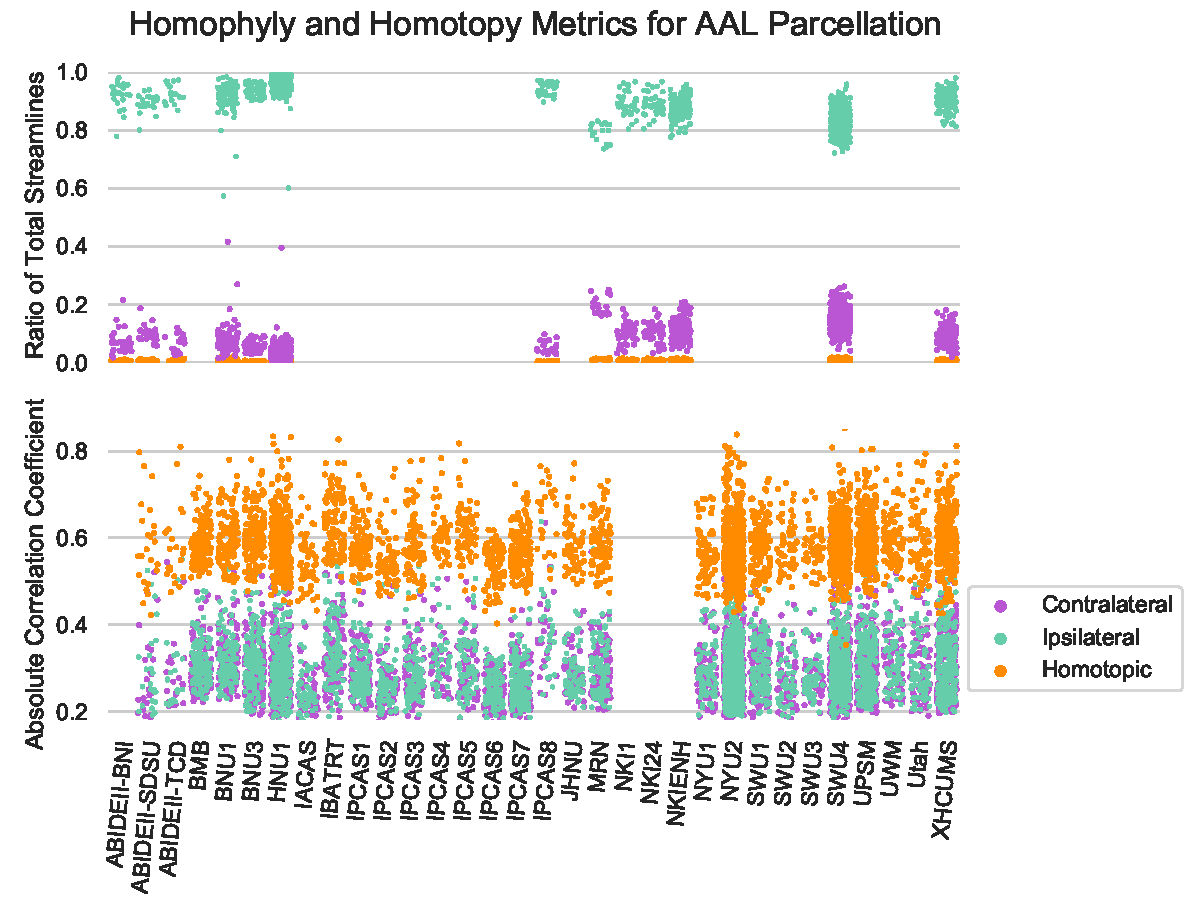
\includegraphics[width=1\textwidth]{figures/m2g/ipsi_aal.pdf}
    \caption[Analysis of the edge weights of both structural (top) and functional (bottom) connectomes estimated using the AAL parcellation method.]{\textbf{Connectome biological plausibility results} Analysis of the edge weights of both structural (top) and functional (bottom) connectomes estimated using the AAL parcellation method. For the structural connectomes, the mean of the percentage of streamlines observed between ipsilateral, contralateral, and homotopic ROIs was recorded and plotted for each scan. Mean Pearson correlation coefficients between ipsilateral, contralateral, and homotopic ROIs was plotted for functional connectomes. A consistent significantly higher ratio of ipsilateral connections was observed across parcellation methods for structural connectomes, as well as a higher correlation between homotopic ROIs across parcellation methods in functional connectomes.}
    \label{fig:ipsi_aal}
\end{figure}

\begin{figure}[h!]
    \centering
    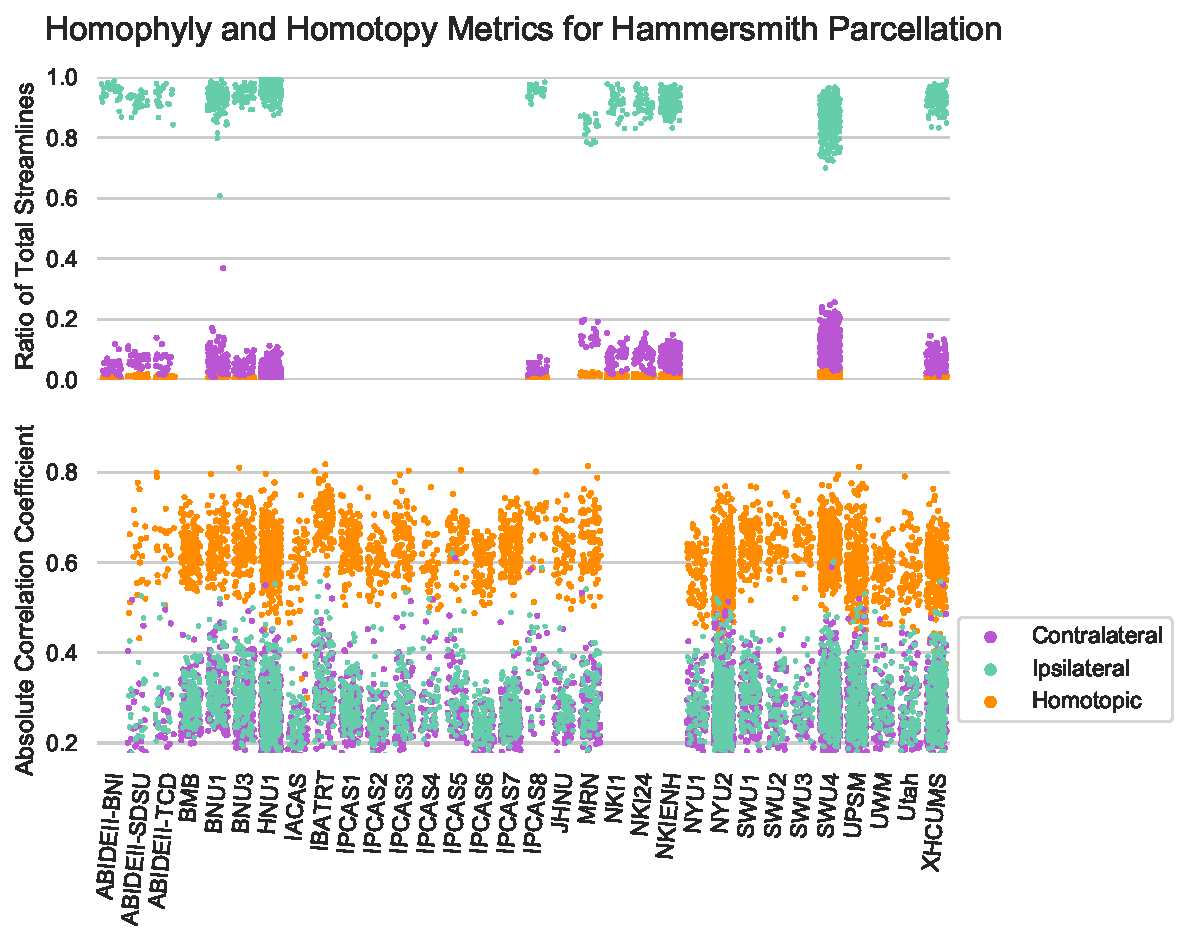
\includegraphics[width=1\textwidth]{figures/m2g/ipsi_hammer.pdf}
    \caption[Analysis of the edge weights of both structural (top) and functional (bottom) connectomes estimated using the Hammersmith parcellation method.]{\textbf{Connectome biological plausibility results} Analysis of the edge weights of both structural (top) and functional (bottom) connectomes estimated using the Hammersmith parcellation method. For the structural connectomes, the mean of the percentage of streamlines observed between ipsilateral, contralateral, and homotopic ROIs was recorded and plotted for each scan. Mean Pearson correlation coefficients between ipsilateral, contralateral, and homotopic ROIs was plotted for functional connectomes. A consistent significantly higher ratio of ipsilateral connections was observed across parcellation methods for structural connectomes, as well as a higher correlation between homotopic ROIs across parcellation methods in functional connectomes.}
    \label{fig:ipsi_hammer}
\end{figure}


\begin{figure}[h!]
    \centering
    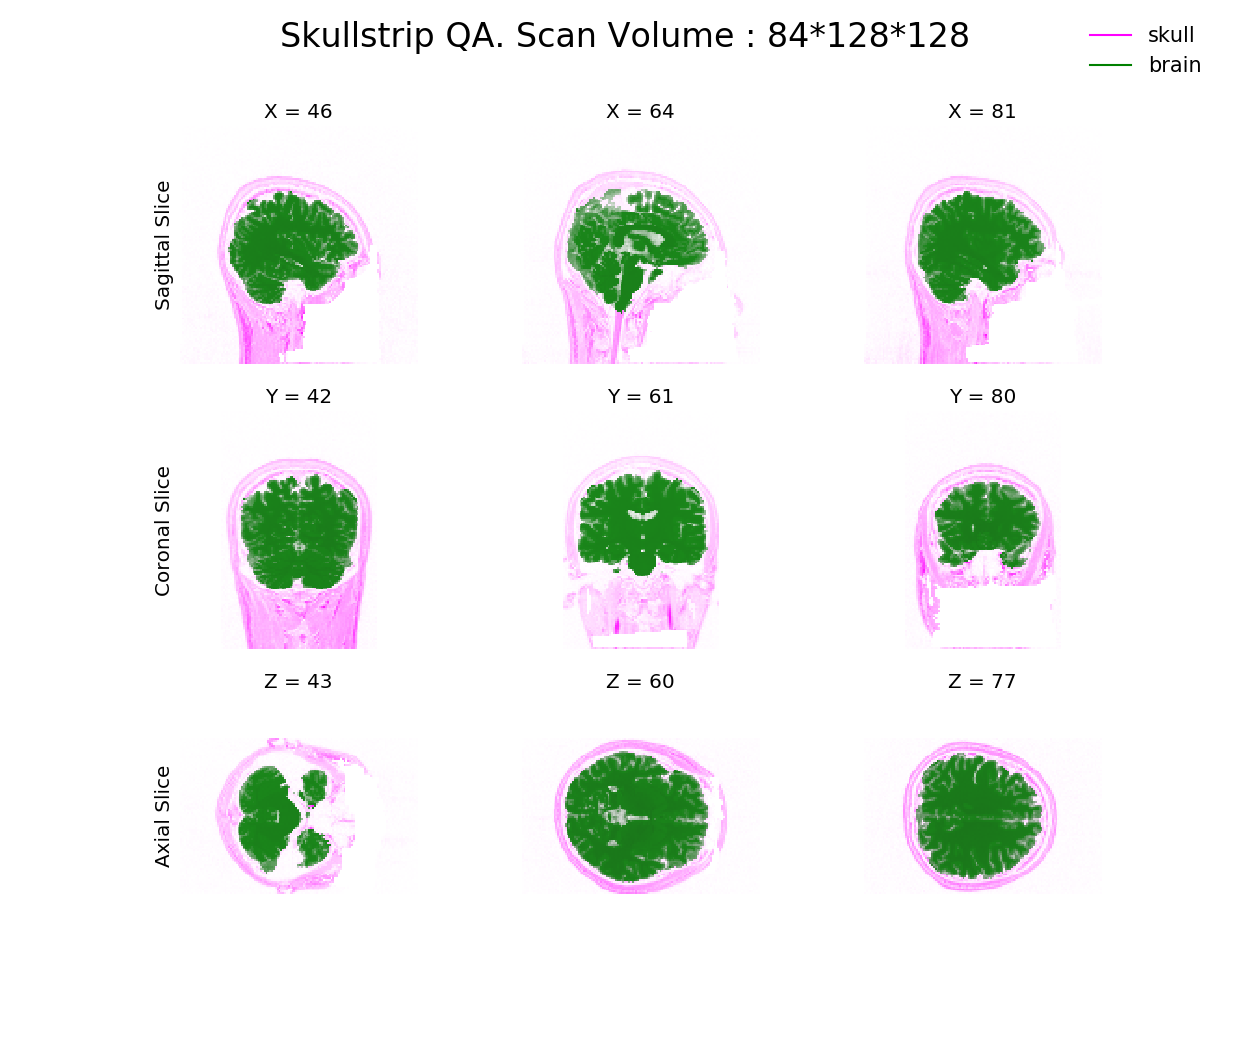
\includegraphics[width = 0.8\textwidth]{figures/m2g/diff_skullstip.png}
    \caption[Quality assurance figure from the \texttt{m2g-d} pipeline]{\textbf{Skull-stripping \texttt{m2g-d} QA} Quality assurance figure from the \texttt{m2g-d} pipeline displaying the skull-stripped brain (green) over the original anatomical image (magenta). Images are sampled from three locations along the sagittal, coronal, and axial reference directions.
    }
    \label{fig:diff_skull}
\end{figure}

\begin{figure}[h!]
    \centering
    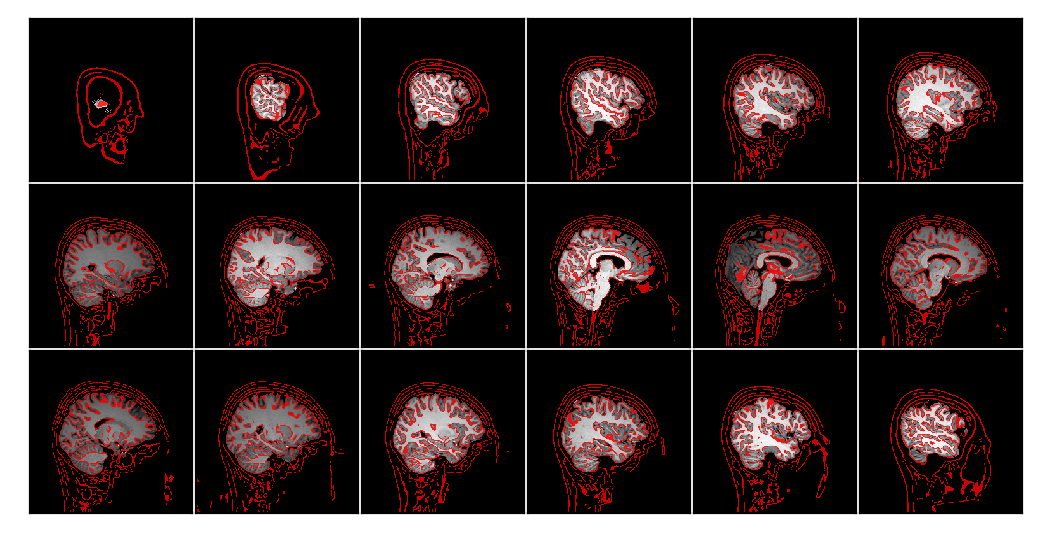
\includegraphics[width = 0.8\textwidth]{figures/m2g/func_skullstrip.png}
    \caption[Quality assurance figure from the \texttt{m2g-f} pipeline]{\textbf{Skull-stripping \texttt{m2g-f} QA} Quality assurance figure from the \texttt{m2g-f} pipeline displaying the skull stripped brain (white) and the outline of the removed skull (red). This particular output displays images from the sagittal reference direction, with another output displaying from the axial direction.
    }
    \label{fig:func_skull}
\end{figure}

\begin{figure}[h!]
    \centering
    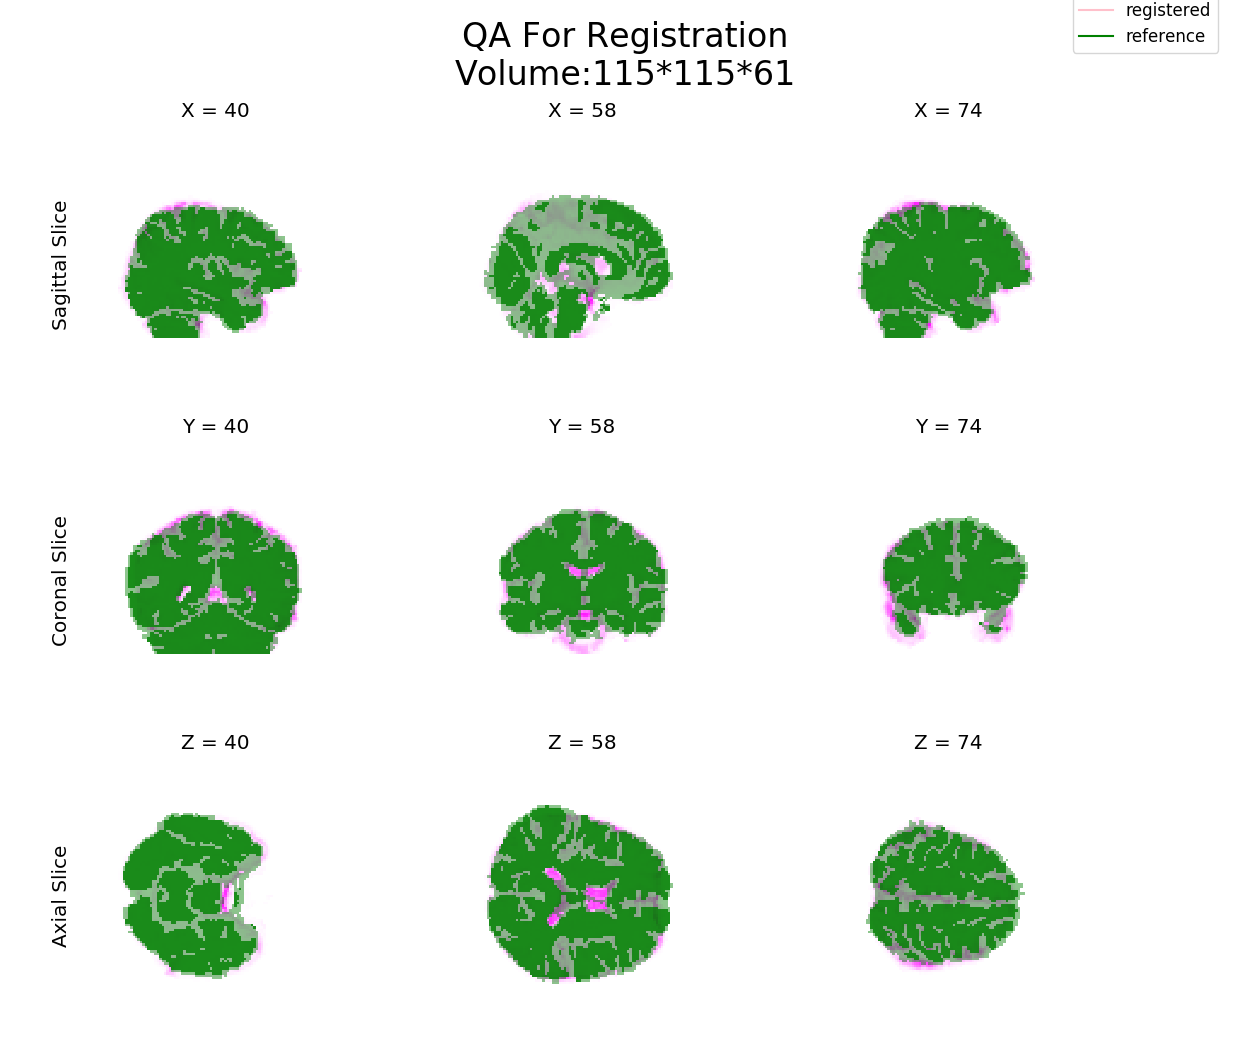
\includegraphics[width = 0.7\textwidth]{figures/m2g/diff_mapped_atlas.png}
    \caption[Quality assurance figure from the \texttt{m2g-d} pipeline displaying the registered Tissue parcellation (green) over the brain it is registered to from the anatomical image(magenta).]{\textbf{Parcellation Registration QA} Quality assurance figure from the \texttt{m2g-d} pipeline displaying the registered Tissue parcellation (green) over the brain it is registered to from the anatomical image(magenta). Images are sampled from three locations along the sagittal, coronal, and axial reference directions.
    }
    \label{fig:diff_mapped}
\end{figure}

\begin{figure}[h!]
    \centering
    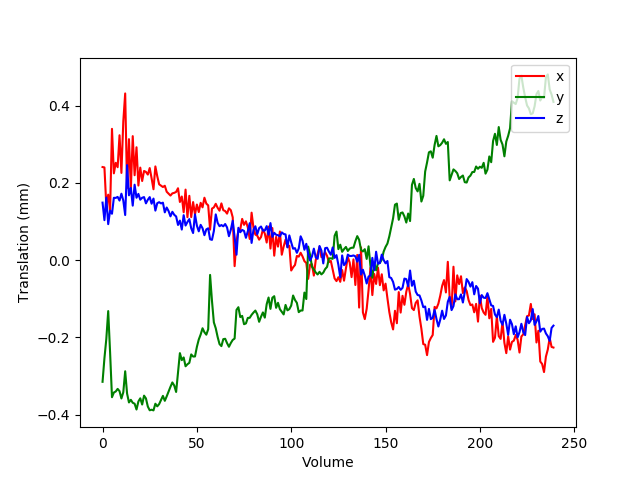
\includegraphics[width = 0.8\textwidth]{figures/m2g/func_motion_plot.png}
    \caption[ Quality assurance figure from the \texttt{m2g-f} pipeline which plots the distance in the x, y, and z axes that each functional volume was moved during the motion correction using AFNI's 3dvolreg.]{\textbf{Motion Correction QA} Quality assurance figure from the \texttt{m2g-f} pipeline which plots the distance in the x, y, and z axes that each functional volume was moved during the motion correction using AFNI's 3dvolreg.
    }
    \label{fig:func_motion}
\end{figure}
 % m2g
\chapter{graspologic} \label{chap:graspologic}

This chapter introduces our open-source Python package, designed to streamline network analysis for researchers like neuroscientists. It offers user-friendly implementations of the models and algorithms detailed in Chapters \ref{chap:statistical} and \ref{chap:nonpar}. This chapter was originally published in the Journal of Machine Learning Research in September 2019 (\url{http://jmlr.org/papers/v20/19-490.html}) and is distributed under the terms of a Creative Commons Attribution License that permits unrestricted use and redistribution provided that the original author and source are credited.

\begin{singlespace}         % you can also use onehalfspace to relax the spacing    
    \fullcite{chung2019graspy}.
\end{singlespace} 

\pagebreak

\section*{Abstract}
We introduce \graspy, a Python library devoted to statistical inference, machine learning, and visualization of random graphs and graph populations. This package  provides flexible and easy-to-use algorithms for analyzing and understanding graphs with a \sklearn compliant API. \graspy ~can be downloaded from Python Package Index (PyPi), and is released under the MIT open-source license. The documentation and all releases are available at \url{https://microsoft.github.io/graspologic/latest} and \url{https://github.com/microsoft/graspologic}, respectively.
\pagebreak


\section{Introduction}
Graphs, or networks, are a mathematical representation of data that consists of discrete objects (nodes or vertices) and relationships between these objects (edges). For example, if thinking of regions of a human brain as vertices, the edges can represent how strongly each pair of regions are connected to each other. 
Since graphs necessarily deal with relationships between nodes, many of the classical statistical assumptions about independence are violated. Thus, specific statistical methodology is required for performing robust statistical inference on graphs and populations of graphs \cite{survey-rdpg}. \graspy fills this gap by providing implementations of algorithms with strong statistical guarantees, such as graph and multi-graph embedding methods, two-graph hypothesis testing, and clustering of vertices of graphs. Many of the algorithms implemented in \graspy are flexible and can operate on graphs that are weighted or unweighted, as well as directed or undirected. All subsequent analysis in this thesis was performed using \graspy.

\section{Library Overview}
Overview of submodules available in \graspy is summarized in Figure \ref{fig:graspy}. The library contains functionality for fitting and sampling from random graph models, performing dimensionality reduction on graphs or populations of graphs (embedding), testing hypotheses on graphs, and plotting of graphs and embeddings.

The following provides brief overview of different submodules of \graspy, and more detailed overview and code usage can be found in the tutorial section of \graspy documentation at \url{https://microsoft.github.io/graspologic/latest/tutorials/index.html}.

\begin{figure}[t]
    \centering
    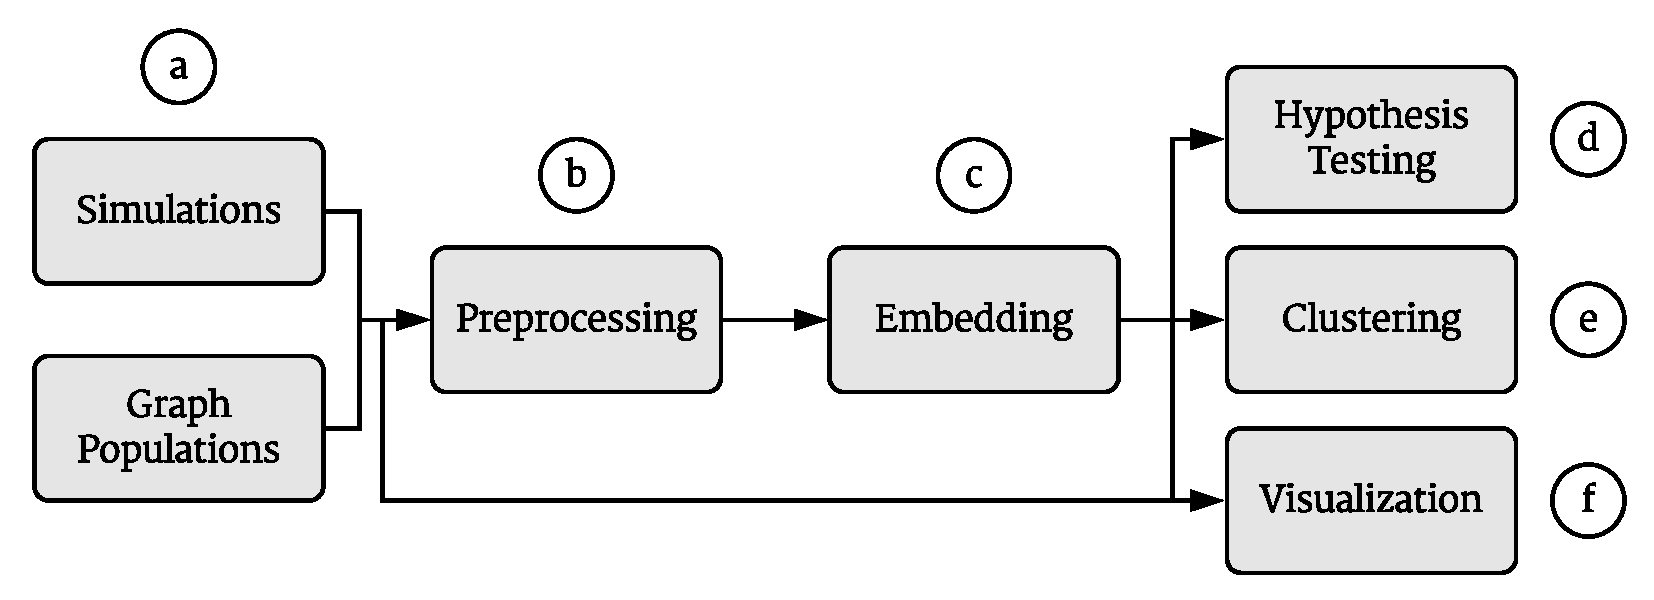
\includegraphics[width=.8\linewidth]{figures/graspy/graspy.pdf}
    \caption{Illustration of submodules and procedure for statistical inference on population of graphs. A detailed description of each submodule is given in section 2.}
    \label{fig:graspy}
\end{figure}

\subsection{Simulations (Figure \ref{fig:graspy}a)} Three classes of random graph models are implemented in \graspy: 1) Erd\H os-R\'enyi (ER) model, 2) stochastic block model (SBM), and 3) random dot product graph (RDPG) model. ER model is the simplest model, in which the model is parameterized by the number of vertices, $n$, and either $p$ that specifies a probability of an edge existing between a pair of vertices or $m$ that specifies the exact number of edges. All nodes have the same probability of connection to each other under the ER model. Unlike ER models, the SBM produces graphs containing communities, where vertices in each community share common probabilities of connection to every other community. The SBM is parameterized by the number of communities, $K$, a vector of probabilities of a node belonging to each community, $\tau$, and a probability matrix, $B\in[0,1]^{K \times K}$, that specifies the probability of edges within and between communities. An extension of the SBM, the Degree-corrected SBM (DCSBM) has an added parameter associated with each node that denotes its promiscuity in the graph, which is its relative degree among the other nodes in its community. Nodes still share the same relative probabilities of connection to each community, but the nodes within a community may have heterogeneous expected degrees. Finally, the RDPG model assumes that each vertex in the graph is associated with a latent vector in $\mathbb{R}^d$. The probability of an edge existing between pairs of vertices is determined by the dot product of the associated latent position vectors \cite{young2007random}. The RDPG is parameterized by an $n$ by $d$ matrix of these latent positions. \graspy provides implementations for sampling from each of these graph models given these parameters, as well as estimating the parameters of a model from a given graph. \graspy also allows for weighting functions and directed graphs when sampling from these models.

\subsection{Preprocessing (Figure \ref{fig:graspy}b)}
Various utility functions help the user input real data into \graspy or check simple attributes about a graph. Some examples include finding the largest connected component of a graph, finding the intersection or union of connected components across multiple graphs, transforming the weights of a graph, or checking whether a graph is directed. These functions speed the user's workflow when working with real data that may be messy or noisy before preprocessing.

\subsection{Embedding (Figure \ref{fig:graspy}c)}
Inference on random graphs depends on low-dimensional Euclidean representation of the vertices of graphs, known as \textit{latent positions}, typically given by spectral decompositions of adjacency or Laplacian matrices \cite{levin2017central}. Adjacency spectral embedding (ASE) and Laplacian spectral embedding (LSE) are methods for embedding a single graph, and omnibus embedding allows for embedding multiple graphs into the same dimensions such that the embeddings can be meaningfully compared. In addition, \graspy allows for the number of embedding dimensions to be automatically chosen by the algorithm of \cite{zhu2006automatic}. 

\begin{figure}[t!]
    \centering
    \includegraphics[width=1\textwidth]{figures/graspy/figure2.pdf}
    \caption
    [Connectome model fitting and complexity.  Larval Drosophila left mushroom body adjacency matrix (unweighted, directed), followed by random samples from four different statistical models of connectomes fit using \graspy]
    {Connectome model fitting and complexity.  Larval Drosophila left mushroom body adjacency matrix (unweighted, directed), followed by random samples from four different statistical models of connectomes fit using \graspy: random dot product graph (RDPG), degree-corrected stochastic block model (DCSBM), stochastic block model (SBM), and Erd\H os-R\'enyi (ER). The bottom left shows the number of parameters for each, as compared to the 40,000+ number of parameters (possible edges) for the inhomogeneous Erd\H os-R\'enyi (IER) model in which all potential edges are specified. Blocks are sorted by size (number of member vertices) and nodes are sorted by degree within each block. The block labels correspond to K) Kenyon cells, P) projection neurons, O) mushroom body output neurons, I) mushroom body input neurons \cite{eichler2017complete}.
    }
    \label{fig:my_label}
\end{figure}

\subsection{Hypothesis Testing (Figure \ref{fig:graspy}d)}
Given two graphs, a natural question to ask is whether these graphs are both random samples from the same generative distribution. \graspy provides two types of test for this null hypothesis: semiparametric and nonparametric. Both tests are framed under the RDPG model, where the generative distribution can be modeled as a set of latent positions. The semiparametric test can only be performed on two graphs of the same size and with known correspondence between the vertices of the two graphs \cite{tang2017semiparametric}. Nonparametric testing can be performed on graphs without vertex alignment, or even with different numbers of vertices \cite{tang2014nonparametric}. Both tests provide a statistically principled way of claiming whether two observed graphs are the same; for example, one can test whether the brain connectivity graphs of siblings or twins came from the same generative distribution (Chung et al., in preparation). 

\subsection{Clustering (Figure \ref{fig:graspy}e)}
\graspy uses Gaussian mixture models (GMM) and k-means to compute the grouping structure of vertices after embedding. The number of clusters to fit for GMM is chosen by Bayesian information criterion (BIC), which is a penalized likelihood function to evaluate the quality of estimators. Similarly, the silhouette score is used to choose the number of clusters for k-means. Both functions sweep over a range of parameters and use the above metrics to choose clustering parameters in an unsupervised manner. 

\subsection{Plotting (Figure \ref{fig:graspy}f)}
\graspy extends \texttt{seaborn} to visualize graphs as adjacency matrices and embedded graphs as paired scatter plots \cite{seaborn}. Individual graphs can be visualized using \texttt{heatmap} function, and multiple graphs can be overlaid on top of each other using \texttt{gridplot} function. Both adjacency matrix visualizations can be sorted by various node metadata. \texttt{pairplot} can visualize high dimensional data, such as graphs in the embedded space, as a pairwise scatter plot.

\section{Conclusion}
\graspy is the first open-source Python package to perform robust statistical analysis on graphs and graph populations. Its compliance with the \sklearn API makes it an easy-to-use tool for anyone familiar with machine learning in Python. In addition, \graspy is implemented with an extensible class structure, making it easy to modify and add new algorithms to the package. As \graspy continues to grow and add functionality, we believe it will accelerate statistically-valid discovery in any field of study concerned with populations of graphs.  %graspy
\chapter{Discussion}\label{chap:discussion}
\pagebreak

Models are important, but also should be used to understand the assumptions and can only make claims and limited to the assumptions of the models themselves. We hope that this thesis

This thesis presented novel methods for extracting principles from complex brain connectivity data, and demonstrated the application of these tools primarily on the connectome of a Drosophila larva brain. Despite these advances, many avenues remain for expanding upon this work and developing methods which will enable further biologically relevant inferences from connectome data.

\section{Value of Statistical Modeling}
\blindtext

\section{Where to go from here?}
\blindtext

%%%%%%%%%%%%%%%%%%%%%%%%%%%% END MAIN TEXT %%%%%%%%%%%%%%%%%%%%%%%%%%%%%





%%%%%%%%%%%%%%%%%%%%%%%%%%%%% BACK MATTER %%%%%%%%%%%%%%%%%%%%%%%%%%%%%%

%%%% BIBLIOGRAPHIC REFERENCES
\BibTextSpacing                     % one-half spacing for the bib items
\fancyhead[L]{\nouppercase \leftmark}

\chap{References}
\vspace{8pt}                % padding to compensate for single-spaced bibliography
\printbibliography[heading=none,notcategory=mypapers]             % include reference chapter


%%%% OPTIONAL: Appendix chapter (same format as the main chapters)
% \MainTextSpacing                    
% \fancyhead[L]{\appendixname\ \thechapter. \nouppercase \leftmark}

% %% necessary customization for the appendix and headers
\appendix 
\makeatletter
\addtocontents{toc}{\protect\renewcommand\protect\cftchappresnum{\@chapapp\ }}
\makeatother
\renewcommand{\thechapter}{\Alph{chapter}}

\chapter{Some necessary information}

% add your chapter text here
\Blindtext[3]
% \chapter{A few more additional information} \label{chap:appendix-b}

% add your chapter text here
\blindtext

%% add more appendix chapters as you need


%%%% biographical sketch or curriculum vitae
%% you can write it as a chapter and add it using \include{...} statement
% \include{14-biography}


%%%% if you already have a CV as a PDF, add it to the main directory:
% \includepdf[pages=-]{John_Doe_CV.pdf}

%%%%%%%%%%%%%%%%%%%%%%%%%%% END BACK MATTER %%%%%%%%%%%%%%%%%%%%%%%%%%%%

\end{document}

%%%%%%%%%%%%%%%%%%%%%%%%% DOCUMENT ENDS HERE %%%%%%%%%%%%%%%%%%%%%%%%%%%